% !TEX program = xelatex
\documentclass[UTF8,fontset=fandol,a4paper,11pt]{ctexart}
\usepackage[margin=21mm,top=23mm,bottom=22mm,headheight=16pt]{geometry}
\usepackage{amsmath,amssymb,mathtools,bm}
\usepackage{tikz}
\usetikzlibrary{arrows.meta,calc,angles,quotes,patterns}
\usepackage{xcolor,booktabs,array,longtable,enumitem,fancyhdr,needspace}
\usepackage[unicode,hidelinks]{hyperref}
\definecolor{ink}{HTML}{24343C}
\definecolor{accent}{HTML}{166A70}
\definecolor{muted}{HTML}{65747A}
\definecolor{rulegray}{HTML}{D4DDE0}
\definecolor{warm}{HTML}{966037}
\color{ink}
\setlength{\parindent}{2em}
\setlength{\parskip}{4pt}
\linespread{1.12}
\AtBeginDocument{\setlength{\abovedisplayskip}{6pt plus 2pt minus 1pt}
\setlength{\belowdisplayskip}{6pt plus 2pt minus 1pt}
\setlength{\abovedisplayshortskip}{0pt plus 1pt}
\setlength{\belowdisplayshortskip}{4pt plus 1pt}}
\setlist[enumerate]{label=(\arabic*),leftmargin=2.3em,itemsep=3pt,topsep=4pt}
\setlist[itemize]{leftmargin=2em,itemsep=2pt,topsep=4pt}
\allowdisplaybreaks[1]
\setlength{\emergencystretch}{2em}
\setcounter{secnumdepth}{0}
\providecommand{\tightlist}{\setlength{\itemsep}{0pt}\setlength{\parskip}{0pt}}
\ctexset{section={format=\Large\bfseries\color{accent},beforeskip=10pt,afterskip=9pt},
subsection={format=\normalsize\bfseries\color{accent},beforeskip=10pt,afterskip=4pt},
subsubsection={format=\normalsize\bfseries,beforeskip=8pt,afterskip=3pt}}
\pagestyle{fancy}
\fancyhf{}
\fancyhead[L]{\small\color{muted}物理学难题集萃}
% 页眉仅保留书名；版本名称只在封面显示。
\fancyfoot[L]{\small\color{muted}\chapterlabel}
\fancyfoot[R]{\small\thepage}
\renewcommand{\headrulewidth}{0.4pt}
\renewcommand{\footrulewidth}{0pt}
\newcommand{\dd}{\mathop{}\!\mathrm{d}}
\newcommand{\vect}[1]{\bm{#1}}
\newcommand{\tagline}[1]{\noindent{\small\color{muted}#1}\par}
\newcommand{\result}[1]{\begin{equation*}\boxed{#1}\end{equation*}}
\newcommand{\figcaption}[1]{\par\vspace{2pt}{\small\color{muted}#1}\par}
\newcommand{\teach}[2]{\Needspace{4\baselineskip}\subsection*{讲解要点与追问}#1\par\smallskip\noindent\textbf{追问：}#2\par}
\newcommand{\workarea}{\par\vspace{7mm}\noindent{\small\color{muted}作答区}\par\vspace{4mm}
\noindent\textcolor{rulegray}{\rule{\linewidth}{0.3pt}}\par\vspace{16mm}
\noindent\textcolor{rulegray}{\rule{\linewidth}{0.3pt}}\par\vspace{16mm}
\noindent\textcolor{rulegray}{\rule{\linewidth}{0.3pt}}\par\vspace{16mm}
\noindent\textcolor{rulegray}{\rule{\linewidth}{0.3pt}}}
\tikzset{axis/.style={-{Stealth[length=2mm]},thin,color=muted},
motion/.style={-{Stealth[length=2.3mm]},thick,color=accent},
force/.style={-{Stealth[length=2.3mm]},thick,color=warm},
traj/.style={thick,color=accent},guide/.style={dashed,thin,color=muted},
object/.style={thick,color=ink},every node/.style={font=\small}}\widowpenalty=10000\clubpenalty=10000\displaywidowpenalty=10000\newcommand{\chapterlabel}{电磁学第四章\quad 电流、直流电路}





\hypersetup{pdftitle={电磁学第四章 电流、直流电路·学生解答版},pdfauthor={}}

\begin{document}\pdfbookmark[0]{电磁学第四章 电流、直流电路}{cover}

\thispagestyle{empty}\vspace*{22mm}
\noindent{\Huge\bfseries 物理学难题集萃}\par\vspace{10mm}
\noindent{\LARGE 电磁学第四章}\par\vspace{6mm}
\noindent{\LARGE 电流、直流电路}\par\vspace{12mm}
\noindent{\Large\color{accent}学生解答版}\par\vspace{9mm}
\noindent\textcolor{accent}{\rule{\linewidth}{1pt}}\par\vspace{9mm}
\noindent 第1--35题\par\vfill\clearpage
\pdfbookmark[1]{题目目录}{contents}\section*{题目目录}
\begin{longtable}{@{}r p{113mm} r@{}}\toprule 题号 & 题目 & 页码\\\midrule

\hyperref[q:1]{1} & \hyperref[q:1]{导体表面充电与电荷弛豫} & \pageref{q:1} \\

\hyperref[q:2]{2} & \hyperref[q:2]{分段非均匀电导率中的体电荷和界面电荷} & \pageref{q:2} \\

\hyperref[q:3]{3} & \hyperref[q:3]{球对称大气导电与地面电势} & \pageref{q:3} \\

\hyperref[q:4]{4} & \hyperref[q:4]{双层漏电介质球的界面电荷} & \pageref{q:4} \\

\hyperref[q:5]{5} & \hyperref[q:5]{无碰撞双组分载流子的纵向小振动} & \pageref{q:5} \\

\hyperref[q:6]{6} & \hyperref[q:6]{增加两个相同电阻能否保持端口电阻} & \pageref{q:6} \\

\hyperref[q:7]{7} & \hyperref[q:7]{由三个端口测量反推六只电阻} & \pageref{q:7} \\

\hyperref[q:8]{8} & \hyperref[q:8]{三次测量识别八只电阻中的异值者} & \pageref{q:8} \\

\hyperref[q:9]{9} & \hyperref[q:9]{细分正四面体电阻网的两类端口} & \pageref{q:9} \\

\hyperref[q:10]{10} & \hyperref[q:10]{三个互相垂直圆环的等效电阻} & \pageref{q:10} \\

\hyperref[q:11]{11} & \hyperref[q:11]{无限梯形网络的收敛与有限阶通式} & \pageref{q:11} \\

\hyperref[q:12]{12} & \hyperref[q:12]{无限三角柱电阻网的对称折叠} & \pageref{q:12} \\

\hyperref[q:13]{13} & \hyperref[q:13]{七电阻单元串接成的无限网络} & \pageref{q:13} \\

\hyperref[q:14]{14} & \hyperref[q:14]{逐级折半的三角形导线网} & \pageref{q:14} \\

\hyperref[q:15]{15} & \hyperref[q:15]{三个方格的对角端口电阻} & \pageref{q:15} \\

\hyperref[q:16]{16} & \hyperref[q:16]{任意多个方格的对角端口电阻} & \pageref{q:16} \\

\hyperref[q:17]{17} & \hyperref[q:17]{四个方格网络的非对称端口} & \pageref{q:17} \\

\hyperref[q:18]{18} & \hyperref[q:18]{双圆环等分电阻网的相邻异层端口} & \pageref{q:18} \\

\hyperref[q:19]{19} & \hyperref[q:19]{无限点阵任意两节点间的电阻} & \pageref{q:19} \\

\hyperref[q:20]{20} & \hyperref[q:20]{星形与三角形的端口等效及应用} & \pageref{q:20} \\

\hyperref[q:21]{21} & \hyperref[q:21]{四乘四方格网的对角电阻} & \pageref{q:21} \\

\hyperref[q:22]{22} & \hyperref[q:22]{立方体表面细分网络的相邻面心端口} & \pageref{q:22} \\

\hyperref[q:23]{23} & \hyperref[q:23]{灯泡分压供电的效率与变阻器额定值} & \pageref{q:23} \\

\hyperref[q:24]{24} & \hyperref[q:24]{随机断路电桥的平均功率} & \pageref{q:24} \\

\hyperref[q:25]{25} & \hyperref[q:25]{并联电源组的等效电动势与内阻} & \pageref{q:25} \\

\hyperref[q:26]{26} & \hyperref[q:26]{惠斯通电桥的平衡与微小失衡电流} & \pageref{q:26} \\

\hyperref[q:27]{27} & \hyperref[q:27]{含对角支路的广义电桥平衡} & \pageref{q:27} \\

\hyperref[q:28]{28} & \hyperref[q:28]{保留精密分流器修复三量程电流表} & \pageref{q:28} \\

\hyperref[q:29]{29} & \hyperref[q:29]{二值输入电阻梯的最大输出电压} & \pageref{q:29} \\

\hyperref[q:30]{30} & \hyperref[q:30]{十电容对称网络的等效电容} & \pageref{q:30} \\

\hyperref[q:31]{31} & \hyperref[q:31]{电容星三角变换及九电容网络} & \pageref{q:31} \\

\hyperref[q:32]{32} & \hyperref[q:32]{一步与逐级充电的能量损耗} & \pageref{q:32} \\

\hyperref[q:33]{33} & \hyperref[q:33]{三只预充电容的部分放电} & \pageref{q:33} \\

\hyperref[q:34]{34} & \hyperref[q:34]{匹配电容梯的能量及截断后的重分布} & \pageref{q:34} \\

\hyperref[q:35]{35} & \hyperref[q:35]{含电源与电容的立方体稳态网络} & \pageref{q:35} \\

\bottomrule\end{longtable}

本章采用SI单位。电压$U_{AB}=V_A-V_B$，电流按图示箭头取正，计算为负表示实际方向相反。电容网络除特别给出预充电荷外，内部浮置导体的初始净电荷为零。无限网络采用无背景驱动的有限无源网络极限；投影交叉只在标明节点处电连接。

\clearpage

\pdfbookmark[2]{第 1 题 导体表面充电与电荷弛豫}{q1}

\section*{第 1 题\quad 导体表面充电与电荷弛豫}\label{q:1}

一长方体导体起初不带净电荷。$t=0$时开始施加垂直于两相对大表面的恒定均匀电场$\vect E_0$。导体电导率$\sigma$为常量，自由电子到达两端后停留在表面，忽略边缘效应。用这一欧姆导电的简化模型，求两端积累的面电荷密度和内部电流密度随时间的变化。

\begin{center}\begin{minipage}{.98\linewidth}\centering
\begin{tikzpicture}[scale=.9,transform shape]

\fill[accent!8](0,0) rectangle(3,2.6);\draw[object](0,0) rectangle(3,2.6);
\node[above] at(0,2.6){$-s(t)$};\node[above] at(3,2.6){$+s(t)$};
\draw[motion](-1.4,1.7)--(-.3,1.7) node[midway,above]{$E_0$};\draw[motion](3.3,1.7)--(4.4,1.7) node[midway,above]{$E_0$};
\draw[force](.7,1.3)--(2.3,1.3) node[midway,above]{$j(t)$};
\draw[axis](-.4,-.5)--(4,-.5) node[right]{$x$};\node at(6,1.3){电导率$\sigma$恒定};

\end{tikzpicture}
\figcaption{图电4.1\quad 外加场向右，左右表面积累等量异号电荷。}
\end{minipage}\end{center}

\Needspace{6\baselineskip}\subsection*{解答}

取图电4.1中向右为正。左表面带负电，右表面带正电；用$s(t)\ge0$表示面密度的大小，两面的实际值分别为$-s,+s$。解图电4.1A把外加场与积累电荷的反向场分开。

\begin{center}\begin{minipage}{.98\linewidth}\centering
\begin{tikzpicture}[scale=.9,transform shape]

\draw[motion](0,1.8)--(3,1.8) node[midway,above]{$\vect E_0$};
\draw[force](2.4,.8)--(.6,.8) node[midway,above]{$\vect E'=-s\vect e_x/\varepsilon_0$};
\draw[axis](5,0)--(10,0) node[right]{$t/\tau$};\draw[axis](5,0)--(5,2.7) node[above]{归一化量};
\draw[traj,domain=0:4.4,samples=50] plot({5+\x},{2.1*(1-exp(-\x))});
\draw[force,domain=0:4.4,samples=50] plot({5+\x},{2.1*exp(-\x)});
\draw[guide](5,2.1)--(9.6,2.1);\node[left] at(5,2.1){$1$};
\node at(8,1.55){$s/(\varepsilon_0E_0)$};\node at(7,.25){$j/(\sigma E_0)$};

\end{tikzpicture}
\figcaption{解图电4.1A\quad 反场随面电荷建立；两条归一化曲线之和恒为1。}
\end{minipage}\end{center}

两个很大的异号面产生的内部场大小为$s/\varepsilon_0$，所以总场、电流密度及表面电荷增长率为
\[
E=E_0-\frac{s}{\varepsilon_0},\qquad j=\sigma E,\qquad \frac{\dd s}{\dd t}=j.
\]
最后一式来自右端面积$A$上的电荷守恒：$A\dd s=(jA)\dd t$，流入薄层的电荷增量与储存在端面的电荷增量均与面积 $A$ 成正比，故两侧约去同一个 $A$。于是
\[
\frac{\dd s}{\dd t}+\frac{\sigma}{\varepsilon_0}s=\sigma E_0,
\qquad s(0)=0.
\]
令$\tau=\varepsilon_0/\sigma$。分离变量或乘积分因子$e^{t/\tau}$，得到
\[
\int_0^s\frac{\dd u}{\varepsilon_0E_0-u}=\frac t\tau,
\qquad
\boxed{s(t)=\varepsilon_0E_0(1-e^{-t/\tau})}.
\]
代回总场和欧姆定律：
\[
\boxed{E(t)=E_0e^{-t/\tau},\qquad j(t)=\sigma E_0e^{-t/\tau}}.
\]
解图电4.1A中上升的$s/(\varepsilon_0E_0)$与下降的$j/(\sigma E_0)$之和恒为1，反映积累电荷逐步屏蔽外场。初始$s=0,j=\sigma E_0$；足够晚后$s\to\varepsilon_0E_0,j\to0$，导体内达到静电平衡。

若两表面间距为 $d$，单位表面积对应的导体体积是 $d$，将单位体积的焦耳功率对时间积分：
\[
\frac{Q_J}{A}=\int_0^\infty\sigma E^2d\dd t
=\frac12\varepsilon_0E_0^2d.
\]
外加场由装置维持。上式计算的是导体内部的焦耳耗散。欧姆模型把电流视为随局部场即时改变，采用准静态平面场，对应时间常数 $\tau$。

\begin{center}\begin{minipage}{.97\linewidth}\centering
\begin{tikzpicture}[x=1cm,y=1cm,font=\small]
\fill[accent!8](0,0)rectangle(3,2);\draw[object](0,0)rectangle(3,2);
\draw[guide](2.5,-.25)rectangle(3.5,2.25);\node[above]at(3,2.3){右端薄层};
\draw[motion](1.2,1.3)--(2.8,1.3)node[midway,above]{$jA$};
\draw[force](1.8,.65)--(.5,.65)node[midway,below]{电子漂移};
\node[right]at(3.7,1.6){$Q=sA$};\node[right]at(3.7,.8){$\dot Q=jA$};
\node[right]at(3.7,0){外侧没有传导电流};
\end{tikzpicture}
\figcaption{解图电4.1B　右端控制薄层。正向传导电流流入薄层，电子向左移动使右面留下正电荷。}
\end{minipage}\end{center}
\begin{center}\begin{minipage}{.97\linewidth}\centering
\begin{tikzpicture}[x=4.1cm,y=2.7cm,font=\small]
\draw[axis](0,0)--(1.22,0)node[below right]{$s/s_\infty$};
\draw[axis](0,0)--(0,1.25)node[above]{$j/j_0$};
\draw[traj](0,1)--(1,0);\node[left]at(0,1){$1$};\node[below]at(1,0){$1$};
\fill(0,1)circle(1.4pt);\fill(.63212,.36788)circle(1.4pt);\fill(.86466,.13534)circle(1.4pt);
\node[above right]at(0,1){$t=0$};\node[above right]at(.63212,.36788){$t=\tau$};
\node[above right]at(.86466,.13534){$t=2\tau$};
\draw[guide](.63212,0)--(.63212,.36788)--(0,.36788);
\node[right,align=left]at(1.35,.72){$s_\infty=\varepsilon_0E_0$\\$j_0=\sigma E_0$\\$j/j_0+s/s_\infty=1$};
\end{tikzpicture}
\figcaption{解图电4.1C　电流与积累面电荷的实际对应关系。过程沿线段由左上向右下推进，时间等间隔的点并不等距。}
\end{minipage}\end{center}

解图电4.1B把电荷守恒落实到右端薄层。薄层左侧有$jA$流入，右侧没有传导电流流出，因而$\dot Q=jA$。
左端薄层则有正向电流流出，所以其带符号面密度满足$\dd(-s)/\dd t=-j$；两式相加给两端总电荷始终为零。
导体内部$j$在空间上均匀，$\partial j/\partial x=0$，故这一模型没有额外体电荷积累。各相邻薄层间没有电流差，积累发生在传导电流终止的两端。

解图电4.1C将两个时间函数消去t，得到$j/j_0=1-s/s_\infty$。
图上每一点的 $j$ 给对应时刻 $s$ 曲线的切线斜率。例如$t=\tau$时，面电荷达到最终值的$0.6321$，电流仍为初值的$0.3679$。
面积 $A$ 将面密度换成总电荷 $Q=sA$。厚度 $d$ 将场强换成内电压 $Ed$，并进入耗散能量。弛豫时间的长度独立性来自均匀电导率和平面场。

恒定外场阶段，传导电流和位移电流沿同一轴计算。$t>0$且外加场恒定时，$\varepsilon_0\dot E=-\dot s=-j$，所以传导电流与位移电流之和为零。
导体内部的载流子仍在向端面输运，同一位置的位移电流与传导电流反向。外场刚接通的理想阶跃涉及开关瞬间的位移响应，本题的指数过程从接通后的初值开始计算。
对真实材料，只有在欧姆关系能跟随场的变化、并可采用准静态平面场时，这个一阶模型才适用。


\Needspace{23\baselineskip}

\pdfbookmark[2]{第 2 题 分段非均匀电导率中的体电荷和界面电荷}{q2}

\section*{第 2 题\quad 分段非均匀电导率中的体电荷和界面电荷}\label{q:2}

截面积为$S$、长$2L$的圆柱导体沿轴向坐标$x$的电导率为
\[
\sigma(x)=\begin{cases}\sigma_0(1+x/L),&0<x<L,\\\sigma_0(1+2x/L),&L<x<2L.\end{cases}
\]
两端电压$\Delta U=U(0)-U(2L)>0$，稳恒电流沿$+x$均匀通过每个截面。介电响应取真空值$\varepsilon_0$，忽略边缘效应。求总电阻、$x\ne L$处体电荷密度，以及$x=L$处自由面电荷密度。

\begin{center}\begin{minipage}{.98\linewidth}\centering
\begin{tikzpicture}[scale=.9,transform shape]

\fill[accent!8](0,0) rectangle(3,1.8);\fill[warm!10](3,0) rectangle(6,1.8);\draw[object](0,0) rectangle(6,1.8);
\draw[guide](3,-.2)--(3,2);\node at(1.5,1.25){$\sigma_0(1+x/L)$};\node at(4.5,1.25){$\sigma_0(1+2x/L)$};
\draw[motion](.7,.55)--(2.2,.55) node[midway,above]{$I$};\node[above] at(0,1.8){$U(0)$};\node[above] at(6,1.8){$U(2L)$};
\draw[axis](-.4,-.55)--(6.5,-.55) node[right]{$x$};\foreach \x/\s in {0/0,3/L,6/{2L}}{\node[below] at(\x,-.55){$\s$};}
\node[right] at(6,1){截面$S$};

\end{tikzpicture}
\figcaption{图电4.2\quad 两段串联，电流通过同一截面积，电导率在中间界面跳变。}
\end{minipage}\end{center}

\Needspace{6\baselineskip}\subsection*{解答}

图电4.2的电导率在$x=L$由$2\sigma_0$跃变到$3\sigma_0$。各截面通过同一个稳恒电流，截面积也相同，故电流密度 $j$ 为常量。场强随局部电导率变化。定义
\[
k=\ln2+\frac12\ln\frac53=0.94855999\ldots .
\]
把长度$\dd x$的小片看成串联微元，完整积分为
\[
R=\frac1S\int_0^{2L}\frac{\dd x}{\sigma(x)}
=\frac{L}{\sigma_0S}\left(\int_0^1\frac{\dd u}{1+u}+\int_1^2\frac{\dd u}{1+2u}\right)
=\boxed{\frac{kL}{\sigma_0S}}.
\]
因此$I=\sigma_0S\Delta U/(kL)$，$j=\sigma_0\Delta U/(kL)$。解图电4.2A以同一$j$贯穿两段，并画出场强的下降及界面跃变。

\begin{center}\begin{minipage}{.98\linewidth}\centering
\begin{tikzpicture}[scale=.9,transform shape]

\draw[axis](0,0)--(5,0) node[right]{$x/L$};\draw[axis](0,0)--(0,3) node[above]{$E\sigma_0/j$};
\draw[traj,domain=0:1,samples=35] plot({2*\x},{2.5/(1+\x)});
\draw[traj,domain=1:2,samples=35] plot({2*\x},{2.5/(1+2*\x)});
\draw[guide](2,0)--(2,1.5);\fill(2,1.25) circle(1.5pt);\fill(2,.8333) circle(1.5pt);
\node[above right] at(2,1.25){$1/2$};\node[below left] at(2,.8333){$1/3$};\node[below] at(2,0){$1$};\node[below] at(4,0){$2$};
\draw[object](6,0) rectangle(9,2);\draw[guide](7.5,-.2)--(7.5,2.2);\node[above] at(7.5,2.2){$x=L,\ s_L<0$};
\draw[axis](6,1)--(5.5,1);\draw[axis](9,1)--(9.5,1);\node[below] at(6,0){$L^-$};\node[below] at(9,0){$L^+$};
\node[align=center] at(7.5,-.75){高斯面通量\\$[E(L^+)-E(L^-)]S$};

\end{tikzpicture}
\figcaption{解图电4.2A\quad 左图的场强下跳对应负界面电荷；右图明确高斯面两侧的外法线。}
\end{minipage}\end{center}

欧姆定律和一维高斯定律给
\[
E(x)=\frac{j}{\sigma(x)},\qquad \rho_e=\varepsilon_0\frac{\dd E}{\dd x}.
\]
在两段内部逐项求导：
\[
\boxed{\rho_e(x)=\begin{cases}
-\dfrac{\varepsilon_0\Delta U}{kL^2(1+x/L)^2},&0<x<L,\\[3pt]
-\dfrac{2\varepsilon_0\Delta U}{kL^2(1+2x/L)^2},&L<x<2L.
\end{cases}}
\]
电导率递增而$j$不变，场强沿$x$减小，体电荷因而为负。界面两侧场强为
\[
E(L^-)=\frac{j}{2\sigma_0},\qquad E(L^+)=\frac{j}{3\sigma_0}.
\]
取薄柱高斯面，右端外法线沿$+x$、左端沿$-x$，有$[E(L^+)-E(L^-)]S=s_LS/\varepsilon_0$，故
\[
\boxed{s_L=-\frac{\varepsilon_0j}{6\sigma_0}=-\frac{\varepsilon_0\Delta U}{6kL}}.
\]
界面带负电，面密度大小约为 $0.1757\varepsilon_0\Delta U/L$。体密度描述各开区间内场强的连续变化，面密度对应界面处的一次有限跃变。

将两段体电荷与中间界面电荷按单位截面积相加，得到：
\[
\int_{0^+}^{L^-}\rho_e\dd x+s_L+\int_{L^+}^{2L^-}\rho_e\dd x
=\varepsilon_0[E(2L^-)-E(0^+)]
=-\frac{4\varepsilon_0j}{5\sigma_0}.
\]
这里的积分区间从左端内侧延伸到右端内侧。导体两端与外接装置交界处的面电荷由各端面两侧的电场决定。

\begin{center}\begin{minipage}{.97\linewidth}\centering
\begin{tikzpicture}[x=2.65cm,y=2.7cm,font=\small]
\draw[axis](0,0)--(2.3,0)node[below right]{$u=x/L$};
\draw[axis](0,0)--(0,1.25)node[above]{$[U(x)-U(2L)]/\Delta U$};
\draw[traj,domain=0:1,samples=65,variable=\t]plot(\t,{1-ln(1+\t)/.9485599924});
\draw[traj,domain=1:2,samples=65,variable=\t]plot(\t,{1-(ln(2)+.5*ln((1+2*\t)/3))/.9485599924});
\draw[guide](1,0)--(1,.26927)--(0,.26927);
\fill(1,.26927)circle(1.4pt);\node[above right]at(1,.26927){连续，斜率改变};
\node[left]at(0,1){$1$};\node[below]at(1,0){$1$};\node[below]at(2,0){$2$};
\end{tikzpicture}
\figcaption{解图电4.2B　由场强分段积分得到的电势。界面没有有限电势跃变，电势曲线在此连续而不光滑。}
\end{minipage}\end{center}

解图电4.2B画出由$U'=-E$积分得到的电势。在中间界面，两段曲线的电势相接，斜率分别取两侧电场的相反数。令$u=x/L$，在两段分别积分可得
\[
\frac{U(x)-U(2L)}{\Delta U}=\begin{cases}
1-\dfrac{\ln(1+u)}k,&0\le u\le1,\\[3pt]
1-\dfrac{\ln2+\tfrac12\ln[(1+2u)/3]}k,&1\le u\le2.
\end{cases}
\]
两式在$u=1$给同一个$1-\ln2/k$，但左右斜率之比为$3/2$，与A图的场强比相同。
电场虽有有限跃变，跨越趋于零厚度的界面时，其电势积分趋于零。
\begin{center}\begin{minipage}{.97\linewidth}\centering
\begin{tikzpicture}[x=2.65cm,y=3cm,font=\small]
\draw[axis](0,0)--(2.35,0)node[right]{$u=x/L$};
\draw[axis](0,-.95)--(0,.27)node[above]{$q(x)/(\varepsilon_0j/\sigma_0)$};
\draw[traj,domain=0:1,samples=60,variable=\t]plot(\t,{1/(1+\t)-1});
\draw[traj,domain=1:2,samples=60,variable=\t]plot(\t,{1/(1+2*\t)-1});
\draw[force](1,-.5)--(1,-.666667);\draw[guide](0,-.8)--(2,-.8);
\node[left]at(0,-.8){$-4/5$};\node[above left]at(1,-.5){$-1/2$};
\draw[guide](1,-.666667)--(1.25,-.56);\node[right]at(1.25,-.56){$-2/3$};
\node[above]at(1,0){$1$};\node[above]at(2,0){$2$};
\node[right,align=left]at(2.45,-.4){界面增量\\$\Delta q=s_L$};
\end{tikzpicture}
\figcaption{解图电4.2C　从左端内部起累计的单位截面积电荷。曲线在界面向下跳$\varepsilon_0j/(6\sigma_0)$，两端外表面电荷不在此图范围内。}
\end{minipage}\end{center}

解图电4.2C把体电荷积分和界面面电荷放在同一条累计曲线上。
定义$q(x)$为$0^+$到x之间的电荷除以截面积S，若x跨过L就计入$s_L$，由高斯定律有$q(x)=\varepsilon_0[E(x)-E(0^+)]$。
第一段终点$q(L^-)=-\varepsilon_0j/(2\sigma_0)$；跨界面后$q(L^+)=-2\varepsilon_0j/(3\sigma_0)$；第二段再贡献$-2\varepsilon_0j/(15\sigma_0)$，终点为$-4\varepsilon_0j/(5\sigma_0)$。
累计曲线先因两段内各自的负体电荷下降，再将界面的面电荷作为一个单独的下跳计入。

负体电荷和负界面电荷是维持稳恒场分布的静态电荷。任意小段有相同的$jS$流入和流出，因此净积累率为零；局部留下的电荷维持所求的静态场强分布。
界面电荷由场强的跳变量决定。两侧场都沿正x方向，且右侧场强小于左侧，所以从左向右跨界面时场强跳变量为负，面电荷也为负。


\Needspace{13\baselineskip}

\pdfbookmark[2]{第 3 题 球对称大气导电与地面电势}{q3}

\section*{第 3 题\quad 球对称大气导电与地面电势}\label{q:3}

把地球视为半径$R=6.0\times10^6\,\mathrm m$的导体。晴天大气的球对称电导率为$\sigma(r)=\sigma_0+a(r-R)^2$，其中$\sigma_0=3.0\times10^{-14}\,\mathrm{S/m}$，$a=0.5\times10^{-20}\,\mathrm{S/m^3}$。径向向外为正，已知$E(R)=-100\,\mathrm{V/m}$。采用稳态近似，大气电荷分布不变，忽略地球内部体电荷。求流入地面的总电流大小、地面自由面电荷密度、大气体电荷分布，以及大气顶层$r\to\infty$相对地面的电势差。

\begin{center}\begin{minipage}{.98\linewidth}\centering
\begin{tikzpicture}[scale=.9,transform shape]

\fill[accent!8](0,0) circle(1.8);\draw[object](0,0) circle(1.8);\draw[guide](0,0) circle(2.7);
\node at(0,0){地球};\draw[axis](0,0)--(1.273,1.273) node[midway,above left]{$R$};
\foreach \a in {0,90,180,270}{\draw[force](\a:2.5)--(\a:1.95);}
\node[right] at(2.8,1.3){$\rho_e(r)>0$};\node[right] at(2.8,.4){$E_R<0$};\node[right] at(2.8,-.5){$s_R<0$};

\end{tikzpicture}
\figcaption{图电4.3\quad 径向向外为正，地面带负电，大气电场及传导电流向内。}
\end{minipage}\end{center}

\Needspace{6\baselineskip}\subsection*{解答}

图电4.3中的电流沿径向向内，同心球面越大，单位面积通过的电流越小。先在地面使用欧姆定律：
\[
j(R)=\sigma_0E_R,\qquad
\boxed{I=4\pi R^2\sigma_0|E_R|\simeq1.36\times10^3\,\mathrm A},
\quad E_R=E(R).
\]
导体内场为零，跨过地面的小高斯柱给
\[
\boxed{s_R=\varepsilon_0E_R=-8.85\times10^{-10}\,\mathrm{C/m^2}}.
\]

\begin{center}\begin{minipage}{.98\linewidth}\centering
\begin{tikzpicture}[scale=.9,transform shape]

\draw[object](0,0) circle(1);\draw[guide](0,0) circle(2);\draw[guide](0,0) circle(2.3);
\draw[axis](0,0)--(2,0) node[midway,below]{$r$};\draw[<->](2,.4)--(2.3,.4);\node[right] at(2.3,.4){$\dd r$};
\draw[force](0,2.7)--(0,1.7) node[left]{$j$};\node at(0,-2.8){$4\pi r^2j(r)=-I$};
\node[align=left] at(6,1){球壳体积$4\pi r^2\dd r$\\外减内的通量\\$4\pi\dd(r^2E)$};
\node[align=left] at(6,-1.2){$\Delta V=-\int_R^\infty E\dd r>0$\\顶层电势高于地面};

\end{tikzpicture}
\figcaption{解图电4.3A\quad 同心球面上的总电流相同；球壳电荷由两面的电通量之差求出。}
\end{minipage}\end{center}

解图电4.3A取半径$r,r+\dd r$的球壳。稳恒电流要求$4\pi r^2j(r)=4\pi R^2j(R)$，所以
\[
j(r)=\sigma_0E_R\frac{R^2}{r^2},\qquad
\boxed{E(r)=\frac{\sigma_0E_RR^2}{r^2[\sigma_0+a(r-R)^2]}}.
\]
用球壳内电荷等于两球面电通量之差，有
\[
\rho_e=\frac{\varepsilon_0}{r^2}\frac{\dd(r^2E)}{\dd r}
=\boxed{-\frac{2\varepsilon_0\sigma_0E_RR^2a(r-R)}{r^2[\sigma_0+a(r-R)^2]^2}}.
\]
由于$E_R<0$，$r>R$的体电荷为正，符合图示。球面的面积随半径增大，展开通量导数得到 $\varepsilon_0(E'+2E/r)$。

电势差按所问的顶层减地面定义：
\[
\Delta V=V(\infty)-V(R)=-\int_R^\infty E(r)\dd r>0.
\]
令$h=\sqrt{\sigma_0/a}$、$z=r-R$，则
\[
\Delta V=-E_RR^2h^2\int_0^\infty\frac{\dd z}{(R+z)^2(z^2+h^2)}.
\]
对被积函数作分式分解，记$D=R^2+h^2$：
\[
\frac1{(R+z)^2(z^2+h^2)}
=\frac{2R}{D^2(R+z)}+\frac1{D(R+z)^2}
-\frac{2Rz}{D^2(z^2+h^2)}+\frac{R^2-h^2}{D^2(z^2+h^2)}.
\]
积分时两个对数的无穷部分相消，结果为
\[
\boxed{\Delta V=-E_R\frac{R^2h^2}{D^2}
\left[\frac D R+2R\ln\frac hR+\frac{\pi(R^2-h^2)}{2h}\right]
\simeq3.83\times10^5\,\mathrm V}.
\]
本题$h\simeq2.45\times10^3\,\mathrm m\ll R$。若在近地主要导电层用$r^2\simeq R^2$，可估为$\Delta V\simeq|E_R|\pi h/2=3.85\times10^5\,\mathrm V$。主要电压降出现在几倍 $h$ 以内，因而用平面面积给出相差约 $0.38\%$ 的近地估算。

再积分体电荷，可得$Q_{\rm atm}=4\pi\varepsilon_0[r^2E]_R^\infty=-4\pi\varepsilon_0R^2E_R$，与地面总负电荷相抵消。这里取地面场强为给定条件，该场强在模型中维持稳态径向电流。

\begin{center}\begin{minipage}{.97\linewidth}\centering
\begin{tikzpicture}[x=1.45cm,y=2.7cm,font=\small]
\draw[axis](0,0)--(4.4,0)node[below right]{$u=(r-R)/h$};
\draw[axis](0,0)--(0,1.25)node[above]{归一化密度与场强};
\draw[traj,domain=0:4,samples=100,variable=\t]plot(\t,{1/((1+\t*\t)*(1+.0004082483*\t)^2)});
\draw[thick,warm,domain=0:4,samples=100,variable=\t]plot(\t,{2*\t/((1+\t*\t)^2*(1+.0004082483*\t)^2)});
\node[left]at(0,1){$1$};\node[below]at(1,0){$1$};\node[below]at(2,0){$2$};
\node[right,accent]at(4.7,.95){$E/E_R$};
\node[right,warm]at(4.7,.5){$\rho_e/(\varepsilon_0|E_R|/h)$};
\end{tikzpicture}
\figcaption{解图电4.3B　按给定球对称模型绘制的场强比与正体电荷密度。两条曲线保留$r^{-2}$因子；场向内，正电荷密度在近地处先升后降。}
\end{minipage}\end{center}

解图电4.3B用$u=(r-R)/h$、$\eta=h/R$将两个空间分布写为
\[
\frac{E}{E_R}=\frac1{(1+u^2)(1+\eta u)^2},\qquad
\frac{\rho_e}{\varepsilon_0|E_R|/h}=\frac{2u}{(1+u^2)^2(1+\eta u)^2}.
\]
图中的 $E/E_R$ 为正，对应向内的负径向场。体密度在地面为零，向上先增大再减小。两条曲线均保留球面面积随高度增长的因子 $(1+\eta u)^{-2}$。
\begin{center}\begin{minipage}{.97\linewidth}\centering
\begin{tikzpicture}[x=1.45cm,y=2.7cm,font=\small]
\draw[axis](0,0)--(4.4,0)node[below right]{$u=(r-R)/h$};
\draw[axis](0,0)--(0,1.25)node[above]{电荷比例};
\draw[traj,domain=0:4,samples=100,variable=\t]plot(\t,{1/(1+\t*\t)});
\draw[thick,warm,domain=0:4,samples=100,variable=\t]plot(\t,{\t*\t/(1+\t*\t)});
\draw[guide](1,0)--(1,.5)--(0,.5);\fill(1,.5)circle(1.4pt);
\node[left]at(0,1){$1$};\node[left]at(0,.5){$1/2$};\node[below]at(1,0){$1$};
\node[right,accent]at(4.7,.85){$Q_{\rm enc}/Q_{\rm g}$};
\node[right,warm]at(4.7,.4){$Q_{\rm atm}(<r)/|Q_{\rm g}|$};
\end{tikzpicture}
\figcaption{解图电4.3C　有限球面内的总负电荷比例与累计大气正电荷比例。两者在高度h处均为1/2，只有到无穷远才完全抵消。}
\end{minipage}\end{center}

解图电4.3C直接回答局部正电荷为何不使电场转向。
记地面总电荷$Q_{\rm g}=4\pi\varepsilon_0R^2E_R<0$，由半径r球面的高斯定律可得
\[
Q_{\rm enc}(r)=4\pi\varepsilon_0r^2E(r)=\frac{Q_{\rm g}}{1+u^2},\qquad
Q_{\rm atm}(<r)=Q_{\rm enc}-Q_{\rm g}=|Q_{\rm g}|\frac{u^2}{1+u^2}.
\]
任意有限u下$Q_{\rm enc}<0$，所以场仍指向地心；累计正电荷只是逐渐削弱包围的净负电荷。
在$u=1$处，半数大气正电荷已位于高度h以下，而其余一半分布在更高处。两个电荷比例互补是精确关系，球面积因子在高斯通量中已经约去，无需再作近地近似。

用被积函数比较完整电势和近地估算。令$z=hu$，被积函数中$R^2/(R+z)^2\le1$，故
$0<\Delta V<|E_R|\pi h/2$；平面近似必偏大。
用题给参数，球对称表达式给 $I\simeq1357.2\,\mathrm A$、$\Delta V\simeq3.833\times10^5\,\mathrm V$。由于电势沿外径向增加，电场和电流都指向地面。


\Needspace{13\baselineskip}

\pdfbookmark[2]{第 4 题 双层漏电介质球的界面电荷}{q4}

\section*{第 4 题\quad 双层漏电介质球的界面电荷}\label{q:4}

半径$R_1$以内为均匀介质$(\varepsilon_1,\sigma_1)$，$R_1<r<R_2$为介质$(\varepsilon_2,\sigma_2)$，外部为真空；$\sigma_1,\sigma_2>0$。初始自由体电荷密度为$\rho_0$（$r<R_1$）及0（球壳内），两界面初始自由面电荷均为零。外部无导电通路。求$R_1,R_2$两球面的自由面电荷密度随时间的变化。

\begin{center}\begin{minipage}{.98\linewidth}\centering
\begin{tikzpicture}[scale=.9,transform shape]

\fill[warm!9](0,0) circle(2.4);\fill[accent!12](0,0) circle(1.3);\draw[object](0,0) circle(1.3);\draw[object](0,0) circle(2.4);
\draw[axis](0,0)--(0,1.3) node[midway,left]{$R_1$};\draw[axis](0,0)--(2.4,0) node[midway,below]{$R_2$};
\node[align=left] at(5,1.5){内球：$\varepsilon_1,\sigma_1,\rho_0$\\球壳：$\varepsilon_2,\sigma_2,\rho_e(0)=0$};
\node[align=left] at(5,-.6){两界面初始$s_1=s_2=0$\\外部真空，无导电电流};

\end{tikzpicture}
\figcaption{图电4.4\quad 体电荷与两个球面的自由面电荷分别追踪。}
\end{minipage}\end{center}

\Needspace{6\baselineskip}\subsection*{解答}

用$s_1,s_2$表示图电4.4中两界面向外法线定义的自由面密度，$\tau_i=\varepsilon_i/\sigma_i$。在各均匀介质内部，连续性、高斯定律及欧姆关系给
\[
\frac{\partial\rho_e}{\partial t}=-\nabla\cdot\vect j
=-\frac{\sigma_i}{\varepsilon_i}\rho_e,
\qquad
\rho_e(r,t)=\begin{cases}\rho_0e^{-t/\tau_1},&r<R_1,\\0,&R_1<r<R_2.\end{cases}
\]
在球壳内部，体电荷恒为零，所以径向电流的散度也为零。同一时刻各个同心球面的总电流相同，电流密度随半径按$1/r^2$变化。内界面两侧的电流密度之差则决定面电荷的变化率。

\begin{center}\begin{minipage}{.98\linewidth}\centering
\begin{tikzpicture}[scale=.9,transform shape]

\fill[accent!8](0,0) rectangle(2,2);\fill[warm!8](2,0) rectangle(4,2);\draw[object](2,-.3)--(2,2.5);
\node[above] at(2,2.5){$R_1$界面};\node at(.7,1.6){内侧};\node at(3.2,1.6){外侧};
\draw[motion](.3,.8)--(1.7,.8) node[midway,below]{$j_{1-}$};\draw[motion](2.3,.8)--(3.7,.8) node[midway,below]{$j_{1+}$};
\node at(2,-.9){$\dot s_1=j_{1-}-j_{1+}$};
\node[align=left] at(7,1.3){$D_{1+}=D_{1-}+s_1$\\$j_{1+}=D_{1+}/\tau_2$\\$Q_{\text{体}}+Q_{s_1}+Q_{s_2}=Q_0$};

\end{tikzpicture}
\figcaption{解图电4.4A\quad 两侧电流密度之差给出内界面面电荷的变化率，外侧电位移由内层体电荷和界面电荷共同确定。}
\end{minipage}\end{center}

解图电4.4A取紧贴$R_1$两侧的薄球壳。内侧电位移为$D_{1-}=R_1\rho_0e^{-t/\tau_1}/3$；外侧包含界面电荷，所以$D_{1+}=D_{1-}+s_1$。因此
\[
j_{1-}=\frac{R_1\rho_0}{3\tau_1}e^{-t/\tau_1},\qquad
j_{1+}=\frac{R_1\rho_0}{3\tau_2}e^{-t/\tau_1}+\frac{s_1}{\tau_2}.
\]
对界面作流入减流出的守恒：
\[
\dot s_1+\frac{s_1}{\tau_2}
=\frac{R_1\rho_0}{3}\left(\frac1{\tau_1}-\frac1{\tau_2}\right)e^{-t/\tau_1},\quad s_1(0)=0.
\]
当$\tau_1\ne\tau_2$时，乘$e^{t/\tau_2}$后积分，指数积分系数与右端的时间常数差相消：
\[
\boxed{s_1(t)=\frac{R_1\rho_0}{3}(e^{-t/\tau_2}-e^{-t/\tau_1})}.
\]
若$\tau_1=\tau_2$，右端严格为零，直接由初值知$s_1=0$，与上式连续相符，无需引入发散的辅助时间常数。

再求外界面电荷。整个系统的总自由电荷$Q_0=4\pi R_1^3\rho_0/3$保持不变。$R_2^-$包围的体电荷及内界面电荷合计为
\[
Q_{<R_2}=\frac{4\pi R_1^3\rho_0}{3}e^{-t/\tau_1}+4\pi R_1^2s_1
=Q_0e^{-t/\tau_2}.
\]
剩余电荷只能积在$R_2$上，故
\[
\boxed{s_2(t)=\frac{R_1^3\rho_0}{3R_2^2}(1-e^{-t/\tau_2})}.
\]
由$j_{2-}=D(R_2^-)/\tau_2$积分也给同一结果，外侧真空电流为零。对$\rho_0>0$，$s_1$的符号取决于两种弛豫时间的大小，$s_2$始终非负；足够晚时$s_1\to0$，全部自由电荷迁至外表面。

球壳内的电位移为$D(r,t)=Q_0e^{-t/\tau_2}/(4\pi r^2)$，球外为$Q_0/(4\pi r^2)$。界面自由面电荷由两侧$D$的法向分量之差给出；两侧各用本侧的介电常量将$D$换成$E$。


为把场、电流和界面电荷的计算连起来，可将四个基本关系并列写为
\[
\nabla\cdot\boldsymbol D=\rho_e,\quad \boldsymbol D=\varepsilon_i\boldsymbol E,\quad
\boldsymbol j=\sigma_i\boldsymbol E,\quad \partial_t\rho_e+\nabla\cdot\boldsymbol j=0.
\]
每层内的$\varepsilon_i,\sigma_i$均为常数，故$\nabla\cdot\boldsymbol j=(\sigma_i/\varepsilon_i)\rho_e$，这才得到前面的体密度指数方程。
这一消元用于各层内部常量 $\varepsilon_i,\sigma_i$ 的区域。界面处则按解图电4.4A用两侧传导电流之差求面密度的变化。

设径向电位移D带正负号，球对称高斯面给出$4\pi r^2D=Q_{\rm free}(<r)$。在求出$s_1$之前，完整分区形式为
\[
D(r,t)=\begin{cases}
\dfrac{r\rho_0}{3}e^{-t/\tau_1},&0\le r<R_1,\\[4pt]
\dfrac{R_1^3\rho_0}{3r^2}e^{-t/\tau_1}+\dfrac{R_1^2}{r^2}s_1(t),&R_1<r<R_2,\\[4pt]
\dfrac{R_1^3\rho_0}{3r^2},&r>R_2.
\end{cases}
\]
内球高斯面只含半径r以内的体电荷；中间高斯面再包括$R_1$界面电荷；最外高斯面包含全部守恒自由电荷。
前两区域分别用$E=D/\varepsilon_1,D/\varepsilon_2$，真空区用$E=D/\varepsilon_0$。传导电流在两层分别为 $j=D/\tau_1,D/\tau_2$。外部真空有电位移而传导项为零。

初始$s_1=0$时D连续，但两侧电流比由$1/\tau_i=\sigma_i/\varepsilon_i$决定。
当 $\sigma_1/\varepsilon_1=\sigma_2/\varepsilon_2$ 时，两侧 $D$ 相等使初始电流相等，内界面自由电荷始终为零。当两个比值不同，电流差使 $s_1$ 建立，外侧 $D$ 增加 $s_1$，对应解图电4.4A中外侧电流含 $s_1/\tau_2$。

将内界面方程的积分步骤写全。记$c=R_1\rho_0/3$、$a=1/\tau_1-1/\tau_2$，乘积分因子后得
\[
\frac{\dd}{\dd t}(s_1e^{t/\tau_2})=cae^{-at},\qquad
s_1(t)e^{t/\tau_2}-s_1(0)=c\int_0^t ae^{-au}\dd u=c(1-e^{-at}).
\]
两端再乘$e^{-t/\tau_2}$，便得到差指数。取积分下限为0直接使用初值。$a=0$ 时被积函数为零，所以差指数给相同的 $s_1=0$。
\begin{center}\begin{minipage}{.97\linewidth}\centering
\begin{tikzpicture}[x=.85cm,y=2.6cm,font=\small]
\draw[axis](0,0)--(6.5,0)node[below right]{$u=t/\tau_1$};\draw[axis](0,0)--(0,1.25)node[above]{总电荷比例};
\draw[traj,domain=0:6,samples=100,variable=\t]plot(\t,{exp(-\t)});
\draw[thick,warm,domain=0:6,samples=100,variable=\t]plot(\t,{exp(-\t/2)-exp(-\t)});
\draw[thick,ink,dash dot,domain=0:6,samples=100,variable=\t]plot(\t,{1-exp(-\t/2)});
\node[left]at(0,1){$1$};\node[below]at(2,0){$2$};\node[below]at(4,0){$4$};
\node[right,accent]at(7,.95){$Q_{\text{体}}/Q_0$};\node[right,warm]at(7,.55){$Q_{s_1}/Q_0$};\node[right,ink]at(7,.15){$Q_{s_2}/Q_0$};
\end{tikzpicture}
\figcaption{解图电4.4B　取$\rho_0>0,\tau_2=2\tau_1$的实际电荷分配曲线。三项相加恒为1；内界面电荷先增后减，不能当作单调充电。}
\end{minipage}\end{center}

解图电4.4B比较的是总电荷而非面密度，三个准确比例为
\[
\frac{Q_{\text{体}}}{Q_0}=e^{-t/\tau_1},\quad
\frac{Q_{s_1}}{Q_0}=e^{-t/\tau_2}-e^{-t/\tau_1},\quad
\frac{Q_{s_2}}{Q_0}=1-e^{-t/\tau_2}.
\]
三式相加逐项抵消指数，任意时刻都得到1。两界面面密度各乘所属球面的面积，得到可相加的电荷量。
图取$\tau_1<\tau_2$，内层供电荷快于外层送走电荷，所以内界面先出现正电荷；后期内部供给变弱，已积的正电荷继续流走，故曲线回到零。
若$\tau_1>\tau_2$，内界面改为负电荷，外面已积的正电荷加内球剩余正电荷可暂时超过Q0，负的内界面电荷使三项代数和等于 $Q_0$。
\begin{center}\begin{minipage}{.97\linewidth}\centering
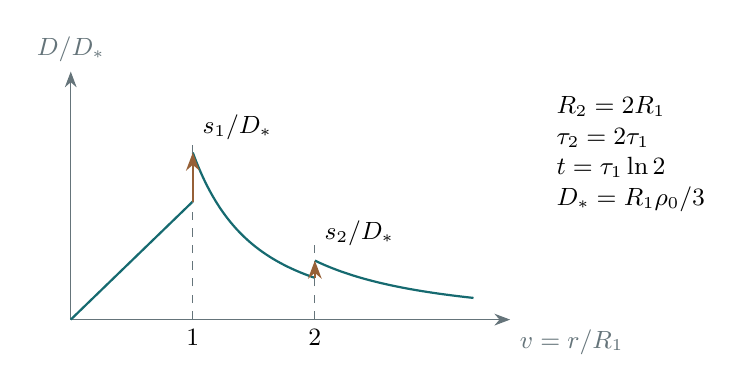
\begin{tikzpicture}[x=1.55cm,y=3cm,font=\small]
\draw[axis](0,0)--(3.6,0)node[below right]{$v=r/R_1$};\draw[axis](0,0)--(0,1.05)node[above]{$D/D_*$};
\draw[traj](0,0)--(1,.5);
\draw[traj,domain=1:2,samples=65,variable=\t]plot(\t,{sqrt(.5)/(\t*\t)});
\draw[traj,domain=2:3.3,samples=65,variable=\t]plot(\t,{1/(\t*\t)});
\draw[guide](1,0)--(1,.76);\draw[guide](2,0)--(2,.35);
\draw[force](1,.5)--(1,.707107);\draw[force](2,.176777)--(2,.25);
\node[above right]at(1,.72){$s_1/D_*$};\node[above right]at(2,.27){$s_2/D_*$};
\node[below]at(1,0){$1$};\node[below]at(2,0){$2$};
\node[right,align=left]at(3.9,.7){$R_2=2R_1$\\$\tau_2=2\tau_1$\\$t=\tau_1\ln2$\\$D_*=R_1\rho_0/3$};
\end{tikzpicture}
\figcaption{解图电4.4C　三段电位移的一个实际时刻。径向向外为正，两个向上跳变分别等于两界面的自由面电荷，外部场不随时间改变。}
\end{minipage}\end{center}

\Needspace{10\baselineskip}
解图电4.4C用同一时刻的三段D显示边界跳变。代入差指数后，中间段化为
\[
D=\frac{R_1^3\rho_0}{3r^2}e^{-t/\tau_2},
\]
其时间常数只剩$\tau_2$。
在$R_1$处右减左为$s_1$；在$R_2$处外减内为$s_2$。最外段与t无关，因为任何自由电荷都未穿过外边界；它也保证当内部场最终归零时，球外电场仍存在。
外表面的面电荷增长率等于内侧流向表面的电流密度：
\[
\dot s_2=j(R_2^-)=\frac{Q_0e^{-t/\tau_2}}{4\pi R_2^2\tau_2}.
\]
积分后与总电荷法一致。
两界面上的电荷分别由两侧的径向电流之差积累。把面密度乘相应球面积得到两面的电荷量，与内球的体电荷相加为初始总电荷。


\Needspace{13\baselineskip}

\pdfbookmark[2]{第 5 题 无碰撞双组分载流子的纵向小振动}{q5}

\section*{第 5 题\quad 无碰撞双组分载流子的纵向小振动}\label{q:5}

一均匀柱形介质的介电常量为$\varepsilon$，含正、负载流子，质量分别为$m_+,m_-$，电荷为$q_+>0,q_-<0$。平衡时两组分电荷体密度为$+\rho_0,-\rho_0$。温度足够低，可忽略热运动和碰撞阻尼。沿柱轴$x$有微小纵向扰动，使两组分发生电荷分离。在线性近似下证明该电荷分离模为简谐振动并求角频率；说明整体共同平移与此模的区别。

\begin{center}\begin{minipage}{.98\linewidth}\centering
\begin{tikzpicture}[scale=.9,transform shape]

\draw[object](0,0) rectangle(7,2.1);\foreach \x in {.5,1.5,2.5,3.5,4.5,5.5,6.5}{\node[color=accent] at(\x,1.4){$+$};\node[color=warm] at(\x,.6){$-$};}
\draw[axis](0,-.6)--(7.6,-.6) node[right]{$x$};\node[above] at(3.5,2.1){平衡：$+\rho_0,-\rho_0$};

\end{tikzpicture}
\figcaption{图电4.5\quad 两组分在同一介质中互相穿插，平衡时宏观电中性。}
\end{minipage}\end{center}

\Needspace{6\baselineskip}\subsection*{解答}

图电4.5中两组分稍作相反位移时，端部或局部密度起伏产生恢复电场。保留到扰动的一阶，电流密度为
\[
j=\rho_+v_++\rho_-v_-\simeq\rho_0(v_+-v_-).
\]
其中$\delta\rho_\pm v_\pm$为二阶小量，在线性化时略去。用解图电4.5A的薄片控制体写出
\[
\partial_t\rho=-\partial_xj,\qquad \partial_xE=\rho/\varepsilon,
\qquad m_\pm\partial_tv_\pm=q_\pm E.
\]

\begin{center}\begin{minipage}{.98\linewidth}\centering
\begin{tikzpicture}[scale=.9,transform shape]

\node[anchor=west] at(0,2.8){电荷分离模};\draw[guide](1,0)--(1,2.3);
\draw[motion](1,1.8)--(2.3,1.8) node[right]{$\xi_+$};\draw[force](1,1)--(.2,1) node[left]{$\xi_-$};
\draw[axis](2.1,.15)--(.2,.15) node[midway,below]{$E=-\rho_0\xi/\varepsilon$};
\node[anchor=west] at(5,2.8){共同平移};\draw[guide](5.5,.7)--(5.5,2.3);
\draw[motion](5.5,1.8)--(7,1.8) node[right]{$\xi_+$};\draw[force](5.5,1)--(7,1) node[right]{$\xi_-$};
\node at(6.5,0){$\xi=0,\quad\ddot X=0$};
\draw[object](3,-2.5) rectangle(4,-1.5);\draw[motion](1.6,-2)--(2.8,-2) node[midway,above]{$j(x)$};\draw[motion](4.2,-2)--(5.5,-2) node[midway,above]{$j(x+\dd x)$};
\draw[<->](3,-2.9)--(4,-2.9) node[midway,below]{$\dd x$};\draw[axis](5.8,-2)--(7.2,-2) node[right]{$x$};

\end{tikzpicture}
\figcaption{解图电4.5A\quad 相对位移产生恢复电场；共同平移不产生电荷分离，是不同的自由模。}
\end{minipage}\end{center}

对电流式求时间导数，再用两个动力学方程：
\[
\partial_tj=\rho_0\left(\frac{q_+}{m_+}-\frac{q_-}{m_-}\right)E.
\]
对连续性方程再求一次时间导数，并对上式作空间导数，得到
\[
\partial_t^2\rho=-\rho_0\left(\frac{q_+}{m_+}-\frac{q_-}{m_-}\right)\partial_xE
=-\frac{\rho_0}{\varepsilon}\left(\frac{q_+}{m_+}-\frac{q_-}{m_-}\right)\rho.
\]
所以电荷分离的角频率为
\[
\boxed{\omega_p=\sqrt{\frac{\rho_0}{\varepsilon}\left(\frac{q_+}{m_+}-\frac{q_-}{m_-}\right)}}.
\]
$q_-<0$，括号实际是两个正贡献之和，因此 $\omega_p^2>0$，密度扰动随时间作振动。密度扰动可写为$\rho(x,t)=A(x)\cos\omega_pt+B(x)\sin\omega_pt$，幅函数还需满足初始及边界条件。

解图电4.5A的两端面给出均匀位移的恢复场。令 $\xi=\xi_+-\xi_-$。取两组分重合时的场为零，$\xi>0$ 使右端出现正面电荷 $\rho_0\xi$，左端出现负面电荷 $-\rho_0\xi$。在一维平面模型中，两端面的场叠加为 $E=-\rho_0\xi/\varepsilon$，于是
\[
\ddot\xi=\left(\frac{q_+}{m_+}-\frac{q_-}{m_-}\right)E=-\omega_p^2\xi.
\]
该电场方向使正载流子向后、负载流子向前，减小分离。两质量密度分别为$\mu_\pm=\rho_0m_\pm/|q_\pm|$，总质心满足
\[
(\mu_++\mu_-)\ddot X=(\rho_0-\rho_0)E=0.
\]
所以共同平移满足 $X=X_0+V_0t$。相对振动叠加在这一匀速运动上；用随质心移动的坐标描述时，两组分各以同一频率振动。


解图电4.5A下方薄片还能把局部方程的符号写得更明确。截面积S、长度$\dd x$内的电荷变化为
\[
[\rho(x,t+\dd t)-\rho(x,t)]S\dd x=[j(x,t)-j(x+\dd x,t)]S\dd t.
\]
流入大于流出才使正电荷增加；约去共同因子并取极限，才得到$\partial_t\rho=-\partial_xj$。
同一薄片的左右电通量差为$[E(x+\dd x)-E(x)]S=\rho S\dd x/\varepsilon$，给出高斯定律。两式均以向右为正，负组分的符号已计入带符号电荷密度。

求导时的完整电流表达式是
\[
\partial_tj=\rho_+\partial_tv_++\rho_-\partial_tv_-+
(\partial_t\rho_+)v_++(\partial_t\rho_-)v_-.
\]
平衡速度为零，$v_\pm,\delta\rho_\pm$均为一阶扰动，最后两项为二阶；前两项中的$\rho_\pm$可取$\pm\rho_0$，其修正再乘一阶加速度也是二阶。
动力学中完整的物质加速度还可含$v_\pm\partial_xv_\pm$，它在同一线性近似下亦为二阶。这里忽略碰撞、压强和热运动，才得到所用的冷流体方程。

若沿电场路线计算，连续性与高斯定律只能先推出
\[
\partial_x(\varepsilon\partial_tE+j)=0,\qquad
\varepsilon\partial_tE+j=C(t).
\]
函数 $C(t)$ 是空间均匀的总电流密度，由端部与外部驱动条件确定。
在没有外加总电流的平面电荷分离模中取$C=0$，再求时间导数得到$\varepsilon\ddot E=-\dot j$，结合动力学也给$\ddot E+\omega_p^2E=0$。
对于沿轴整体均匀的相对位移，体内$\rho$可为零，恢复场由两端面电荷产生，在这一均匀模中，由端面带电量及几何条件确定场幅。
均匀相对位移的端部恢复场采用平面近似，局部体电荷的振动采用一维纵向方程。若端部场有显著的横向变化，均匀位移的恢复力需按实际几何求出。
\begin{center}\begin{minipage}{.97\linewidth}\centering
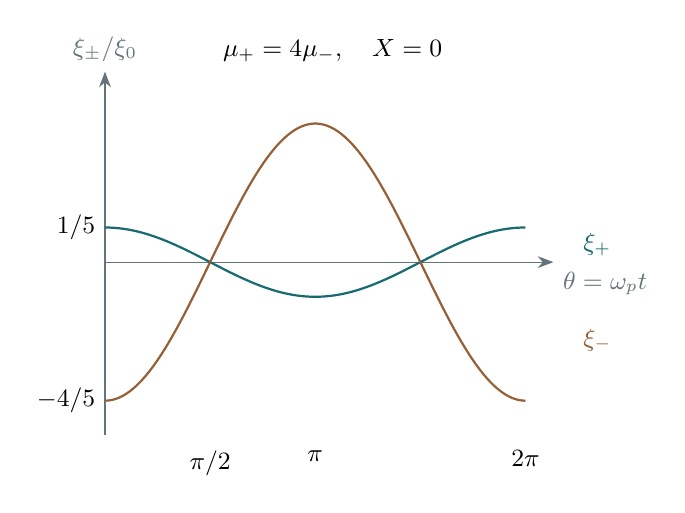
\begin{tikzpicture}[x=.85cm,y=2.2cm,font=\small]
\draw[axis](0,0)--(6.7,0)node[below right]{$\theta=\omega_pt$};\draw[axis](0,-1)--(0,1.1)node[above]{$\xi_\pm/\xi_0$};
\draw[traj,domain=0:6.283185,samples=120,variable=\t]plot(\t,{.2*cos(\t r)});
\draw[thick,warm,domain=0:6.283185,samples=120,variable=\t]plot(\t,{-.8*cos(\t r)});
\node[below]at(1.570796,-1.03){$\pi/2$};\node[below]at(3.141593,-1.03){$\pi$};\node[below]at(6.283185,-1.03){$2\pi$};
\node[left]at(0,.2){$1/5$};\node[left]at(0,-.8){$-4/5$};
\node[right,accent]at(7,.1){$\xi_+$};\node[right,warm]at(7,-.45){$\xi_-$};
\node[above]at(3.4,1.1){$\mu_+=4\mu_-,\quad X=0$};
\end{tikzpicture}
\figcaption{解图电4.5B　质量密度不等时的纯相对振动。两组分位移反相、幅度不同，质量加权中心保持不动；相对位移幅值为$\xi_0$。}
\end{minipage}\end{center}

解图电4.5B将两个粒子群的位移和质心分开。对纯相对模取$X=0$，联立$\mu_+\xi_++\mu_-\xi_-=0$与$\xi=\xi_+-\xi_-$，得
\[
\xi_+=\frac{\mu_-}{\mu_++\mu_-}\xi,\qquad
\xi_-=-\frac{\mu_+}{\mu_++\mu_-}\xi.
\]
所以两组分反相，但只有质量密度相同时振幅才相等。B图取$\mu_+=4\mu_-$，正组分振幅为相对振幅的1/5，负组分为4/5；按质量密度加权的中心在每一时刻都不动。
对一般初值，两式右边各加同一个 $X=X_0+V_0t$。取两式之差便消去共同平移，余下电荷分离位移 $\xi$。
\begin{center}\begin{minipage}{.97\linewidth}\centering
\begin{tikzpicture}[x=.85cm,y=2.5cm,font=\small]
\draw[axis](0,0)--(6.7,0)node[below right]{$\theta=\omega_pt$};\draw[axis](0,0)--(0,1.3)node[above]{能量比例};
\draw[traj,domain=0:6.283185,samples=140,variable=\t]plot(\t,{cos(\t r)^2});
\draw[thick,warm,domain=0:6.283185,samples=140,variable=\t]plot(\t,{sin(\t r)^2});
\draw[guide](0,1)--(6.3,1);\node[left]at(0,1){$1$};
\node[below]at(1.570796,0){$\pi/2$};\node[below]at(3.141593,0){$\pi$};\node[below]at(6.283185,0){$2\pi$};
\node[right,accent]at(7,1){$u_E/u_0$};\node[right,warm]at(7,.55){$u_K/u_0$};\node[right]at(7,.1){$u_E+u_K=u_0$};
\end{tikzpicture}
\figcaption{解图电4.5C　以初速度为零的纯相对模为例，场能与相对动能周期交换；频率相同的两组分共同承担相对动能。}
\end{minipage}\end{center}

解图电4.5C显示相对动能和电场能随时间的交换。定义约化质量密度$\mu_r=\mu_+\mu_-/(\mu_++\mu_-)$，则
\[
u_K=\frac12\mu_r\dot\xi^2,\qquad
u_E=\frac12\varepsilon E^2=\frac{\rho_0^2}{2\varepsilon}\xi^2,\qquad
\omega_p^2=\frac{\rho_0^2}{\varepsilon\mu_r}.
\]
由$1/\mu_r=1/\mu_++1/\mu_-$代回，最后一式正好等于两个荷质比之和给出的频率平方。
取$\xi=\xi_0\cos\omega_pt$，令$u_0=\rho_0^2\xi_0^2/(2\varepsilon)$，便有$u_E/u_0=\cos^2\omega_pt$、$u_K/u_0=\sin^2\omega_pt$。
场对两组分做功的总功率$jE=\rho_0\dot\xi E=-\dd u_E/\dd t$，与动能增加相抵，电场减少的能量恰成为相对动能。
共同平移若存在，还需加常量$\tfrac12(\mu_++\mu_-)V_0^2$，它不参与C图的周期能量交换。


\Needspace{13\baselineskip}

\pdfbookmark[2]{第 6 题 增加两个相同电阻能否保持端口电阻}{q6}

\section*{第 6 题\quad 增加两个相同电阻能否保持端口电阻}\label{q:6}

有限个阻值均为$r>0$的电阻构成二端网络，等效电阻为$R>0$。把该网络视为只可使用其两个端口的元件，在端口外以串、并联方式接入另两个阻值为$r$的电阻，两个新增电阻均须有效接入。能否使新的二端等效电阻仍等于$R$？

\begin{center}\begin{minipage}{.98\linewidth}\centering
\begin{tikzpicture}[scale=.9,transform shape]

\draw[object](0,0)--(1,0);\draw[object](1,-.6) rectangle(3,.6);\node at(2,0){有限网络$R$};\draw[object](3,0)--(4,0);
\fill(0,0) circle(2pt) node[left]{$A$};\fill(4,0) circle(2pt) node[right]{$B$};
\draw[object](5.5,-.35) rectangle(6.5,.35);\node at(6,0){$r$};\draw[object](8,-.35) rectangle(9,.35);\node at(8.5,0){$r$};
\node at(7.2,1){待接入的两个电阻};\node at(2,-1.2){仅使用$A,B$两个端口};

\end{tikzpicture}
\figcaption{图电4.6\quad 既有网络作为二端元件，新增电阻仅在端口之外连接。}
\end{minipage}\end{center}

\Needspace{6\baselineskip}\subsection*{解答}

图电4.6把既有网络作为电阻为$R$的二端元件。三个元件构成的串并联网络，交换两个相同的$r$后只有解图电4.6A中的六类；图中仅使用既有网络的两个端口，两个新增电阻均承载非零电流。

\begin{center}\begin{minipage}{.98\linewidth}\centering
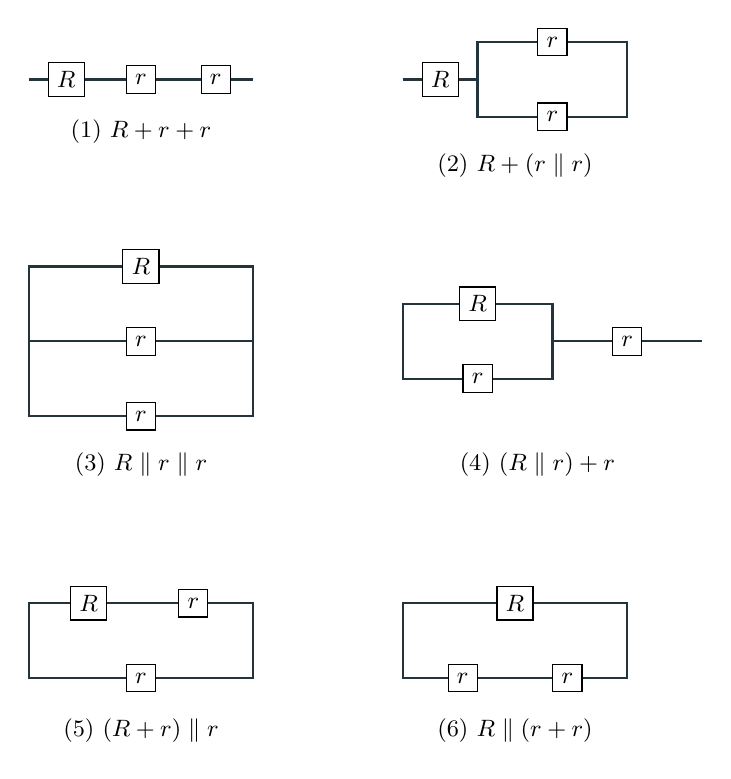
\begin{tikzpicture}[scale=.95,transform shape]

\begin{scope}[yshift=3.5cm]
\draw[object](0,0)--(3,0);\foreach \x/\s in {.5/R,1.5/r,2.5/r}{\node[draw,fill=white] at(\x,0){$\s$};}\node at(1.5,-.7){(1) $R+r+r$};
\draw[object](5,0)--(6,0)--(6,.5)--(8,.5)--(8,0)--(8,-.5)--(6,-.5)--(6,0);\node[draw,fill=white] at(5.5,0){$R$};\node[draw,fill=white] at(7,.5){$r$};\node[draw,fill=white] at(7,-.5){$r$};\node at(6.5,-1.15){(2) $R+(r\parallel r)$};
\end{scope}
\draw[object](0,0)--(0,1)--(3,1)--(3,0)--(3,-1)--(0,-1)--(0,0)--(3,0);\foreach \y/\s in {1/R,0/r,-1/r}{\node[draw,fill=white] at(1.5,\y){$\s$};}\node at(1.5,-1.65){(3) $R\parallel r\parallel r$};
\draw[object](5,0)--(5,.5)--(7,.5)--(7,-.5)--(5,-.5)--(5,0) (7,0)--(9,0);\node[draw,fill=white] at(6,.5){$R$};\node[draw,fill=white] at(6,-.5){$r$};\node[draw,fill=white] at(8,0){$r$};\node at(6.8,-1.65){(4) $(R\parallel r)+r$};
\begin{scope}[yshift=-4cm]
\draw[object](0,0)--(0,.5)--(3,.5)--(3,-.5)--(0,-.5)--cycle;\node[draw,fill=white] at(.8,.5){$R$};\node[draw,fill=white] at(2.2,.5){$r$};\node[draw,fill=white] at(1.5,-.5){$r$};\node at(1.5,-1.2){(5) $(R+r)\parallel r$};
\draw[object](5,0)--(5,.5)--(8,.5)--(8,-.5)--(5,-.5)--cycle;\node[draw,fill=white] at(6.5,.5){$R$};\node[draw,fill=white] at(5.8,-.5){$r$};\node[draw,fill=white] at(7.2,-.5){$r$};\node at(6.5,-1.2){(6) $R\parallel(r+r)$};
\end{scope}

\end{tikzpicture}
\figcaption{解图电4.6A\quad 六种串并联连接按两个相同$r$电阻的交换对称去重；各式对应同排电路。}
\end{minipage}\end{center}

按解图电4.6A从左至右、从上至下计算：
\[
\begin{aligned}
R_1&=R+2r,&R_2&=R+\frac r2,&R_3&=\frac{Rr}{2R+r},\\
R_4&=r+\frac{Rr}{R+r},&R_5&=\frac{r(R+r)}{R+2r},&R_6&=\frac{2Rr}{R+2r}.
\end{aligned}
\]
第1、2类在 $R$ 外增加串联电阻，所以结果较大。第3、6类在 $R$ 两端增加并联通路，所以结果较小。对第四种令$R_4=R$，乘$R+r$并整理：
\[
r(R+r)+Rr=R(R+r)\quad\Longrightarrow\quad R^2-Rr-r^2=0,
\]
所以正根为$R/r=(1+\sqrt5)/2$。第五种则给
\[
r(R+r)=R(R+2r)\quad\Longrightarrow\quad R^2+Rr-r^2=0,
\]
正根为$R/r=(\sqrt5-1)/2$。这两个条件本身允许正电阻，却都要求无理数比值。

还须使用“$R$由有限个相同电阻组成”的条件。把各节点电势以端口电压归一化，基尔霍夫方程的系数均为整数，消元所得节点电势和端口电流系数均为有理数。因此任何这样的有限网络都有
\[
\frac Rr\in\mathbb Q.
\]
这与两种根式条件矛盾，故\boxed{\text{在上述端口串并联条件下不能保持阻值不变。}}

若解除有限性，某些无限梯形网络恰有黄金比阻值，添加一节后可以保持不变；若允许进入已有网络的内部等势点，则还可能加上无电流支路。本题的六种连接以既有网络有限、只开放两个端口以及新增支路有效为条件。

\begin{center}\begin{minipage}{.97\linewidth}\centering
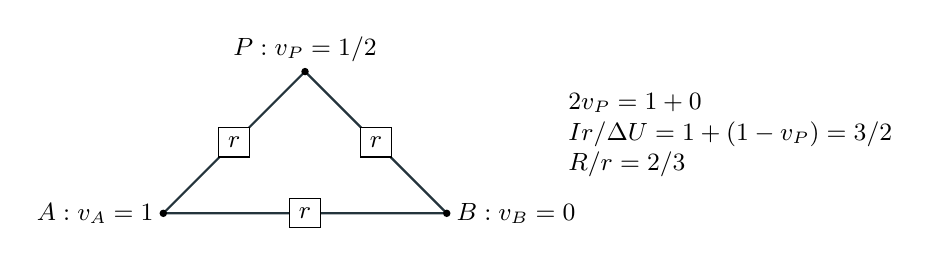
\begin{tikzpicture}[scale=.9,font=\small]
\draw[object](0,0)--(2,2)--(4,0)--cycle;
\node[draw,fill=white]at(1,1){$r$};\node[draw,fill=white]at(3,1){$r$};\node[draw,fill=white]at(2,0){$r$};
\fill(0,0)circle(1.5pt)node[left]{$A:v_A=1$};\fill(4,0)circle(1.5pt)node[right]{$B:v_B=0$};
\fill(2,2)circle(1.5pt)node[above]{$P:v_P=1/2$};
\node[align=left]at(8,1.1){$2v_P=1+0$\\$Ir/\Delta U=1+(1-v_P)=3/2$\\$R/r=2/3$};
\end{tikzpicture}
\figcaption{解图电4.6B　有限相同电阻网络的一个节点计算示例。单位端电压下先求内部有理电势，再求有理端口电导。}
\end{minipage}\end{center}

解图电4.6B以一个有限三角网络说明节点法的两步。令$v=V/\Delta U$，内部P点满足$(v_P-1)+(v_P-0)=0$，得$v_P=1/2$。
A端电流包括直接支路$\Delta U/r$与经P支路$\Delta U/(2r)$，所以$Ir/\Delta U=3/2$、$R/r=2/3$。
把解图电4.6B的内部节点方程推广到任意有限网络。对每个内部节点列$\sum_j(v_i-v_j)=0$，多条相同电阻边只使整数系数相加。
固定两端电势后，与端口相连部分的约化节点矩阵可逆；克拉默法则或有限高斯消元给有理节点电势。再把端口各支路的有理电流相加，得到非零有理电导，其倒数仍为有理数。
\begin{center}\begin{minipage}{.97\linewidth}\centering
\begin{tikzpicture}[x=2cm,y=1.7cm,font=\small]
\draw[axis](0,0)--(2.5,0)node[below right]{$x=R/r$};\draw[axis](0,0)--(0,2.6)node[above]{$R_{\text{新}}/r$};
\draw[guide](0,0)--(2.3,2.3);
\draw[traj,domain=0:2.3,samples=80,variable=\t]plot(\t,{1+\t/(1+\t)});
\draw[thick,warm,domain=0:2.3,samples=80,variable=\t]plot(\t,{(\t+1)/(\t+2)});
\fill(1.618034,1.618034)circle(1.5pt);\fill(.618034,.618034)circle(1.5pt);
\node[above left]at(1.618034,1.618034){$\varphi$};\node[below right]at(.618034,.618034){$1/\varphi$};
\node[right,accent]at(2.7,2){第(4)类：$1+x/(1+x)$};\node[right,warm]at(2.7,1.2){第(5)类：$(1+x)/(2+x)$};
\node[right]at(2.7,.45){虚线：保持条件$y=x$};
\end{tikzpicture}
\figcaption{解图电4.6C　两种混合连接的实际函数与保持直线。两处交点的横坐标是两种接法的正固定点。}
\end{minipage}\end{center}

解图电4.6C比较两种混合连接的增量。
第(4)类先并联再串联，增减可以抵消；第(5)类也有正的固定点。令$x=R/r$，两种增量分别为
\[
\frac{R_4-R}{r}=\frac{1+x-x^2}{1+x},\qquad
\frac{R_5-R}{r}=\frac{1-x-x^2}{2+x}.
\]
分母在$x>0$始终为正，故交点两侧确有增减方向变化。有限同值电阻网络的 $x$ 是有理数，因而实际可取点位于这两个无理数的两侧。
六类枚举的完整性来自三个二端元件的串并联构造：最外一步若为串联，内侧剩两元件可串或并；最外一步若为并联，内侧可并或串。再按哪个位置放R及两个r可交换去重，恰得解图电4.6A所列六类。


\Needspace{13\baselineskip}

\pdfbookmark[2]{第 7 题 由三个端口测量反推六只电阻}{q7}

\section*{第 7 题\quad 由三个端口测量反推六只电阻}\label{q:7}

图电4.7中，$a,b,c$分别为端点$X,Y,Z$的外接电阻，内部三角形的$X$侧至$Y$侧、$Y$侧至$Z$侧、$Z$侧至$X$侧分别为$f,d,e$。六只电阻恰为$1,2,3,4,5,6\,\Omega$各一只。第三端悬空时测得
\[
R_{XY}=7\frac3{13}\,\Omega,\quad R_{YZ}=10\frac1{13}\,\Omega,\quad R_{ZX}=6\frac9{13}\,\Omega.
\]
求$a,b,c,d,e,f$各自的阻值。

\begin{center}\begin{minipage}{.98\linewidth}\centering
\begin{tikzpicture}[scale=.9,transform shape]

\coordinate(X) at(0,2.5);\coordinate(Y) at(6,2.5);\coordinate(Z) at(3,-2);
\coordinate(P) at(1.5,1.3);\coordinate(Q) at(4.5,1.3);\coordinate(T) at(3,-.7);
\draw[object](X)--(P) (Y)--(Q) (Z)--(T) (P)--(Q)--(T)--cycle;
\foreach \p/\s in {X/X,Y/Y}{\fill(\p) circle(1.5pt) node[above]{$\s$};}
\fill(Z)circle(1.5pt)node[below]{$Z$};
\node[fill=white] at(.75,1.9){$a$};\node[fill=white] at(5.25,1.9){$b$};\node[fill=white] at(3,-1.35){$c$};
\node[fill=white] at(3,1.3){$f$};\node[fill=white] at(3.75,.3){$d$};\node[fill=white] at(2.25,.3){$e$};

\end{tikzpicture}
\figcaption{图电4.7\quad 外接三只电阻与内部三角形的标签固定，第三端在各次测量时悬空。}
\end{minipage}\end{center}

\Needspace{6\baselineskip}\subsection*{解答}

测 $X,Y$ 时，图电4.7的外侧电阻 $a,b$ 在被测通路上，$c$ 支路悬空。内部一边为 $f$，另一边经 $e,d$ 串联，两条内部通路并联。令$D=d+e+f$，三个方程为
\[
R_{XY}=a+b+\frac{f(e+d)}D,\quad
R_{YZ}=b+c+\frac{d(f+e)}D,\quad
R_{ZX}=c+a+\frac{e(d+f)}D.
\]

\begin{center}\begin{minipage}{.98\linewidth}\centering
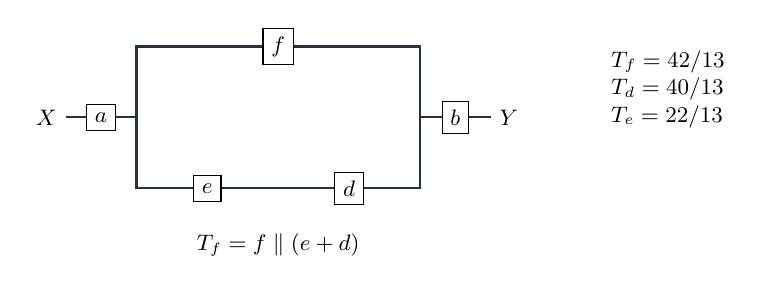
\begin{tikzpicture}[scale=.9,transform shape]

\draw[object](0,0)--(1,0)--(1,1)--(5,1)--(5,0)--(6,0) (1,0)--(1,-1)--(5,-1)--(5,0);
\node[draw,fill=white] at(.5,0){$a$};\node[draw,fill=white] at(5.5,0){$b$};
\node[draw,fill=white] at(3,1){$f$};\node[draw,fill=white] at(2,-1){$e$};\node[draw,fill=white] at(4,-1){$d$};
\node[left] at(0,0){$X$};\node[right] at(6,0){$Y$};\node at(3,-1.8){$T_f=f\parallel(e+d)$};
\node[align=left] at(8.5,.4){$T_f=42/13$\\$T_d=40/13$\\$T_e=22/13$};

\end{tikzpicture}
\figcaption{解图电4.7A\quad 测量$X,Y$时内部两条路径并联；右侧列出确定后的三个内部等效项（单位为欧姆）。}
\end{minipage}\end{center}

解图电4.7A把这些分式分别记为$T_f,T_d,T_e$。六只电阻均取整数欧姆，而测量含不可约分母13，所以这些分式的分母$D$必须含因子13。三只不同电阻之和在6至15之间，故
\[
D=13\,\Omega,\qquad\{d,e,f\}=\{3,4,6\}\ \text{或}\ \{2,5,6\}.
\]
若取$\{3,4,6\}$，三个分式为$30/13,36/13,42/13$，小数部分为$4/13,10/13,3/13$，不能与测量中的$3/13,1/13,9/13$匹配。因此只剩$\{2,5,6\}$。

这一组中，各阻值与其分式的对应为
\[
2\longmapsto\frac{22}{13}=1\frac9{13},\quad
5\longmapsto\frac{40}{13}=3\frac1{13},\quad
6\longmapsto\frac{42}{13}=3\frac3{13}.
\]
由测量的小数部分逐项对应，得$e=2\,\Omega,d=5\,\Omega,f=6\,\Omega$。从三次测量中分别减去内部等效项：
\[
a+b=4,\qquad b+c=7,\qquad c+a=5\quad(\Omega).
\]
相加及相减给
\[
\boxed{a=1,\ b=3,\ c=4,\ d=5,\ e=2,\ f=6\quad(\Omega)}.
\]
回代第一式为$1+3+42/13=94/13\,\Omega$，第二式为$3+4+40/13=131/13\,\Omega$，第三式为$4+1+22/13=87/13\,\Omega$，均与测量相符。三个端口值先确定三个总星臂。利用题给的六个离散值各用一次，逐项匹配内部三角形后才得到六条支路。


分母筛选还可补上可约分的判断。将阻值以$\Omega$为单位写成整数，则$T_f=f(D-f)/D$的约分后分母必须整除D；外接整数$a+b$不会改变其分数部分。
既然$R_{XY}$的最简分母是13，就有$13\mid D$，而三只不同阻值的最小和为$1+2+3=6$、最大和为$4+5+6=15$，所以唯一可能的13倍数是13。
整除条件给 $D$ 的候选倍数，六个给定阻值则把候选限制到该区间内唯一的13。

对保留的$\{2,5,6\}$，也可不直接猜标签，而逐个列整数乘积。$T_e$的分数部分为$9/13$，故$e(13-e)$在$22,40,42$中只能为22，得到$e=2$。
继而$T_d$对应$1/13$，取$d(13-d)=40$得到$d=5$，剩下$f=6$。
外接的三条两两和给$a=[(a+b)+(a+c)-(b+c)]/2=(4+5-7)/2=1$，另两只同理得到3和4；这明确了从分数部分到整数部分的每一步。
\begin{center}\begin{minipage}{.97\linewidth}\centering
\begin{tikzpicture}[scale=.85,font=\small]
\draw[object](0,2)--(3,0)--(6,2) (3,0)--(3,-2.5);
\node[draw,fill=white]at(1.5,1){$A_X$};\node[draw,fill=white]at(4.5,1){$A_Y$};\node[draw,fill=white]at(3,-1.3){$A_Z$};
\fill(0,2)circle(1.5pt)node[above]{$X$};\fill(6,2)circle(1.5pt)node[above]{$Y$};\fill(3,-2.5)circle(1.5pt)node[below]{$Z$};\fill(3,0)circle(1.5pt)node[right]{$O$};
\node[right,align=left]at(7,.2){$A_X=a+ef/D=25/13$\\$A_Y=b+df/D=69/13$\\$A_Z=c+de/D=62/13$\\单位：$\Omega$};
\end{tikzpicture}
\figcaption{解图电4.7B　全网络的三端星形等效。测量确定三条总星臂，但每条总星臂内部如何拆分，还需六只电阻的离散条件。}
\end{minipage}\end{center}

解图电4.7B将三个测量值写成总星臂的加和。将内部三角形换成星形，靠近X、Y、Z的内星臂分别为$ef/D,df/D,de/D$，再分别与a、b、c串联。
于是三个总星臂可直接从测量求得
\[
A_X=\frac{R_{XY}+R_{ZX}-R_{YZ}}2=\frac{25}{13}\,\Omega,\quad
A_Y=\frac{R_{XY}+R_{YZ}-R_{ZX}}2=\frac{69}{13}\,\Omega,
\]
\[
A_Z=\frac{R_{YZ}+R_{ZX}-R_{XY}}2=\frac{62}{13}\,\Omega.
\]
代入已求阻值，三条内星臂分别为$12/13,30/13,10/13\,\Omega$，与外接1、3、4相加恰好得到B图所标结果。
若阻值允许连续变化，三次测量只确定这三个总星臂；每臂由外接电阻和内星臂构成的分配仍可变化，所以离散集合是唯一反演所必需的信息。
\begin{center}\begin{minipage}{.97\linewidth}\centering
\begin{tikzpicture}[scale=.9,font=\small]
\draw[object](0,0)--(1,0)--(1,1)--(5,1)--(5,0)--(6,0) (1,0)--(1,-1)--(5,-1)--(5,0);
\node[draw,fill=white]at(.5,0){$1$};\node[draw,fill=white]at(5.5,0){$3$};\node[draw,fill=white]at(3,1){$6$};\node[draw,fill=white]at(2,-1){$2$};\node[draw,fill=white]at(4,-1){$5$};
\draw[motion](1.5,1.55)--(4.5,1.55)node[midway,above]{$7I_0/13$};
\draw[motion](1.5,-1.55)--(4.5,-1.55)node[midway,below]{$6I_0/13$};
\node[left]at(0,0){$X$};\node[right]at(6,0){$Y$};\node[right,align=left]at(7,.2){电阻单位：$\Omega$\\$I_0=1\,\mathrm A$\\$U_{XY}=94/13\,\mathrm V$};
\end{tikzpicture}
\figcaption{解图电4.7C　确定阻值后的$X,Y$测量回路。两内部支路分流之和等于端口电流，第三端外接电阻仍无电流。}
\end{minipage}\end{center}

\Needspace{8\baselineskip}
解图电4.7C以测量 $X,Y$ 为例，画出并联通路上的实际分流。内部直接支路为$6\,\Omega$，绕经下方的支路为$2+5=7\,\Omega$，并联等效为$42/13\,\Omega$。
取端口电流$I_0=1\,\mathrm A$，两支路分别为$7/13\,\mathrm A$与$6/13\,\mathrm A$，内部电压都为$42/13\,\mathrm V$；再加a、b上的1和3伏压降，端口电压为$94/13\,\mathrm V$。
第三端 $Z$ 悬空，故 $c$ 中电流为零。下方的 $d,e$ 仍组成一条通路，各有 $6/13\,\mathrm A$ 通过。


\Needspace{13\baselineskip}

\pdfbookmark[2]{第 8 题 三次测量识别八只电阻中的异值者}{q8}

\section*{第 8 题\quad 三次测量识别八只电阻中的异值者}\label{q:8}

有八只外观相同的正电阻，其中七只阻值相同，另一只阻值不同，但不知道正常值及异常值，也不知道异常电阻较大还是较小。只使用理想欧姆表测量三次，设计可唯一识别异常电阻的接线与判断方案。

\begin{center}\begin{minipage}{.98\linewidth}\centering
\begin{tikzpicture}[scale=.9,transform shape]

\foreach \i in {1,...,8}{\pgfmathsetmacro{\xx}{mod(\i-1,4)*2.4}\pgfmathsetmacro{\yy}{-floor((\i-1)/4)*1.7}
\draw[object](\xx,\yy)--++(.4,0);\node[draw,minimum width=11mm,minimum height=4mm,anchor=west] at(\xx+.4,\yy){$R_\i$};\draw[object](\xx+1.5,\yy)--++(.4,0);}
\node at(4.7,1){七只同值，一只异值；正常值也未知};

\end{tikzpicture}
\figcaption{图电4.8\quad 先给八只外观相同的电阻编号，测量接线可随前两次结果调整。}
\end{minipage}\end{center}

\Needspace{6\baselineskip}\subsection*{解答}

先给八只电阻编号$R_1,\ldots,R_8$。解图电4.8B的前两次测量分别把$R_1,R_2,R_3$串联得到$A$，把$R_4,R_5,R_6$串联得到$B$。

\begin{center}\begin{minipage}{.97\linewidth}\centering
\begin{tikzpicture}[scale=.85,font=\small]
\draw[object](0,1.2)--(6,1.2) (0,-1.2)--(6,-1.2);
\foreach \x/\a/\b in {1/1/4,3/2/5,5/3/6}{\node[draw,fill=white]at(\x,1.2){$R_\a$};\node[draw,fill=white]at(\x,-1.2){$R_\b$};}
\fill(0,1.2)circle(1.5pt);\fill(6,1.2)circle(1.5pt);\fill(0,-1.2)circle(1.5pt);\fill(6,-1.2)circle(1.5pt);
\node[left]at(0,1.2){第一次};\node[left]at(0,-1.2){第二次};
\node[right,align=left]at(7,1.2){$A=R_1+R_2+R_3$};\node[right,align=left]at(7,-1.2){$B=R_4+R_5+R_6$};
\node at(3,0){两次接线分别测量，互不连接};
\end{tikzpicture}
\figcaption{解图电4.8B　前两次串联测量。两组和不等时，7、8号才可作为正常辅助支路；交换两组编号须同步修改第三次接线标号。}
\end{minipage}\end{center}

若$A=B$，异常者只能在$R_7,R_8$中。第三次测$R_7$：若结果不等于$A/3$，则为$R_7$；相等则为$R_8$。因为只有一只异常，两个含三只电阻的组不可能同时产生相同的非正常改变量。

若$A\ne B$，交换两组三只的编号（必要时）使$A>B$，记$\alpha=A/B>1$。第三次按解图电4.8A接入全部八只，测量的网络为
\[
C=\bigl[R_1\parallel(R_2+(R_3\parallel R_7))\bigr]
+\bigl[R_4\parallel(R_5+(R_6\parallel R_8))\bigr].
\]

\begin{center}\begin{minipage}{.98\linewidth}\centering
\begin{tikzpicture}[scale=.85,transform shape]

\foreach \shift/\a/\b/\c/\d in {0/1/2/3/7,5.5/4/5/6/8}{\begin{scope}[xshift=\shift cm]
\draw[object](0,0)--(0,2)--(3.8,2)--(3.8,0)--cycle;
\draw[object](1.8,2)--(1.8,3.1)--(3.8,3.1)--(3.8,2);
\node[draw,fill=white] at(1.8,0){$R_\a$};\node[draw,fill=white] at(0,1){$R_\b$};
\node[draw,fill=white] at(2.8,2){$R_\c$};\node[draw,fill=white] at(2.8,3.1){$R_\d$};
\end{scope}}
\draw[object](3.8,0)--(5.5,0);\fill(0,0) circle(2pt) node[below left]{$C_1$};\fill(9.3,0) circle(2pt) node[below right]{$C_2$};
\node at(4.65,-.8){测$C_1,C_2$间总电阻$C$};

\end{tikzpicture}
\figcaption{解图电4.8A\quad 第三次测量的两个不对称模块串联；上方两只电阻并联后再与左竖支路串联。}
\end{minipage}\end{center}

由于异常者已确定在前六只中，$R_7,R_8$均正常。记三元模块
\[
g(x,y,z;R)=x\parallel\left(y+\frac{zR}{z+R}\right)
=\frac{x[y(z+R)+zR]}{x(z+R)+y(z+R)+zR}.
\]
三只都正常时$g(R,R,R;R)=3R/5$。若异常在第一组，则正常值$R=B/3$、异常值$r=A-2B/3=(3\alpha-2)R$；分别令$x,y,z$中的一项为$r$，得到前三种预测值。若异常在第二组，则$R=A/3$、$r=B-2A/3=(3/\alpha-2)R$，此分支还要求$1<\alpha<3/2$。按图中1至6号位置逐一代入，结果为
\[
\begin{array}{c|c}
\text{异常编号}&C/B\\\hline
1&(3\alpha-2)/(6\alpha-1)+1/5\\
2&(2\alpha-1)/(6\alpha-1)+1/5\\
3&(2\alpha-1)/(9\alpha-4)+1/5\\
4&\alpha[(3-2\alpha)/(6-\alpha)+1/5]\\
5&\alpha[(2-\alpha)/(6-\alpha)+1/5]\\
6&\alpha[(2-\alpha)/(9-4\alpha)+1/5].
\end{array}
\]
例如$R_1$异常时，左模块为$r\parallel(3R/2)=3Rr/(2r+3R)$，右模块为$3R/5$；除以$B=3R$便得到表中第一行，其余各行由同一模块式代入。

在$1<\alpha<3/2$内，这六个预测值严格满足
\[
C_6>C_1>C_5>C_2>C_3>C_4.
\]
为逐项证明可辨识，令$\Delta_{ij}=(C_i-C_j)/B$，五个相邻差为
\[
\begin{aligned}
\Delta_{61}&=\frac{9(\alpha-1)^2(11-6\alpha)}{5(9-4\alpha)(6\alpha-1)},\\
\Delta_{15}&=\frac{3(\alpha-1)(12\alpha^2-29\alpha+22)}{5(6-\alpha)(6\alpha-1)},\\
\Delta_{52}&=\frac{2(\alpha-1)(-18\alpha^2+41\alpha-18)}{5(6-\alpha)(6\alpha-1)},\\
\Delta_{23}&=\frac{3(\alpha-1)(2\alpha-1)}{(6\alpha-1)(9\alpha-4)},\\
\Delta_{34}&=\frac{9(\alpha-1)^2(11\alpha-6)}{5(6-\alpha)(9\alpha-4)}.
\end{aligned}
\]
区间$1<\alpha<3/2$内分母及一次因子均为正。第二式二次因子的判别式$29^2-4\cdot12\cdot22<0$且首项系数为正；第三式二次因子是凹函数，在区间两端的值分别为5和3，区间内也为正。故五个差均严格大于零，第三次实测$C$能与表中唯一一行匹配。若$\alpha\ge3/2$，后组三种会要求非正异常阻值，全部排除，只比较第一至三行；前两行有 $C_1>C_2$，因为同分母下的分子相差 $\alpha-1$。第二、三行的分子相同，第三行分母较大，故 $C_2>C_3$。方案共用三次测量，而且不依赖预先知道异常偏大或偏小。实际测量有误差时，异常值非常接近正常值会使各预测值接近，须另作仪器分辨率判断。

\begin{center}\begin{minipage}{.97\linewidth}\centering
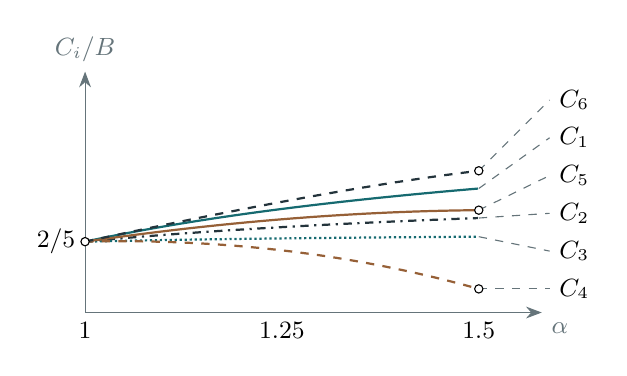
\begin{tikzpicture}[x=10cm,y=6cm,font=\small]
\draw[axis](0,.25)--(.58,.25)node[below right]{$\alpha$};\draw[axis](0,.25)--(0,.76)node[above]{$C_i/B$};
\draw[traj,domain=1:1.5,samples=110,variable=\t]plot({\t-1},{(3*\t-2)/(6*\t-1)+.2});
\draw[thick,ink,dash dot,domain=1:1.5,samples=110,variable=\t]plot({\t-1},{(2*\t-1)/(6*\t-1)+.2});
\draw[thick,accent,densely dotted,domain=1:1.5,samples=110,variable=\t]plot({\t-1},{(2*\t-1)/(9*\t-4)+.2});
\draw[thick,warm,dashed,domain=1:1.5,samples=110,variable=\t]plot({\t-1},{\t*((3-2*\t)/(6-\t)+.2)});
\draw[thick,warm,domain=1:1.5,samples=110,variable=\t]plot({\t-1},{\t*((2-\t)/(6-\t)+.2)});
\draw[thick,ink,dashed,domain=1:1.5,samples=110,variable=\t]plot({\t-1},{\t*((2-\t)/(9-4*\t)+.2)});
\draw[fill=white](0,.4)circle(1.5pt);\node[left]at(0,.4){$2/5$};
\node[below]at(0,.25){$1$};\node[below]at(.25,.25){$1.25$};\node[below]at(.5,.25){$1.5$};
\foreach \v/\labely/\i in {.55/.70/6,.5125/.62/1,.466667/.54/5,.45/.46/2,.410526/.38/3,.3/.30/4}{\draw[guide](.5,\v)--(.59,\labely);\node[right]at(.59,\labely){$C_\i$};}
\foreach \v in {.55,.466667,.3}{\draw[fill=white](.5,\v)circle(1.5pt);}
\end{tikzpicture}
\figcaption{解图电4.8C　六个预测值的实际曲线。$1<\alpha<1.5$时保持严格次序；$\alpha=1$的合并点及后组三分支在1.5处的边界用空心点表示，不作为正异值候选。}
\end{minipage}\end{center}

解图电4.8C将表中六个候选值画在同一尺度上。同样的 $A>B$ 可由第一组的偏大电阻造成，也可由第二组的偏小电阻造成。两种情形给出不同的正常阻值。
例如$A>B$但$A/B<3/2$时，两种正常值$B/3$与$A/3$都须保留。当 $A/B\ge3/2$，第二组假设给出 $r\le0$，所以只保留前三行。

第三次测量用解图电4.8A的同一套接线。六个数值来自把不同位置及阻值代入这一网络。
A图的两个模块互不跨接，左、右端分别接欧姆表，中点只连接两模块；B图两次串联测量则分别完成，没有把两组并成一个供测网络。
若交换前两组三只的编号使$A>B$，应记下新旧标签的对应；得出异常的工作编号后，再还原到那只实际元件。

还可说明理想可辨识与有限误差的差别。设$\delta=\alpha-1$很小，C图中最接近的若干候选在一阶变化上相同，例如
\[
\frac{C_6-C_1}{B}=\frac9{25}\delta^2+O(\delta^3),\qquad
\frac{C_3-C_4}{B}=\frac9{25}\delta^2+O(\delta^3).
\]
它们对任意非零正$\delta$仍不相等，但间距按二阶小量缩小。若前两次结果视为准确、第三次测量的绝对误差不超过$\eta$，要使所有候选误差区间互不重叠，充分条件为$\min_{i\ne j}|C_i-C_j|>2\eta$。
若前两次也有误差，用 $A,B$ 的允许范围计算各候选的预测区间，再与第三次的测量区间比较。


\Needspace{13\baselineskip}

\pdfbookmark[2]{第 9 题 细分正四面体电阻网的两类端口}{q9}

\section*{第 9 题\quad 细分正四面体电阻网的两类端口}\label{q:9}

正四面体四个顶点记为$A,B,P,Q$，六条棱的中点均为节点。把每条棱分成两段，并在每个三角形面内连接三条棱中点，形成图电4.9的框架网络。每一小段电阻均为$R$。令$C$为$AB$中点、$D$为其对棱$PQ$中点，求$R_{AB}$和$R_{CD}$。所有相交线只在标明的十个节点处电连接。

\begin{center}\begin{minipage}{.98\linewidth}\centering
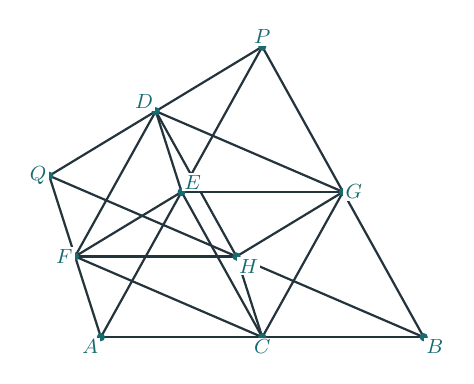
\begin{tikzpicture}[scale=.82,transform shape]
\coordinate (g0) at (0,0);
\coordinate (g1) at (5,0);
\coordinate (g2) at (2.5,4.5);
\coordinate (g3) at (-0.8,2.5);
\coordinate (g4) at (2.5,0);
\coordinate (g5) at (1.25,2.25);
\coordinate (g6) at (-0.4,1.25);
\coordinate (g7) at (3.75,2.25);
\coordinate (g8) at (2.1,1.25);
\coordinate (g9) at (0.85,3.5);
\draw[object] (g0)--(g4);
\draw[object] (g1)--(g4);
\draw[object] (g0)--(g5);
\draw[object] (g2)--(g5);
\draw[object] (g0)--(g6);
\draw[object] (g3)--(g6);
\draw[object] (g1)--(g7);
\draw[object] (g2)--(g7);
\draw[object] (g1)--(g8);
\draw[object] (g3)--(g8);
\draw[object] (g2)--(g9);
\draw[object] (g3)--(g9);
\draw[object] (g4)--(g5);
\draw[object] (g4)--(g6);
\draw[object] (g4)--(g7);
\draw[object] (g4)--(g8);
\draw[object] (g5)--(g6);
\draw[object] (g5)--(g7);
\draw[object] (g5)--(g9);
\draw[object] (g6)--(g8);
\draw[object] (g6)--(g9);
\draw[object] (g7)--(g8);
\draw[object] (g7)--(g9);
\draw[object] (g8)--(g9);
\fill[accent] (g0) circle(1.8pt) node[below left,fill=white,inner sep=1pt]{$A$};
\fill[accent] (g1) circle(1.8pt) node[below right,fill=white,inner sep=1pt]{$B$};
\fill[accent] (g2) circle(1.8pt) node[above,fill=white,inner sep=1pt]{$P$};
\fill[accent] (g3) circle(1.8pt) node[left,fill=white,inner sep=1pt]{$Q$};
\fill[accent] (g4) circle(1.8pt) node[below,fill=white,inner sep=1pt]{$C$};
\fill[accent] (g5) circle(1.8pt) node[above right,fill=white,inner sep=1pt]{$E$};
\fill[accent] (g6) circle(1.8pt) node[left,fill=white,inner sep=1pt]{$F$};
\fill[accent] (g7) circle(1.8pt) node[right,fill=white,inner sep=1pt]{$G$};
\fill[accent] (g8) circle(1.8pt) node[below right,fill=white,inner sep=1pt]{$H$};
\fill[accent] (g9) circle(1.8pt) node[above left,fill=white,inner sep=1pt]{$D$};
\end{tikzpicture}
\figcaption{图电4.9\quad 正四面体各面连接棱中点，每一小段均为$R$，只有十个实点是节点。}
\end{minipage}\end{center}

\Needspace{6\baselineskip}\subsection*{解答}

此网络共有4个顶点、6个棱中点及24条电阻边。图电4.9中，只有标点的十处连接导线。分别给两种端口加压，各自确定等势分组。

\begin{center}\begin{minipage}{.98\linewidth}\centering
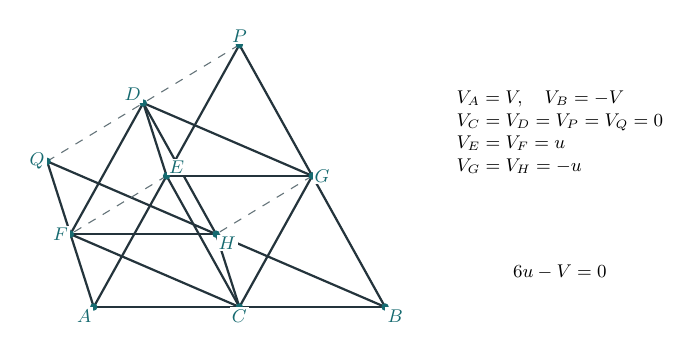
\begin{tikzpicture}[scale=.74,transform shape]
\coordinate (g0) at (0,0);
\coordinate (g1) at (5,0);
\coordinate (g2) at (2.5,4.5);
\coordinate (g3) at (-0.8,2.5);
\coordinate (g4) at (2.5,0);
\coordinate (g5) at (1.25,2.25);
\coordinate (g6) at (-0.4,1.25);
\coordinate (g7) at (3.75,2.25);
\coordinate (g8) at (2.1,1.25);
\coordinate (g9) at (0.85,3.5);
\draw[object] (g0)--(g4);
\draw[object] (g1)--(g4);
\draw[object] (g0)--(g5);
\draw[object] (g2)--(g5);
\draw[object] (g0)--(g6);
\draw[object] (g3)--(g6);
\draw[object] (g1)--(g7);
\draw[object] (g2)--(g7);
\draw[object] (g1)--(g8);
\draw[object] (g3)--(g8);
\draw[guide] (g2)--(g9);
\draw[guide] (g3)--(g9);
\draw[object] (g4)--(g5);
\draw[object] (g4)--(g6);
\draw[object] (g4)--(g7);
\draw[object] (g4)--(g8);
\draw[guide] (g5)--(g6);
\draw[object] (g5)--(g7);
\draw[object] (g5)--(g9);
\draw[object] (g6)--(g8);
\draw[object] (g6)--(g9);
\draw[guide] (g7)--(g8);
\draw[object] (g7)--(g9);
\draw[object] (g8)--(g9);
\fill[accent] (g0) circle(1.8pt) node[below left,fill=white,inner sep=1pt]{$A$};
\fill[accent] (g1) circle(1.8pt) node[below right,fill=white,inner sep=1pt]{$B$};
\fill[accent] (g2) circle(1.8pt) node[above,fill=white,inner sep=1pt]{$P$};
\fill[accent] (g3) circle(1.8pt) node[left,fill=white,inner sep=1pt]{$Q$};
\fill[accent] (g4) circle(1.8pt) node[below,fill=white,inner sep=1pt]{$C$};
\fill[accent] (g5) circle(1.8pt) node[above right,fill=white,inner sep=1pt]{$E$};
\fill[accent] (g6) circle(1.8pt) node[left,fill=white,inner sep=1pt]{$F$};
\fill[accent] (g7) circle(1.8pt) node[right,fill=white,inner sep=1pt]{$G$};
\fill[accent] (g8) circle(1.8pt) node[below right,fill=white,inner sep=1pt]{$H$};
\fill[accent] (g9) circle(1.8pt) node[above left,fill=white,inner sep=1pt]{$D$};
\node[align=left] at(8,3){$V_A=V,\quad V_B=-V$\\$V_C=V_D=V_P=V_Q=0$\\$V_E=V_F=u$\\$V_G=V_H=-u$};
\node at(8,.6){$6u-V=0$};

\end{tikzpicture}
\figcaption{解图电4.9A\quad 顶点$A,B$激励下的电势分组；虚线边在本次激励下电流为零；选$E$列六支路节点式。}
\end{minipage}\end{center}

\textbf{从$A$流入、$B$流出。}在解图电4.9A中取$V_A=V,V_B=-V$。交换$A,B$并使电势反号时网络不变，因此$C,D,P,Q$均为零电势。$AP,AQ$中点等势为$u$，$BP,BQ$中点为$-u$。以$AP$中点为例，它连接$A,P$及四个相邻棱中点，六条支路的节点方程为
\[
\frac1R[(u-V)+u+(u-u)+u+(u+u)+u]=0,
\qquad u=\frac V6.
\]
$A$点只有通向$C$及两个电势为$u$的中点的三支路，所以输入电流
\[
I=\frac{V+2(V-u)}R=\frac{8V}{3R},\qquad
\boxed{R_{AB}=\frac{2V}{I}=\frac34R}.
\]

\textbf{从$C$流入、$D$流出。}重新取$V_C=V,V_D=-V$。解图电4.9B中$A,B$等势为$p$，$P,Q$等势为$-p$，其余四个棱中点均为零。顶点$A$连接$C$及两个零势中点，有
\[
3p-V=0,\qquad p=\frac V3.
\]
$C$连接两个电势为$p$的顶点和四个零势中点，故
\[
I=\frac{2(V-p)+4V}R=\frac{16V}{3R},\qquad
\boxed{R_{CD}=\frac{2V}{I}=\frac38R}.
\]

\begin{center}\begin{minipage}{.98\linewidth}\centering
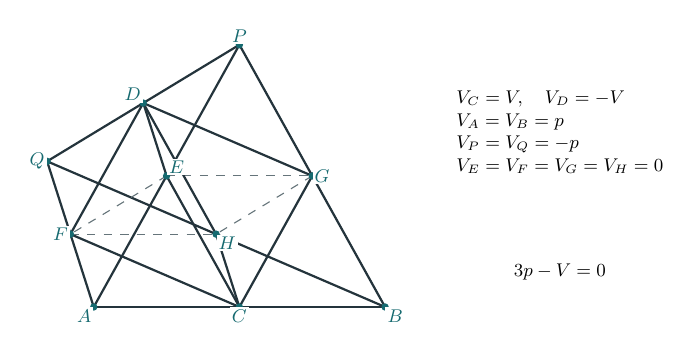
\begin{tikzpicture}[scale=.74,transform shape]
\coordinate (g0) at (0,0);
\coordinate (g1) at (5,0);
\coordinate (g2) at (2.5,4.5);
\coordinate (g3) at (-0.8,2.5);
\coordinate (g4) at (2.5,0);
\coordinate (g5) at (1.25,2.25);
\coordinate (g6) at (-0.4,1.25);
\coordinate (g7) at (3.75,2.25);
\coordinate (g8) at (2.1,1.25);
\coordinate (g9) at (0.85,3.5);
\draw[object] (g0)--(g4);
\draw[object] (g1)--(g4);
\draw[object] (g0)--(g5);
\draw[object] (g2)--(g5);
\draw[object] (g0)--(g6);
\draw[object] (g3)--(g6);
\draw[object] (g1)--(g7);
\draw[object] (g2)--(g7);
\draw[object] (g1)--(g8);
\draw[object] (g3)--(g8);
\draw[object] (g2)--(g9);
\draw[object] (g3)--(g9);
\draw[object] (g4)--(g5);
\draw[object] (g4)--(g6);
\draw[object] (g4)--(g7);
\draw[object] (g4)--(g8);
\draw[guide] (g5)--(g6);
\draw[guide] (g5)--(g7);
\draw[object] (g5)--(g9);
\draw[guide] (g6)--(g8);
\draw[object] (g6)--(g9);
\draw[guide] (g7)--(g8);
\draw[object] (g7)--(g9);
\draw[object] (g8)--(g9);
\fill[accent] (g0) circle(1.8pt) node[below left,fill=white,inner sep=1pt]{$A$};
\fill[accent] (g1) circle(1.8pt) node[below right,fill=white,inner sep=1pt]{$B$};
\fill[accent] (g2) circle(1.8pt) node[above,fill=white,inner sep=1pt]{$P$};
\fill[accent] (g3) circle(1.8pt) node[left,fill=white,inner sep=1pt]{$Q$};
\fill[accent] (g4) circle(1.8pt) node[below,fill=white,inner sep=1pt]{$C$};
\fill[accent] (g5) circle(1.8pt) node[above right,fill=white,inner sep=1pt]{$E$};
\fill[accent] (g6) circle(1.8pt) node[left,fill=white,inner sep=1pt]{$F$};
\fill[accent] (g7) circle(1.8pt) node[right,fill=white,inner sep=1pt]{$G$};
\fill[accent] (g8) circle(1.8pt) node[below right,fill=white,inner sep=1pt]{$H$};
\fill[accent] (g9) circle(1.8pt) node[above left,fill=white,inner sep=1pt]{$D$};
\node[align=left] at(8,3){$V_C=V,\quad V_D=-V$\\$V_A=V_B=p$\\$V_P=V_Q=-p$\\$V_E=V_F=V_G=V_H=0$};
\node at(8,.6){$3p-V=0$};

\end{tikzpicture}
\figcaption{解图电4.9B\quad 对棱中点$C,D$激励时重新分组；虚线四边无电流，顶点$A$的三支路决定$p$。}
\end{minipage}\end{center}

\begin{center}\begin{minipage}{.98\linewidth}\centering
\begin{tikzpicture}[scale=.9,transform shape]

\draw[object](0,0)--(0,2)--(5,2)--(5,0)--cycle;\node[draw,fill=white] at(2.5,0){$2R$};
\node[draw,fill=white] at(.6,2){$R/2$};\node[draw,fill=white] at(4.4,2){$R/2$};
\draw[object](1.3,2)--(1.3,3)--(3.7,3)--(3.7,2);\node[draw,fill=white] at(2.5,3){$R/4$};\node[draw,fill=white] at(2.5,2){$R$};
\node[below left] at(0,0){$A$};\node[below right] at(5,0){$B$};
\node at(2.5,4){$AB$端口的折叠网};
\draw[guide](1.3,2)--(1.3,1.7);\draw[guide](3.7,2)--(3.7,1.7);\node at(1.3,1.4){$E=F$};\node at(3.7,1.4){$G=H$};
\draw[object](7,0)--(8.5,2)--(10,0)--cycle;\draw[object](8.5,2)--(7,4)--(10,4)--cycle;
\fill(8.5,2)circle(1.8pt)node[right]{$O$};
\node[draw,fill=white] at(7.75,1){$R/4$};\node[draw,fill=white] at(9.25,1){$R/4$};\node[draw,fill=white] at(8.5,0){$R/2$};
\node[draw,fill=white] at(7.75,3){$R/4$};\node[draw,fill=white] at(9.25,3){$R/4$};\node[draw,fill=white] at(8.5,4){$R/2$};
\node[left] at(7,0){$C$};\node[left] at(7,4){$D$};

\end{tikzpicture}
\figcaption{解图电4.9C\quad 左图直接化为两路并联；右图从$C$经中点到$D$是两个相同三角形模块串联。}
\end{minipage}\end{center}

解图电4.9C给出另一种算法：先作等势折叠，再串并联。$AB$端口把两个相同半网合并后，等效为
\[
R_{AB}=2R\parallel\left[R+\left(\frac R4\parallel R\right)\right]
=2R\parallel\frac{6R}{5}=\frac{3R}{4}.
\]
$CD$端口的折叠网为两个相同三角形模块串联，每个模块从相邻两点看是$R/4$与$R/4+R/2$并联，故
\[
R_{CD}=2\left[\frac R4\parallel\left(\frac R4+\frac R2\right)\right]
=2\times\frac{3R}{16}=\frac{3R}{8}.
\]
折叠使用该端口激励下的等势关系。换端口时，先重新确定网络保留的对称操作。


两种等势分组可分别说明其对称操作。对$AB$端口，交换A、B而固定P、Q，边界电势同时反号，C、D、P、Q都是该操作下的不动点，因而只能为零势。
再交换P、Q而保持端口不变，得到$E=F$、$G=H$；这两次顶点交换保留了各条电阻的连接关系，一同给出解图电4.9A中的分组。
对$CD$端口，分别交换A、B和P、Q仍保持端口不变，四个中点E、F、G、H因此等势；交换两组顶点又交换源汇，使其共同电势反号，所以这四点的共同值为零。
两种激励中，A、B、P、Q的角色不同，零势边也不同，解图电4.9A、B已用虚线分别标出。

解图电4.9C左边的合并还可逐条计数。A到E、F两条R并联为$R/2$，B到G、H也为$R/2$；合并点之间的有效横向连接经对称拆点后为$R/4$。
具体看这条$R/4$：先去掉A图的四条零流边，再令$L=E=F,M=G=H$。直接的EG、FH两条R并联为$R/2$；经P、Q的两条通路各为$2R$，并联为R；经D的通路两端各有两条R并联，合为$R/2+R/2=R$。这三类通路内部互不连接，故$R/2\parallel R\parallel R=R/4$。
经过C的上半网左右支路各$R/2$，对应电流相等，故可把C处分成两条各自满足守恒的通路：下方A到B为$R+R=2R$；上方两端各$R/2$，中间为$R/4$与$R/2+R/2$并联。
因此上方电阻为$R/2+R/5+R/2=6R/5$，再与下方$2R$并联，完整恢复$3R/4$。
$C$ 在这个激励下为零势。每条折叠通路分配到的流入、流出相等，所以拆分的两点仍各自满足节点守恒。

C图右边的O是两个三角形模块唯一公共节点。从C到O，直接一边为$R/4$，绕另一角为$R/2+R/4=3R/4$，两路并联给$3R/16$；从O到D完全相同。
这两个模块在O串联，分别承受相同总电流，所以总电阻相加。$R/4$ 来自四条对应的 $R$ 边并联，$R/2$ 来自两条 $R$ 边并联。

用各支路的电压差求 $AB$ 端口的总耗散。在$V_A=V,V_B=-V,u=V/6$下，AC与BC两边各有电压大小V；AE、AF、BG、BH四边各为$5V/6$；EG、FH两边各为$V/3$；另外十二条有效边各为$V/6$，四条虚线边为零。
逐边耗热相加为
\[
P=\frac{V^2}{R}\left[2+4\frac{25}{36}+2\frac19+12\frac1{36}\right]
=\frac{16V^2}{3R}=(2V)I.
\]
各功率项对应20条有电流的边，另4条无电流。总耗散等于以端口完整电压 $2V$ 乘输入电流。


\Needspace{13\baselineskip}

\pdfbookmark[2]{第 10 题 三个互相垂直圆环的等效电阻}{q10}

\section*{第 10 题\quad 三个互相垂直圆环的等效电阻}\label{q:10}

三个相同的均匀金属圆环位于三个互相垂直的过球心平面内，在每两环的交点处导电连接。每环总电阻为$R$。图电4.10中的$A,B$是同一圆环上相隔四分之一圆周的两个交点。求两点间的等效电阻。

\begin{center}\begin{minipage}{.98\linewidth}\centering
\begin{tikzpicture}[scale=.9,transform shape]

\draw[object,domain=0:360,samples=100] plot({2*cos(\x)},{2*sin(\x)});
\draw[object,domain=0:360,samples=100] plot({2*cos(\x)+.6*sin(\x)},{-.9*sin(\x)});
\draw[guide,domain=0:360,samples=100] plot({.6*cos(\x)},{-.9*cos(\x)+2*sin(\x)});
\foreach \x/\y in {-2/0,2/0,0/2,0/-2,.6/-.9,-.6/.9}{\fill(\x,\y) circle(2pt);}
\node[left] at(-2,0){$A$};\node[below right] at(.6,-.9){$B$};
\node[align=left] at(5,1){三环平面互相垂直\\每环总电阻$R$\\每段四分之一弧为$r=R/4$};

\end{tikzpicture}
\figcaption{图电4.10\quad 六个实点为三环的真实交点；其余投影交叉不接通。}
\end{minipage}\end{center}

\Needspace{6\baselineskip}\subsection*{解答}

六个交点可记为三条直径的端点，任意一对非对径交点由四分之一圆弧直接连接，每段电阻$r=R/4$，共12条这样的边。

\begin{center}\begin{minipage}{.98\linewidth}\centering
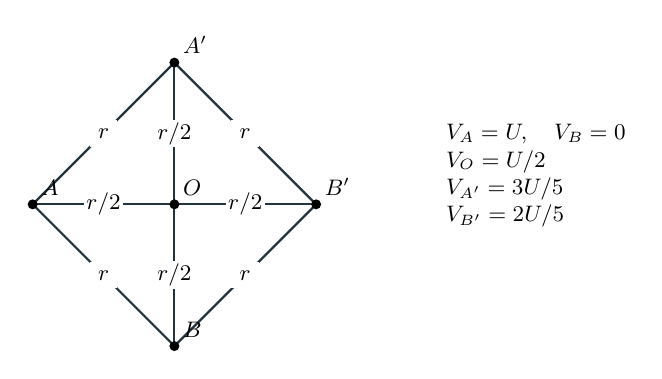
\begin{tikzpicture}[scale=.9,transform shape]

\draw[object](0,0)--(2,2)--(4,0)--(2,-2)--cycle;
\draw[object](0,0)--(4,0) (2,-2)--(2,2);
\foreach \x/\y/\s in {0/0/A,2/2/{A'},4/0/{B'},2/-2/B,2/0/O}{\fill(\x,\y) circle(2pt) node[above right]{$\s$};}
\foreach \x/\y in {1/1,3/1,3/-1,1/-1}{\node[fill=white] at(\x,\y){$r$};}
\foreach \x/\y in {1/0,3/0,2/1,2/-1}{\node[fill=white,inner sep=1pt] at(\x,\y){$r/2$};}
\node[align=left] at(7.1,.4){$V_A=U,\quad V_B=0$\\$V_O=U/2$\\$V_{A'}=3U/5$\\$V_{B'}=2U/5$};

\end{tikzpicture}
\figcaption{解图电4.10A\quad 上下两个对称节点压为$O$，平面图的四条径向支路已各并联成$r/2$。}
\end{minipage}\end{center}

解图电4.10A把相对$A,B$端口上下对称的两个交点合并为$O$，两个并联四分之一圆弧合为$r/2$。其余四点构成圆周$A,A',B',B$，每条外边为$r$；$O$到这四点各为$r/2$。

固定$V_A=U,V_B=0$，交换$A,B$并反号平移电势可知$V_O=U/2$，另外两点的电势也分别满足$V_{A'}+V_{B'}=U$。在$A'$处列式：
\[
\frac{V_{A'}-U}{r}+\frac{V_{A'}-V_{B'}}r+\frac{V_{A'}-U/2}{r/2}=0.
\]
解得$V_{A'}=3U/5,V_{B'}=2U/5$。因此从$A$流出的三类电流为
\[
I_{AA'}=\frac{2U}{5r},\quad I_{AB}=\frac Ur,\quad
I_{AO}=\frac{U/2}{r/2}=\frac Ur.
\]
相加得$I=12U/(5r)$，所以
\[
\boxed{R_{AB}=\frac{5r}{12}=\frac{5R}{48}}.
\]
沿解图电4.10A也可利用$O$处两对对应电流，等效地把交叉连接拆成$A\to O\to B$及$A'\to O\to B'$两条不互接的路径。于是$AB$间直接支路为$r\parallel r=r/2$，另外一条沿$A\to A'\to B'\to B$的路径为$r+(r\parallel r)+r=5r/2$，二者并联仍给$5r/12$。拆点依据下面的电流配对。拆开后两个半点分别满足节点守恒。

\begin{center}\begin{minipage}{.97\linewidth}\centering
\begin{tikzpicture}[scale=.95,font=\small]
\draw[object](0,0)--(2,2)--(4,0)--(2,-2)--cycle;
\draw[object](0,0)--(1.65,-.2)--(2,-2) (2,2)--(2.35,.2)--(4,0);
\foreach \x/\y/\s in {0/0/A,2/2/{A'},4/0/{B'},2/-2/B}{\fill(\x,\y)circle(1.5pt)node[above right]{$\s$};}
\fill(1.65,-.2)circle(1.4pt);\fill(2.35,.2)circle(1.4pt);\draw[guide](1.65,-.2)--(1.4,-.5);\node[below]at(1.4,-.5){$O_1$};\draw[guide](2.35,.2)--(2.6,.5);\node[above]at(2.6,.5){$O_2$};
\foreach \x/\y in {1/1,3/1,3/-1,1/-1}{\node[draw,fill=white]at(\x,\y){$r$};}
\foreach \x/\y in {.8/-.1,1.83/-1.1,2.17/1.1,3.2/.1}{\node[fill=white,inner sep=1pt]at(\x,\y){$r/2$};}
\node[right,align=left]at(5.2,.7){$I_{AO_1}=I_{O_1B}=U/r$\\$I_{A'O_2}=I_{O_2B'}=U/(5r)$\\$V_{O_1}=V_{O_2}=U/2$\\$O_1,O_2$互不连接};
\end{tikzpicture}
\figcaption{解图电4.10B　按已证明相等的两对电流拆开O点。拆后两个节点分别流入等于流出，全部支路电势差保持。}
\end{minipage}\end{center}

解图电4.10B把拆点条件落到实际电流上。A到O的电流为$(U-U/2)/(r/2)=U/r$，O到B也为$U/r$；A'到O为$(3U/5-U/2)/(r/2)=U/(5r)$，O到B'也为$U/(5r)$。
因此可分别接成 $A\to O_1\to B$ 与 $A'\to O_2\to B'$。两个分点均为 $U/2$，各自流入、流出的电流相等。
拆开后既有电势仍解全部节点方程，正电阻网络的解唯一，端口电流因此保持。
\begin{center}\begin{minipage}{.97\linewidth}\centering
\begin{tikzpicture}[scale=.9,font=\small]
\draw[object](0,0)--(0,2)--(6,2)--(6,0)--cycle;
\node[draw,fill=white]at(1,2){$r$};\node[draw,fill=white]at(3,2){$r/2$};\node[draw,fill=white]at(5,2){$r$};\node[draw,fill=white]at(3,0){$r/2$};
\fill(0,0)circle(1.5pt)node[below left]{$A$};\fill(6,0)circle(1.5pt)node[below right]{$B$};
\fill(2,2)circle(1.4pt)node[above]{$A'$};\fill(4,2)circle(1.4pt)node[above]{$B'$};
\node[right,align=left]at(7,1){上路：$5r/2$\\下路：$r/2$\\并联：$5r/12$};
\end{tikzpicture}
\figcaption{解图电4.10C　拆点后两次局部并联，再归为A、B之间两条内部不相连的通路；两支路电压相同，电阻按并联合成。}
\end{minipage}\end{center}

解图电4.10C中，下路的$r/2$由两条r通路并联：水平外弧AB为r，经$O_1$为$r/2+r/2=r$。
上路中间的$r/2$同理由外弧A'B'的r与经$O_2$的r并联得到；两边AA'、B'B没有合并，仍各为r。
因而两条最终通路为$5r/2$和$r/2$。固定端口电压U时，电流分别为$2U/(5r)$和$2U/r$，相加给$12U/(5r)$，与A图节点法完全一致。

回到题图的立体网络，将合并前的两个接点记为S、T，它们是垂直于AB平面的那条直径两端，均与A、A'、B'、B用四段r圆弧相连，且S、T互为对径而没有直接四分之一弧。
对固定的相邻端口A、B，交换S、T保持整个连接及边界电势，因此$V_S=V_T$；再交换源汇并反号平移，得到其共同值$U/2$。
把两点合成O后，O到四个外点的连接各由两条r并联为$r/2$。这里合并的是两个等势真实节点；解图电4.10A中明确标点的 $O$ 是合并后的真实电连接。题图以六个实点标明圆环之间的连接位置。

各环的发热功率由原立体网络各段的电压确定。$AB$ 所在圆环四段电压的大小依次为
\[
 \frac{2U}{5},\qquad \frac U5,\qquad \frac{2U}{5},\qquad U.
\]
各段电阻为 $r$，把四项 $U_i^2/r$ 相加，得该圆环的发热功率 $34U^2/(25r)$。
另外两环各有两段电压$U/2$与两段$U/10$，每环耗散$13U^2/(25r)$；三环总功率为
\[
P=\frac{34+13+13}{25}\frac{U^2}{r}=\frac{12U^2}{5r}=UI.
\]
三个环上的各段电阻相同。AB所在圆环含有横跨端口的整段U压降，故它的发热功率大于另外两环。后两环到S、T的对应两段圆弧具有相同压降，在图B中合成四条$r/2$支路。


\Needspace{13\baselineskip}

\pdfbookmark[2]{第 11 题 无限梯形网络的收敛与有限阶通式}{q11}

\section*{第 11 题\quad 无限梯形网络的收敛与有限阶通式}\label{q:11}

如图电4.11，每一梯形单元由上、下两条串联电阻$R$及右端一条横跨两轨的电阻$R$组成。由$K$个单元组成、最右端不接其他负载的二端网络等效电阻记为$R_K$。证明$\{R_K\}$单调递减且有界；导出递推和显式通式，定量证明收敛，并求无限网络的等效电阻。

\begin{center}\begin{minipage}{.98\linewidth}\centering
\begin{tikzpicture}[scale=.8,transform shape]

\foreach \x in {0,2,4,8}{\draw[object](\x,0)--(\x+2,0) (\x,2)--(\x+2,2);\node[draw,fill=white] at(\x+1,0){$R$};\node[draw,fill=white] at(\x+1,2){$R$};}
\draw[guide](6,0)--(8,0) (6,2)--(8,2);
\foreach \x/\n in {2/1,4/2,6/3,10/K}{\draw[object](\x,0)--(\x,2);\node[draw,fill=white] at(\x,1){$R$};\node[below] at(\x,-.45){$\n$};}
\node[left] at(0,0){$B$};\node[left] at(0,2){$A$};\node at(6,2.7){虚线省去中间单元};\node[right] at(10.3,1){有限截断};

\end{tikzpicture}
\figcaption{图电4.11\quad 每单元含上、下串联电阻及右端跨接电阻，最右没有额外负载。}
\end{minipage}\end{center}

\Needspace{6\baselineskip}\subsection*{解答}

图电4.11中单节的电阻为$R_1=3R$。在最右端增加一节后，原最末横跨电阻$R$多了一条正电阻通路与其并联，其等效值严格减小；这变化逐级传回输入端，故$R_{K+1}<R_K$。全网为正电阻，$R_K>0$，因此在尚未解出通式前已知极限存在。

\begin{center}\begin{minipage}{.98\linewidth}\centering
\begin{tikzpicture}[scale=.9,transform shape]

\draw[object](0,0)--(2,0)--(5,0)--(5,2)--(2,2)--(0,2) (2,0)--(2,2);
\node[draw,fill=white] at(1,0){$R$};\node[draw,fill=white] at(1,2){$R$};\node[draw,fill=white] at(2,1){$R$};\node[draw,fill=white] at(5,1){$R_K$};
\node[left] at(0,0){$B$};\node[left] at(0,2){$A$};\node at(2.5,-.8){$R_{K+1}=2R+(R\parallel R_K)$};
\node[align=left] at(8,1){开路截断：$R_1=3R$\\$R_2=11R/4$\\$R_3=41R/15$};

\end{tikzpicture}
\figcaption{解图电4.11A\quad 剥去左端单元后，右侧整体以$R_K$表示，两个纵轨电阻仍串联。}
\end{minipage}\end{center}

解图电4.11A也可从左端剥去一节：上、下两个$R$串在$R\parallel R_K$之外，故
\[
R_{K+1}=2R+\frac{RR_K}{R+R_K}.
\]
令$x_K=R_K/R$，得到
\[
x_1=3,\qquad x_{K+1}=\frac{3x_K+2}{x_K+1}.
\]
求显式解时，先求这一分式变换的不动点：$x^2-2x-2=0$，记$\alpha=1+\sqrt3,\beta=1-\sqrt3$。直接代数化简给
\[
\frac{x_{K+1}-\alpha}{x_{K+1}-\beta}
=\frac{2-\sqrt3}{2+\sqrt3}\frac{x_K-\alpha}{x_K-\beta}.
\]
因$\lambda=(2-\sqrt3)^2=(2-\sqrt3)/(2+\sqrt3)$，且$(x_1-\alpha)/(x_1-\beta)=\lambda$，可逐次迭代为
\[
\frac{x_K-\alpha}{x_K-\beta}=\lambda^K,
\qquad x_K=\frac{\alpha-\beta\lambda^K}{1-\lambda^K}.
\]
整理得到所求的有限阶通式
\[
\boxed{R_K=R\left[1+\sqrt3+\frac{2\sqrt3}{(2+\sqrt3)^{2K}-1}\right]}.
\]
由于$0<\lambda<1$，末项严格为正并随$K$增大递减，故
\[
(1+\sqrt3)R<R_K\le3R,\qquad
\boxed{R_{AB}=\lim_{K\to\infty}R_K=(1+\sqrt3)R}.
\]
由通式可直接读出截断误差：$R_K-R_{AB}=2\sqrt3R\lambda^K/(1-\lambda^K)$。若只需求极限，在已证明收敛后，也可对递推式取极限，得到同一二次方程并排除负根。极限存在之后，递推式的连续性使极限满足不动点方程，正下界选定正根。

\begin{center}\begin{minipage}{.97\linewidth}\centering
\begin{tikzpicture}[x=8cm,y=7cm,font=\small]
\draw[axis](2.65,2.65)--(3.1,2.65)node[below right]{$x_K$};\draw[axis](2.65,2.65)--(2.65,3.1)node[above]{$x_{K+1}$};
\draw[guide](2.65,2.65)--(3.06,3.06);
\draw[traj,domain=2.65:3.06,samples=90,variable=\t]plot(\t,{(3*\t+2)/(\t+1)});
\draw[force](3,3)--(3,2.75)--(2.75,2.75)--(2.75,2.733333)--(2.733333,2.733333);
\fill(2.732051,2.732051)circle(1.4pt);\node[above right]at(3,3){$x_1=3$};
\node[below]at(3,2.65){$3$};\node[left]at(2.65,3){$3$};
\node[right,align=left]at(3.15,3){$f(x)=(3x+2)/(x+1)$};\node[right]at(3.15,2.85){虚线：$y=x$};\node[right]at(3.15,2.7){交点：$\alpha=1+\sqrt3$};
\end{tikzpicture}
\figcaption{解图电4.11B　开路截断递推的局部图。按竖直到函数曲线、水平到对角线的顺序迭代；点的距离按实际数值绘制，后期迭代很快贴近正不动点。}
\end{minipage}\end{center}

\Needspace{8\baselineskip}
用合并一节的等效电阻函数描述末端变化怎样逐级传到输入端。增加一节时，最末横跨R与新增的$3R$通路并联为$3R/4<R$。
对任意正的后方等效电阻T，向前合一节的函数为$F(T)=2R+RT/(R+T)$，导数$F'(T)=R^2/(R+T)^2>0$。
因此后方等效值的严格减小，会经过每一个前方单元仍保持严格减小；网络含有始终串联在输入端的两个R，还给出$R_K>2R$。这一段不使用未知极限值，先把存在性证明独立完成。
解图电4.11B再以实际数值显示$3\to11/4\to41/15$，它与上式的严格递减一致。

也可从移项后的数列构造等比辅助量。由$x_{K+1}+1/(x_K+1)=3$，令$y_K=x_K+1$，便有
\[
y_1=4,\qquad y_{K+1}+\frac1{y_K}=4.
\]
再取$z_K=(y_K+a_1)/(y_K+a_2)$，其中两个参数尚待选择。将$1/y_K=4-y_{K+1}$代入并把分子分母的系数分别提出：
\[
z_K=\frac{1+a_1(4-y_{K+1})}{1+a_2(4-y_{K+1})}
=\frac{a_1}{a_2}\frac{y_{K+1}-(4+1/a_1)}{y_{K+1}-(4+1/a_2)}.
\]
若令$-(4+1/a_i)=a_i$，即$a_i^2+4a_i+1=0$，便把同一分式变换化为等比关系。
取两个不同根$a_1=-2+\sqrt3,a_2=-2-\sqrt3$，得到
\[
z_{K+1}=\frac{a_2}{a_1}z_K=(2+\sqrt3)^2z_K,\qquad
z_1=\frac{4+a_1}{4+a_2}=(2+\sqrt3)^2.
\]
所以$z_K=(2+\sqrt3)^{2K}$。反解定义时，先移项$(z_K-1)y_K=a_1-z_Ka_2$，再整理为
\[
y_K=\frac{a_1-a_2}{z_K-1}-a_2
=\frac{2\sqrt3}{(2+\sqrt3)^{2K}-1}+2+\sqrt3.
\]
最后减去1并乘R，就给出前面的有限阶通式。初值 $z_1=q^2$ 与每步乘因子 $q^2$ 共同给指数 $2K$，其中 $q=2+\sqrt3$。

若把 $a_1,a_2$ 选成同一个根，$z$ 恒为1，反解 $y$ 时系数 $z-1$ 为零。因此此变换取两个不同的根。
交换两个不同的根后，参数 $z$ 取倒数。将它代入相应的反变换，得到同一个电阻值 $y$。
这里的$z_K$与前面用不动点直接构造的$(x_K-\alpha)/(x_K-\beta)$恰好互为倒数，两个完整推导的初始指数因此一致。
\begin{center}\begin{minipage}{.97\linewidth}\centering
\begin{tikzpicture}[x=.8cm,y=.5cm,font=\small]
\draw[axis](.5,0)--(6.5,0)node[below right]{$K$};\draw[axis](.5,0)--(.5,7.2)node[above]{$-\log_{10}(|R_K-R_\infty|/R)$};
\draw[traj]plot coordinates{(1,0.5719475) (2,1.7459551) (3,2.8919339) (4,4.0359782) (5,5.1798840) (6,6.3237799)};
\draw[thick,warm,dashed]plot coordinates{(1,0.1354588) (2,1.1845276) (3,2.3207466) (4,3.4640853) (5,4.6079404) (6,5.7518326)};
\foreach \x in {1,2,3,4,5,6}{\node[below]at(\x,0){$\x$};}
\foreach \y in {2,4,6}{\node[left]at(.5,\y){$\y$};}
\node[right,accent]at(7,6){开路截断};\node[right,warm]at(7,4){短路截断};\node[right]at(7,2){数值越高，误差越小};
\fill[accent](1,0.5719475)circle(1.2pt);
\fill[accent](2,1.7459551)circle(1.2pt);
\fill[accent](3,2.8919339)circle(1.2pt);
\fill[accent](4,4.0359782)circle(1.2pt);
\fill[accent](5,5.1798840)circle(1.2pt);
\fill[accent](6,6.3237799)circle(1.2pt);
\fill[warm](1,0.1354588)circle(1.2pt);
\fill[warm](2,1.1845276)circle(1.2pt);
\fill[warm](3,2.3207466)circle(1.2pt);
\fill[warm](4,3.4640853)circle(1.2pt);
\fill[warm](5,4.6079404)circle(1.2pt);
\fill[warm](6,5.7518326)circle(1.2pt);
\end{tikzpicture}
\figcaption{解图电4.11C　两种终端截断的真实误差位数。横坐标只取正整数，连接线用于看趋势；两序列从不同侧趋近同一无限网络。}
\end{minipage}\end{center}

解图电4.11C进一步比较开路与短路终端。用同一个$f(x)$迭代，开路可理解为$x_0=\infty$，第一步为3；短路起点为$x_0=0$，第一步为2。
前者从正不动点上方递减，后者从下方递增。记$q=2+\sqrt3$、$\lambda=q^{-2}$，两种误差分别为
\[
\frac{R_K^{(\rm open)}-R_\infty}{R}=\frac{2\sqrt3\lambda^K}{1-\lambda^K},\qquad
\frac{R_\infty-R_K^{(\rm short)}}R=\frac{2\sqrt3q\lambda^K}{1+q\lambda^K}.
\]
两者均趋于零，所以任意被动正负载终止的相同长度网络，其输入电阻夹在短路、开路截断之间，远端边界影响也随K消失。
图的纵坐标为误差的负常用对数。两组误差的首项都正比于 $\lambda^K$，故曲线接近直线，两种有限截断分别从极限的两侧接近。


\Needspace{13\baselineskip}

\pdfbookmark[2]{第 12 题 无限三角柱电阻网的对称折叠}{q12}

\section*{第 12 题\quad 无限三角柱电阻网的对称折叠}\label{q:12}

图电4.12为沿左右两个方向无限延伸的三角柱电阻网。每一截面是三角形，三条边的电阻均为$r$；相邻截面的三个对应顶点用三条纵向电阻$r$相连。$A,B$为同一截面的一对顶点。求两点间的等效电阻，交叉投影只在实点处电连接。

\begin{center}\begin{minipage}{.98\linewidth}\centering
\begin{tikzpicture}[scale=.8,transform shape]

\foreach \k in {-2,-1,0,1,2}{\pgfmathsetmacro{\x}{2*\k}
\draw[object](\x,-1.2)--(\x,1.2)--(\x+.8,0)--cycle;
\fill[accent](\x,-1.2)circle(1.7pt);\fill[accent](\x,1.2)circle(1.7pt);\fill[accent](\x+.8,0)circle(1.7pt);
\ifnum\k<2\draw[object](\x,-1.2)--(\x+2,-1.2) (\x,1.2)--(\x+2,1.2);\draw[guide](\x+.8,0)--(\x+2.8,0);\fi}
\draw[guide](-5,-1.2)--(-4,-1.2) (-5,1.2)--(-4,1.2) (4,-1.2)--(5,-1.2) (4,1.2)--(5,1.2);
\fill(0,-1.2) circle(2pt) node[below]{$A$};\fill(0,1.2) circle(2pt) node[above]{$B$};\node at(0,2.2){所有小段电阻均为$r$};

\end{tikzpicture}
\figcaption{图电4.12\quad 三角形截面沿两侧无限重复，虚线纵轨位于投影后侧。}
\end{minipage}\end{center}

\Needspace{6\baselineskip}\subsection*{解答}

以$A,B$为源和汇，相对于交换这两个顶点并反转电势的对称，所有截面的第三顶点均处在零势。因此第三条纵向轨上的电流为零，可拆去；每一截面剩下的直边$r$与经第三顶点的两边$2r$并联，得到$2r/3$。

\begin{center}\begin{minipage}{.98\linewidth}\centering
\begin{tikzpicture}[scale=.72,transform shape]

\foreach \x in {0,2,4}{\draw[object](\x,0)--(\x,2);\node[draw,fill=white] at(\x,1){$2r/3$};}
\draw[object](0,0)--(4,0) (0,2)--(4,2);\foreach \x in {1,3}{\node[draw,fill=white] at(\x,0){$r$};\node[draw,fill=white] at(\x,2){$r$};}
\node[below] at(2,0){$A$};\node[above] at(2,2){$B$};\node at(2,3){拆第三纵轨后};
\draw[object](6,0)--(11,0)--(11,2)--(6,2)--cycle (8.5,0)--(8.5,2);
\node[draw,text=warm,fill=white] at(6,1){$2r/3$};\node[draw,fill=white] at(8.5,1){$r/3$};\node[draw,fill=white] at(11,1){$X$};
\node[draw,fill=white] at(7.2,0){$r/2$};\node[draw,fill=white] at(7.2,2){$r/2$};
\node at(8.5,3){左右折叠并剥去一节};\node at(8.5,-1){中央跨接$\parallel$半无限尾部};

\end{tikzpicture}
\figcaption{解图电4.12A\quad 第三顶点间纵轨无电流，斜边仍保留为$2r$路径；折叠时中央跨接不除二。}
\end{minipage}\end{center}

解图电4.12A中，网络成为横跨电阻为$2r/3$、两纵轨每段为$r$的双向无限梯形。沿$AB$左右对称折叠后，两侧对应轨段并联为$r/2$，其余各截面的对应横跨并联为$r/3$。中央横跨在折叠轴上只出现一次，阻值为 $2r/3$。

记不含$AB$直跨支路的折叠半无限尾部电阻为$X$。剥离一节，上、下各$r/2$与$r/3\parallel X$串联，故
\[
X=r+\frac{(r/3)X}{r/3+X}
=\frac{4rX+r^2}{3X+r}.
\]
化为$3X^2-3rX-r^2=0$，取正根
\[
X=\frac{3+\sqrt{21}}6r.
\]
于是输入端还需把本身的$2r/3$并回：
\[
\boxed{R_{AB}=\left(\frac{3}{2r}+\frac1X\right)^{-1}
=\frac{2\sqrt{21}}{21}r=\frac{2r}{\sqrt{21}}}.
\]
这里采用有限开路尾部的极限。若$X_1=4r/3$，递推$X_{k+1}=r+(r/3)\parallel X_k$保持$X_k\ge r$；其导数为$r^2/(3X+r)^2\le1/16$，故尾部迭代收敛且正不动点唯一。所以有限开路尾部从初值迭代收敛，极限正是所求的正不动点。

也可在解图电4.12A直接保留左右两侧计算。记单侧尾部为$Y$，则$Y=2r+(2r/3)\parallel Y$，解得$Y=2X$。中央输入为$(2r/3)\parallel Y\parallel Y$，同样等于$(2r/3)\parallel X$，可复核折叠时的二倍因子。

\begin{center}\begin{minipage}{.97\linewidth}\centering
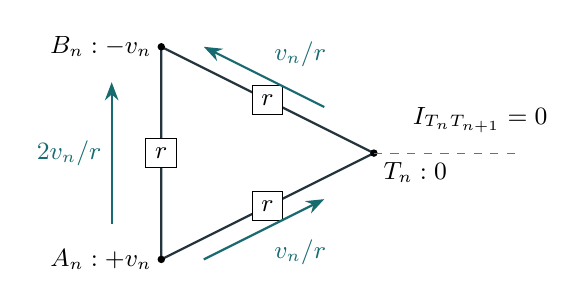
\begin{tikzpicture}[scale=.9,font=\small]
\draw[object](0,-1.5)--(0,1.5)--(3,0)--cycle;
\node[draw,fill=white]at(0,0){$r$};\node[draw,fill=white]at(1.5,.75){$r$};\node[draw,fill=white]at(1.5,-.75){$r$};
\fill(0,-1.5)circle(1.5pt)node[left]{$A_n:+v_n$};\fill(0,1.5)circle(1.5pt)node[left]{$B_n:-v_n$};
\fill(3,0)circle(1.5pt)node[below right]{$T_n:0$};
\draw[motion](-.7,-1)--(-.7,1)node[midway,left]{$2v_n/r$};
\draw[motion](.6,-1.5)--(2.3,-.65)node[midway,below right]{$v_n/r$};
\draw[motion](2.3,.65)--(.6,1.5)node[midway,above right]{$v_n/r$};
\draw[guide](3,0)--(5,0);\node[above]at(4.5,.15){$I_{T_nT_{n+1}}=0$};
\end{tikzpicture}
\figcaption{解图电4.12B　单个截面的电流与第三轨。经$T_n$的两斜边仍各有电流，只有连接各零势$T_n$的纵轨无电流。}
\end{minipage}\end{center}

解图电4.12B逐截面检查拆轨的范围。采用源汇反号的电势基准，令第n个截面A、B对应顶点为$+v_n,-v_n$，第三顶点为零。
直接r边中电流为$2v_n/r$；两条斜边各为$v_n/r$，一条流入第三顶点，另一条流出，故这一点仍传递电流。相邻第三顶点之间的电势差却严格为零，纵轨才能删去。
三角柱投影中各真实顶点已用点标出，后轨与竖边的投影交叉处没有接点，真实电连接在标出的各截面顶点。
\begin{center}\begin{minipage}{.97\linewidth}\centering
\begin{tikzpicture}[scale=.9,font=\small]
\draw[object](0,0)--(0,2)--(5,2)--(5,0)--cycle (3,0)--(3,2);
\node[draw,fill=white,text=warm]at(0,1){$2r/3$};\node[draw,fill=white]at(1.5,0){$r/2$};\node[draw,fill=white]at(1.5,2){$r/2$};
\node[draw,fill=white]at(3,1){$r/3$};\node[draw,fill=white]at(5,1){$X_{N-1}$};
\draw[guide](.7,-.4)rectangle(5.7,2.4);\node[above]at(3.1,2.5){框内尾部：$X_N$};
\fill(0,0)circle(1.5pt)node[below left]{$A$};\fill(0,2)circle(1.5pt)node[above left]{$B$};
\node[right,align=left]at(6.2,1){中央支路不在$X_N$内\\$X_1=4r/3$\\$X_{N}=r+(r/3)\parallel X_{N-1}$};
\end{tikzpicture}
\figcaption{解图电4.12C　有限尾部的递推定义（$N\ge2$）。虚线框包括第一对轨段与后方全部尾部，中央$2r/3$只在最终输入并联一次。}
\end{minipage}\end{center}

解图电4.12C将有限尾部与中央支路分开。最少一节的框内只包括两条$r/2$和末端$r/3$，所以$X_1=4r/3$。
增加一节后，框内第一对轨段仍与$r/3\parallel X_{N-1}$串联，得到既有递推；框外中央$2r/3$独立保留，输入为$(2r/3)\parallel X_N$。
$X_N$ 从框内的第一对纵轨开始，包含这对轨段与右端横跨和后续尾部的并联项。

用未折叠的梯形网直接求各截面的电势。对$n\ne0$处A侧节点列守恒，两个邻截面的纵向电流与横向电流相加为零：
\[
\frac{v_n-v_{n-1}}r+\frac{v_n-v_{n+1}}r+\frac{2v_n}{2r/3}=0,
\qquad v_{n+1}-5v_n+v_{n-1}=0.
\]
特征根为$(5\pm\sqrt{21})/2$，被动开路截断的有界极限应舍去向远处增长的一根。记$\eta=(5-\sqrt{21})/2$，左右对称及$v_0=V$给
\[
v_n=V\eta^{|n|},\qquad 0<\eta<1.
\]
在输入截面，横向$r\parallel2r$贡献$3V/r$，左右两条A侧纵轨各贡献$V(1-\eta)/r$，所以
\[
I=\frac{V}{r}[3+2(1-\eta)]=\frac{\sqrt{21}V}{r},\qquad
R_{AB}=\frac{2V}{I}=\frac{2r}{\sqrt{21}}.
\]
端口电压为 $2V$。空间因子 $\eta$ 表示每向外一步的电势比；增加一节截断网络造成的等效电阻误差，由尾部函数的导数控制。


\Needspace{13\baselineskip}

\pdfbookmark[2]{第 13 题 七电阻单元串接成的无限网络}{q13}

\section*{第 13 题\quad 七电阻单元串接成的无限网络}\label{q:13}

图电4.13所示单元由七只阻值均为$r$的电阻组成。输入端$P$在左上角，输入端$Q$用理想导线与右下角相连；输出端$p,q$分别在右上、右下角。把每一单元的$p,q$与下一单元的$P,Q$相接，无限延伸，求输入电阻。

\begin{center}\begin{minipage}{.98\linewidth}\centering
\begin{tikzpicture}[scale=.72,transform shape]

\foreach \x in {0,1.8,3.6}{\draw (\x,0)--(\x,2);}
\draw (0,0)--(3.6,0) (0,2)--(3.6,2);
\draw (-.6,-.9)--(3.6,-.9)--(3.6,0);
\draw (-.6,2)--(0,2) (3.6,2)--(4.3,2) (3.6,0)--(4.3,0);
\node[left] at(-.6,2){$P$};\node[left] at(-.6,-.9){$Q$};
\node[right] at(4.3,2){$p$};\node[right] at(4.3,0){$q$};
\foreach \x in {0,1.8,3.6}{\fill(\x,0)circle(1.5pt);\fill(\x,2)circle(1.5pt);}
\node at(1.8,2.7){七条边各为$r$};
\foreach \x in {0,1.8,3.6}{\node[draw,fill=white]at(\x,1){$r$};}\foreach \x in {.9,2.7}{\node[draw,fill=white]at(\x,0){$r$};\node[draw,fill=white]at(\x,2){$r$};}
\draw[->] (5,1)--(6,1);
\foreach \x in {6.5,8,9.5}{\draw(\x,0)rectangle++(1,2);}
\node at(7,1){单元};\node at(8.5,1){单元};\node at(10,1){$\cdots$};
\draw(7.5,.4)--(8,.4) (7.5,1.6)--(8,1.6) (9,.4)--(9.5,.4) (9,1.6)--(9.5,1.6);

\end{tikzpicture}
\figcaption{图电4.13\quad 单元下端的绕接导线与逐级连接}
\end{minipage}\end{center}

\Needspace{6\baselineskip}\subsection*{解答}

先截取有限个单元，末端开路，输入电阻记为$R_K$。在前方加一个单元时，它右侧竖直电阻$r$与后方的$R_K$并联。解图电4.13A把串联的无分支节点消去，右上支路成为
\[
R_x=r+(r\parallel R_K)=\frac{r(r+2R_K)}{r+R_K}.
\]
左下两只电阻串联为$2r$，中间竖直电阻连接两个内节点，保留其支路电流。

\begin{center}\begin{minipage}{.98\linewidth}\centering
\begin{tikzpicture}[scale=.85,transform shape]

\coordinate(A)at(0,1.4);\coordinate(U)at(2,3);\coordinate(V)at(2,0);\coordinate(B)at(4,1.4);
\draw(A)--node[above left]{$r,\ I_1$}(U)--node[above right]{$R_x,\ I_2$}(B)
(A)--node[below left]{$2r,\ I-I_1$}(V)--node[below right]{$r,\ I-I_2$}(B)
(U)--node[right]{$r,\ I_1-I_2$}(V);
\foreach \p in{A,U,V,B}{\fill(\p)circle(1.5pt);\node[above]at(\p){$\p$};}
\draw[->,blue](-1,1.4)--(-.1,1.4)node[midway,above]{$I$};
\node[align=left]at(7,1.4){$R_x=r+(r\parallel R_K)$\\$Q$与$B$为同一节点};

\end{tikzpicture}
\figcaption{解图电4.13A\quad 先保留桥臂，再替换尾网}
\end{minipage}\end{center}

设总电流$I$由$A$流向$B$，$A\to U$电流为$I_1$，$U\to B$为$I_2$。则$U\to V$为$I_1-I_2$，$A\to V$为$I-I_1$，$V\to B$为$I-I_2$。分别比较两条$A\to V$路径和两条$U\to B$路径：
\[
I_1r+(I_1-I_2)r=2r(I-I_1),\qquad
I_2R_x=r(I_1-I_2)+r(I-I_2).
\]
解得
\[
I_1=\frac{2R_x+5r}{4R_x+7r}I,\quad
I_2=\frac{6r}{4R_x+7r}I.
\]
沿解图电4.13A的$A,U,B$计算电压，得到递推式
\[
R_{K+1}=\frac{I_1r+I_2R_x}{I}
=r\frac{8R_x+5r}{4R_x+7r}
=r\frac{13r+21R_K}{11r+15R_K}.
\]
开路终端给$R_1=7r/5$。令$x_K=R_K/r$，映射$f(x)=(13+21x)/(11+15x)$把正半轴映入$(13/11,7/5)$，且
\[
0<f'(x)=\frac{36}{(11+15x)^2}\le\frac{36}{121}<1.
\]
因此有限截断有唯一正极限，可令$R_{K+1}=R_K=R_\infty$。解
$15(R_\infty/r)^2-10(R_\infty/r)-13=0$，舍去负根，得
\[
\boxed{R_\infty=\frac{5+2\sqrt{55}}{15}\,r}.
\]
题图中的 $Q$ 沿理想导线与右下角同节点，所以左下两只电阻之间的连接点无其他支路。

\begin{center}\begin{minipage}{.97\linewidth}\centering
\begin{tikzpicture}[scale=.95,font=\small]
\draw[object](0,0)--(1.8,0)--(1.8,1)--(4,1)--(4,-1)--(1.8,-1)--(1.8,0) (4,0)--(5,0);
\node[draw,fill=white]at(.9,0){$r$};\node[draw,fill=white]at(2.9,1){$r$};\node[draw,fill=white]at(2.9,-1){$R_K$};
\fill(0,0)circle(1.4pt)node[left]{$U$};\fill(5,0)circle(1.4pt)node[right]{$B$};
\node[right,align=left]at(6,0){先串联一个$r$\\后接$r\parallel R_K$\\整体记为$R_x$};
\end{tikzpicture}
\figcaption{解图电4.13B　五臂桥中U、B之间支路的内部连接。尾网与右侧竖直r并联，再与上轨r串联；绕接导线使Q与B同属一个节点。}
\end{minipage}\end{center}

解图电4.13B将$R_x$内部两步拆开，也明确初值的含义。末端开路时，$r\parallel\infty=r$，单元右侧的竖直 $r$ 仍保留，故单个单元的 $R_x=r+r=2r$。
输入Q经理想导线直接到B，左侧竖直r与左下水平r之间没有分支，才能组成$2r$。若把Q接在左下角，两电阻不再处于这一串联关系，整个五臂桥模型已被改变。

将两条回路式整理为
\[
4I_1-I_2=2I,\qquad -rI_1+(R_x+2r)I_2=rI.
\]
由第一式$I_2=4I_1-2I$，代入第二式得$(4R_x+7r)I_1=(2R_x+5r)I$；再代回第一式得到$I_2=6rI/(4R_x+7r)$。
沿A、U、B的压降为$I_1r+I_2R_x$，化为$r(8R_x+5r)/(4R_x+7r)$。将B图的$R_x$代入时，同乘$r+R_K$分别整理分子、分母，得到$13r+21R_K$与$11r+15R_K$，最后保留外乘的r才有正确电阻量纲。
\begin{center}\begin{minipage}{.97\linewidth}\centering
\begin{tikzpicture}[scale=.8,font=\small]
\draw[object](0,-2)--(0,2)--(6,2)--(6,-2)--cycle (3,-2)--(3,2);
\node[draw,fill=white]at(1.5,2){$r$};\node[draw,fill=white]at(4.5,2){$R_x$};\node[draw,fill=white]at(1.5,-2){$2r$};\node[draw,fill=white]at(4.5,-2){$r$};\node[draw,fill=white]at(3,0){$r$};
\draw[motion](.5,2.5)--(2.5,2.5)node[midway,above]{$0.613I_0$};\draw[motion](3.5,2.5)--(5.5,2.5)node[midway,above]{$0.452I_0$};
\draw[motion](.5,-2.5)--(2.5,-2.5)node[midway,below]{$0.387I_0$};\draw[motion](3.5,-2.5)--(5.5,-2.5)node[midway,below]{$0.548I_0$};
\draw[motion](3.6,1)--(3.6,-1)node[midway,right]{$0.161I_0$};
\fill(0,0)circle(1.5pt)node[left]{$A$};\fill(6,0)circle(1.5pt)node[right]{$B$};\fill(3,2)circle(1.5pt)node[above]{$U$};\fill(3,-2)circle(1.5pt)node[below]{$V$};
\draw[motion](-1.3,0)--(-.1,0)node[midway,above]{$I_0$};\draw[motion](6.1,0)--(7.3,0)node[midway,above]{$I_0$};
\end{tikzpicture}
\figcaption{解图电4.13C　无限极限时五臂桥的实际电流比例，图中数值取三位小数。中桥电流沿图的竖直支路向下。}
\end{minipage}\end{center}

解图电4.13C采用$x_\infty=(5+2\sqrt{55})/15\simeq1.3221598$，对应$R_x/r\simeq1.5693664$，所以$I_1/I\simeq0.6129734$、$I_2/I\simeq0.4518935$。
中桥电流为$I_1-I_2\simeq0.1610799I$，两下方支路分别为$0.3870266I$与$0.5481065I$。在两处连接点，流入的电流恰等于沿相邻支路流出的电流。
对任意非负被动尾阻都有$r\le R_x\le2r$，于是
\[
\frac{I_1-I_2}{I}=\frac{2R_x-r}{4R_x+7r}>0.
\]
所以任何非负尾部负载下，中桥电流都由 $U$ 流向 $V$。

收敛证明可进一步把范围说清。一次迭代后所有非负尾阻进入$[13/11,7/5]$，连续映射f保持该闭区间不变，且导数绝对值始终小于1，因此它是完整闭区间上的压缩映射。
负的代数固定点不在这一被动区间内。任取非负的有限尾阻或开路，迭代进入同一不变区间，从各初值都收敛到这个正不动点。

在无限网络中计算每一单元送入后方尾网的电流。B图并联处分入真正后方尾网的电流记为J，则
\[
\frac JI=\frac{I_2}{I}\frac{r}{r+R_\infty}
=\frac6{11+15x_\infty}=\frac3{8+\sqrt{55}}\simeq0.1946005.
\]
相同单元逐级重复，越过K个单元的尾部输入电流为$I(J/I)^K$，因此远端电流和剩余耗散都迅速减小，但有限位置的尾部并非严格开路。
这个比例的平方恰等于$f'(x_\infty)$，将等效电阻的迭代灵敏度与实际网络中的电流传递联系起来。


\Needspace{13\baselineskip}

\pdfbookmark[2]{第 14 题 逐级折半的三角形导线网}{q14}

\section*{第 14 题\quad 逐级折半的三角形导线网}\label{q:14}

用单位长度电阻为$r$的均匀导线组成边长$a$的正三角形，并依次连接每一级三角形三边的中点，得到无限嵌套网络，如图电4.14。各交点均电连接。求外三角形一条边的两个端点$A,B$之间的电阻。

\begin{center}\begin{minipage}{.98\linewidth}\centering
\begin{tikzpicture}[scale=.75,transform shape]
\draw (0.00000,0.00000)--(6.00000,0.00000)--(3.00000,5.19615)--cycle;
\draw (3.00000,0.00000)--(4.50000,2.59808)--(1.50000,2.59808)--cycle;
\draw (3.75000,1.29904)--(3.00000,2.59808)--(2.25000,1.29904)--cycle;
\draw (3.37500,1.94856)--(2.62500,1.94856)--(3.00000,1.29904)--cycle;
\draw (3.00000,1.94856)--(2.81250,1.62380)--(3.18750,1.62380)--cycle;
\node[below left]at(0,0){$A$};\node[below right]at(6,0){$B$};
\node[below]at(3,0){$O$};\node[left]at(1.5,2.598){$P$};\node[right]at(4.5,2.598){$Q$};
\node at(5,4){$\cdots$};\draw[<->](0,-.8)--node[fill=white]{$a$}(6,-.8);

\end{tikzpicture}
\figcaption{图电4.14\quad 中点三角形继续无限嵌套}
\end{minipage}\end{center}

\Needspace{6\baselineskip}\subsection*{解答}

设所求为$R$，外边$AB$的中点为$O$，另两边中点为$P,Q$。网络关于$AB$的中垂线对称。取$A,B$电势为$\pm U/2$，反射并反号后解不变，所以对称轴上的节点均为零电势。

在 $O$ 处沿外边和内网分别写电流守恒。沿$AO,OB$的两电流相等，进入与离开内网$O$的两侧电流也因反射相等，各自满足节点守恒。因此可把$O$处分成两个同电势而互不相连的节点，分别属于外边与内部网络。

\begin{center}\begin{minipage}{.98\linewidth}\centering
\begin{tikzpicture}[scale=.85,transform shape]

\draw(0,0)--(7,0) (0,0)--(0,2)--(1.5,2);
\draw(1.5,2)--(1.5,3.2)--(5.5,3.2)--(5.5,2)--(7,2)--(7,0);
\draw(1.5,2)--(1.5,1.1)--(5.5,1.1)--(5.5,2);
\node[below]at(0,0){$A$};\node[below]at(7,0){$B$};
\fill(1.5,2)circle(1.5pt);\fill(5.5,2)circle(1.5pt);
\node[above left]at(1.5,2.25){$P$};\node[above right]at(5.5,2.25){$Q$};
\node[fill=white]at(.7,2){$ar/2$};\node[fill=white]at(6.3,2){$ar/2$};
\node[fill=white]at(3.5,3.2){$ar$};\node[fill=white]at(3.5,1.1){$X=R/2$};
\node[fill=white]at(3.5,0){$ar$};
\node at(3.5,4){将$O$处分为各自平衡的两个节点};

\end{tikzpicture}
\figcaption{解图电4.14A\quad 分裂轴上节点后的两条端口路径}
\end{minipage}\end{center}

解图电4.14A中，$P,Q$之间沿外顶点的路径电阻为$ar$；内部网络与整个网络相似、线性尺寸为一半，故内部端口电阻为$X=R/2$。外侧$AP,QB$各为$ar/2$。于是
\[
R=ar\parallel\left[ar+(ar\parallel X)\right]
=ar\,\frac{ar+2X}{2ar+3X},\qquad X=\frac R2.
\]
令$x=R/(ar)$，得$3x^2+2x-2=0$。正根为
\[
\boxed{R=\frac{\sqrt7-1}{3}\,ar}.
\]
此处$r$的单位为$\Omega/\mathrm m$，$ar$才是电阻。逐级增加内部导线只会降低端口电阻；同时端点$A$引出的两段长度均为$a/2$，将后方全部短接后仍有下界$ar/4$。因此有限截断电阻单调有界，极限存在，使用自相似关系有依据。

\begin{center}\begin{minipage}{.97\linewidth}\centering
\begin{tikzpicture}[scale=.82,font=\small]
\draw[object](0,0)--(3,0) (0,2)--(1.5,0)--(3,2);
\fill(1.5,0)circle(1.5pt);\draw[guide](1.5,-.08)--(1.5,-1.05);\node at(1.5,-1.25){$O:0$};
\node[left]at(0,0){$A$};\node[right]at(3,0){$B$};\node[above]at(0,2){$P_1$};\node[above]at(3,2){$Q_1$};
\draw[motion](.2,-.45)--(1.1,-.45)node[midway,below]{$J$};\draw[motion](1.9,-.45)--(2.8,-.45)node[midway,below]{$J$};
\draw[motion](.1,1.45)--(.7,.65)node[midway,left]{$K$};\draw[motion](2.3,.65)--(2.9,1.45)node[midway,right]{$K$};
\draw[->,thick](3.7,.6)--(4.7,.6);
\draw[object](5.5,-.4)--(8.5,-.4) (5.5,2)--(7,1)--(8.5,2);
\fill(7,-.4)circle(1.5pt);\draw[guide](7,-.48)--(7,-1.4);\node at(7,-1.65){$O_{\text{外}}:0$};\fill(7,1)circle(1.5pt)node[below]{$O_{\text{内}}:0$};
\node[left]at(5.5,-.4){$A$};\node[right]at(8.5,-.4){$B$};\node[above]at(5.5,2){$P_1$};\node[above]at(8.5,2){$Q_1$};
\draw[motion](5.7,-.85)--(6.6,-.85)node[midway,below]{$J$};\draw[motion](7.4,-.85)--(8.3,-.85)node[midway,below]{$J$};
\draw[motion](5.7,1.55)--(6.3,1.15)node[midway,below left]{$K$};\draw[motion](7.7,1.15)--(8.3,1.55)node[midway,below right]{$K$};
\end{tikzpicture}
\figcaption{解图电4.14B　O附近的局部电流与节点分裂。$P_1,Q_1$是OP、OQ的中点；两对支路各自流入等于流出，分裂后两零势点之间无需导线。}
\end{minipage}\end{center}

解图电4.14B只放大O附近的四条支路。外边两段长度均为$a/2$，两端电势相反，故从A流入与流向B的电流同为$J=U/(ar)$。
内侧相邻节点$P_1,Q_1$也是关于轴的反射点，电势互反；$OP_1,OQ_1$等长，各为$a/4$，故经过O的内侧两股电流也同为K。两对各自满足守恒，拆开后保留原电势分布就仍然满足所有节点方程，唯一性保证端口电流不变。
外边和内网各自的一入一出相等，使拆开的两个节点分别满足守恒。

把半尺度相似关系写成有限层递推。记$R_0=ar$，以$\mathcal R_N$表示外三角形内另有N层中点三角形的端口电阻，$x_N=\mathcal R_N/R_0$。N=0只含外三角形，因此$x_0=2/3$。
加一层后，P、Q内侧是上一级网络的半尺度复制，阻值为$\mathcal R_N/2$。解图电4.14A的串并联式便给
\[
x_{N+1}=G(x_N)=\frac{2(1+x_N)}{4+3x_N},\qquad x_0=\frac23.
\]
\begin{center}\begin{minipage}{.97\linewidth}\centering
\begin{tikzpicture}[x=1.15cm,y=19cm,font=\small]
\draw[->](0,.53)--(4.7,.53)node[right]{$N$};\draw[->](0,.53)--(0,.70)node[above]{$R_N/(ar)$};
\foreach \x in {0,1,2,3,4}{\draw(\x,.53)--(\x,.527)node[below]{$\x$};}
\draw[guide](0,.5485837704)--(4.5,.5485837704);\node[right]at(4.5,.5485837704){$(\sqrt7-1)/3$};
\draw[accent,thick]plot coordinates{(0,0.6666666667) (1,0.5555555556) (2,0.5490196078) (3,0.5486111111) (4,0.5485854859)};
\fill[accent](0,0.6666666667)circle(1.4pt);
\fill[accent](1,0.5555555556)circle(1.4pt);
\fill[accent](2,0.5490196078)circle(1.4pt);
\fill[accent](3,0.5486111111)circle(1.4pt);
\fill[accent](4,0.5485854859)circle(1.4pt);
\node[right,align=left]at(5,.64){$x_0=2/3$\\$x_1=5/9$\\$x_2=28/51$\\$x_3=79/144$\\$x_4=446/813$};
\end{tikzpicture}
\figcaption{解图电4.14C　保留N层中点三角形时的实际有限阻值。各点使用同一纵轴比例；后几个点已很接近水平极限线。}
\end{minipage}\end{center}

解图电4.14C从 $N=0$ 画出有限层端口电阻。$G(1/2)=6/11>1/2$、$G(2/3)=5/9<2/3$，且
\[
\frac{\dd G}{\dd x}=\frac2{(4+3x)^2}>0,\qquad
0<\frac{\dd G}{\dd x}\le\frac8{121}\quad(1/2\le x\le2/3).
\]
因此$[1/2,2/3]$是不变闭区间，压缩映射给唯一固定点；从$x_1<x_0$及G递增，逐次得到$x_{N+1}<x_N$，说明这一正固定点正是开路有限截断的极限。
保留前面的$ar/4$也已足以证明正下界；还可以在不短接A、B的前提下，把其余全部节点短成一个公共节点。A的两段$ar/2$并联为$ar/4$，B端也为$ar/4$，两端串联得到更强的下界
\[
\frac{ar}{2}\le\mathcal R_N\le\frac{2ar}{3}.
\]
两端各自有两段导线接到同一公共节点，A、B之间仍经过两组接入电阻。

沿解图电4.14A计算每一级送入内网的电流。总输入$I=U/R$，外边直接支路流$U/R_0$，另一支路电流为$J_b=I-U/R_0$。
由$P,Q$之间$R_0$与$R/2$并联，真正流入内部网络的电流$J_{\text{内}}=J_bR_0/(R_0+R/2)$。代$\alpha=R/R_0$及$3\alpha^2+2\alpha-2=0$，整理为
\[
\frac{J_{\text{内}}}{I}=\frac{\alpha}{1+\alpha},\qquad
\frac{U_{PQ}}U=\frac{\alpha}{2(1+\alpha)}.
\]
电流比例和电压比例相差二倍，正是内网输入电阻缩为一半。内部网络消耗的功率占总功率的比例为
\[
\lambda=\frac{\alpha^2}{2(1+\alpha)^2}=\frac{2}{(4+3\alpha)^2}=G'(\alpha).
\]
每深入一层，剩余耗散再乘这个小于1的比例。因此无限嵌套仍有有限输入功率，且越向内部，电势差与电流均按各自固定比例减小。
全部导线总长度为$3a\sum_{n=0}^{\infty}2^{-n}=6a$；总长度有限与端口电阻非零可以同时成立，具体端口阻值仍须由连通关系和尺度递推求出。


\Needspace{13\baselineskip}

\pdfbookmark[2]{第 15 题 三个方格的对角端口电阻}{q15}

\section*{第 15 题\quad 三个方格的对角端口电阻}\label{q:15}

用十只相同电阻$R$连接成三个并排的正方形，如图电4.15。求左下端点$A$与右上端点$B$之间的等效电阻。

\begin{center}\begin{minipage}{.98\linewidth}\centering
\begin{tikzpicture}[scale=.9,transform shape]
\draw (0.0,0)--(0.0,2);
\draw (0.0,0)--(1.6,0) (0.0,2)--(1.6,2);
\fill (0.0,0) circle(1.4pt);
\fill (0.0,2) circle(1.4pt);
\draw (1.6,0)--(1.6,2);
\draw (1.6,0)--(3.2,0) (1.6,2)--(3.2,2);
\fill (1.6,0) circle(1.4pt);
\fill (1.6,2) circle(1.4pt);
\draw (3.2,0)--(3.2,2);
\draw (3.2,0)--(4.800000000000001,0) (3.2,2)--(4.800000000000001,2);
\fill (3.2,0) circle(1.4pt);
\fill (3.2,2) circle(1.4pt);
\draw (4.800000000000001,0)--(4.800000000000001,2);
\fill (4.800000000000001,0) circle(1.4pt);
\fill (4.800000000000001,2) circle(1.4pt);
\node[below left] at(0,0){$A$};
\node[above right] at(4.800000000000001,2){$B$};
\node at(2.4000000000000004,-1){每一小边均为$R$};
\end{tikzpicture}
\figcaption{图电4.15\quad 三格网络的对角端口}
\end{minipage}\end{center}

\Needspace{6\baselineskip}\subsection*{解答}

令总电流$I$从$A$进入、从$B$流出。绕图形中心转动$180^\circ$并反转电流，网络和激励均恢复，所以最左、最右竖边的向上电流相等，记为$I_1$。上下中间水平电阻的电流经同一变换互换，而任一竖截面的两条水平电流之和为$I$，故中间两条各为$I_2=I/2$。

\begin{center}\begin{minipage}{.98\linewidth}\centering
\begin{tikzpicture}[scale=.9,transform shape]
\draw (0.0,0)--(0.0,2);
\draw (0.0,0)--(1.6,0) (0.0,2)--(1.6,2);
\fill (0.0,0) circle(1.4pt);
\fill (0.0,2) circle(1.4pt);
\draw[->,blue] (0.13,.55)--(0.13,1.35) node[midway,right]{$i_0$};
\draw (1.6,0)--(1.6,2);
\draw (1.6,0)--(3.2,0) (1.6,2)--(3.2,2);
\fill (1.6,0) circle(1.4pt);
\fill (1.6,2) circle(1.4pt);
\draw[->,blue] (1.73,.55)--(1.73,1.35) node[midway,right]{$i_1$};
\draw (3.2,0)--(3.2,2);
\draw (3.2,0)--(4.800000000000001,0) (3.2,2)--(4.800000000000001,2);
\fill (3.2,0) circle(1.4pt);
\fill (3.2,2) circle(1.4pt);
\draw[->,blue] (3.33,.55)--(3.33,1.35) node[midway,right]{$i_2$};
\draw (4.800000000000001,0)--(4.800000000000001,2);
\fill (4.800000000000001,0) circle(1.4pt);
\fill (4.800000000000001,2) circle(1.4pt);
\draw[->,blue] (4.930000000000001,.55)--(4.930000000000001,1.35) node[midway,right]{$i_3$};
\node[below left] at(0,0){$A$};
\node[above right] at(4.800000000000001,2){$B$};
\node at(2.4000000000000004,-1){每一小边均为$R$};
\node[above]at(1.6,2){$C$};
\foreach \x/\v in{.8/{3I/8},2.4/{I/2},4/{5I/8}}{\draw[->,blue](\x-.4,2.15)--(\x+.4,2.15)node[midway,above]{$\v$};}
\node at(2.4,3.25){$i_0=i_3=3I/8,\quad i_1=i_2=I/8$};

\end{tikzpicture}
\figcaption{解图电4.15A\quad 水平分流与竖边向上电流}
\end{minipage}\end{center}

解图电4.15A将上边从左至右的三个电流标为$I_1,I/2,I-I_1$。由两个内节点的守恒，中间两条竖边向上电流均为$I/2-I_1$。令$C$为上排从左数第二个节点，比较$A\to C$的两条路径：
\[
2I_1R=(I-I_1)R+(I/2-I_1)R.
\]
因此$I_1=3I/8$，两条中间竖边电流各为$I/8$。沿$A$向上、再沿整个上边到$B$求电压：
\[
U_{AB}=I_1R+I_1R+\frac I2R+(I-I_1)R
=\frac{15}{8}IR.
\]
由端口电压与总流之比，
\[
\boxed{R_{AB}=\frac{15}{8}R}.
\]
中心旋转只将左右两端的竖边相互配对，也将两条中间竖边相互配对。两端竖边是$3I/8$，中间竖边是$I/8$，解图上的四个箭头分别对应这些数值。

\begin{center}\begin{minipage}{.97\linewidth}\centering
\begin{tikzpicture}[scale=.9,font=\small]
\draw[object](0,0)--(6,0) (0,2)--(6,2);
\foreach \x in {0,2,4,6}{\draw[object](\x,0)--(\x,2);\fill(\x,0)circle(1.5pt);\fill(\x,2)circle(1.5pt);}
\foreach \x/\v in {0/15,2/10,4/6,6/3}{\node[below]at(\x,-.12){$\v/8$};}
\foreach \x/\v in {0/12,2/9,4/5,6/0}{\node[above]at(\x,2.12){$\v/8$};}
\node[left]at(0,0){$A$};\node[right]at(6,2){$B$};\node[below]at(3,-.85){节点电势单位为$IR$，取$V_B=0$};
\end{tikzpicture}
\figcaption{解图电4.15B　八个节点的实际电势。相邻两点电势差除以R，给出A图中每一条支路的电流与方向。}
\end{minipage}\end{center}

解图电4.15B可从接地的B逐边反推。最右竖边向上$3I/8$，故右下电势$3IR/8$；上排最后一边向右$5I/8$，故右起第二个上节点为$5IR/8$。
继续沿上轨向左，依次加$IR/2$和$3IR/8$，得到$9IR/8$、$12IR/8$。最左竖边再向上降$3IR/8$，输入A为$15IR/8$。
下排自左至右的三股向右电流于是为$5I/8,I/2,3I/8$；两内竖边的下上电势差都为$IR/8$，与A图箭头逐个相符。

可把局部回路的消元再写一步：$2I_1=I-I_1+I/2-I_1=3I/2-2I_1$，故$4I_1=3I/2$，才得到$3I/8$。
从A沿下轨到右下，再向上到B，另一路径给
\[
U_{AB}=\left(\frac58+\frac12+\frac38+\frac38\right)IR=\frac{15}{8}IR.
\]
两条路径由同一个A、B端口约束，压降之和相同。两端与中间竖边分别有非零的向上电流。
\begin{center}\begin{minipage}{.97\linewidth}\centering
\begin{tikzpicture}[x=1.55cm,y=3.2cm,font=\small]
\draw[->](-.6,0)--(4.4,0);\draw[->](-.6,0)--(-.6,.95)node[above]{$P/(RI^2)$};
\foreach \x/\h/\v in {0/.5625/{36/64},1/.03125/{2/64},2/.5/{32/64},3/.78125/{50/64}}{
\filldraw[fill=accent!15,draw=accent](\x-.25,0)rectangle(\x+.25,\h);\node[above]at(\x,\h){$\v$};}
\node[below,align=center]at(0,0){四条\\$3I/8$边};\node[below,align=center]at(1,0){两条\\$I/8$边};
\node[below,align=center]at(2,0){两条\\$I/2$边};\node[below,align=center]at(3,0){两条\\$5I/8$边};
\end{tikzpicture}
\figcaption{解图电4.15C　按相同电流分组的发热功率。每个柱高已乘该组电阻数，十条边合计$120RI^2/64$。}
\end{minipage}\end{center}

解图电4.15C把十只电阻分为四组：最左、最右竖边与上左、下右水平边共四条，各为$3I/8$；中间两竖边各$I/8$；中间两水平边各$I/2$；其余两水平边各$5I/8$。
逐组相加得到
\[
P=RI^2\left[4\left(\frac38\right)^2+2\left(\frac18\right)^2
+2\left(\frac12\right)^2+2\left(\frac58\right)^2\right]
=\frac{15}{8}RI^2=U_{AB}I.
\]
解图电4.15B把各支路的电压差换成解图电4.15A中的电流。将这些电流按解图电4.15C分组累加，所得耗散等于全端口的输入功率。


\Needspace{13\baselineskip}

\pdfbookmark[2]{第 16 题 任意多个方格的对角端口电阻}{q16}

\section*{第 16 题\quad 任意多个方格的对角端口电阻}\label{q:16}

将$N\ge3$个正方形排成一行，相邻格共用一条竖边，每条小边的电阻均为$R$。求左下端点$A$与右上端点$B$之间的电阻，并讨论$N$很大时的行为。

\begin{center}\begin{minipage}{.98\linewidth}\centering
\begin{tikzpicture}[scale=.8,font=\small]
\foreach \x in {0,1.5,3,4.5,6,7.5}{\draw[object](\x,0)--(\x,2);\fill(\x,0)circle(1.5pt);\fill(\x,2)circle(1.5pt);}
\draw[object](0,0)--(3,0) (0,2)--(3,2) (4.5,0)--(7.5,0) (4.5,2)--(7.5,2);
\node at(3.75,0){$\cdots$};\node at(3.75,2){$\cdots$};
\foreach \x/\k in {.75/1,2.25/2,5.25/{N-1},6.75/N}{\node at(\x,1){$\k$};}
\node[below left]at(0,0){$A$};\node[above right]at(7.5,2){$B$};\node at(3.75,-.8){共$N$格；每一小边均为$R$；中段省略};
\end{tikzpicture}
\figcaption{图电4.16\quad 一般有限长度的梯形网}
\end{minipage}\end{center}

\Needspace{6\baselineskip}\subsection*{解答}

把从左至右的竖边编号为$k=0,\ldots,N$，上、下节点电势为$t_k,b_k$，竖边向上电流为$i_k=(b_k-t_k)/R$。总流$I$由$A$入、$B$出。中心旋转并反号给$i_{N-k}=i_k$。

\begin{center}\begin{minipage}{.98\linewidth}\centering
\begin{tikzpicture}[scale=.85,transform shape]

\foreach \x/\k in{0/{k-1},2/k,4/{k+1}}{
\draw(\x,0)--(\x,2);
\fill(\x,0)circle(1.5pt);\fill(\x,2)circle(1.5pt);
\node[above]at(\x,2){$t_{\k}$};\node[below]at(\x,0){$b_{\k}$};}
\draw(0,0)--(4,0) (0,2)--(4,2);
\draw[->,blue](2.15,.5)--(2.15,1.5)node[midway,right]{$i_k$};
\node[align=left]at(7,1){$s_k=(b_k+t_k)/2$\\$b_k-t_k=Ri_k$\\$s_k-s_{k+1}=IR/2$};

\end{tikzpicture}
\figcaption{解图电4.16A\quad 内节点差方程与平均电势}
\end{minipage}\end{center}

对内节点分别列电流守恒，得
\[
3t_k-t_{k-1}-t_{k+1}-b_k=0,\quad
3b_k-b_{k-1}-b_{k+1}-t_k=0.
\]
两式相减，得到
\[
i_{k+1}-4i_k+i_{k-1}=0\quad(1\le k<N).
\]
左端节点方程为$2t_0-t_1-b_0=0$、
$2b_0-b_1-t_0=IR$。相减可得边界
\[
3i_0-i_1=I.
\]
令$q=2-\sqrt3$，则$q+q^{-1}=4$。满足对称条件的通解及系数为
\[
i_k=D(q^k+q^{N-k}),\qquad
D=\frac{I}{3(1+q^N)-q-q^{N-1}}.
\]
现在用解图电4.16A的上下平均电势求端口电压。设平均电势$s_k=(b_k+t_k)/2$。每个竖截面的两条水平支路总电流为$I$，所以$s_k-s_{k+1}=IR/2$。从$A=b_0$至$B=t_N$有
\[
U_{AB}=s_0-s_N+\frac{Ri_0+Ri_N}{2}
=\frac{NIR}{2}+Ri_0.
\]
最终
\[
\boxed{\frac{R_{AB}}R=\frac N2+
\frac{1+q^N}{3(1+q^N)-q-q^{N-1}},\qquad q=2-\sqrt3.}
\]
分母为正，$0<q<1$ 使有限长表达式只含衰减幂。代 $N=1,2,3$ 分别为 $1,7/5,15/8$。当 $N=1$ 时只剩 $i_1=i_0$ 和左端方程，两式直接给 $i_0=I/2$。$N\to\infty$时
\[
R_{AB}=\left[\frac N2+\frac1{1+\sqrt3}+O(q^{N-1})\right]R.
\]
端点相距 $N$ 格，每格给出相同的平均压降 $IR/2$，因而主项随长度增长。首末截面的竖边压降各取一半，合成趋于常数的端点修正。

\begin{center}\begin{minipage}{.97\linewidth}\centering
\begin{tikzpicture}[scale=.85,font=\small]
\draw[object](0,0)--(5,0) (0,2)--(5,2);
\foreach \x/\k in {0/{k-1},2.5/k,5/{k+1}}{\draw[object](\x,0)--(\x,2);\draw[motion](\x+.15,.45)--(\x+.15,1.5)node[midway,right]{$i_{\k}$};}
\draw[motion](.5,2.35)--(1.9,2.35)node[midway,above]{$h_{k-1}$};\draw[motion](3.1,2.35)--(4.5,2.35)node[midway,above]{$h_k$};
\draw[motion](.5,-.35)--(1.9,-.35)node[midway,below]{$\ell_{k-1}$};\draw[motion](3.1,-.35)--(4.5,-.35)node[midway,below]{$\ell_k$};
\node[right,align=left]at(6.2,1){$h_k+\ell_k=I$\\$h_k-h_{k-1}=i_k$\\$\ell_{k-1}-\ell_k=i_k$};
\end{tikzpicture}
\figcaption{解图电4.16B　两相邻格的支路电流。水平箭头向右、竖直箭头向上；局部回路电压与中间两个节点守恒共同给二阶递推。}
\end{minipage}\end{center}

解图电4.16B给另一条完整的电流推导。两格的左、中、右竖边电压依次为 $Ri_{k-1},Ri_k,Ri_{k+1}$。沿各格的闭合路径有
\[
i_{k-1}+h_{k-1}=\ell_{k-1}+i_k,\qquad
i_k+h_k=\ell_k+i_{k+1}.
\]
中间上、下节点分别给$h_k-h_{k-1}=i_k$和$\ell_{k-1}-\ell_k=i_k$。前一个回路式从后一个中消去水平电流差：两式左边相减是$2i_k-i_{k-1}$，右边相减是$i_{k+1}-2i_k$，因此$i_{k+1}-4i_k+i_{k-1}=0$。
第一格左上没有外部注入，上边电流为$i_0$，左下水平电流为$I-i_0$。第一格回路给$2i_0=(I-i_0)+i_1$，所以$3i_0-i_1=I$；这与节点电势法的端点式完全相同。

还可不用平均电势直接求总电压。下轨从A到最右下节点的压降，与上轨从最左上节点到B的压降相加，逐格均贡献IR，共N格给NIR。中心旋转配合激励反号使两条整轨压降相同，各为NIR/2，最后再加左端竖边$Ri_0$，得到$U_{AB}=(NI/2+i_0)R$。

也可以把二阶递推拆成两个一阶式，直接把端点处的电流联系起来。记$a=2+\sqrt3$、$q=2-\sqrt3$，有$a+q=4,aq=1$。二阶式可同时改写为
\[
i_{k+1}-a i_k=q(i_k-a i_{k-1}),\qquad
i_{k+1}-q i_k=a(i_k-q i_{k-1}).
\]
展开右端并代入 $a+q=4$、$aq=1$，两式都化为同一个二阶递推。由k=1逐次迭代至N减一，分别得
\[
i_N-a i_{N-1}=q^{N-1}(i_1-a i_0),\qquad
i_N-q i_{N-1}=a^{N-1}(i_1-q i_0).
\]
代$i_N=i_0,i_{N-1}=i_1$，第二式减第一式，得到
\begin{align*}
(a-q)i_1
&=(a^{N-1}-q^{N-1})i_1
 -(a^{N-1}q-q^{N-1}a)i_0\\
&=(a^{N-1}-q^{N-1})i_1-(a^{N-2}-q^{N-2})i_0.
\end{align*}
故对于N不小于3，
\[
i_1=\frac{a^{N-2}-a^{2-N}}{a^{N-1}-a^{1-N}-2\sqrt3}\,i_0,
\qquad
i_0=\frac{I}{3-\dfrac{a^{N-2}-a^{2-N}}{a^{N-1}-a^{1-N}-2\sqrt3}}.
\]
把端流代入 $U_{AB}=(NI/2+i_0)R$ 得
\[
\frac{R_{AB}}R=\frac N2+
\frac1{3-\dfrac{a^{N-2}-a^{2-N}}{a^{N-1}-a^{1-N}-2\sqrt3}},
\qquad a=2+\sqrt3,\quad N\ge3.
\]
将分子、分母同除适当的a幂，再用$a=1/q$，可恢复前面的对称衰减式。N=2时这里的内层分式成为$0/0$。对N=1、2直接用前面的对称衰减通式，输入电阻分别为R和7R/5。
\begin{center}\begin{minipage}{.97\linewidth}\centering
\begin{tikzpicture}[x=.7cm,y=7.5cm,font=\small]
\draw[->](0,0)--(10.8,0)node[right]{$k$};\draw[->](0,0)--(0,.43)node[above]{$i_k/I$};
\foreach \x in {0,2,4,6,8,10}{\draw(\x,0)--(\x,-.008)node[below]{$\x$};}
\draw[accent,thick]plot coordinates{(0,0.3660262892) (1,0.0980788675) (2,0.0262891810) (3,0.0070778564) (4,0.0020222447) (5,0.0010111223) (6,0.0020222447) (7,0.0070778564) (8,0.0262891810) (9,0.0980788675) (10,0.3660262892)};
\fill[accent](0,0.3660262892)circle(1.3pt);
\fill[accent](1,0.0980788675)circle(1.3pt);
\fill[accent](2,0.0262891810)circle(1.3pt);
\fill[accent](3,0.0070778564)circle(1.3pt);
\fill[accent](4,0.0020222447)circle(1.3pt);
\fill[accent](5,0.0010111223)circle(1.3pt);
\fill[accent](6,0.0020222447)circle(1.3pt);
\fill[accent](7,0.0070778564)circle(1.3pt);
\fill[accent](8,0.0262891810)circle(1.3pt);
\fill[accent](9,0.0980788675)circle(1.3pt);
\fill[accent](10,0.3660262892)circle(1.3pt);
\node[right]at(.3,.37){$N=10,\quad i_0/I\simeq0.366026$};
\draw[guide](5,.0010111223)--(5,.13);\node[above]at(5,.13){$i_5/I\simeq0.001011$};
\end{tikzpicture}
\figcaption{解图电4.16C　N=10时十一根竖边的实际电流。中部向上电流很小，上下导轨仍各承担接近I/2的向右电流；折线仅连接离散数据点。}
\end{minipage}\end{center}

解图电4.16C逐点显示左端与右端的衰减区。N=10时端点约$0.366026I$，中点约$0.001011I$；全部竖边流率仍为正，总和恰为I，输入在下轨、输出在上轨，所以上轨收到的总电流等于各竖边向上转移的电流之和。
由平均电势和电势差，上、下轨第k段电流分别是
\[
h_k=\frac I2-\frac{i_k-i_{k+1}}2,\qquad
\ell_k=\frac I2+\frac{i_k-i_{k+1}}2.
\]
远离两端时，相邻截面间的竖边电流差很小，因此上、下两条水平支路各输送约I/2。每格的两段水平电阻合计耗散约$RI^2/2$，沿各格相加便得到随N增长的主项。

渐近余项也可给精确式。令$A_0=1+\sqrt3,B_0=1-\sqrt3$，端点修正为
\[
\frac{i_0}{I}=\frac{1+q^N}{A_0+B_0q^N}
=\frac1{A_0}+\frac{2\sqrt3\,q^N}{A_0(A_0+B_0q^N)}.
\]
最后一项严格为正且随N递减，因而每增加一格的输入电阻增量小于R/2并趋于R/2。分母趋向 $A_0^2$，因而端点修正收敛的阶数为 $q^N$。


\Needspace{13\baselineskip}

\pdfbookmark[2]{第 17 题 四个方格网络的非对称端口}{q17}

\section*{第 17 题\quad 四个方格网络的非对称端口}\label{q:17}

十二只相同电阻$R$连接成$2\times2$方格网。端点$A$为左下角，$B$为右边中点，中心为$O$，下边中点为$C$，如图电4.17。求$A,B$之间的等效电阻。

\begin{center}\begin{minipage}{.98\linewidth}\centering
\begin{tikzpicture}[scale=1.2,transform shape]
\foreach \k in{0,1,2}{\draw(0,\k)--(2,\k) (\k,0)--(\k,2);}
\foreach \x in{0,1,2}{\foreach \y in{0,1,2}{\fill(\x,\y)circle(1.1pt);}}
\node[below left]at(0,0){$A$};\node[right]at(2,1){$B$};
\node[above left]at(1,1){$O$};\node[below]at(1,0){$C$};
\end{tikzpicture}
\figcaption{图电4.17\quad 每一小边为$R$，$B$在右边中点}
\end{minipage}\end{center}

\Needspace{6\baselineskip}\subsection*{解答}

把总电流 $I$ 分解为 $A$ 注入、$O$ 流出和 $O$ 注入、$B$ 流出两组激励。两组各自具有一条对称轴，在 $O$ 的注入与流出相抵，叠加后只保留 $A$ 和 $B$ 的端口电流。

\begin{center}\begin{minipage}{.98\linewidth}\centering
\begin{tikzpicture}[scale=.95,transform shape]
\begin{scope}\foreach \k in{0,1,2}{\draw(0,\k)--(2,\k) (\k,0)--(\k,2);}
\foreach \x in{0,1,2}{\foreach \y in{0,1,2}{\fill(\x,\y)circle(1.1pt);}}
\node[below left]at(0,0){$A$};\node[right]at(2,1){$B$};
\node[above left]at(1,1){$O$};\node[below]at(1,0){$C$};
\draw[->,blue](-.6,0)--(-.1,0);\draw[->,blue](1,1)--(1.7,1.55);
\node at(1,-.9){$A\to O$};
\node[fill=white,scale=.7]at(.5,.18){$I/2$};
\node[fill=white,scale=.7]at(1.65,.5){$I/8$};
\end{scope}\begin{scope}[xshift=5cm]\foreach \k in{0,1,2}{\draw(0,\k)--(2,\k) (\k,0)--(\k,2);}
\foreach \x in{0,1,2}{\foreach \y in{0,1,2}{\fill(\x,\y)circle(1.1pt);}}
\node[below left]at(0,0){$A$};\node[right]at(2,1){$B$};
\node[above left]at(1,1){$O$};\node[below]at(1,0){$C$};
\draw[->,blue](.3,1.5)--(.9,1.1);\draw[->,blue](2.1,1)--(2.7,1);
\node at(1,-.9){$O\to B$};
\node[fill=white,scale=.7]at(.5,.18){$I/24$};
\node[fill=white,scale=.7]at(1.65,.5){$5I/24$};
\end{scope}
\end{tikzpicture}
\figcaption{解图电4.17A\quad 同一网络上的两种可叠加激励}
\end{minipage}\end{center}

解图电4.17A中的第一种激励关于$AO$对角线对称，$A$的两条出线各为$I/2$。中心两条相邻出线的对称关系进一步给右下角至$B$的向上电流$I/8$。以 $O$ 为零电势，逐边压降给出$A,C,$右下角、$B$电势依次为$7IR/8,3IR/8,IR/4,IR/8$，上边中点及右上角均为$IR/8$，左上角为$IR/4$，左边中点为$3IR/8$，各点均满足守恒。因此此时$AC$电流$I/2$。

第二种激励关于水平中线对称。为求这两条目标边的分流，取$V_B=0$，将左右下角电势分别记为$x,z$，下边中点为$y$，左边中点为$w$，中心为$o$。上半部由反射对应，节点方程为
\[
2x=y+w,\quad 2z=y,\quad 3y=x+z+o,\quad
3w=2x+o,\quad 4o-2y-w=IR.
\]
解得
\[
x=\frac{11}{24}IR,\quad y=\frac5{12}IR,\quad
z=\frac5{24}IR,\quad w=\frac12IR,\quad o=\frac7{12}IR.
\]
故$AC$电流为$(x-y)/R=I/24$，右下角至$B$电流为$z/R=5I/24$。

\begin{center}\begin{minipage}{.98\linewidth}\centering
\begin{tikzpicture}[scale=1.1,transform shape]
\foreach \k in{0,1,2}{\draw(0,\k)--(2,\k) (\k,0)--(\k,2);}
\foreach \x in{0,1,2}{\foreach \y in{0,1,2}{\fill(\x,\y)circle(1.1pt);}}
\node[below left]at(0,0){$A$};\node[right]at(2,1){$B$};
\node[above left]at(1,1){$O$};\node[below]at(1,0){$C$};
\draw[very thick,blue,->](0,0)--(.9,0);
\draw[very thick,blue,->](1,0)--(1.9,0);
\draw[very thick,blue,->](2,0)--(2,.9);
\node[below]at(.5,-.3){$13I/24$};\node[below]at(1.7,-.3){$I/3$};\node[right]at(2,.5){$I/3$};

\end{tikzpicture}
\figcaption{解图电4.17B\quad 叠加后沿下侧三段求目标电压}
\end{minipage}\end{center}

解图电4.17B将两种激励逐边相加，得到$AC$电流$13I/24$，右下两段串联边电流各为$I/3$。沿$A\to C\to$右下角$\to B$求电压：
\[
U_{AB}=R\left(\frac{13}{24}I+\frac I3+\frac I3\right)
=\frac{29}{24}IR,\qquad
\boxed{R_{AB}=\frac{29}{24}R}.
\]
两组激励的支路电流按同一条边的正方向带符号叠加。这里取的端口电压始终是 $A$ 对 $B$。

\begin{center}\begin{minipage}{.97\linewidth}\centering
\begin{tikzpicture}[scale=1.15,font=\small]
\foreach \k in {0,1.7,3.4}{\draw[object](0,\k)--(3.4,\k) (\k,0)--(\k,3.4);}
\foreach \x/\y/\v in {0/0/29,1.7/0/16,3.4/0/8,0/1.7/18,1.7/1.7/11,3.4/1.7/0,0/3.4/14,1.7/3.4/10,3.4/3.4/5}{\fill(\x,\y)circle(1.3pt);\node[above right]at(\x+.04,\y+.04){$\v$};}
\node[left]at(0,0){$A$};\node[above left]at(1.7,1.7){$O$};\node[below]at(1.7,0){$C$};\node[right]at(3.4,1.7){$B$};
\node at(1.7,-.9){所标数值为$24V/(IR)$，取$V_B=0$};
\end{tikzpicture}
\figcaption{解图电4.17C　统一B接地基准后的九个节点电势。叠加后统一取B接地；相邻两数之差乘以$I/24$即为对应支路电流。}
\end{minipage}\end{center}

解图电4.17C把叠加结果的九个电势全部列出。第一种激励先取O接地时，B电势为$IR/8$；第二种已经取B接地，直接相加后B仍为$IR/8$，因此最后统一减去$IR/8$，才得到图中的B为零。
同一组节点电势统一减去 $IR/8$，相邻两点的电势差保持原值。图中A与C的差为$13IR/24$，C与右下角的差为$8IR/24$，右下角与B的差也为$8IR/24$，逐段恢复B图路径。

第一种激励的$I/8$还可直接由串并联求出。A到O的反射对称使B与上边中点等势，两点之间经右上角的两段没有电流；从C流向O有直接的一只R和经右下角、B的三只R串联。
C处流入$I/2$，于是3R长路只分到四分之一，即$I/8$，直接R支路分到$3I/8$。从 $C$ 到 $O$ 的两条路径等压，电流之比为 $3:1$。

对于第二种激励，可先用中心电势 $o$ 表示四周各点，再由中心注入确定 $o$。由$z=y/2,x=(y+w)/2$代入$3w=2x+o$，得$w=(y+o)/2$；再由$3y=x+z+o$得$4y=w+2o$，联立得到
\[
y=\frac57o,\quad w=\frac67o,\quad x=\frac{11}{14}o,\quad z=\frac5{14}o.
\]
中心的注入式随后化为$4o-2y-w=12o/7=IR$，所以$o=7IR/12$。依次回代才得到$y=5IR/12,x=11IR/24,z=5IR/24$，两条目标边分流的分母24来自这一消元。

最后用解图电4.17C的相邻电势差计算整网发热。以 $IR/24$ 为单位，十二条压差的大小为
\[
13,8,7,11,4,5;\qquad11,4,5,1,8,5.
\]
前六项是三排水平边，后六项是三列竖边。平方和为696，故总发热为$696RI^2/24^2=29RI^2/24$，等于输入功率 $U_{AB}I$。中心至上边中点的压差为 $IR/24$，向上支流为 $I/24$。


\Needspace{13\baselineskip}

\pdfbookmark[2]{第 18 题 双圆环等分电阻网的相邻异层端口}{q18}

\section*{第 18 题\quad 双圆环等分电阻网的相邻异层端口}\label{q:18}

两个同心圆各等分成$n\ge2$段，每段电阻均为$R$，对应分点之间用$n$条阻值为$R$的径向电阻连接。$A$为外环第1点，$C$为外环第0点，$B$为内环第0点，即$A,C$相邻而$C,B$由一根径向电阻相连。求$R_{AB}$。$n=2$时，每一圆环的两条半圆弧分别为一只$R$，两弧并联。

\begin{center}\begin{minipage}{.98\linewidth}\centering
\begin{tikzpicture}[scale=.85,transform shape]
\draw(0,0)circle(2.2) (0,0)circle(1.2);
\draw(0:1.2)--(0:2.2);
\fill(0:1.2)circle(1.4pt);\fill(0:2.2)circle(1.4pt);
\draw(45:1.2)--(45:2.2);
\fill(45:1.2)circle(1.4pt);\fill(45:2.2)circle(1.4pt);
\draw(90:1.2)--(90:2.2);
\fill(90:1.2)circle(1.4pt);\fill(90:2.2)circle(1.4pt);
\draw(135:1.2)--(135:2.2);
\fill(135:1.2)circle(1.4pt);\fill(135:2.2)circle(1.4pt);
\draw(180:1.2)--(180:2.2);
\fill(180:1.2)circle(1.4pt);\fill(180:2.2)circle(1.4pt);
\draw(225:1.2)--(225:2.2);
\fill(225:1.2)circle(1.4pt);\fill(225:2.2)circle(1.4pt);
\draw(270:1.2)--(270:2.2);
\fill(270:1.2)circle(1.4pt);\fill(270:2.2)circle(1.4pt);
\draw(315:1.2)--(315:2.2);
\fill(315:1.2)circle(1.4pt);\fill(315:2.2)circle(1.4pt);
\node[right]at(0:2.2){$C=t_0$};
\node[above right]at(45:2.2){$A=t_1$};
\node[below left]at(0:1.2){$B=b_0$};
\node at(-3.1,0){$\cdots$};
\end{tikzpicture}
\figcaption{图电4.18\quad 示意$n=8$；每条圆弧及每根径向支路均为$R$}
\end{minipage}\end{center}

\Needspace{6\baselineskip}\subsection*{解答}

解图电4.18A将激励分为$A\to C$和$C\to B$，每种电流均为$I$，在$C$处抵消。两环节点分别记为$t_k,b_k$，序号按模$n$循环，$C=t_0,B=b_0,A=t_1$。

\begin{center}\begin{minipage}{.98\linewidth}\centering
\begin{tikzpicture}[scale=.72,transform shape]
\draw(0,0)circle(2.2) (0,0)circle(1.2);
\draw(0:1.2)--(0:2.2);
\fill(0:1.2)circle(1.4pt);\fill(0:2.2)circle(1.4pt);
\draw(45:1.2)--(45:2.2);
\fill(45:1.2)circle(1.4pt);\fill(45:2.2)circle(1.4pt);
\draw(90:1.2)--(90:2.2);
\fill(90:1.2)circle(1.4pt);\fill(90:2.2)circle(1.4pt);
\draw(135:1.2)--(135:2.2);
\fill(135:1.2)circle(1.4pt);\fill(135:2.2)circle(1.4pt);
\draw(180:1.2)--(180:2.2);
\fill(180:1.2)circle(1.4pt);\fill(180:2.2)circle(1.4pt);
\draw(225:1.2)--(225:2.2);
\fill(225:1.2)circle(1.4pt);\fill(225:2.2)circle(1.4pt);
\draw(270:1.2)--(270:2.2);
\fill(270:1.2)circle(1.4pt);\fill(270:2.2)circle(1.4pt);
\draw(315:1.2)--(315:2.2);
\fill(315:1.2)circle(1.4pt);\fill(315:2.2)circle(1.4pt);
\node[right]at(0:2.2){$C=t_0$};
\node[above right]at(45:2.2){$A=t_1$};
\node[below left]at(0:1.2){$B=b_0$};
\node at(-3.1,0){$\cdots$};
\draw[->,blue](45:3.2)--(45:2.35);
\draw[->,blue](2.35,-.1)--(3.2,-.1);
\node[blue]at(3.3,-.7){$A\to C$};
\node[align=left]at(5.8,1){第二种：$C\to B$\\两种在$C$处抵消\\均求$t_1-b_0$};

\end{tikzpicture}
\figcaption{解图电4.18A\quad 先分解端口激励，再分解上下环电势}
\end{minipage}\end{center}

\textbf{第一种激励。}定义$s_k=(t_k+b_k)/2$、$d_k=(t_k-b_k)/2$。上下节点方程相加表明，平均电势$s_k$相当于单个$n$边电阻环在$A,C$处分别注入、抽出$I/2$。相邻两点的环电阻为$R\parallel(n-1)R=(n-1)R/n$，故
\[
s_1-s_0=\frac{n-1}{2n}IR.
\]
差电势的源为位于相邻点的正负一对，反射交换0、1点时它反号，所以$d_1=-d_0$。因此该激励贡献
$U_{AB}^{(1)}=t_1-b_0=s_1-s_0+d_1+d_0=(n-1)IR/(2n)$。

\textbf{第二种激励。}解图电4.18B把径向激励沿环展开，首尾仍按周期连接。上下环交换并反号后不变，可取$b_k=-t_k$。除注入点外，
$4t_k-t_{k-1}-t_{k+1}=0$；在0点则为
\[
4t_0-t_1-t_{n-1}=IR.
\]
令$q=2-\sqrt3$。满足循环与$k\leftrightarrow n-k$对称的解为
\[
t_k=K(q^k+q^{n-k}),\qquad
K=\frac{IR}{2\sqrt3(1-q^n)}.
\]
系数由0点方程得到，利用$4-2q=2\sqrt3$即可化简。于是
\[
U_{AB}^{(2)}=t_1+t_0
=IR\,\frac{(1+q)(1+q^{n-1})}{2\sqrt3(1-q^n)}.
\]

\begin{center}\begin{minipage}{.98\linewidth}\centering
\begin{tikzpicture}[scale=.88,transform shape]

\foreach \x/\k in{0/0,1.7/1,3.4/2,6.8/{n-1}}{
\draw(\x,0)--(\x,2);\fill(\x,0)circle(1.3pt);\fill(\x,2)circle(1.3pt);
\node[above]at(\x,2){$t_{\k}$};\node[below]at(\x,0){$b_{\k}=-t_{\k}$};}
\draw(0,0)--(3.4,0) (0,2)--(3.4,2);
\draw[dashed](3.4,0)--(6.8,0) (3.4,2)--(6.8,2);
\draw[dashed](-.8,0)--(0,0) (-.8,2)--(0,2) (6.8,0)--(7.6,0) (6.8,2)--(7.6,2);
\node[align=center]at(3.4,-1.2){首尾按模$n$相连\\$4t_0-t_1-t_{n-1}=IR$};
\draw[->,blue](-.25,3)--(-.25,2.2)node[midway,left]{$I$};
\draw[->,blue](-.25,-.1)--(-.25,-.8)node[midway,left]{$I$};

\end{tikzpicture}
\figcaption{解图电4.18B\quad 径向激励的周期梯形展开}
\end{minipage}\end{center}

将两种激励对同一目标电压的贡献相加，得到
\[
\boxed{\frac{R_{AB}}R=\frac{n-1}{2n}
+\frac{(1+q)(1+q^{n-1})}{2\sqrt3(1-q^n)},\quad q=2-\sqrt3.}
\]
也可用外环相邻支路电流比$a=i_1/i_0$表示第二种激励。支路递推为$4i_k=i_{k-1}+i_{k+1}$，反向末端给$i_{n-1}=-i_0$。令$\alpha=2+\sqrt3,\beta=2-\sqrt3$，代入通解并消元：
\[
a=\frac{\alpha^{n-2}-\beta^{n-2}-(\alpha-\beta)}
{\alpha^{n-1}-\beta^{n-1}},\quad
I=(5-a)i_0,\quad U_{AB}^{(2)}=(2-a)i_0R.
\]
因此同一答案为$R_{AB}/R=(n-1)/(2n)+(2-a)/(5-a)$。电势形式在大$n$时更适合数值计算。$n=2,3$分别得$3R/4,11R/15$；$n\to\infty$时趋于$\sqrt3R/2$。

\begin{center}\begin{minipage}{.97\linewidth}\centering
\begin{tikzpicture}[scale=.92,font=\small]
\draw[object](0,0)circle(2.3) (0,0)circle(1.3);
\foreach \a in {0,60,120,180,240,300}{\draw[object](\a:1.3)--(\a:2.3);\fill(\a:1.3)circle(1.3pt);\fill(\a:2.3)circle(1.3pt);}
\node[right]at(0:2.3){$C$};\node[below left]at(0:1.3){$B$};\node[above]at(60:2.3){$A$};\node[left]at(60:1.3){$D$};
\draw[motion](55:2.65)arc(55:5:2.65)node[midway,right]{$I_1$};\draw[motion](55:1)arc(55:5:1)node[midway,below]{$I_2$};
\draw[motion](65:2.65)arc(65:115:2.65)node[midway,above]{$i_1$};\draw[motion](65:.95)arc(65:115:.95)node[midway,above]{$i_1^{\prime}$};
\draw[motion](60:2.1)--(60:1.5)node[midway,left]{$j$};\draw[motion](0:1.5)--(0:2.1)node[midway,above]{$j$};
\node[right,align=left]at(3.7,0){第一种激励：$A\to C$\\$I_1$为短外弧电流\\$I_2$为短内弧电流\\$j=I-I_1-i_1$};
\end{tikzpicture}
\figcaption{解图电4.18C　支路法第一种激励的方向约定，示意n=6。D为与A对应的内环节点；$I_2$ 沿短内弧 $DB$，径向 $CB$ 支流另记。}
\end{minipage}\end{center}

\textbf{支路法的第一种激励。}解图电4.18C把直接短弧与绕环长路分开。A、C外环相邻，D、B为对应内环节点；外环长路从A经其余n减一弧到C，电流依次$i_1,\ldots,i_{n-1}$，内环长路从D到B的同向电流为$i_1^{\prime},\ldots,i_{n-1}^{\prime}$。
反射交换A、C并反转激励，给$i_{n-1}=i_1$，A径向流入D与B径向流出到C均为$j=I-I_1-i_1$。沿A到C再到B，后段电流与j反向，目标电压是
\[
U_{AB}^{(1)}=(I_1-j)R=(2I_1+i_1-I)R.
\]
解图电4.18C中，短内弧 $DB$ 的电流记作 $I_2$，两根径向支路的电流为 $j$。分别沿四条路径列出同一 $A,C$ 压差。
\begin{align*}
U_{AC}^{(1)}/R&=I_1,\\
&=2j+I_2=2(I-I_1-i_1)+I_2,\\
&=\sum_{k=1}^{n-1}i_k,\\
&=2j+\sum_{k=1}^{n-1}i_k^{\prime}.
\end{align*}
普通截面穿过外、内两弧，节点守恒使其和$i_k+i_k^{\prime}$不随k变化，等于$I_0=I-I_1-I_2$。第一式与第二式相等，以及第三、四式相加，分别给
\[
I_1=2I-2I_1-2i_1+I_2,\qquad
2I_1=(n-1)I_0+2(I-I_1-i_1).
\]
前式代$I_2=I-I_1-I_0$，后式移项，成为
\[
4I_1=3I-I_0-2i_1,\qquad
4I_1=(n-1)I_0+2I-2i_1.
\]
两式相减得到$I_0=I/n$；再由第一式得$2I_1+i_1=(3I-I_0)/2=(3n-1)I/(2n)$。代回目标电压，就有
\[
U_{AB}^{(1)}=\frac{n-1}{2n}IR.
\]
这一步计算的是第一种激励在 $A,B$ 上产生的电压。下一步仍读取同一对节点，再将两个电压相加。
\begin{center}\begin{minipage}{.97\linewidth}\centering
\begin{tikzpicture}[scale=.82,font=\small]
\draw[object](0,0)--(5,0) (0,2)--(5,2);
\foreach \x in {0,2.5,5}{\draw[object](\x,0)--(\x,2);\fill(\x,0)circle(1.3pt);\fill(\x,2)circle(1.3pt);}
\node[above]at(0,2){$C=t_0$};\node[above]at(2.5,2){$A=t_1$};\node[below]at(0,0){$B=b_0$};\node[below]at(2.5,0){$D=b_1$};
\draw[motion](.5,2.45)--(2,2.45)node[midway,above]{$i_0$};\draw[motion](3,2.45)--(4.5,2.45)node[midway,above]{$i_1$};
\draw[motion](2,-.45)--(.5,-.45)node[midway,below]{$-i_0^{\prime}=i_0$};
\draw[motion](.3,1.65)--(.3,.45)node[midway,right]{$I_1$};
\draw[guide](-.7,0)--(0,0) (-.7,2)--(0,2) (5,0)--(5.7,0) (5,2)--(5.7,2);
\node[right,align=left]at(6.5,1){第二种激励：$C\to B$\\$I=2i_0+I_1$\\$I_1=3i_0-i_1$\\首尾按模n相接};
\end{tikzpicture}
\figcaption{解图电4.18D　第二种激励局部展开，径向$C\to B$电流才记为$I_1$。本图的符号重新定义，外环$i_0$向右，内环同向参考电流为$-i_0$。}
\end{minipage}\end{center}

\textbf{支路法的第二种激励。}解图电4.18D重新约定外环从C出发沿正向的弧电流$i_0,i_1,\ldots,i_{n-1}$，内环同向参考为$i_k^{\prime}$。交换内外环并反转激励给$i_k^{\prime}=-i_k$；沿环绕的另一方向对称给$i_{n-1}=-i_0$。
比较一格内外相邻节点间两路径，有
\[
i_k+(i_k-i_{k+1})=(i_{k-1}-i_k)+i_k^{\prime},
\]
代内外反向关系后得到$4i_k=i_{k-1}+i_{k+1}$。从普通节点开始沿不跨注入点的长路使用此递推，径向注入点另以边界式处理。
令$\alpha=2+\sqrt3,\beta=2-\sqrt3$，满足和为4、积为1。完整的一阶分解与迭代为
\begin{align*}
i_{k+1}-\alpha i_k&=\beta(i_k-\alpha i_{k-1})=\beta^k(i_1-\alpha i_0),\\
i_{k+1}-\beta i_k&=\alpha(i_k-\beta i_{k-1})=\alpha^k(i_1-\beta i_0).
\end{align*}
两式相减，或先令k减一再消去$i_{k-1}$，得到
\[
i_k=\frac{(\alpha^k-\beta^k)i_1-(\alpha^{k-1}-\beta^{k-1})i_0}{\alpha-\beta}.
\]
代k=n减一并用$i_{n-1}=-i_0$，把$i_1$系数移至一边，解出
\[
\frac{i_1}{i_0}=a=
\frac{\alpha^{n-2}-\beta^{n-2}-(\alpha-\beta)}{\alpha^{n-1}-\beta^{n-1}}.
\]
C的注入分往左右对称的两弧与径向直达B的$I_1$，故$I=2i_0+I_1$。再比较径向一只R与绕相邻格的三只R的压降，
\[
I_1=i_0+(i_0-i_1)-i_0^{\prime}=3i_0-i_1.
\]
联立$i_1=a i_0$，依次得到
\[
i_0=\frac{I}{5-a},\qquad I_1=\frac{3-a}{5-a}I,\qquad
U_{AB}^{(2)}=(I_1-i_0)R=\frac{2-a}{5-a}IR.
\]
从 $B$ 经 $C$ 走到 $A$，跨径向边使电势增加 $I_1R$，沿外弧使电势下降 $i_0R$。所以 $V_A-V_B=I_1R-i_0R$。
与C图求出的第一种贡献相加，恢复前面的两种等价通式。当 $n=2$ 时，$i_1=-i_0$ 给 $a=-1$，第二种激励贡献 $IR/2$。同一环的两只半圆弧各为一只 $R$，都参与分流。

解图电4.18B的两条首尾连接在0点方程中给出相等的邻点项。0点左边为$K[4(1+q^n)-2(q+q^{n-1})]$，利用$q+q^{-1}=4$化为$2\sqrt3K(1-q^n)=IR$。
式中的 $q^k$ 和 $q^{n-k}$ 分别给出离开注入列顺、逆两向的衰减。两项相加满足首尾相接的条件。


\Needspace{13\baselineskip}

\pdfbookmark[2]{第 19 题 无限点阵任意两节点间的电阻}{q19}

\section*{第 19 题\quad 无限点阵任意两节点间的电阻}\label{q:19}

在无限正方形点阵中，每对最近邻节点之间接一只电阻$r$。求$A=(0,0)$与$B=(m,n)$之间的电阻，$m,n$为整数；给出近邻及较远节点的检验，并推广至矩形、三角形、六角形、立方及一维点阵。无限网络取有限无源截断的极限，不另施加从无穷远驱动的背景电流。

\begin{center}\begin{minipage}{.98\linewidth}\centering
\begin{tikzpicture}[scale=.85,transform shape]
\draw(0.0,0)--(0.0,3.9000000000000004);
\draw(0,0.0)--(3.9000000000000004,0.0);
\draw(0.65,0)--(0.65,3.9000000000000004);
\draw(0,0.65)--(3.9000000000000004,0.65);
\draw(1.3,0)--(1.3,3.9000000000000004);
\draw(0,1.3)--(3.9000000000000004,1.3);
\draw(1.9500000000000002,0)--(1.9500000000000002,3.9000000000000004);
\draw(0,1.9500000000000002)--(3.9000000000000004,1.9500000000000002);
\draw(2.6,0)--(2.6,3.9000000000000004);
\draw(0,2.6)--(3.9000000000000004,2.6);
\draw(3.25,0)--(3.25,3.9000000000000004);
\draw(0,3.25)--(3.9000000000000004,3.25);
\draw(3.9000000000000004,0)--(3.9000000000000004,3.9000000000000004);
\draw(0,3.9000000000000004)--(3.9000000000000004,3.9000000000000004);
\foreach \x in {0,.65,1.3,1.95,2.6,3.25,3.9}{\foreach \y in {0,.65,1.3,1.95,2.6,3.25,3.9}{\fill(\x,\y)circle(.7pt);}}
\node[below]at(.65,.65){$A=(0,0)$};\fill(.65,.65)circle(2pt);
\node[above right]at(2.6,2.6){$B=(m,n)$};\fill(2.6,2.6)circle(2pt);
\draw[->](.65,.65)--(4.7,.65)node[right]{$k$};
\draw[->](.65,.65)--(.65,4.7)node[above]{$l$};
\node at(2,-.8){各方向继续无限延伸};

\end{tikzpicture}
\figcaption{图电4.19\quad 整数坐标与任意两个端口}
\end{minipage}\end{center}

\Needspace{6\baselineskip}\subsection*{解答}

图电4.19用整数标记节点，几何坐标仅用于区分邻接关系。令$I$在$A$注入、$B$抽出，则
\[
J_{kl}=I(\delta_{k0}\delta_{l0}-\delta_{km}\delta_{ln}),\qquad
4V_{kl}-V_{k-1,l}-V_{k+1,l}-V_{k,l-1}-V_{k,l+1}=rJ_{kl}.
\]
从有限的无源网络逐渐向外扩展，电流只由端口这对注入和抽出驱动。绝对电势可整体平移，所求是两端之差。

\begin{center}\begin{minipage}{.97\linewidth}\centering
\begin{tikzpicture}[scale=.8,font=\small]
\draw[object](-2.4,0)--(2.4,0) (0,-1.9)--(0,1.9);
\foreach \x/\y in {-2.4/0,2.4/0,0/-1.9,0/1.9,0/0}{\fill(\x,\y)circle(1.4pt);}
\draw[guide](.12,-.08)--(1.2,-.65);\node[right]at(1.2,-.65){$V_{kl}$};\node[left]at(-2.4,0){$V_{k-1,l}$};\node[right]at(2.4,0){$V_{k+1,l}$};
\node[above]at(0,1.9){$V_{k,l+1}$};\node[below]at(0,-1.9){$V_{k,l-1}$};
\foreach \x/\y in {-1.2/0,1.2/0,0/-1,0/1}{\node[draw,fill=white]at(\x,\y){$r$};}
\draw[motion](.5,.35)--(1.8,.35)node[midway,above]{$j_{+x}$};\draw[motion](-.5,.35)--(-1.8,.35)node[midway,above]{$j_{-x}$};
\draw[motion](-.35,1.05)--(-.35,1.75)node[midway,left]{$j_{+y}$};\draw[motion](.35,-.65)--(.35,-1.75)node[midway,right]{$j_{-y}$};
\draw[motion](-1.2,-1.2)--(-.1,-.1)node[midway,left]{$J_{kl}$};
\end{tikzpicture}
\figcaption{解图电4.19A　单个节点的四条实际电阻与外部注入。四个j箭头均规定向外，$J_{kl}$规定流入；欧姆定律给各邻点电势差。}
\end{minipage}\end{center}

解图电4.19A中，外部流入等于四支路向外电流之和；普通节点为零，两个端口为正负I。具有相同注入、抽出对称关系的支路等流，其余支流用节点方程决定。

\begin{center}\begin{minipage}{.98\linewidth}\centering
\begin{tikzpicture}[scale=.78,transform shape]

\draw[->](-2,0)--(2,0)node[right]{$x$};\draw[->](0,-2)--(0,2)node[above]{$y$};
\draw[dashed](-1.7,-1.7)rectangle(1.7,1.7);
\draw[blue](0,0)circle(.55);
\node[below right]at(1.7,0){$\pi$};\node[below left]at(-1.7,0){$-\pi$};\node[above right]at(0,1.7){$\pi$};\node[below right]at(0,-1.7){$-\pi$};\node[above]at(-1,2.15){$[-\pi,\pi]^2$};
\node[align=left]at(6,0){低频：$2-\cos x-\cos y\simeq(x^2+y^2)/2$\\分子：$1-\cos(mx+ny)\simeq(mx+ny)^2/2$\\电势差的被积函数局部有界};

\end{tikzpicture}
\figcaption{解图电4.19B\quad 频率域与零频附近的抵消}
\end{minipage}\end{center}

\textbf{傅里叶求解。}解图电4.19B标出频率积分区域及零频附近需抵消的部分。先作正则化，令邻点平均算符$\mathcal L V=(V_{k-1,l}+V_{k+1,l}+V_{k,l-1}+V_{k,l+1})/4$，求
$V_\alpha=(r/4)J+\alpha\mathcal L V_\alpha$，$0<\alpha<1$。定义
\[
F_\alpha(x,y)=\sum_{k,l}V_{\alpha,kl}e^{i(kx+ly)}.
\]

先说明有泄漏的节点方程为何产生绝对可和的电势。先取A、B不重合；两点重合时注入与抽出相抵，电阻直接为零。平均算符$\mathcal L$在绝对可和序列上不增大范数，因此
\[
V_\alpha=\frac r4\sum_{j=0}^{\infty}\alpha^j\mathcal L^jJ,\qquad
\sum_{k,l}|V_{\alpha,kl}|\le\frac{r}{4(1-\alpha)}\sum_{k,l}|J_{kl}|
=\frac{rI}{2(1-\alpha)}.
\]
几何级数收敛给出绝对可和的电势序列，允许在求和中改指标并作逆变换。物理上也可把每条相邻边电导取$\alpha/r$，每节点再以$4(1-\alpha)/r$接到参考零势点，节点方程恰为上述正则化式；取极限时附加泄漏消失。

沿两个坐标方向分别平移整数指标。固定$\alpha$，记$F=F_\alpha,V=V_\alpha$，则
\begin{align*}
\sum_{k,l}V_{k+1,l}e^{i(kx+ly)}&=e^{-ix}\sum_{u,l}V_{u,l}e^{i(ux+ly)}=e^{-ix}F,\\
\sum_{k,l}V_{k-1,l}e^{i(kx+ly)}&=e^{ix}F,\\
\sum_{k,l}V_{k,l+1}e^{i(kx+ly)}&=e^{-iy}F,\\
\sum_{k,l}V_{k,l-1}e^{i(kx+ly)}&=e^{iy}F.
\end{align*}
其中第一行令u=k+1，整数全轴求和范围保持不变。四项相加并乘1/4，才得到$\tfrac12(\cos x+\cos y)F$。

移位求和分别产生$e^{\pm ix},e^{\pm iy}$，因此
\[
F_\alpha=\frac{rI}{4}[1-e^{i(mx+ny)}]
+\frac\alpha2(\cos x+\cos y)F_\alpha
=\frac{rI}{2}\frac{1-e^{i(mx+ny)}}{2-\alpha(\cos x+\cos y)}.
\]
逆变换并相减，在对称积分区间中奇函数项消失，得
\[
\frac{V_{\alpha,00}-V_{\alpha,mn}}I
=\frac r{4\pi^2}\int_{-\pi}^{\pi}\!\!\int_{-\pi}^{\pi}
\frac{1-\cos(mx+ny)}{2-\alpha(\cos x+\cos y)}\,\dd x\,\dd y.
\]

分别写出逆变换在两个端点的分子，便可看出作电势差时两项怎样相加。记
\[
\mathcal I_\alpha=\int_{-\pi}^{\pi}\!\!\int_{-\pi}^{\pi}
\frac{1-\cos(mx+ny)}{2-\alpha(\cos x+\cos y)}\,\dd x\,\dd y.
\]
A点的指数因子为1，B点为$e^{-i(mx+ny)}$，于是
\[
V_{\alpha,00}=\frac{rI}{8\pi^2}\mathcal I_\alpha,\qquad
V_{\alpha,mn}=-\frac{rI}{8\pi^2}\mathcal I_\alpha.
\]
B点分子由$(1-e^{i\psi})e^{-i\psi}=e^{-i\psi}-1$给出，$\psi=mx+ny$，所以实部恰与A点反号；正弦项在中心对称积分区域为零。若最终再加相同常数，电势差和支路电流均不变。

当$\alpha\uparrow1$，唯一可能的奇点在原点附近。分子为$O((mx+ny)^2)$，分母至少为 $(x^2+y^2)/\pi^2$（当 $\alpha\ge1/2$），比值有界。下面的二次不等式给出整个积分区域上的统一上界。得到
\[
\boxed{R_{mn}=\frac r{4\pi^2}\int_{-\pi}^{\pi}\!\!\int_{-\pi}^{\pi}
\frac{1-\cos(mx+ny)}{2-\cos x-\cos y}\,\dd x\,\dd y.}
\]

解图电4.19B中零频点的控制可用明确不等式完成。对$\alpha\ge1/2$，记$D=2-\cos x-\cos y$，有
\[
2-\alpha(\cos x+\cos y)=2(1-\alpha)+\alpha D\ge\frac D2
\ge\frac{x^2+y^2}{\pi^2}\quad (|x|,|y|\le\pi).
\]
另一方面，$1-\cos(mx+ny)\le(mx+ny)^2/2\le(m^2+n^2)(x^2+y^2)/2$。故比值在整个积分正方形除原点外都不超过$\pi^2(m^2+n^2)/2$，取原点值任意不影响积分。
整个有限积分区域上可用同一常数控制各个被积函数，取极限可移到积分号内。

\subsubsection*{开边有限方格网的极限}
按解图电4.19G向外扩展有限方格网，裁切线之外没有导线。始终用图中同一条有限路径 $\gamma$ 连接 $A,B$，其总电阻为 $R_\gamma$。令 $j_N$ 为第 $N$ 个方格网接通端口时的支路电流，网外的边上延拓为零。由最小焦耳功率原理，\(r\sum_e|j_N(e)|^2\le I^2R_\gamma\)，因为让电流全沿 $\gamma$ 通过也是满足节点守恒的分配。实际电流取功率最小值：将另一种分配写成 $j_N+\delta j$，守恒给 $\delta j$ 在每点的净流出量为零，交叉项 $\sum_e rj_N(e)\delta j(e)$ 沿各边的电势降汇总后也为零。
\begin{center}\begin{minipage}{.96\linewidth}\centering
\begin{tikzpicture}[x=.78cm,y=.69cm,font=\small]
\foreach \i in {0,...,5}{\draw[object] (\i,0)--(\i,3);}
\foreach \j in {0,...,3}{\draw[object] (0,\j)--(5,\j);}
\draw[guide] (-.25,-.25) rectangle (5.25,3.25);
\draw[accent,line width=1.05pt] (1,1)--(4,1)--(4,2);
\draw[warm,line width=.9pt] (2,2) rectangle (3,3);
\foreach \i in {0,...,5}{\foreach \j in {0,...,3}{\fill[ink](\i,\j) circle (1.25pt);}}
\fill[accent] (1,1) circle(2.1pt) node[below left] {$A$};
\fill[accent] (4,2) circle(2.1pt) node[above right] {$B$};
\node[below] at (2.52,.95) {$\gamma$};
\draw[guide] (2.45,2.5)--(2.45,3.53) node[above] {单格闭合回路};
\draw[guide] (5.25,.54)--(5.63,.54) node[right] {开边裁切线};
\end{tikzpicture}
\figcaption{解图电4.19G\quad 向外扩大有限方格网时，固定路径与内部单格始终保留}
\end{minipage}\end{center}

功率界使两组正向支路电流在平方可和空间中有弱收敛子列。任一固定节点及任一固定单格最终都在网内。取子列极限后，各节点仍满足净流出量为 $J$，各单格沿回路的电势降之和仍为零。在图G中把向右、向上的支路分别记为 $j_x,j_y$，用与前面相同的傅里叶记号，记 $d_x=1-e^{-ix}$、$d_y=1-e^{-iy}$。两项条件变成
\[
\overline d_x\,\widehat j_x+\overline d_y\,\widehat j_y=\widehat J,
\qquad d_x\widehat j_y-d_y\widehat j_x=0.
\]
零频以外，第二式使电流向量与 $(d_x,d_y)$ 成比例，第一式定出比例：
\[
(\widehat j_x,\widehat j_y)=
\frac{\widehat J\,(d_x,d_y)}{|d_x|^2+|d_y|^2}.
\]
这一平方可和解在积分意义下唯一。前面带泄漏的解给相同分子的 $\alpha$ 倍，分母为 $4-2\alpha(\cos x+\cos y)$。近零频时 $\widehat J,d_x,d_y$ 均是一阶小量，分母有刚求出的二次下界，所以其电流的傅里叶表达式也在平方平均意义下趋于上式。各个有限网的 $U_{AB}$ 可沿图G的固定路径累加电势降；路径只有有限条边，弱极限就给同一个压降。这样开边截断与逐步撤去泄漏得到同一端口电阻。

\textbf{相邻点电阻与格点递推。}将$R_{10},R_{01}$相加，分子恰等于分母，故两者之和为$r$；交换$x,y$又知两者相等，因而均为$r/2$。再对相应的整数位移积分，可得
\[
R_{11}=\frac{2r}{\pi},\quad R_{20}=\left(2-\frac4\pi\right)r,\quad
R_{21}=\left(\frac4\pi-\frac12\right)r,\quad
R_{30}=\left(\frac{17}2-\frac{24}\pi\right)r.
\]
除$(0,0)$外，$R_{mn}$满足邻点平均关系
$4R_{mn}=R_{m-1,n}+R_{m+1,n}+R_{m,n-1}+R_{m,n+1}$，并关于坐标反号、交换坐标不变。例如在$(1,0)$代入邻点平均式，得到$R_{20}+2R_{11}=2r$。


上述$R_{11}$也可从积分实际算出。对固定x记$c=\cos x,A_x=2-c$，先用
\[
\int_{-\pi}^{\pi}\frac{\dd y}{A_x-\cos y}=\frac{2\pi}{\sqrt{A_x^2-1}},\qquad
\int_{-\pi}^{\pi}\frac{\cos y\,\dd y}{A_x-\cos y}
=2\pi\left(\frac{A_x}{\sqrt{A_x^2-1}}-1\right).
\]
展开$\cos(x+y)$时含$\sin y$的项为奇函数，故先积分后的分子为$(1-A_xc)/\sqrt{A_x^2-1}+c$。其中c的全周期积分为零，$1-A_xc=(1-c)^2$。再令x=2u，得到
\[
\frac{R_{11}}r=\frac4\pi\int_0^{\pi/2}\frac{\sin^3u}{\sqrt{1+\sin^2u}}\,\dd u
=\frac4\pi\int_0^1\frac{1-v^2}{\sqrt{2-v^2}}\,\dd v
=\frac4\pi\left[\frac{v\sqrt{2-v^2}}2\right]_0^1=\frac2\pi.
\]
第二次换元v=cosu，末行被积函数是所列括号的导数。其余小位移可逐步用平均关系而不重新作二重积分：
\[
R_{20}=4R_{10}-2R_{11},\quad R_{21}=2R_{11}-R_{10},\quad
R_{30}=4R_{20}-R_{10}-2R_{21}.
\]
这三步分别来自 $(1,0),(1,1),(2,0)$ 三个非零节点，并使用轴反射及坐标交换。零位移值由 $R_{00}=0$ 给定。

先对$y$积分，利用$\int_{-\pi}^{\pi}\dd y/(a-\cos y)=2\pi/\sqrt{a^2-1}$，再令$x=2u$，轴向电阻化为
\[
R_{m0}=\frac r\pi\int_0^{\pi/2}
\frac{1-\cos(2mu)}{\sin u\sqrt{1+\sin^2u}}\,\dd u.
\]
相减得到
\[
R_{m+1,0}-R_{m0}=\frac{2r}{\pi}\int_0^{\pi/2}
\frac{\sin((2m+1)u)}{\sqrt{1+\sin^2u}}\,\dd u.
\]
对正弦积分分部可得 $m\ge0$ 时的两侧界
\[
\frac{\sqrt2\,r}{\pi(2m+1)}
<R_{m+1,0}-R_{m0}
<\frac{(4-\sqrt2)r}{\pi(2m+1)}.
\]

\begin{center}\begin{minipage}{.97\linewidth}\centering
\begin{tikzpicture}[x=3.2cm,y=4.4cm,font=\small]
\draw[->](0,.6)--(1.85,.6)node[right]{$u$};\draw[->](0,.6)--(0,1.12)node[above]{$w(u)$};
\draw[guide](0,1)--(1.7,1);\draw[guide](0,.70710678)--(1.7,.70710678);
\draw[accent,thick,domain=0:1.570796327,samples=70]plot(\x,{1/sqrt(1+sin(deg(\x))^2)});
\node[left]at(0,1){$1$};\node[left]at(0,.70710678){$1/\sqrt2$};\node[below]at(1.570796327,.6){$\pi/2$};\node[below]at(0,.6){$0$};
\node[right,align=left]at(2,.87){$w=(1+\sin^2u)^{-1/2}$\\$w'\le0$\\$\int|w'|\,\dd u=1-1/\sqrt2$};
\end{tikzpicture}
\figcaption{解图电4.19C　轴向积分的实际权函数。它从1单调降至$1/\sqrt2$，总下降量给分部积分余项的上界。}
\end{minipage}\end{center}

解图电4.19C给出轴向差分不等式的证明。令$p=2m+1$为正奇数，$w(u)=(1+\sin^2u)^{-1/2}$。一次分部积分，利用$\cos(p\pi/2)=0$，有
\[
\int_0^{\pi/2}w(u)\sin(pu)\,\dd u
=\frac1p+\frac1p\int_0^{\pi/2}w'(u)\cos(pu)\,\dd u.
\]
w从1单调下降到$1/\sqrt2$，所以余项绝对值小于$(1-1/\sqrt2)/p$，立刻得到前面的两侧系数。分部积分把振荡留下的余项写成 $w^\prime$ 的加权积分。

从零位移逐项累加，完整的奇数调和和界为
\[
\frac{\sqrt2\,r}{\pi}\sum_{j=1}^{m}\frac1{2j-1}
<R_{m0}<\frac{(4-\sqrt2)r}{\pi}\sum_{j=1}^{m}\frac1{2j-1}\qquad(m\ge1).
\]
利用$\sum_{j=1}^{m}(2j-1)^{-1}=H_{2m}-H_m/2$及$H_m=\ln m+\gamma+o(1)$，两侧都按正的常数乘lnm增长。因此电阻随轴向距离增大而发散。
展开两侧界，$\ln m$ 项以外的常数分别约为0.442和0.808。例如$r=1\,\Omega,m=10^8$时对数主项为$\ln(10^8)/\pi\simeq5.86\,\Omega$，加上有限的常数修正仍只有数欧姆量级。

奇数调和和的展开是 $\tfrac12\ln m+\ln2+\gamma/2+o(1)$。直接估计低频项可得准确的对数系数
$R_{m0}\sim(r/\pi)\ln m$；轴向积分的权重 $(\sin u\sqrt{1+\sin^2u})^{-1}$ 与 $1/u$ 之差在 $u\to0$ 时为 $O(u)$，积分后只贡献有界项。留下的主积分可换元 $t=2mu$：
\[
\int_0^{\pi/2}\frac{1-\cos(2mu)}u\,\dd u
=\int_0^{m\pi}\frac{1-\cos t}t\,\dd t=\ln m+O(1).
\]
前一段 $[0,1]$ 的积分有限；后一段中 $1/t$ 积成 $\ln(m\pi)$，而 $\int_1^{m\pi}\cos t\,\dd t/t$ 经分部积分保持有界。

\begin{center}\begin{minipage}{.98\linewidth}\centering
\begin{tikzpicture}[scale=.67,transform shape]

\begin{scope}
\draw(0,0)rectangle(2.7,1.8);\draw(1.35,0)--(1.35,1.8) (0,.9)--(2.7,.9);
\node[below]at(.675,0){$R_x$};\node[left]at(0,.45){$R_y$};\node at(1.35,2.4){矩形};
\end{scope}
\begin{scope}[xshift=4.5cm]
\draw(0,0)--(2,0)--(1,1.732)--cycle;
\draw[->,blue](0,0)--(2.5,0)node[right]{$(1,0)$};
\draw[->,blue](0,0)--(1.3,2.25)node[above]{$(0,1)$};
\node at(1,2.9){三角形};\node[above right]at(1.5,.8){$(1,-1)$};
\end{scope}
\begin{scope}[xshift=9cm]
\coordinate(W)at(0,0);\foreach \p in{90,210,330}{\draw(W)--(\p:1.5);}
\draw[dashed](90:1.5)--(210:1.5)--(330:1.5)--cycle;
\fill[white,draw=black](W)circle(2.3pt);
\node[right]at(.35,.3){白点消去};\node at(0,-1.9){虚线各$3r$};\node at(0,2.9){六角网局部};
\end{scope}

\end{tikzpicture}
\figcaption{解图电4.19D\quad 推广前先确定边的电导和邻接方向}
\end{minipage}\end{center}

\textbf{矩形网。}按解图电4.19D区分横、竖方向，设横边电阻$R_x=ar_0$、竖边$R_y=br_0$，其中$r_0$为单位长度电阻，$m$沿横向、$n$沿竖向。一般电导符号为$2(1-\cos x)/R_x+2(1-\cos y)/R_y$，所以
\[
R_{mn}=\frac{R_xR_y}{4\pi^2}\int\!\!\int
\frac{1-\cos(mx+ny)}{R_y(1-\cos x)+R_x(1-\cos y)}\,\dd x\,\dd y.
\]
本题此后各二重积分区间均为$[-\pi,\pi]^2$。$\cos x$ 来自横向电导 $1/R_x$，写到共同分母后对应 $R_y$。

\textbf{三角形网。}用夹角$60^\circ$的两条基矢标记$(m,n)$，六个邻点增量为$\pm(1,0),\pm(0,1),\pm(1,-1)$。每条边为$r$时
\[
R^\triangle_{mn}=\frac r{4\pi^2}\int\!\!\int
\frac{1-\cos(mx+ny)}
{3-\cos x-\cos y-\cos(x-y)}\,\dd x\,\dd y.
\]
将三个最近邻方向的分子相加，积分被约去分母；三者由旋转对称相等，故每一最近邻电阻为$r/3$。


矩形网的节点式可直接写成
\[
J_{kl}=\frac{2V_{kl}-V_{k-1,l}-V_{k+1,l}}{R_x}
+\frac{2V_{kl}-V_{k,l-1}-V_{k,l+1}}{R_y}.
\]
解图电4.19D的横边连到k加减一，竖边连到l加减一。傅里叶符号先是电导和，再通分为$2[R_y(1-\cos x)+R_x(1-\cos y)]/(R_xR_y)$，因此两个方向的电阻系数交叉出现。若只保留横边，同一行的节点电阻化为一维串联。
三角网则有第三个独立邻向(1,−1)，其正反两条边一起产生$2[1-\cos(x-y)]/r$，六邻点求和后才有分母中的3。三角网的整数坐标沿两条夹角为 $60^\circ$ 的基矢读出。

\textbf{六角形网。}分成黑、白两个子点阵。将所有白点的三臂星形$r,r,r$消去，每个白点在三个黑邻点之间产生$3r$的三角形边，剩下黑点构成三角网。同色端点可直接按该网求；若$A$为黑点、$B'$为白点，$B',A$不重合，令$B,C,D$为$B'$的三个黑邻点，则
\[
R^{\mathrm h}_{AB'}=\frac{R^{\mathrm h}_{AB}+R^{\mathrm h}_{AC}
+R^{\mathrm h}_{AD}}3.
\]
理由是只在$A$注入、远处抽取的辅助解中$V_{B'}=(V_B+V_C+V_D)/3$，且两种颜色的自响应相同；相减得到电阻关系。可先在有泄漏的正则化网中作此操作再取极限，以避免分别使用发散的单点电势。例如最近邻$A,B'$对应的三个同色电阻为$0,r,r$，得到$2r/3$。


六角网恢复白点的等效电阻关系，还需要说明自响应系数及极限顺序。给每点附加相同接地电导$\kappa/r$，先在固定$\kappa>0$下令周期截断尺寸趋于无穷，再令$\kappa\downarrow0$。记响应矩阵为G，它对称，所有对角元相同为g；A注入、P抽出的端口响应为$2(g-G_{AP})$。
当白点P不是黑点A时，A列在P处无外源，所以$(3+\kappa)G_{AP}=\sum_{Q\sim P}G_{AQ}$。令$\overline R$为A到三个黑邻点响应的平均，则精确有
\[
R_{AP}^{(\kappa)}=\frac3{3+\kappa}\overline R^{(\kappa)}+\frac{2\kappa g}{3+\kappa}.
\]
无限二维网的低频核给$g=O(\ln(1/\kappa))$，所以$\kappa g\to0$，再取极限才恢复1/3平均式。若先在固定的 $N$ 节点周期网令 $\kappa$ 趋零，常数模给 $g$ 的贡献为 $r/(N\kappa)$，平均式中会多出 $2r/(3N)$。
同色三角网的最近邻阻值为r，异色最近邻的三个黑邻点中一个恰为A，其余两个为同色最近邻，因而结果为$(0+r+r)/3=2r/3$。若目标为白点，利用上面的三邻点电势关系恢复其端口响应。

\textbf{三维立方网。}
\begin{center}\begin{minipage}{.97\linewidth}\centering
\begin{tikzpicture}[scale=.85,font=\small]
\foreach \x/\y in {3/0,-3/0,1.6/1.4,-1.6/-1.4,0/2.8,0/-2.8}{
\draw[object](0,0)--(\x,\y);\node[draw,fill=white]at(.5*\x,.5*\y){$r$};\fill(\x,\y)circle(1.3pt);}
\node[right]at(3,0){$(m+1,n,l)$};\node[left]at(-3,0){$(m-1,n,l)$};
\node[above right]at(1.6,1.4){$(m,n+1,l)$};\node[below left]at(-1.6,-1.4){$(m,n-1,l)$};
\node[above]at(0,2.8){$(m,n,l+1)$};\node[below]at(0,-2.8){$(m,n,l-1)$};
\fill(0,0)circle(1.5pt);\node[above left]at(-.25,.3){$(m,n,l)$};
\end{tikzpicture}
\figcaption{解图电4.19E　立方网一个节点的六条实际边。三对正反邻点各产生一个余弦项，远距离极限由三维低频积分决定。}
\end{minipage}\end{center}

解图电4.19E按三对邻点分别列电流，相同的变换与逆变换中多一个积分维度，归一化因子成为$(2\pi)^{-3}$。
节点为$(m,n,l)$，六邻点边均为$r$。三维逆变换给
\[
R_{mnl}=\frac r{8\pi^3}\int_{-\pi}^{\pi}\!\!\int_{-\pi}^{\pi}\!\!\int_{-\pi}^{\pi}
\frac{1-\cos(mx+ny+lz)}{3-\cos x-\cos y-\cos z}\,
\dd x\,\dd y\,\dd z.
\]
三个轴向最近邻相加为$r$，各自为$r/3$。原点附近无分子的格林核按$1/k^2$，三维体积元为$k^2\dd k\,\dd\Omega$，故可积；与二维不同，两端距离趋于无穷时电阻趋于有限常数。远隔的两端分别向网络扩散，故这一常数包括两个端点的贡献。


从每对边的$2(1-\cos x)/r$求和可知符号为$2(3-\cos x-\cos y-\cos z)/r$；电势差的分子又提供$2[1-\cos(mx+ny+lz)]$，两者中的2相消，才得到上面的$r/(8\pi^3)$。
记无分子积分核为$K(x,y,z)$，它在原点附近至多为常数乘$(x^2+y^2+z^2)^{-1}$，乘球壳体积元后成为有限的$\dd k$积分；区域其余部分分母有正下界，所以K绝对可积。其傅里叶系数随整数位移远去而趋零，电阻积分中的余弦项消失，剩下有限的无分子积分。
两端都纳入计算时，电阻趋向单端扩散贡献的两倍。二维低频核相应给$\dd k/k$，不满足相同的无分子可积性条件。

\textbf{一维网。}
\begin{center}\begin{minipage}{.97\linewidth}\centering
\begin{tikzpicture}[scale=.85,font=\small]
\draw[guide](-1,0)--(0,0) (6,0)--(7,0);\draw[object](0,0)--(6,0);
\foreach \x in {0,1.5,3,4.5,6}{\fill(\x,0)circle(1.4pt);}
\foreach \x in {.75,2.25,3.75,5.25}{\node[draw,fill=white]at(\x,0){$r$};\draw[motion](\x-.45,.4)--(\x+.45,.4)node[midway,above]{$I$};}
\node[above]at(0,.85){$A=0$};\node[above]at(6,.85){$B=4$};\node[above]at(-.7,0){$j=0$};\node[above]at(6.7,0){$j=0$};
\draw[motion](-.7,-.7)--(-.08,-.08);\draw[motion](6.08,-.08)--(6.7,-.7);
\end{tikzpicture}
\figcaption{解图电4.19F　一维网以m=4为例。两端之间四只r串联、各流I；端口以外没有背景电流。任意整数距离取$|m|$只串联。}
\end{minipage}\end{center}

解图电4.19F中两端之间的每段都流过 $I$，横向位移给串联段数。下面从积分直接算同一系数。
同法得到
\[
R_m=\frac r{2\pi}\int_{-\pi}^{\pi}\frac{1-\cos(mx)}{1-\cos x}\,\dd x
=\frac r\pi\int_0^\pi\left(\frac{\sin mu}{\sin u}\right)^2\dd u
=|m|r.
\]
最后一个积分可将$\sin(mu)/\sin u$展开为$|m|$个指数项，积分后交叉项为零，每个平方项贡献$\pi$。它也与直线上$|m|$只电阻串联完全一致。
把一维积分中的整数正距离记为M，利用等比级数
\[
\frac{\sin(Mu)}{\sin u}=\sum_{j=0}^{M-1}e^{i(M-1-2j)u}.
\]
它在实u上为实数，所以平方等于模平方。积分$u\in[0,\pi]$时，两个不同指标的交叉项指数为非零偶整数乘iu，其积分为零；M个对角项各积分为$\pi$，故积分恰为$M\pi$。
M=0时网络两端重合、电阻为零；负m只交换左右方向，输入阻值不变，统一得到$|m|r$。解图电4.19F的路径恰占 $|m|$ 段，各段压降为 $Ir$。


\Needspace{13\baselineskip}

\pdfbookmark[2]{第 20 题 星形与三角形的端口等效及应用}{q20}

\section*{第 20 题\quad 星形与三角形的端口等效及应用}\label{q:20}

三角形三边为$R_{AB},R_{BC},R_{CA}$。用三臂星形$R_a,R_b,R_c$替代，要求对应三个端点电势相同时，流入各端的电流分别相同，求替换关系及其逆变换。再求图电4.20所示九电阻网络的$R_{PQ}$。图内三角形的三条边均为$12\,\Omega$，其三个顶点分别经$6,8,2\,\Omega$接到外三角形顶点$T,P,Q$，外边$TP,TQ,PQ$分别为$24,12,6\,\Omega$。

\begin{center}\begin{minipage}{.98\linewidth}\centering
\begin{tikzpicture}[scale=.9,transform shape]
\coordinate(T)at(3,4);
\coordinate(P)at(0,0);
\coordinate(Q)at(6,0);
\coordinate(u)at(3,2.7);
\coordinate(v)at(1.8,1.1);
\coordinate(w)at(4.2,1.1);
\draw(T)--node[draw,fill=white,inner sep=2pt,sloped,midway,font=\small]{$24$}(P);
\draw(T)--node[draw,fill=white,inner sep=2pt,sloped,midway,font=\small]{$12$}(Q);
\draw(P)--node[draw,fill=white,inner sep=2pt,sloped,midway,font=\small]{$6$}(Q);
\draw(T)--node[draw,fill=white,inner sep=2pt,sloped,midway,font=\small]{$6$}(u);
\draw(P)--node[draw,fill=white,inner sep=2pt,sloped,midway,font=\small]{$8$}(v);
\draw(Q)--node[draw,fill=white,inner sep=2pt,sloped,midway,font=\small]{$2$}(w);
\draw(u)--node[draw,fill=white,inner sep=2pt,sloped,midway,font=\small]{$12$}(v);
\draw(v)--node[draw,fill=white,inner sep=2pt,sloped,midway,font=\small]{$12$}(w);
\draw(w)--node[draw,fill=white,inner sep=2pt,sloped,midway,font=\small]{$12$}(u);
\fill(T)circle(1.4pt);
\node[above]at(T){$T$};
\fill(P)circle(1.4pt);
\node[below left]at(P){$P$};
\fill(Q)circle(1.4pt);
\node[below right]at(Q){$Q$};
\fill(u)circle(1.4pt);
\fill(v)circle(1.4pt);
\fill(w)circle(1.4pt);\node at(3,-.8){各标值单位为$\Omega$};
\end{tikzpicture}
\figcaption{图电4.20\quad 内三角形与外三角形之间的三条接线}
\end{minipage}\end{center}

\Needspace{6\baselineskip}\subsection*{解答}

以流入三个端口为正，星形中$I_a+I_b+I_c=0$，设$D=R_aR_b+R_bR_c+R_cR_a$。由
$U_{ab}=I_aR_a-I_bR_b$及$U_{ca}=I_cR_c-I_aR_a$消元，得
\[
I_a=\frac{R_c}{D}U_{ab}-\frac{R_b}{D}U_{ca}.
\]
三角形的端口电流为$I_A=U_{AB}/R_{AB}-U_{CA}/R_{CA}$。任意两独立端口电压均须满足对应电流相同，比较系数：
\[
\frac{R_c}{D}=\frac1{R_{AB}},\quad
\frac{R_a}{D}=\frac1{R_{BC}},\quad
\frac{R_b}{D}=\frac1{R_{CA}}.
\]
因而令$S=R_{AB}+R_{BC}+R_{CA}$，有
\[
\boxed{R_a=\frac{R_{AB}R_{CA}}S,\quad
R_b=\frac{R_{BC}R_{AB}}S,\quad R_c=\frac{R_{CA}R_{BC}}S.}
\]
逆变换为
\[
\boxed{R_{AB}=\frac D{R_c},\quad R_{BC}=\frac D{R_a},\quad
R_{CA}=\frac D{R_b}.}
\]
该变换保持任意外接电路中的三个端口行为，单次两端测量相等只是其中一种情形。每条星臂的分子取同一端点所接两条三角边的乘积。反向变换中，分母取所求三角边对面的星臂。

\begin{center}\begin{minipage}{.98\linewidth}\centering
\begin{tikzpicture}[scale=.95,transform shape]

\coordinate(A)at(0,3);\coordinate(B)at(3,3);\coordinate(C)at(1.5,1);
\draw(A)--node[above]{$R_{AB}$}(B)--node[right]{$R_{BC}$}(C)--node[left]{$R_{CA}$}(A);
\foreach \p in{A,B,C}{\node[above]at(\p){$\p$};}
\draw[<->](3.5,2)--(4.5,2);
\begin{scope}[xshift=5cm]
\coordinate(A)at(0,3);\coordinate(B)at(3,3);\coordinate(C)at(1.5,1);\coordinate(O)at(1.5,2);
\draw(A)--node[left]{$R_a$}(O)--node[right]{$R_b$}(B) (O)--node[right]{$R_c$}(C);
\foreach \p in{A,B,C}{\node[above]at(\p){$\p$};}\end{scope}
\begin{scope}[xshift=1cm,yshift=-4cm]
\coordinate(T)at(3,3);
\coordinate(P)at(0,0);
\coordinate(Q)at(6,0);
\coordinate(O)at(3,1.3);
\draw(T)--node[draw,fill=white,inner sep=2pt,sloped,midway,font=\small]{$24$}(P);
\draw(T)--node[draw,fill=white,inner sep=2pt,sloped,midway,font=\small]{$12$}(Q);
\draw(P)--node[draw,fill=white,inner sep=2pt,sloped,midway,font=\small]{$6$}(Q);
\draw(P)--node[draw,fill=white,inner sep=2pt,sloped,midway,font=\small]{$12$}(O);
\draw(O)--node[draw,fill=white,inner sep=2pt,sloped,midway,font=\small]{$6$}(Q);
\draw(T)--node[draw,fill=white,inner sep=2pt,sloped,midway,font=\small]{$10$}(O);
\fill(T)circle(1.4pt);
\node[above]at(T){$T$};
\fill(P)circle(1.4pt);
\node[below left]at(P){$P$};
\fill(Q)circle(1.4pt);
\node[below right]at(Q){$Q$};
\fill(O)circle(1.4pt);
\node[above left]at(O){$O$};
\draw[dashed](3.3,2.1)--(5,2.3);\node[right]at(5,2.3){零流桥臂};
\end{scope}

\end{tikzpicture}
\figcaption{解图电4.20A\quad 上排保持$A,B,C$三端对应；下排桥路满足比例$24/12=12/6$，$TO$支路电流为零。}
\end{minipage}\end{center}

图电4.20内三角形为三只$12\,\Omega$，变成星形后三臂各$4\,\Omega$。与外接支路串联后，$T,P,Q$至星心分别为$10,12,6\,\Omega$。解图电4.20A保留外三角形，且$TP/TQ=24/12=12/6$，所以$T$与星心等势，连接它们的$10\,\Omega$支路无电流。
删去这一支路后，$P,Q$之间有$6\,\Omega$直接边、经$T$的$36\,\Omega$支路以及经星心的$18\,\Omega$支路：
\[
\boxed{R_{PQ}=\left(\frac16+\frac1{36}+\frac1{18}\right)^{-1}
=4\,\Omega}.
\]
等势是对当前$P,Q$端口激励成立；三端等效变换则对任意外接激励成立，两者适用范围不同。

\begin{center}\begin{minipage}{.97\linewidth}\centering
\begin{tikzpicture}[scale=.85,font=\small]
\draw[object](0,-2)--(0,2)--(6,2)--(6,-2)--cycle (0,0)--(6,0);
\node[draw,fill=white]at(3,2){$24+12=36\,\Omega$};\node[draw,fill=white]at(3,0){$6\,\Omega$};\node[draw,fill=white]at(3,-2){$12+6=18\,\Omega$};
\fill(0,0)circle(1.4pt)node[left]{$P:U$};\fill(6,0)circle(1.4pt)node[right]{$Q:0$};
\draw[motion](1,2.5)--(5,2.5)node[midway,above]{$I_T=U/(36\,\Omega)$};\draw[motion](1,.5)--(5,.5)node[midway,above]{$I_6=U/(6\,\Omega)$};\draw[motion](1,-2.5)--(5,-2.5)node[midway,below]{$I_O=U/(18\,\Omega)$};
\end{tikzpicture}
\figcaption{解图电4.20B　平衡桥臂无电流后，P、Q之间三条完整路径并联。每条电流的分母均含相应路径电阻，U为P、Q电势差。}
\end{minipage}\end{center}

解图电4.20B中的三条路径相互独立，只在P、Q汇合。设$V_P=U,V_Q=0$，上方经T的分压为$V_T=12U/(24+12)=U/3$，内部两臂分压给$V_O=6U/(12+6)=U/3$，所以桥臂确实两端等势。
输入总流为$U/(6\,\Omega)+U/(36\,\Omega)+U/(18\,\Omega)=U/(4\,\Omega)$，再次得到$R_{PQ}=4\,\Omega$。这三个分母分别是三条通路的电阻，电压除以欧姆得到各支路的安培数。

三端变换中的两次消元还可明确展开。从$U_{ab}=I_aR_a-I_bR_b$得$I_b=(I_aR_a-U_{ab})/R_b$，再用$I_c=-I_a-I_b$代入$U_{ca}$，得到
\[
R_bU_{ca}=R_cU_{ab}-(R_aR_b+R_bR_c+R_cR_a)I_a.
\]
移项除D才得到前面的$I_a$式。电流守恒给 $I_c=-I_a-I_b$，三个端口电压满足 $U_{ab}+U_{bc}+U_{ca}=0$。比较时各保留两个独立量。
比较$I_a$只给两条系数关系；对$I_b$重复后补出$R_a/D=1/R_{BC}$，这样才保证整个三端映射相同，剩下的$I_c$由守恒自动确定。

再解三条比值时，由$R_b/R_a=R_{BC}/R_{CA}$、$R_c/R_a=R_{BC}/R_{AB}$代入$D/R_c=R_{AB}$，逐步化为
\[
R_a+R_b+\frac{R_aR_b}{R_c}=R_{AB},\qquad
R_a\left(1+\frac{R_{BC}}{R_{CA}}+\frac{R_{AB}}{R_{CA}}\right)=R_{AB}.
\]
括号通分后为S除$R_{CA}$，便得到$R_a=R_{AB}R_{CA}/S$，另两臂循环置换。这些式子先对有限正电阻成立，断开或短接的特殊情况须取相应极限。
\begin{center}\begin{minipage}{.97\linewidth}\centering
\begin{tikzpicture}[scale=.85,font=\small]
\coordinate(T)at(3,4);\coordinate(P)at(0,0);\coordinate(Q)at(6,0);\coordinate(u)at(3,2.7);\coordinate(v)at(1.8,1.1);\coordinate(w)at(4.2,1.1);
\draw[object](T)--node[draw,fill=white,sloped]{$24$}(P) (T)--node[draw,fill=white,sloped]{$12$}(Q) (P)--node[draw,fill=white]{$6$}(Q);
\draw[guide](T)--node[draw,fill=white]{$6$}(u);
\draw[object](P)--node[draw,fill=white,sloped]{$8$}(v) (Q)--node[draw,fill=white,sloped]{$2$}(w);
\draw[object](u)--node[draw,fill=white,sloped]{$12$}(v)--node[draw,fill=white]{$12$}(w)--node[draw,fill=white,sloped]{$12$}(u);
\foreach \p in {T,P,Q,u,v,w}{\fill(\p)circle(1.4pt);}
\node[above]at(T){$T$};\node[below left]at(P){$P$};\node[below right]at(Q){$Q$};\node[above right]at(u){$u$};\node[below right]at(v){$v$};\node[below left]at(w){$w$};
\node[right,align=left]at(7,2){电阻单位$\Omega$\\$V_P=U,\ V_Q=0$\\$V_T=V_u=U/3$\\$V_v=5U/9$\\$V_w=U/9$\\虚线支路电流为零};
\end{tikzpicture}
\figcaption{解图电4.20C　九电阻网络各节点的电势。u、v、w是内三角形三个顶点，虚线保留T至u的实际6欧电阻，表示其电流为零。}
\end{minipage}\end{center}

解图电4.20C标出内三角形仍在时的各点电势。内顶点u与T等势，故外接6欧无电流；8欧支路从 $P$ 流至 $v$、2欧支路从 $w$ 流至 $Q$，两边均为 $U/(18\,\Omega)$。
内三角的v到u、u到w各为$U/(54\,\Omega)$，v到w为$U/(27\,\Omega)$；u处一入一出相等，T处两外边流量也平衡。桥臂为零流时，内三角的其余支路仍向 $Q$ 输送电流，并各自产生热量。
三只12欧的总发热为$2\cdot(12\,\Omega)[U/(54\,\Omega)]^2+(12\,\Omega)[U/(27\,\Omega)]^2=2U^2/(81\,\Omega)$；替换后的三只4欧中一臂零流、另两臂各$U/(18\,\Omega)$，总发热也是$2\cdot(4\,\Omega)[U/(18\,\Omega)]^2=2U^2/(81\,\Omega)$。
三端等效保持总输入功率，各电阻按自身电流分配热量。第三端悬空时两端测得$12\parallel24=8\,\Omega$，恰与两根4欧星臂串联合符。


\Needspace{13\baselineskip}

\pdfbookmark[2]{第 21 题 四乘四方格网的对角电阻}{q21}

\section*{第 21 题\quad 四乘四方格网的对角电阻}\label{q:21}

图电4.21为$4\times4$方格的有限网络，共25个节点、40条边，每条小边电阻均为$R$。求左下角$A$与右上角$B$之间的电阻。

\begin{center}\begin{minipage}{.98\linewidth}\centering
\begin{tikzpicture}[scale=.9,transform shape]
\draw(0,0)--(0,4);
\draw(0,0)--(4,0);
\draw(1,0)--(1,4);
\draw(0,1)--(4,1);
\draw(2,0)--(2,4);
\draw(0,2)--(4,2);
\draw(3,0)--(3,4);
\draw(0,3)--(4,3);
\draw(4,0)--(4,4);
\draw(0,4)--(4,4);\node[below left]at(0,0){$A$};\node[above right]at(4,4){$B$};
\foreach \x in {0,1,2,3,4}{\foreach \y in {0,1,2,3,4}{\fill(\x,\y)circle(.9pt);}}
\end{tikzpicture}
\figcaption{图电4.21\quad 有限四乘四格；每一小边为$R$}
\end{minipage}\end{center}

\Needspace{6\baselineskip}\subsection*{解答}

先沿对角线$AB$折叠，同一对反射节点等势，每对相应边并联为$R/2$。再取$V_A=U/2,V_B=-U/2$，关于另一对角线的反射交换端口并反号，故这条对角线上的五个节点均为零电势，可以合并为$O$。左右两半互为反号，输入电阻为$R_{AB}=2R_{AO}$。

\begin{center}\begin{minipage}{.98\linewidth}\centering
\begin{tikzpicture}[scale=.85,transform shape]

\begin{scope}[scale=.65]
\draw(0,0)--(0,4);
\draw(0,0)--(4,0);
\draw(1,0)--(1,4);
\draw(0,1)--(4,1);
\draw(2,0)--(2,4);
\draw(0,2)--(4,2);
\draw(3,0)--(3,4);
\draw(0,3)--(4,3);
\draw(4,0)--(4,4);
\draw(0,4)--(4,4);
\draw[very thick,blue](0,0)--(4,4);\draw[dashed,red](0,4)--(4,0);
\node[below left]at(0,0){$A$};\node[above right]at(4,4){$B$};
\node[above]at(2,4.5){虚线各节点并为$O$};\end{scope}
\begin{scope}[xshift=5cm]
\coordinate(A)at(0,0);
\coordinate(G)at(0,1.3);
\coordinate(E)at(0,3);
\coordinate(F)at(2.6,3);
\coordinate(O)at(2.6,4.6);
\draw(A)--node[draw,fill=white,inner sep=2pt,sloped,midway,font=\small]{$R/2$}(G);
\draw(G)--node[draw,fill=white,inner sep=2pt,sloped,midway,font=\small]{$R/2$}(E);
\draw(E)--node[draw,fill=white,inner sep=2pt,sloped,midway,font=\small]{$R/2$}(F);
\draw(E)--node[draw,fill=white,inner sep=2pt,sloped,midway,font=\small]{$3R/4$}(O);
\draw(G)--node[draw,fill=white,inner sep=2pt,sloped,midway,font=\small]{$R$}(F);
\draw(F)--node[draw,fill=white,inner sep=2pt,sloped,midway,font=\small]{$R/4$}(O);
\fill(A)circle(1.4pt);
\node[below left]at(A){$A$};
\fill(G)circle(1.4pt);
\node[left]at(G){$G$};
\fill(E)circle(1.4pt);
\node[left]at(E){$E$};
\fill(F)circle(1.4pt);
\node[right]at(F){$F$};
\fill(O)circle(1.4pt);
\node[above]at(O){$O$};
\end{scope}

\end{tikzpicture}
\figcaption{解图电4.21A\quad 对称轴及仅含一半端口电压的五节点网}
\end{minipage}\end{center}

解图电4.21A按上述等势合并并消去无分支节点，得到$A,G,E,F,O$五节点半网：$AG=R/2$，$GE=R/2$，$EF=R/2$，$EO=3R/4$，$GF=R$，$FO=R/4$。例如$EO$的外侧中间节点在消去前，一侧接$R/2$，另一侧接两条$R/2$的并联，即$R/4$，串联后为$3R/4$；$GF$则由经过内侧无分支节点的两个$R/2$串联而成。图中的电阻均已计入成对边。

将以$E$为星心的三臂$EG=R/2,EF=R/2,EO=3R/4$作星三角变换。其二阶乘积和为$R^2$，新边为
\[
GF:\frac43R,\qquad FO:2R,\qquad OG:2R.
\]
新$GF$与已有$R$并联为$4R/7$，新$FO$与已有$R/4$并联为$2R/9$。所以
\[
R_{GO}=2R\parallel\left(\frac47R+\frac29R\right)
=2R\parallel\frac{50}{63}R=\frac{25}{44}R.
\]
加上唯一串联的$AG$：
\[
R_{AO}=\frac R2+\frac{25R}{44}=\frac{47R}{44},\qquad
\boxed{R_{AB}=\frac{47}{22}R}.
\]
同一总电流流过两半网，整网电压等于两半的压降之和，所以 $R_{AB}=2R_{AO}$。

\begin{center}\begin{minipage}{.97\linewidth}\centering
\begin{tikzpicture}[scale=1.25,font=\small]
\draw[object](0,0)--(4,0) (1,0)--(1,1)--(3,1) (2,0)--(2,2) (3,0)--(3,1);
\foreach \x/\y in {0/0,1/0,2/0,3/0,4/0,1/1,2/1,3/1,2/2}{\fill(\x,\y)circle(1.3pt);}
\node[below]at(0,0){$A$};\node[below]at(1,0){$G$};\node[below]at(2,0){$E$};
\node[below]at(3,0){$Y$};\node[below]at(4,0){$O$};
\node[above left]at(1,1){$X$};\node[above left]at(2,1){$F$};\node[above]at(3,1){$O$};\node[above]at(2,2){$O$};
\draw[guide](4,0)--(2,2);\node[right,align=left]at(4.7,1){每条实边为$R/2$\\虚线只标等势轴\\$X=(1,1)$\\$Y=(3,0)$};
\end{tikzpicture}
\figcaption{解图电4.21B　折叠后靠近A的实际格点，E=(2,0)、F=(2,1)，保留全部十条半阻边。三个O是同一等势节点的不同位置；X可直接串联消去，Y先合并到O的两条并联边，再作串联消去。}
\end{minipage}\end{center}

解图电4.21B把五节点网回指到具体坐标。这里仍用方格边长作坐标单位，先把x、y互换的节点合并，再只保留$x+y\le4$且$x\ge y$的一半。
A、G、E、F分别对应(0,0)、(1,0)、(2,0)、(2,1)；轴上(4,0)、(3,1)、(2,2)同为O。它们代表第一折叠后留下的三类反对角线节点，反射到轴另一侧后，电势相对这条线的共同电势反号。

逐条追踪中间两点，可重建A图的六条边：AG、GE、EF各本来就只有一条折叠边R/2；X只连G、F，两只R/2串联形成GF的R。
Y连E与两个O，向O的两只R/2并联为R/4，再与EY的R/2串联，才给EO的3R/4。F也通过两只R/2到O，所以FO为R/4。轴上的两点等势，汇合到同一个 $O$ 后，各对支路具有相同的两端压降。

以E作星心时，三个乘积明确为$R^2/4,3R^2/8,3R^2/8$，和为D等于$R^2$。对G、F之间的新边，分母取对面的 $EO$ 臂 $3R/4$，给4R/3；其余新边分母R/2，各为2R。
新GF与已有R并联，倒数相加为$3/(4R)+1/R=7/(4R)$；新FO与已有R/4并联，倒数和为$1/(2R)+4/R=9/(2R)$，所以分别是4R/7与2R/9。
GO的另一路为二者串联$50R/63$，与新GO的2R并联，得到$[1/(2R)+63/(50R)]^{-1}=25R/44$；最后再加AG并恢复另一半电压，才是47R/22。
\begin{center}\begin{minipage}{.97\linewidth}\centering
\begin{tikzpicture}[scale=.85,font=\small]
\foreach \x in {0,1.7,3.4,5.1,6.8}{\draw[object](0,\x)--(6.8,\x) (\x,0)--(\x,6.8);}
\fill(0.0,0.0)circle(1.3pt);\node[above right]at(0.04,0.04){$94$};
\fill(1.7,0.0)circle(1.3pt);\node[above right]at(1.74,0.04){$72$};
\fill(3.4,0.0)circle(1.3pt);\node[above right]at(3.44,0.04){$59$};
\fill(5.1,0.0)circle(1.3pt);\node[above right]at(5.14,0.04){$51$};
\fill(6.8,0.0)circle(1.3pt);\node[above right]at(6.84,0.04){$47$};
\fill(0.0,1.7)circle(1.3pt);\node[above right]at(0.04,1.74){$72$};
\fill(1.7,1.7)circle(1.3pt);\node[above right]at(1.74,1.74){$63$};
\fill(3.4,1.7)circle(1.3pt);\node[above right]at(3.44,1.74){$54$};
\fill(5.1,1.7)circle(1.3pt);\node[above right]at(5.14,1.74){$47$};
\fill(6.8,1.7)circle(1.3pt);\node[above right]at(6.84,1.74){$43$};
\fill(0.0,3.4)circle(1.3pt);\node[above right]at(0.04,3.44){$59$};
\fill(1.7,3.4)circle(1.3pt);\node[above right]at(1.74,3.44){$54$};
\fill(3.4,3.4)circle(1.3pt);\node[above right]at(3.44,3.44){$47$};
\fill(5.1,3.4)circle(1.3pt);\node[above right]at(5.14,3.44){$40$};
\fill(6.8,3.4)circle(1.3pt);\node[above right]at(6.84,3.44){$35$};
\fill(0.0,5.1)circle(1.3pt);\node[above right]at(0.04,5.14){$51$};
\fill(1.7,5.1)circle(1.3pt);\node[above right]at(1.74,5.14){$47$};
\fill(3.4,5.1)circle(1.3pt);\node[above right]at(3.44,5.14){$40$};
\fill(5.1,5.1)circle(1.3pt);\node[above right]at(5.14,5.14){$31$};
\fill(6.8,5.1)circle(1.3pt);\node[above right]at(6.84,5.14){$22$};
\fill(0.0,6.8)circle(1.3pt);\node[above right]at(0.04,6.84){$47$};
\fill(1.7,6.8)circle(1.3pt);\node[above right]at(1.74,6.84){$43$};
\fill(3.4,6.8)circle(1.3pt);\node[above right]at(3.44,6.84){$35$};
\fill(5.1,6.8)circle(1.3pt);\node[above right]at(5.14,6.84){$22$};
\fill(6.8,6.8)circle(1.3pt);\node[above right]at(6.84,6.84){$0$};
\node[below left]at(0,0){$A$};\node[right]at(7.2,6.8){$B$};
\node at(3.4,-.85){数字表示$44V/(IR)$，取$V_B=0$};
\end{tikzpicture}
\figcaption{解图电4.21C　完整25节点电势。反对角线上五点均为47，关于AB反射的数字相同；四十条边的电流由相邻数之差乘I/44得到。}
\end{minipage}\end{center}

解图电4.21C用B接地列出全网25个节点的电势。反对角线的共同电势是$47IR/44$，整体减去这个常数，就回到半网推导中O为零的基准。沿边求压降时，这个常数在两相邻点间相消。
此时半网A、G、E、F的电势依次为$47IR/44,25IR/44,12IR/44,7IR/44$；B图中X为$16IR/44$、Y为$4IR/44$，沿折叠后每条 $R/2$ 边，用电势差除以 $R/2$ 得支流。

例如G到E电流为$13I/22$，G经X到F为$9I/22$，两者之和I；E到F为$5I/22$，E经Y到O为$4I/11$，又恰与流入的$13I/22$相等。
完整网A的两条R出线各流I/2，B的两条收流边也各I/2。C图中其余每个普通节点的数字等于实际邻点数字的平均，边上非角点取三邻点的平均，非端口角点取两邻点的平均。

每条边按$I_e=(V_a-V_b)/R$求流量，再把四十项$I_e^2R$相加，得到总发热$47RI^2/22$，与A的电势乘I一致。折叠后同一对电势之间的 $R/2$ 边包含两条实际边的并联发热；反对角线两侧的功率按各自压降相加。


\Needspace{13\baselineskip}

\pdfbookmark[2]{第 22 题 立方体表面细分网络的相邻面心端口}{q22}

\section*{第 22 题\quad 立方体表面细分网络的相邻面心端口}\label{q:22}

立方体每条棱分成两段，并在每个面上连接相对棱的中点，形成各面均为$2\times2$方格的表面网络。每一小段电阻均为$R$；立方体内部没有导线。$P,Q$为两个相邻面的中心，求$R_{PQ}$。

\begin{center}\begin{minipage}{.98\linewidth}\centering
\begin{tikzpicture}[scale=1,transform shape]
\draw[](0.0,0.0)--(0.0,1.6);
\draw[](0.0,0.0)--(0.6,0.45);
\draw[](0.0,0.0)--(1.6,0.0);
\draw[](0.0,1.6)--(0.0,3.2);
\draw[](0.0,1.6)--(0.6,2.0500000000000003);
\draw[](0.0,1.6)--(1.6,1.6);
\draw[](0.0,3.2)--(0.6,3.6500000000000004);
\draw[](0.0,3.2)--(1.6,3.2);
\draw[](0.6,0.45)--(0.6,2.0500000000000003);
\draw[](0.6,0.45)--(1.2,0.9);
\draw[](0.6,0.45)--(2.2,0.45);
\draw[](0.6,2.0500000000000003)--(0.6,3.6500000000000004);
\draw[](0.6,2.0500000000000003)--(1.2,2.5);
\draw[](0.6,3.6500000000000004)--(1.2,4.1000000000000005);
\draw[](0.6,3.6500000000000004)--(2.2,3.6500000000000004);
\draw[dashed,gray](1.2,0.9)--(1.2,2.5);
\draw[dashed,gray](1.2,0.9)--(2.8,0.9);
\draw[dashed,gray](1.2,2.5)--(1.2,4.1000000000000005);
\draw[dashed,gray](1.2,2.5)--(2.8,2.5);
\draw[dashed,gray](1.2,4.1000000000000005)--(2.8,4.1000000000000005);
\draw[](1.6,0.0)--(1.6,1.6);
\draw[](1.6,0.0)--(2.2,0.45);
\draw[](1.6,0.0)--(3.2,0.0);
\draw[](1.6,1.6)--(1.6,3.2);
\draw[](1.6,1.6)--(3.2,1.6);
\draw[](1.6,3.2)--(2.2,3.6500000000000004);
\draw[](1.6,3.2)--(3.2,3.2);
\draw[](2.2,0.45)--(2.8,0.9);
\draw[](2.2,0.45)--(3.8000000000000003,0.45);
\draw[](2.2,3.6500000000000004)--(2.8,4.1000000000000005);
\draw[](2.2,3.6500000000000004)--(3.8000000000000003,3.6500000000000004);
\draw[dashed,gray](2.8,0.9)--(2.8,2.5);
\draw[dashed,gray](2.8,0.9)--(4.4,0.9);
\draw[dashed,gray](2.8,2.5)--(2.8,4.1000000000000005);
\draw[dashed,gray](2.8,2.5)--(4.4,2.5);
\draw[dashed,gray](2.8,4.1000000000000005)--(4.4,4.1000000000000005);
\draw[](3.2,0.0)--(3.2,1.6);
\draw[](3.2,0.0)--(3.8000000000000003,0.45);
\draw[](3.2,1.6)--(3.2,3.2);
\draw[](3.2,1.6)--(3.8000000000000003,2.0500000000000003);
\draw[](3.2,3.2)--(3.8000000000000003,3.6500000000000004);
\draw[](3.8000000000000003,0.45)--(3.8000000000000003,2.0500000000000003);
\draw[](3.8000000000000003,0.45)--(4.4,0.9);
\draw[](3.8000000000000003,2.0500000000000003)--(3.8000000000000003,3.6500000000000004);
\draw[](3.8000000000000003,2.0500000000000003)--(4.4,2.5);
\draw[](3.8000000000000003,3.6500000000000004)--(4.4,4.1000000000000005);
\draw[dashed,gray](4.4,0.9)--(4.4,2.5);
\draw[dashed,gray](4.4,2.5)--(4.4,4.1000000000000005);
\fill(0.0,0.0)circle(1.1pt);
\fill(0.0,1.6)circle(1.1pt);
\fill(0.0,3.2)circle(1.1pt);
\fill(0.6,0.45)circle(1.1pt);
\fill(0.6,2.0500000000000003)circle(1.1pt);
\fill(0.6,3.6500000000000004)circle(1.1pt);
\fill(1.2,0.9)circle(1.1pt);
\fill(1.2,2.5)circle(1.1pt);
\fill(1.2,4.1000000000000005)circle(1.1pt);
\fill(1.6,0.0)circle(1.1pt);
\fill(1.6,1.6)circle(1.1pt);
\fill(1.6,3.2)circle(1.1pt);
\fill(2.2,0.45)circle(1.1pt);
\fill(2.2,3.6500000000000004)circle(1.1pt);
\fill(2.8,0.9)circle(1.1pt);
\fill(2.8,2.5)circle(1.1pt);
\fill(2.8,4.1000000000000005)circle(1.1pt);
\fill(3.2,0.0)circle(1.1pt);
\fill(3.2,1.6)circle(1.1pt);
\fill(3.2,3.2)circle(1.1pt);
\fill(3.8000000000000003,0.45)circle(1.1pt);
\fill(3.8000000000000003,2.0500000000000003)circle(1.1pt);
\fill(3.8000000000000003,3.6500000000000004)circle(1.1pt);
\fill(4.4,0.9)circle(1.1pt);
\fill(4.4,2.5)circle(1.1pt);
\fill(4.4,4.1000000000000005)circle(1.1pt);\node[above left]at(1.6,1.6){$P$};\node[right]at(3.8,2.05){$Q$};
\end{tikzpicture}
\figcaption{图电4.22\quad 立方体表面网；仅圆点处连接}
\end{minipage}\end{center}

\Needspace{6\baselineskip}\subsection*{解答}

图电4.22的网络有26节点、48条小边，中心体点不属于网络。先关于通过$P,Q$的水平中面折叠，上下对应节点等势，成对的边并联为$R/2$，位于折叠面内的边仍为$R$。

\begin{center}\begin{minipage}{.98\linewidth}\centering
\begin{tikzpicture}[scale=.82,transform shape]
\coordinate(E)at(0,4);
\coordinate(a)at(0,2.7);
\coordinate(O)at(0,0);
\coordinate(G)at(2.2,2.7);
\coordinate(b)at(2.2,0);
\coordinate(Q)at(4.4,0);
\coordinate(F)at(4.4,4);
\draw(E)--node[draw,fill=white,inner sep=2pt,sloped,midway,font=\small]{$R/2$}(a);
\draw(a)--node[draw,fill=white,inner sep=2pt,sloped,midway,font=\small]{$R/2$}(G);
\draw(a)--node[draw,fill=white,inner sep=2pt,sloped,midway,font=\small]{$R/4$}(O);
\draw(G)--node[draw,fill=white,inner sep=2pt,sloped,midway,font=\small]{$R/2$}(b);
\draw(b)--node[draw,fill=white,inner sep=2pt,sloped,midway,font=\small]{$R/4$}(O);
\draw(b)--node[draw,fill=white,inner sep=2pt,sloped,midway,font=\small]{$R/2$}(Q);
\draw(E)--node[draw,fill=white,inner sep=2pt,sloped,midway,font=\small]{$R$}(F);
\draw(F)--node[draw,fill=white,inner sep=2pt,sloped,midway,font=\small]{$R/2$}(G);
\draw(F)--node[draw,fill=white,inner sep=2pt,sloped,midway,font=\small]{$R$}(Q);
\fill(E)circle(1.4pt);
\node[above]at(E){$E$};
\fill(a)circle(1.4pt);
\node[left]at(a){$a$};
\fill(O)circle(1.4pt);
\node[below left]at(O){$O$};
\fill(G)circle(1.4pt);
\node[above left]at(G){$G$};
\fill(b)circle(1.4pt);
\node[below]at(b){$b$};
\fill(Q)circle(1.4pt);
\node[below right]at(Q){$Q$};
\fill(F)circle(1.4pt);
\node[above]at(F){$F$};
\draw(E) to[bend right=35] node[left]{$R$}(O);
\draw(O) to[bend right=35] node[below]{$R$}(Q);
\node[align=left]at(8,2){折叠后半网\\$R_{PQ}=2R_{OQ}$\\先消去星心$a,b$};

\end{tikzpicture}
\figcaption{解图电4.22A\quad 折叠与等势合并后的半网}
\end{minipage}\end{center}

再用交换$P,Q$并使电势反号的对称，将中间等势节点合并；零电流的连边可以删除。解图电4.22A将两半画开，它们只在共同等势节点相接且互为对称，因此$R_{PQ}=2R_{OQ}$。对一半先在两个三臂节点作星三角变换，合并相应并联边，得到解图电4.22B的五节点图：
\[
EO=OQ=\frac R2,\quad EF=FQ=R,\quad
EG=GQ=2R,\quad OG=GF=\frac R2.
\]
图中两条对角路径在 $G$ 具有共同端点，四条相接支路在此分流。

\begin{center}\begin{minipage}{.98\linewidth}\centering
\begin{tikzpicture}[scale=.95,transform shape]
\coordinate(E)at(0,3);
\coordinate(F)at(5,3);
\coordinate(O)at(0,0);
\coordinate(Q)at(5,0);
\coordinate(G)at(2.5,1.5);
\draw(E)--node[draw,fill=white,inner sep=2pt,sloped,midway,font=\small]{$R/2$}(O);
\draw(O)--node[draw,fill=white,inner sep=2pt,sloped,midway,font=\small]{$R/2$}(Q);
\draw(Q)--node[draw,fill=white,inner sep=2pt,sloped,midway,font=\small]{$R$}(F);
\draw(F)--node[draw,fill=white,inner sep=2pt,sloped,midway,font=\small]{$R$}(E);
\draw(E)--node[draw,fill=white,inner sep=2pt,sloped,midway,font=\small]{$2R$}(G);
\draw(G)--node[draw,fill=white,inner sep=2pt,sloped,midway,font=\small]{$2R$}(Q);
\draw(O)--node[draw,fill=white,inner sep=2pt,sloped,midway,font=\small]{$R/2$}(G);
\draw(G)--node[draw,fill=white,inner sep=2pt,sloped,midway,font=\small]{$R/2$}(F);
\fill(E)circle(1.4pt);
\node[above]at(E){$E$};
\fill(F)circle(1.4pt);
\node[above]at(F){$F$};
\fill(O)circle(1.4pt);
\node[below left]at(O){$O$};
\fill(Q)circle(1.4pt);
\node[below right]at(Q){$Q$};
\fill(G)circle(1.4pt);
\node[above left]at(G){$G$};
\end{tikzpicture}
\figcaption{解图电4.22B\quad 两次星三角替换后，$G$为实际节点}
\end{minipage}\end{center}

接下来在解图电4.22B中将三角形$EGO$与$FGQ$各变为星形。前者三边$2R,R/2,R/2$，边和$3R$，至$E,G,O$三臂分别为
$R/3,R/3,R/12$；后者三边$R/2,2R,R$，边和$7R/2$，至$F,G,Q$三臂分别为$R/7,2R/7,4R/7$。

\begin{center}\begin{minipage}{.98\linewidth}\centering
\begin{tikzpicture}[scale=.88,transform shape]
\coordinate(O)at(0,0);
\coordinate(Q)at(6,0);
\coordinate(X)at(1,1.5);
\coordinate(Y)at(5,1.5);
\coordinate(E)at(1,3.5);
\coordinate(F)at(5,3.5);
\coordinate(G)at(3,1.5);
\draw(O)--node[draw,fill=white,inner sep=2pt,sloped,midway,font=\small]{$R/12$}(X);
\draw(X)--node[draw,fill=white,inner sep=2pt,sloped,midway,font=\small]{$R/3$}(E);
\draw(E)--node[draw,fill=white,inner sep=2pt,sloped,midway,font=\small]{$R$}(F);
\draw(F)--node[draw,fill=white,inner sep=2pt,sloped,midway,font=\small]{$R/7$}(Y);
\draw(X)--node[draw,fill=white,inner sep=2pt,sloped,midway,font=\small]{$R/3$}(G);
\draw(G)--node[draw,fill=white,inner sep=2pt,sloped,midway,font=\small]{$2R/7$}(Y);
\draw(Y)--node[draw,fill=white,inner sep=2pt,sloped,midway,font=\small]{$4R/7$}(Q);
\draw(O)--node[draw,fill=white,inner sep=2pt,sloped,midway,font=\small]{$R/2$}(Q);
\fill(O)circle(1.4pt);
\node[below left]at(O){$O$};
\fill(Q)circle(1.4pt);
\node[below right]at(Q){$Q$};
\fill(X)circle(1.4pt);
\node[above left]at(X){$X$};
\fill(Y)circle(1.4pt);
\node[above left]at(Y){$Y$};
\fill(E)circle(1.4pt);
\node[above]at(E){$E$};
\fill(F)circle(1.4pt);
\node[above]at(F){$F$};
\fill(G)circle(1.4pt);
\node[above left]at(G){$G$};
\end{tikzpicture}
\figcaption{解图电4.22C\quad 两个新星心之间的上、下两条路径}
\end{minipage}\end{center}

解图电4.22C的两个新星心记为$X,Y$。中间经$G$的路径为$R/3+2R/7=13R/21$，上方经$E,F$的路径为$R/3+R+R/7=31R/21$，两者并联为$403R/924$。它与两端的$R/12,4R/7$串联：
\[
\frac R{12}+\frac{403R}{924}+\frac{4R}7=\frac{12R}{11}.
\]
此外还有直接边$OQ=R/2$，因此
\[
R_{OQ}=\frac R2\parallel\frac{12R}{11}=\frac{12R}{35},\qquad
\boxed{R_{PQ}=\frac{24}{35}R}.
\]
将最初两个三臂节点逐项展开。解图电4.22A的$a$向$E,G,O$三臂为$R/2,R/2,R/4$，乘积和为$R^2/2$，生成$EG=2R,GO=R,OE=R$；$b$向$G,Q,O$同样生成$GQ=2R,QO=R,OG=R$。于是$EO$与已有$R$并联为$R/2$，$OQ$也同样处理，两条新增$OG=R$并联为$R/2$，恰得到B图。

\begin{center}\begin{minipage}{.97\linewidth}\centering
\begin{tikzpicture}[scale=.9,transform shape]
\draw[](0.0,0.0)--(0.0,1.6);
\draw[](0.0,0.0)--(0.6,0.45);
\draw[](0.0,0.0)--(1.6,0.0);
\draw[](0.0,1.6)--(0.0,3.2);
\draw[](0.0,1.6)--(0.6,2.0500000000000003);
\draw[](0.0,1.6)--(1.6,1.6);
\draw[](0.0,3.2)--(0.6,3.6500000000000004);
\draw[](0.0,3.2)--(1.6,3.2);
\draw[](0.6,0.45)--(0.6,2.0500000000000003);
\draw[](0.6,0.45)--(1.2,0.9);
\draw[](0.6,0.45)--(2.2,0.45);
\draw[](0.6,2.0500000000000003)--(0.6,3.6500000000000004);
\draw[](0.6,2.0500000000000003)--(1.2,2.5);
\draw[](0.6,3.6500000000000004)--(1.2,4.1000000000000005);
\draw[](0.6,3.6500000000000004)--(2.2,3.6500000000000004);
\draw[dashed,gray](1.2,0.9)--(1.2,2.5);
\draw[dashed,gray](1.2,0.9)--(2.8,0.9);
\draw[dashed,gray](1.2,2.5)--(1.2,4.1000000000000005);
\draw[dashed,gray](1.2,2.5)--(2.8,2.5);
\draw[dashed,gray](1.2,4.1000000000000005)--(2.8,4.1000000000000005);
\draw[](1.6,0.0)--(1.6,1.6);
\draw[](1.6,0.0)--(2.2,0.45);
\draw[](1.6,0.0)--(3.2,0.0);
\draw[](1.6,1.6)--(1.6,3.2);
\draw[](1.6,1.6)--(3.2,1.6);
\draw[](1.6,3.2)--(2.2,3.6500000000000004);
\draw[](1.6,3.2)--(3.2,3.2);
\draw[](2.2,0.45)--(2.8,0.9);
\draw[](2.2,0.45)--(3.8000000000000003,0.45);
\draw[](2.2,3.6500000000000004)--(2.8,4.1000000000000005);
\draw[](2.2,3.6500000000000004)--(3.8000000000000003,3.6500000000000004);
\draw[dashed,gray](2.8,0.9)--(2.8,2.5);
\draw[dashed,gray](2.8,0.9)--(4.4,0.9);
\draw[dashed,gray](2.8,2.5)--(2.8,4.1000000000000005);
\draw[dashed,gray](2.8,2.5)--(4.4,2.5);
\draw[dashed,gray](2.8,4.1000000000000005)--(4.4,4.1000000000000005);
\draw[](3.2,0.0)--(3.2,1.6);
\draw[](3.2,0.0)--(3.8000000000000003,0.45);
\draw[](3.2,1.6)--(3.2,3.2);
\draw[](3.2,1.6)--(3.8000000000000003,2.0500000000000003);
\draw[](3.2,3.2)--(3.8000000000000003,3.6500000000000004);
\draw[](3.8000000000000003,0.45)--(3.8000000000000003,2.0500000000000003);
\draw[](3.8000000000000003,0.45)--(4.4,0.9);
\draw[](3.8000000000000003,2.0500000000000003)--(3.8000000000000003,3.6500000000000004);
\draw[](3.8000000000000003,2.0500000000000003)--(4.4,2.5);
\draw[](3.8000000000000003,3.6500000000000004)--(4.4,4.1000000000000005);
\draw[dashed,gray](4.4,0.9)--(4.4,2.5);
\draw[dashed,gray](4.4,2.5)--(4.4,4.1000000000000005);
\fill(0.0,0.0)circle(1.1pt);
\fill(0.0,1.6)circle(1.1pt);
\fill(0.0,3.2)circle(1.1pt);
\fill(0.6,0.45)circle(1.1pt);
\fill(0.6,2.0500000000000003)circle(1.1pt);
\fill(0.6,3.6500000000000004)circle(1.1pt);
\fill(1.2,0.9)circle(1.1pt);
\fill(1.2,2.5)circle(1.1pt);
\fill(1.2,4.1000000000000005)circle(1.1pt);
\fill(1.6,0.0)circle(1.1pt);
\fill(1.6,1.6)circle(1.1pt);
\fill(1.6,3.2)circle(1.1pt);
\fill(2.2,0.45)circle(1.1pt);
\fill(2.2,3.6500000000000004)circle(1.1pt);
\fill(2.8,0.9)circle(1.1pt);
\fill(2.8,2.5)circle(1.1pt);
\fill(2.8,4.1000000000000005)circle(1.1pt);
\fill(3.2,0.0)circle(1.1pt);
\fill(3.2,1.6)circle(1.1pt);
\fill(3.2,3.2)circle(1.1pt);
\fill(3.8000000000000003,0.45)circle(1.1pt);
\fill(3.8000000000000003,2.0500000000000003)circle(1.1pt);
\fill(3.8000000000000003,3.6500000000000004)circle(1.1pt);
\fill(4.4,0.9)circle(1.1pt);
\fill(4.4,2.5)circle(1.1pt);
\fill(4.4,4.1000000000000005)circle(1.1pt);\node[above left]at(1.6,1.6){$P$};\node[right]at(3.8,2.05){$Q$};
\draw[red!70!black,line width=1.3pt](1.2,.9)--(1.2,2.5)--(1.2,4.1) (3.2,0)--(3.2,1.6)--(3.2,3.2);
\foreach \x/\y in {1.2/.9,1.2/2.5,1.2/4.1,2.2/.45,2.2/3.65,3.2/0,3.2/1.6,3.2/3.2}{\fill[red!70!black](\x,\y)circle(2.1pt);}
\node[right,align=left]at(5.5,2.1){$P=(1,0,1)$\\$Q=(2,1,1)$\\红点固定在$x+y=2$\\八个节点等势\\四段红边零电流\\体心不属于网络};
\end{tikzpicture}
\figcaption{解图电4.22D　整数坐标中的交换端口反射。八个红点在固定对称面上；两条竖棱上的四段红边均为实际R支路，电流为零。}
\end{minipage}\end{center}

解图电4.22D把前面的对称与节点对应落实到各表面节点的坐标。用0、1、2标记立方体三方向，取$P=(1,0,1),Q=(2,1,1)$，只保留至少一坐标为0或2的表面点。
反射$z\mapsto2-z$不交换端口，所以对应点等势；交换端口的反射为$(x,y,z)\mapsto(2-y,2-x,z)$。若取P、Q电势为正负V，固定面$x+y=2$上的八个实际节点便都为零势：
\[
(0,2,z),(2,0,z)\ (z=0,1,2),\qquad(1,1,0),(1,1,2).
\]
这张平面穿过体内的 $(1,1,1)$，表面网络只取列出的八个实际节点。红色四段实际边正连接两组竖棱上的零势点，所以每段都无电流；因此这四段可以从半网化简中去掉。

折叠后八个零势点只剩五组：两条竖棱各给上下合并点和中点，加上上下两面中心合并的一点。将五组并为O，再取靠Q的一半，可以逐点认出A图：
\[
E=(1,2,1),\quad F=(2,2,1),\quad Q=(2,1,1);
\]
a、G、b分别代表$(1,2,0),(2,2,0),(2,1,0)$及其上下反射点。中面上的OE、EF、FQ、QO四条边各只有一条实际边，折叠后均为 $R$。
Ea、FG、Qb连接中面与上下对应点，各由两条R并为R/2；上下面内的aG、Gb也各由一对R并为R/2。a到两个已合并的O各有R/2，两者并联为R/4；b到O同理。这逐项重建A图全部十一条边。

以Q接地、总电流$I$从P输入时，A图各保留节点的真实电势为
\[
\begin{array}{c|rrrrrrr}
\text{节点}&E&F&G&a&b&O&Q\\ \hline
V/(IR)&2/7&27/140&17/70&17/56&13/56&12/35&0
\end{array}
\]
其中O在这个基准下不为零；整体减去$12IR/35$才回到正负端口激励的零势基准。用每条边的实际阻值代这些电势差，a、b、G等普通节点都满足流入流出相等。

回到解图电4.22C，从 $O$ 到 $Q$ 分为直接底边和长路。OQ直接R/2承受$12IR/35$，流$24I/35$；另一条12R/11的长路流$11I/35$，两者之和I。
在X、Y之间，13R/21的中间路径和31R/21的上方路径并联，电流分别是$31I/140$与$13I/140$；串接在长路两端的R/12和4R/7都流$11I/35$。在 $X$ 处分出的两支相加为 $(31+13)I/140=11I/35$，到 $Y$ 处重新汇成同一股长路电流。


\Needspace{13\baselineskip}

\pdfbookmark[2]{第 23 题 灯泡分压供电的效率与变阻器额定值}{q23}

\section*{第 23 题\quad 灯泡分压供电的效率与变阻器额定值}\label{q:23}

电阻为$R_0=2\,\Omega$的灯泡在$U_0=4.5\,\mathrm V$下正常工作，用内阻可忽略、电压$U=6\,\mathrm V$的电源供电。采用滑线变阻器的分压接法：上段$R_2$串接在电源与滑片之间，下段$R_1$与灯泡并联。求灯泡保持额定电压时的效率上界及取到上界的接线条件；若效率不得低于0.6，求所需总电阻的最小值及正常工作时的最大电流。

\begin{center}\begin{minipage}{.98\linewidth}\centering
\begin{tikzpicture}[scale=.9,transform shape]
\coordinate(P)at(0,4);
\coordinate(M)at(0,2);
\coordinate(N)at(0,0);
\coordinate(L)at(3,2);
\coordinate(D)at(3,0);
\draw(P)--node[draw,fill=white,inner sep=2pt,sloped,midway,font=\small]{$R_2$}(M);
\draw(M)--node[draw,fill=white,inner sep=2pt,sloped,midway,font=\small]{$R_1$}(N);
\draw(L)--node[draw,fill=white,inner sep=2pt,sloped,midway,font=\small]{$R_0=2\,\Omega$}(D);
\fill(P)circle(1.4pt);
\node[above]at(P){$+$};
\fill(M)circle(1.4pt);
\node[left]at(M){$\text{滑片}$};
\fill(N)circle(1.4pt);
\node[below left]at(N){$-$};
\fill(L)circle(1.4pt);
\fill(D)circle(1.4pt);
\draw(M)--(L) (N)--(D);
\draw[->,blue](.25,3.7)--(.25,2.7)node[right]{$I$};
\draw[->,blue](.25,1.7)--(.25,.7)node[right]{$I_1$};
\draw[->,blue](.7,2.2)--(2,2.2)node[above]{$I_0$};
\draw[<->](-1,0)--node[left]{$U=6\,\mathrm V$}(-1,4);
\draw[<->](4,0)--node[right]{$U_0$}(4,2);

\end{tikzpicture}
\figcaption{图电4.23\quad 上下两段电阻和灯支路的电流}
\end{minipage}\end{center}

\Needspace{6\baselineskip}\subsection*{解答}

图电4.23中的$I$流过上段$R_2$，到滑片分为灯流$I_0=U_0/R_0=2.25\,\mathrm A$与下段分流$I_1=U_0/R_1$。效率只把灯泡功率算作有用功率：
\[
\eta=\frac{U_0I_0}{UI},\qquad I=I_0+I_1\ge I_0.
\]
因此上界为
\[
\boxed{\eta_{\max}=\frac{U_0}U=0.75}.
\]
等号要求 $I_1=0$。断开变阻器下端，只用上段作串联降压，取 $R_2=(U-U_0)/I_0=2/3\,\Omega$ 即可。对于下端连接且 $R_1$ 有限的分压器，分流为正，效率小于0.75。

\begin{center}\begin{minipage}{.98\linewidth}\centering
\begin{tikzpicture}[scale=.76,transform shape]

\draw(0,0)--(0,3)--(4,3)--(4,0)--cycle;
\draw[fill=white](-.15,.8)rectangle(.15,1.7);\node[left]at(0,1.25){$R_1$};
\draw[fill=white](-.15,2.1)rectangle(.15,2.8);\node[left]at(0,2.45){$R_2$};
\draw(0,1.9)--(2.6,1.9)--(2.6,0);\draw[fill=white](2.45,.65)rectangle(2.75,1.3);\node[right]at(2.75,1){灯};
\node[draw,circle,fill=white]at(4,1.5){$U$};
\draw[<->](-1.3,1.9)--node[left]{$U-U_0$}(-1.3,3);
\fill(0,1.9)circle(1.3pt);\fill(0,0)circle(1.3pt);\fill(2.6,0)circle(1.3pt);
\draw[motion](.3,2.8)--(.3,2.15)node[midway,right]{$I$};
\draw[motion](.65,2.15)--(1.9,2.15)node[midway,above]{$I_0$};
\draw[motion](.3,1.5)--(.3,.65)node[midway,right]{$I_1$};
\node at(2,-.7){有限$R_1$：$I_1>0$};
\begin{scope}[xshift=8cm]
\draw(0,0)--(0,3)--(4,3)--(4,0)--cycle;
\draw[fill=white](-.15,2.1)rectangle(.15,2.8);\node[left]at(0,2.45){$R_2$};
\draw(0,1.9)--(2.6,1.9)--(2.6,0);\draw[fill=white](2.45,.65)rectangle(2.75,1.3);\node[right]at(2.75,1){灯};
\draw[white,line width=4pt](0,.3)--(0,1.6);
\draw(0,1.9)--(0,1.4);\draw(0,0)--(0,.4);
\node[draw,circle,fill=white]at(4,1.5){$U$};
\draw[<->](-1.3,1.9)--node[left]{$U-U_0$}(-1.3,3);
\fill(0,1.9)circle(1.3pt);\fill(0,0)circle(1.3pt);\fill(2.6,0)circle(1.3pt);
\draw[motion](.3,2.8)--(.3,2.15)node[midway,right]{$I$};
\draw[motion](.65,2.15)--(1.9,2.15)node[midway,above]{$I_0$};

\draw[fill=white](0,.4)circle(1.3pt);\draw[fill=white](0,1.4)circle(1.3pt);
\node at(2,-.7){下端断开：$I=I_0$};
\end{scope}

\end{tikzpicture}
\figcaption{解图电4.23A\quad 分压接法与达到效率上界的断开状态}
\end{minipage}\end{center}

解图电4.23A比较分压工作状态与停止分流的极限状态。效率条件给$I\le U_0I_0/(0.6U)=45/16\,\mathrm A$。在边界$\eta=0.6$处，
\[
I=\frac{45}{16}\,\mathrm A,\quad I_1=\frac9{16}\,\mathrm A,\quad
R_2=\frac{1.5}{45/16}=\frac8{15}\,\Omega,\quad
R_1=\frac{4.5}{9/16}=8\,\Omega.
\]
所以满足边界的变阻器总电阻为
\[
\boxed{R_1+R_2=\frac{128}{15}\,\Omega\approx8.53\,\Omega,\qquad
I_{\max}=\frac{45}{16}\,\mathrm A\approx2.81\,\mathrm A.}
\]
在题定分压接法下，这个数值还是总电阻的下界：写成$I_1=x>0$，
$R_{\text{总}}=U_0/x+(U-U_0)/(I_0+x)$，随$x$增大严格减小，而效率要求$x\le9/16\,\mathrm A$。上段承受总流 $I$，下段承受分流 $x$。满足题设条件时，变阻器两段中的最大工作电流为上段的 $45/16\,\mathrm A$。

\begin{center}\begin{minipage}{.97\linewidth}\centering
\begin{tikzpicture}[x=.55cm,y=5cm,font=\small]
\draw[->](0,0)--(12.9,0)node[right]{$R_1/R_0$};\draw[->](0,0)--(0,.84)node[above]{$\eta$};
\draw[guide](0,.6)--(12,.6) (0,.75)--(12,.75) (4,0)--(4,.6);
\draw[accent,thick,domain=0:12,samples=85]plot(\x,{.75*\x/(1+\x)});
\fill[accent](4,.6)circle(1.5pt);
\foreach \x in {0,4,8,12}{\draw(\x,0)--(\x,-.012)node[below]{$\x$};}
\node[left]at(0,.6){$0.6$};\node[left]at(0,.75){$0.75$};
\end{tikzpicture}
\figcaption{解图电4.23B　保持额定灯压时，不同电阻选择的效率曲线。阈值点$R_1/R_0=4$对应60\%；曲线每点是一个正常工作电阻组合。}
\end{minipage}\end{center}

解图电4.23B以 $R_1/R_0$ 为横轴，每点对应一组能使灯压保持 $U_0$ 的电阻。由额定状态的电流和上段压降得
\[
\eta=\frac{U_0}{U}\frac{R_1}{R_1+R_0},\qquad
R_2=\frac{(U-U_0)R_0R_1}{U_0(R_1+R_0)}.
\]
所以$\eta\ge0.6$要求$R_1\ge8\,\Omega$；R2随R1增大而增大，连同R1相加也严格增大，边界确给总阻最小值128/15欧。
随 $R_1$ 增大，效率从下方趋于0.75，上段阻值趋于 $2/3\,\Omega$。解图电4.23A右侧断开下端，使分流直接为零。

固定总阻S的一根均匀电阻丝，滑片两段还满足$R_1+R_2=S$。将此约束与额定灯压条件联立，得到
\[
R_1^2+\left(\frac{R_0U}{U_0}-S\right)R_1-R_0S=0.
\]
常数项为负，两根异号；在R1为0与S处，左边分别小于零与大于零，所以唯一正根处于0和S之间。
因此对每一个固定S只有一个满足额定灯压的滑片位置。B图比较的是不同S的选取；所报$I_{\max}$也限定在额定灯压且效率不低于0.6的工作条件内。
\begin{center}\begin{minipage}{.97\linewidth}\centering
\begin{tikzpicture}[x=1.6cm,y=.25cm,font=\small]
\draw[->](-.7,0)--(3.8,0);\draw[->](-.7,0)--(-.7,12)node[above]{$P/\mathrm W$};
\foreach \x/\h/\v in {0/10.125/{81/8},1.5/4.21875/{135/32},3/2.53125/{81/32}}{
\filldraw[fill=accent!15,draw=accent](\x-.3,0)rectangle(\x+.3,\h);\node[above]at(\x,\h){$\v$};}
\node[below,align=center]at(0,0){灯泡\\$60\%$};\node[below,align=center]at(1.5,0){上段$R_2$\\$25\%$};\node[below,align=center]at(3,0){下段$R_1$\\$15\%$};
\end{tikzpicture}
\figcaption{解图电4.23C　效率60\%边界的实际功率。上段承受总流，下段只承受分流，三项相加为电源输出$135/8$瓦。}
\end{minipage}\end{center}

解图电4.23C把三条电流路径分别对应到发热与有用输出。效率边界$I=45/16$安、$I_1=9/16$安，逐项为
\[
P_0=\frac{U_0^2}{R_0}=\frac{81}{8}\,\mathrm W,\qquad
P_2=(U-U_0)I=\frac{135}{32}\,\mathrm W,\qquad
P_1=U_0I_1=\frac{81}{32}\,\mathrm W.
\]
三项和为$135/8$瓦，等于$UI$，灯功率占60\%。在全部额定灯压的分压工作族中，上段电压始终是$U-U_0$，故$P_2/(UI)=1-U_0/U=1/4$恒定；下段所占份额为$U_0/U-\eta=0.75-\eta$。
额定灯压固定时，效率随下段分流减小而上升。串联接法达到 $75\%$ 时，余下 $25\%$ 是上段 $1.5\,\mathrm V$ 压降产生的耗散。


\Needspace{13\baselineskip}

\pdfbookmark[2]{第 24 题 随机断路电桥的平均功率}{q24}

\section*{第 24 题\quad 随机断路电桥的平均功率}\label{q:24}

图电4.24中两个左臂$r$及右臂$r_1,r_3$、中桥$r_2$在导通时均为$1\,\Omega$。电源电动势$\mathcal E=10\,\mathrm V$，内阻及串联电流表内阻可忽略。（1）全部导通时求电流表读数；（2）两个$r$始终完好，$r_1,r_2,r_3$各独立地以概率$1/2$导通、以概率$1/2$断路，求准静态各状态的平均电源功率。忽略随机切换瞬间的储能效应。

\begin{center}\begin{minipage}{.98\linewidth}\centering
\begin{tikzpicture}[scale=.9,transform shape]
\coordinate(A)at(0,1.5);
\coordinate(B)at(6,1.5);
\coordinate(X)at(3,3);
\coordinate(Y)at(3,0);
\draw(A)--node[draw,fill=white,inner sep=2pt,sloped,midway,font=\small]{$r$}(X);
\draw(X)--node[draw,fill=white,inner sep=2pt,sloped,midway,font=\small]{$r_1$}(B);
\draw(A)--node[draw,fill=white,inner sep=2pt,sloped,midway,font=\small]{$r$}(Y);
\draw(Y)--node[draw,fill=white,inner sep=2pt,sloped,midway,font=\small]{$r_3$}(B);
\draw(X)--node[draw,fill=white,inner sep=2pt,sloped,midway,font=\small]{$r_2$}(Y);
\fill(A)circle(1.4pt);
\node[left]at(A){$A$};
\fill(B)circle(1.4pt);
\node[right]at(B){$B$};
\fill(X)circle(1.4pt);
\node[above]at(X){$X$};
\fill(Y)circle(1.4pt);
\node[below]at(Y){$Y$};\draw(A)--(0,-1.5)--(2,-1.5) (4,-1.5)--(6,-1.5)--(B);\draw(2,-1.5)--(2.88,-1.5) (3.12,-1.5)--(4,-1.5);\draw(2.88,-1.74)--(2.88,-1.26) (3.12,-1.62)--(3.12,-1.38);\node[above]at(3.0,-1.26){$\mathcal E$};\node[draw,circle,fill=white]at(6,-.5){A};
\end{tikzpicture}
\figcaption{图电4.24\quad 五电阻桥与串接电流表}
\end{minipage}\end{center}

\Needspace{6\baselineskip}\subsection*{解答}

全部导通时，上、下两条路径均为$2\,\Omega$，其中点等势，中桥$r_2$零流。故$R_{AB}=2\parallel2=1\,\Omega$，电流表为
$I=\mathcal E/R_{AB}=10\,\mathrm A$。

\begin{center}\begin{minipage}{.98\linewidth}\centering
\begin{tikzpicture}[scale=.85,transform shape]

\node[align=left]at(1,2){全通：$V_X=V_Y$\\中桥零流};
\draw(0,0)--(2,0)--(2,1)--(0,1)--cycle;
\node[draw,fill=white]at(1,0){$2\Omega$};\node[draw,fill=white]at(1,1){$2\Omega$};
\node at(1,-.6){两条$2\,\Omega$并联};
\begin{scope}[xshift=5cm]
\coordinate(A)at(0,1.5);
\coordinate(B)at(4,1.5);
\coordinate(X)at(2,3);
\coordinate(Y)at(2,0);
\draw(A)--node[draw,fill=white,inner sep=2pt,sloped,midway,font=\small]{$1$}(X);
\draw(X)--node[draw,fill=white,inner sep=2pt,sloped,midway,font=\small]{$1$}(B);
\draw(A)--node[draw,fill=white,inner sep=2pt,sloped,midway,font=\small]{$1$}(Y);
\draw(X)--node[draw,fill=white,inner sep=2pt,sloped,midway,font=\small]{$1$}(Y);
\fill(A)circle(1.4pt);
\node[left]at(A){$A$};
\fill(B)circle(1.4pt);
\node[right]at(B){$B$};
\fill(X)circle(1.4pt);
\node[above]at(X){$X$};
\fill(Y)circle(1.4pt);
\node[below]at(Y){$Y$};
\draw[dashed,red](Y)--(B);\node[below right]at(3,.7){$r_3$断开};
\end{scope}

\end{tikzpicture}
\figcaption{解图电4.24A\quad 全通平衡与一个断臂状态的有效路径}
\end{minipage}\end{center}

右臂的通断改变两个中点的电位，先按每种连接判定中桥有没有电流。解图电4.24A以两个中间节点为$X,Y$，逐项保留或断开右臂和桥臂。三个开关独立，八种状态概率均为$1/8$，每个状态的功率为$\mathcal E^2/R_{AB}$，开路取零：
\[
\begin{array}{ccc|c|c}
r_1&r_2&r_3&R_{AB}/\Omega&P/\mathrm W\\\hline
1&1&1&1&100\\
1&1&0&5/3&60\\
1&0&1&1&100\\
1&0&0&2&50\\
0&1&1&5/3&60\\
0&1&0&\infty&0\\
0&0&1&2&50\\
0&0&0&\infty&0
\end{array}
\]
其中1表示导通、0表示断路。例如$(1,1,0)$时，$A$至$X$有直接$r=1\,\Omega$与经$Y$的$r+r_2=2\,\Omega$两路并联，再串$r_1$，即$R_{AB}=1+(1\parallel2)=5/3\,\Omega$。$(0,1,0)$时两只右臂都断，虽桥内仍连通，端点$B$已孤立，功率为零。
\[
\boxed{\overline P=\frac{100+60+100+50+60+0+50+0}{8}=52.5\,\mathrm W}.
\]
电源电压固定，先用各状态的电导乘 $\mathcal E^2$ 得到功率，再按概率求平均。断路状态以零电导计入。

\begin{center}\begin{minipage}{.97\linewidth}\centering
\begin{tikzpicture}[scale=.9,transform shape,font=\small]
\coordinate(A)at(0,2);\coordinate(X)at(3,4);\coordinate(Y)at(3,0);\coordinate(B)at(6,2);
\foreach \a/\b in {A/X,A/Y,X/Y,X/B}{\draw(\a)--(\b);}
\draw[guide](Y)--(B);\draw[red!70!black,thick](4.15,.5)--(4.75,1.3) (4.15,1.3)--(4.75,.5);
\foreach \p/\l in {A/10,X/6,Y/8,B/0}{\fill(\p)circle(1.5pt);}
\node[left]at(A){$A:10\,\mathrm V$};\node[above]at(X){$X:6\,\mathrm V$};\node[below]at(Y){$Y:8\,\mathrm V$};\node[right]at(B){$B:0$};
\draw[motion](.6,2.7)--(1.7,3.43)node[midway,above,sloped]{$4\,\mathrm A$};
\draw[motion](.6,1.3)--(1.7,.57)node[midway,below,sloped]{$2\,\mathrm A$};
\draw[motion](2.7,1.1)--(2.7,2.8)node[midway,left]{$2\,\mathrm A$};
\draw[motion](4,3.65)--(5.2,2.85)node[midway,above,sloped]{$6\,\mathrm A$};
\node[right]at(3.3,1.8){$r_2$};\node[right]at(4.9,.65){$r_3$断开};
\end{tikzpicture}
\figcaption{解图电4.24B　状态$(1,1,0)$的节点电势与实际分流。四条实线电阻均为$1\,\Omega$，叉号标断开的右下臂。}
\end{minipage}\end{center}

解图电4.24B把A图右侧的等效化简还原成实际支路电流。取$V_A=10$伏、$V_B=0$，只有$r_3$断开时，X、Y节点守恒分别给
\[
3V_X-V_Y=10,\qquad 2V_Y-V_X=10.
\]
解得$V_X=6$伏、$V_Y=8$伏。上左臂流$(10-6)/1=4$安，下左臂流$(10-8)/1=2$安；中桥从Y流向X，流$(8-6)/1=2$安，右上臂将6安送回B。
所以X处$4+2=6$，Y处流入与流出均2安，电源总流也是6安。四只导通电阻的热功率为
\[
4^2+2^2+2^2+6^2=60\,\mathrm W=10\times6\,\mathrm W.
\]
这一状态下，中桥把下左臂的 $2\,\mathrm A$ 送入 $X$，与上左臂的 $4\,\mathrm A$ 一起经右上臂回到 $B$。状态$(0,1,1)$是B图上下互换，中桥电流方向也反转。

也可先按两只右臂的通断分组，每组再对中桥取平均。两只右臂都通时概率1/4，中桥通断均不改100瓦；两只都断时概率1/4，B与电源回路隔开，恒为零。
只通一只右臂的概率1/2，其中中桥通、断各半，对应60、50瓦。因此
\[
\overline P=\frac14(100)+\frac14(0)+\frac12\left(\frac{60+50}{2}\right)=52.5\,\mathrm W.
\]
这与逐行平均相同，但仍分别保留“右臂接通端口”和“中桥提供第二条左侧路径”这两种作用。
\begin{center}\begin{minipage}{.97\linewidth}\centering
\begin{tikzpicture}[x=.055cm,y=14cm,font=\small]
\draw[->](0,0)--(112,0)node[right]{$P/\mathrm W$};\draw[->](0,0)--(0,.33)node[above]{概率};
\foreach \x in {0,50,60,100}{\draw[accent,thick](\x,0)--(\x,.25);\fill[accent](\x,.25)circle(1.8pt);\node[below]at(\x,0){$\x$};}
\draw[guide](0,.25)--(105,.25);\node[left]at(0,.25){$1/4$};
\draw[red!70!black,dashed](52.5,0)--(52.5,.3);\node[above,red!70!black]at(52.5,.3){$\overline P=52.5\,\mathrm W$};
\end{tikzpicture}
\figcaption{解图电4.24C　八种等概率开关状态合并为四个功率值；每个功率值恰有两个状态。虚线标出按时间加权得到的平均功率。}
\end{minipage}\end{center}

解图电4.24C把八行按功率合并后，每个0、50、60、100瓦的概率都是1/4。把各稳态功率按时间占比加权，长期能量除以时间为52.5瓦。
电源电压固定，所以每行$P=\mathcal E I$，平均电流为$\overline I=\overline P/\mathcal E=5.25$安；同时$\overline P=\mathcal E^2\overline G$，平均电导为$21/40$西门子。
连通时段占全部的 $3/4$，将这部分能量除以连通时间，条件平均为 $52.5/(3/4)=70$ 瓦。


\Needspace{13\baselineskip}

\pdfbookmark[2]{第 25 题 并联电源组的等效电动势与内阻}{q25}

\section*{第 25 题\quad 并联电源组的等效电动势与内阻}\label{q:25}

两个同向并联的电源分别为$(\mathcal E_1,r_1)$、$(\mathcal E_2,r_2)$，$r_1,r_2>0$。求单电源$(\mathcal E,r)$，使它接任意相同外电阻$R>0$时，外电流与电源组相同；再推广到多个并联电源。

\begin{center}\begin{minipage}{.98\linewidth}\centering
\begin{tikzpicture}[scale=.95,transform shape,font=\small]
\draw(0,0)--(0,3.3) (6,0)--(6,3.3);
\foreach \y/\e/\r in {3.3/1/1,1.6/2/2}{
\draw(0,\y)--(1.65,\y) (1.95,\y)--(3.2,\y) (4.2,\y)--(6,\y);
\draw(1.65,\y-.25)--(1.65,\y+.25) (1.95,\y-.12)--(1.95,\y+.12);
\draw[fill=white](3.2,\y-.14)rectangle(4.2,\y+.14);
\node[above]at(1.8,\y+.25){$\mathcal E_\e$};\node[above]at(3.7,\y+.14){$r_\r$};
\draw[motion](1.2,\y-.3)--(.35,\y-.3)node[midway,below]{$I_\e$};}
\draw(0,0)--(2.5,0) (3.5,0)--(6,0);\draw[fill=white](2.5,-.14)rectangle(3.5,.14);\node[above]at(3,.14){$R$};
\draw[motion](.7,.3)--(1.7,.3)node[midway,above]{$I$};
\fill(0,1.6)circle(1.5pt);\fill(6,1.6)circle(1.5pt);
\node[left]at(0,0){$+$};\node[right]at(6,0){$-$};
\end{tikzpicture}
\figcaption{图电4.25\quad 两源同向并联，共享端电压$V$}
\end{minipage}\end{center}

\Needspace{6\baselineskip}\subsection*{解答}

解图电4.25A将共同端电压记为$V=IR$，每个电源向外输出为正：
\[
I_1=\frac{\mathcal E_1-V}{r_1},\quad
I_2=\frac{\mathcal E_2-V}{r_2},\quad I=I_1+I_2.
\]
消去$V$得
\[
I=\frac{\mathcal E_1/r_1+\mathcal E_2/r_2}
{1+R(1/r_1+1/r_2)}.
\]

\begin{center}\begin{minipage}{.98\linewidth}\centering
\begin{tikzpicture}[scale=.8,transform shape]

\draw[->](0,0)--(4.5,0)node[right]{$I$};\draw[->](0,0)--(0,3.5)node[above]{$V$};
\draw[thick,blue](0,3)--(4,0);\node[left]at(0,3){$\mathcal E$};
\node[above right]at(2,1.5){$V=\mathcal E-rI$};
\node[align=left]at(8,1.5){$I_i=(\mathcal E_i-V)/r_i$\\$I=\sum I_i$\\任意负载均使用同一端口关系};

\end{tikzpicture}
\figcaption{解图电4.25A\quad 支路分流与等效电源的端口直线}
\end{minipage}\end{center}

要求与$I=\mathcal E/(R+r)$对每个$R$都相等，交叉相乘后比较$R$系数和常数，得到
\[
\boxed{\mathcal E=
\frac{\mathcal E_1/r_1+\mathcal E_2/r_2}{1/r_1+1/r_2}
=\frac{\mathcal E_1r_2+\mathcal E_2r_1}{r_1+r_2},\qquad
r=\frac{r_1r_2}{r_1+r_2}.}
\]
比较系数的过程可由端口直线看清楚。令
$J=\mathcal E_1/r_1+\mathcal E_2/r_2$、$G=1/r_1+1/r_2$，
并联源组的外电流为$J/(1+GR)$。若单电源与它对所有$R$都等效，则
\[
J(R+r)=\mathcal E(1+GR),
\qquad J=\mathcal E G,\quad Jr=\mathcal E.
\]
本题同向正电动势使$J>0$，故$\mathcal E=J/G$、$r=1/G$。
解图电4.25A的源组和等效源具有相同斜率与截距，因而与任意负载线都给出同一个交点。
若推广到正负电动势恰使$J=0$的情形，端口等效为零电动势电阻$1/G$；
接无源电阻时 $I=0$。若给端口施加已知测试电压，则 $I=-GV$ 可用来求内阻。

把上面的支路式合并，端口方程就是$I=J-GV$，其中$J=\sum\mathcal E_i/r_i$、$G=\sum1/r_i$，即$V=J/G-I/G$。所以对任意多个有正内阻的电源，
\[
\boxed{\mathcal E=\frac{\sum_i\mathcal E_i/r_i}{\sum_i1/r_i},\qquad
r=\left(\sum_i1/r_i\right)^{-1}.}
\]
反接某电源时，按统一极性将其$\mathcal E_i$取负，内阻仍为正。外端开路时两个电源支路构成一个闭合回路，环流为$(\mathcal E_1-\mathcal E_2)/(r_1+r_2)$，从高电动势电源流向低电动势电源。等效源给出外端电压和电流的关系；求各电源的内阻耗散时，取各自支路电流的平方乘内阻。

\begin{center}\begin{minipage}{.97\linewidth}\centering
\begin{tikzpicture}[x=.7cm,y=.8cm,font=\small]
\draw[->](0,0)--(9.8,0)node[right]{$I/\mathrm A$};\draw[->](0,0)--(0,5.2)node[above]{$V/\mathrm V$};
\draw[accent,thick](0,4.5)--(9,0);\node[left]at(0,4.5){$4.5$};\node[below]at(9,0){$9$};
\draw[red!70!black](0,0)--(4.5,4.5)node[above]{$R=1\,\Omega$};
\draw[green!40!black](0,0)--(1.2,4.8)node[above]{$R=4\,\Omega$};
\fill(3,3)circle(2pt);\fill(1,4)circle(2pt);
\node[below right]at(3,3){$(3,3)$};\node[above right]at(1,4){$(1,4)$};
\node[align=left]at(6.4,3.6){同一电源端口\\$V=4.5-0.5I$\\两负载取不同交点};
\end{tikzpicture}
\figcaption{解图电4.25B　两源为6伏、3伏且各内阻1欧姆的实际端口直线。括号按$(I/\mathrm A,V/\mathrm V)$排列，负载线斜率为R。}
\end{minipage}\end{center}

解图电4.25B用一组电动势和内阻说明怎样由端口等效值求出负载电流。取$\mathcal E_1=6$伏、$\mathcal E_2=3$伏，$r_1=r_2=1$欧姆，得到$\mathcal E=4.5$伏、$r=0.5$欧姆。
负载1欧姆对应$I=3$安、$V=3$伏，此时$I_1=3$安、$I_2=0$；负载4欧姆对应$I=1$安、$V=4$伏，此时$I_1=2$安、$I_2=-1$安。后一状态中第二源的电流流入公共正端所接的端子，因此它吸收电能；带符号的支路和为 $2-1=1$ 安。

解图电4.25B在 $I=0$ 的纵轴截距给开路端压。由$\sum I_i=0$得$V=\mathcal E$，代回两支路式便有解图电4.25C的环流：
\[
I_1=-I_2=\frac{\mathcal E_1-\mathcal E_2}{r_1+r_2}.
\]
C图上源提供$6\times1.5=9$瓦，下源吸收$3\times1.5=4.5$瓦，两内阻各热耗$1.5^2=2.25$瓦，合计4.5瓦。下源吸收的4.5瓦与两内阻耗散的4.5瓦合为上源输出的9瓦。等效单源的开路端电压同为4.5伏。

这个差别也能在任意负载下精确写出。令$g_i=1/r_i$、$G=\sum g_i$，则$r=1/G$且$\sum g_i(\mathcal E_i-\mathcal E)=0$，从而
\[
I_i=g_i(\mathcal E_i-\mathcal E)+g_i rI,
\]
\[
\sum_i r_i I_i^2
=\sum_i g_i(\mathcal E_i-\mathcal E)^2+rI^2,
\qquad
\sum_i\mathcal E_iI_i
=\sum_i g_i(\mathcal E_i-\mathcal E)^2+\mathcal E I.
\]
平方展开的交叉项因加权偏差和为零而消失；$r^2\sum g_i=r$给最后的等效内阻发热。两源时，额外热耗简化为$(\mathcal E_1-\mathcal E_2)^2/(r_1+r_2)$，对本例恒为4.5瓦。
真实电源组的化学功率和内部热耗都比等效单源多这一项，两者相减仍是同一个外端输出$VI=\mathcal E I-rI^2$。用等效源可求任意负载的电流和功率。各源内部的发热与吸收功率由各自支路的带符号电流求出。
\begin{center}\begin{minipage}{.97\linewidth}\centering
\begin{tikzpicture}[scale=.9,transform shape,font=\small]
\draw(0,0)--(0,3) (6,0)--(6,3);
\foreach \y/\e/\r in {3/6/1,0/3/1}{
\draw(0,\y)--(1.65,\y) (1.95,\y)--(3.3,\y) (4.3,\y)--(6,\y);
\draw(1.65,\y-.25)--(1.65,\y+.25) (1.95,\y-.12)--(1.95,\y+.12);
\draw[fill=white](3.3,\y-.14)rectangle(4.3,\y+.14);
\node[above]at(1.8,\y+.25){$\e\,\mathrm V$};\node[above]at(3.8,\y+.14){$\r\,\Omega$};}
\draw[motion](1.3,2.6)--(.4,2.6)node[midway,below]{$1.5\,\mathrm A$};
\draw[motion](.4,.4)--(1.3,.4)node[midway,above]{$1.5\,\mathrm A$};
\fill(0,1.5)circle(1.4pt);\fill(6,1.5)circle(1.4pt);
\draw(0,1.5)--(-.6,1.5) (6,1.5)--(6.6,1.5);
\draw[fill=white](-.6,1.5)circle(1.5pt);\draw[fill=white](6.6,1.5)circle(1.5pt);
\node[left]at(-.6,1.5){$+$};\node[right]at(6.6,1.5){$-$};
\node[align=center]at(3,1.5){外端开路：$I=0$\\$V=4.5\,\mathrm V$\\两内阻合计热功率$4.5\,\mathrm W$};
\end{tikzpicture}
\figcaption{解图电4.25C　外端开路仍有内部环流。上源向公共正端输出，下源电流流入正极，方向与统一输出正向相反。}
\end{minipage}\end{center}


\Needspace{13\baselineskip}

\pdfbookmark[2]{第 26 题 惠斯通电桥的平衡与微小失衡电流}{q26}

\section*{第 26 题\quad 惠斯通电桥的平衡与微小失衡电流}\label{q:26}

惠斯通桥如图电4.26：上两臂$AX,XB$为$R_1,R_2$，下两臂$AY,YB$为$R_3,R_4$，电流计接$X,Y$间、总内阻为$R_g$，电源接$A,B$且$\mathcal E=2.000\,\mathrm V$。（1）四臂均为$10.000\,\Omega$，求$R_g=0,\infty$时的输入电阻；（2）证明四臂相等时任意$R_g\ge0$均平衡；（3）改为$R_4=10.001\,\Omega$，其余三臂及$R_g$均为$10.000\,\Omega$，求电流计电流，取$X\to Y$为正。

\begin{center}\begin{minipage}{.98\linewidth}\centering
\begin{tikzpicture}[scale=.9,transform shape]
\coordinate(A)at(0,1.5);
\coordinate(B)at(5,1.5);
\coordinate(X)at(2.5,3);
\coordinate(Y)at(2.5,0);
\draw(A)--node[draw,fill=white,inner sep=2pt,sloped,midway,font=\small]{$R_1$}(X);
\draw(X)--node[draw,fill=white,inner sep=2pt,sloped,midway,font=\small]{$R_2$}(B);
\draw(A)--node[draw,fill=white,inner sep=2pt,sloped,midway,font=\small]{$R_3$}(Y);
\draw(Y)--node[draw,fill=white,inner sep=2pt,sloped,midway,font=\small]{$R_4$}(B);
\draw(X)--node[draw,fill=white,inner sep=2pt,sloped,midway,font=\small]{$R_g$}(Y);
\fill(A)circle(1.4pt);
\node[left]at(A){$A$};
\fill(B)circle(1.4pt);
\node[right]at(B){$B$};
\fill(X)circle(1.4pt);
\node[above]at(X){$X$};
\fill(Y)circle(1.4pt);
\node[below]at(Y){$Y$};\draw(A)--(0,-1.5)--(1.5,-1.5) (3.5,-1.5)--(5,-1.5)--(B);\draw(1.5,-1.5)--(2.38,-1.5) (2.62,-1.5)--(3.5,-1.5);\draw(2.38,-1.74)--(2.38,-1.26) (2.62,-1.62)--(2.62,-1.38);\node[above]at(2.5,-1.26){$\mathcal E$};
\end{tikzpicture}
\figcaption{图电4.26\quad 两分压中点与电流计支路}
\end{minipage}\end{center}

\Needspace{6\baselineskip}\subsection*{解答}

四臂相等时，电流计开路，输入为$(2R)\parallel(2R)=R$；电流计短路时合并$X,Y$，输入为$(R\parallel R)+(R\parallel R)=R$。两种均为$10.000\,\Omega$。

按解图电4.26A规定各支路电流方向。对任意有限$R_g$，上左臂电流记$I_1$，下左记$I_3$，则右臂分别为$I_1-I_g,I_3+I_g$。两条回路方程为
\[
I_1R_1+I_gR_g=I_3R_3,\quad
(I_1-I_g)R_2=I_gR_g+(I_3+I_g)R_4.
\]
四臂均为$R$时相减得$2(R+R_g)I_g=0$，故$I_g=0$；$R_g=\infty$对应电流计开路，支路电流为零。

\begin{center}\begin{minipage}{.98\linewidth}\centering
\begin{tikzpicture}[scale=.78,transform shape]
\coordinate(A)at(0,1.5);
\coordinate(B)at(5,1.5);
\coordinate(X)at(2.5,3);
\coordinate(Y)at(2.5,0);
\draw(A)--node[draw,fill=white,inner sep=2pt,sloped,midway,font=\small]{$R_1$}(X);
\draw(X)--node[draw,fill=white,inner sep=2pt,sloped,midway,font=\small]{$R_2$}(B);
\draw(A)--node[draw,fill=white,inner sep=2pt,sloped,midway,font=\small]{$R_3$}(Y);
\draw(Y)--node[draw,fill=white,inner sep=2pt,sloped,midway,font=\small]{$R_4$}(B);
\draw(X)--node[draw,fill=white,inner sep=2pt,sloped,midway,font=\small]{$R_g$}(Y);
\fill(A)circle(1.4pt);
\node[left]at(A){$A$};
\fill(B)circle(1.4pt);
\node[right]at(B){$B$};
\fill(X)circle(1.4pt);
\node[above]at(X){$X$};
\fill(Y)circle(1.4pt);
\node[below]at(Y){$Y$};
\draw[->,blue](2.8,2.6)--(2.8,1.9)node[right]{$I_g$};
\draw[motion](.3,2.02)--(1.0,2.44)node[midway,above]{$I_1$};
\draw[motion](.3,1.0)--(1.0,.58)node[midway,below]{$I_3$};
\begin{scope}[xshift=7cm]
\draw(0,3)--(0,2.65) (0,2.35)--(0,0)--(3,0)--(3,3)--(0,3);
\draw(-.3,2.65)--(.3,2.65) (-.15,2.35)--(.15,2.35);
\node[left]at(-.3,2.5){$U_{XY}^{(0)}$};
\draw[fill=white](-.15,.8)rectangle(.15,1.4);\node[left]at(-.15,1.1){$R_{\rm th}$};
\draw[fill=white](2.85,1.3)rectangle(3.15,1.9);\node[right]at(3.15,1.6){$R_g$};
\fill(3,3)circle(1.4pt);\fill(3,0)circle(1.4pt);\node[right]at(3,3){$X$};\node[right]at(3,0){$Y$};
\draw[motion](3.5,2.8)--(3.5,2.15)node[midway,right]{$I_g$};
\node at(1.5,-.6){$I_g=U_{XY}^{(0)}/(R_{\rm th}+R_g)$};
\end{scope}

\end{tikzpicture}
\figcaption{解图电4.26A\quad 电流正方向与接回电流计后的负载效应}
\end{minipage}\end{center}


在第三问$R_g=R$且$R_4$略异于R时，也可以沿A图直接消元，不先作端口等效。两条已列回路变为
\[
(I_1-I_3)R+I_gR=0,\qquad
(I_1-I_3)R-I_g(2R+R_4)-I_3(R_4-R)=0.
\]
相减消去$I_1-I_3$，再沿A到Y到B写电源端压，依次得
\[
I_g(3R+R_4)+I_3(R_4-R)=0,\qquad
I_3R+(I_3+I_g)R_4=\mathcal E.
\]
因这一问$R_4-R\ne0$，可代$I_3=-I_g(3R+R_4)/(R_4-R)$，得到
\[
\mathcal E=\left[R_4-\frac{(R+R_4)(3R+R_4)}{R_4-R}\right]I_g.
\]
括号通分的分子为$R_4(R_4-R)-(R+R_4)(3R+R_4)=-R(3R+5R_4)$，故这一支路法给精确结果$ I_g=-\mathcal E(R_4-R)/[R(3R+5R_4)]$。
若只保留失衡一阶，括号的主项为$-8R^2/(R_4-R)$，便回到$-\mathcal E(R_4-R)/(8R^2)$。电阻差 $\delta$ 承载失衡信息，先保留这一项，再展开分母。

对失衡的桥，先在图中断开电流计，求$X,Y$开路电压，再接回电流计。令$\delta=R_4-R$，取$V_A=\mathcal E,V_B=0$，有
\[
V_X=\frac{\mathcal E}{2},\quad
V_Y=\frac{\mathcal E(R+\delta)}{2R+\delta},\quad
U_{XY}^{(0)}=-\frac{\mathcal E\delta}{2(2R+\delta)}.
\]
将理想电源短路后，从$X,Y$看进去的电阻为
\[
R_{\rm th}=(R_1\parallel R_2)+(R_3\parallel R_4)
=\frac R2+\frac{R(R+\delta)}{2R+\delta}.
\]
因此这是精确的电流式：
\[
I_g=\frac{-\mathcal E\delta/[2(2R+\delta)]}
{R_g+R/2+R(R+\delta)/(2R+\delta)}.
\]
将分子、分母同乘$2(2R+\delta)$，精确式可化为
\[
I_g=-\frac{\mathcal E\delta}
{4R(R+R_g)+\delta(3R+2R_g)}.
\]
式中 $\delta$ 的符号决定电流向哪边流，分母在正阻值下保持正值。
对$R_g>0$，还可按解图电4.26A在两个中点直接列节点方程：
\[
\frac{V_X-\mathcal E}{R}+\frac{V_X}{R}
+\frac{V_X-V_Y}{R_g}=0,\qquad
\frac{V_Y-\mathcal E}{R}+\frac{V_Y}{R+\delta}
+\frac{V_Y-V_X}{R_g}=0.
\]
用$I_g=(V_X-V_Y)/R_g$消元也得到同一闭式。两式中的 $(V_X-V_Y)/R_g$ 表示电流计接入后重新分配的电流。

代$\delta=10^{-3}\,\Omega,R=R_g=10\,\Omega$，得
\[
\boxed{I_g\approx-2.49984\times10^{-6}\,\mathrm A
\simeq-2.5\,\mu\mathrm A}.
\]
负号表示实际由$Y$流向$X$。在$|\delta|\ll R$时，$U_{XY}^{(0)}\simeq-\mathcal E\delta/(4R)$且$R_{\rm th}\simeq R$，所以$I_g\simeq-\mathcal E\delta/[4R(R+R_g)]$；$R_g=R$便化为$-\mathcal E\delta/(8R^2)$。

\begin{center}\begin{minipage}{.97\linewidth}\centering
\begin{tikzpicture}[x=1.3cm,y=.06cm,font=\small]
\draw[->](0,-5)--(0,62)node[above]{$(V-1\,\mathrm V)/\mu\mathrm V$};
\foreach \v in {0,25,50}{\draw[guide](0,\v)--(5,\v);\node[left]at(0,\v){$\v$};}
\draw[accent,thick](1,0)--(4,12.499218799);\draw[red!70!black,thick](1,49.997500125)--(4,37.497656396);
\fill[accent](1,0)circle(1.8pt);\fill[accent](4,12.499218799)circle(1.8pt);
\fill[red!70!black](1,49.997500125)circle(1.8pt);\fill[red!70!black](4,37.497656396)circle(1.8pt);
\node[right,accent]at(4,12.499218799){$X$};\node[right,red!70!black]at(4,37.497656396){$Y$};
\node[below,align=center]at(1,-5){断开电流计};\node[below,align=center]at(4,-5){接回$10\,\Omega$};
\end{tikzpicture}
\figcaption{解图电4.26B　第三问两个实际节点的加载变化。纵轴放大相对1伏的微小偏差；X上升、Y下降，接回后桥压绝对值约减半。}
\end{minipage}\end{center}

解图电4.26B按第三问的精确参数画出接入前后的两个节点，两组点之间的位移给接入电流计后各节点的电势变化。开路时$V_X=1$伏、$V_Y=1+1/20001$伏，所以$U_{XY}^{(0)}=-1/20001$伏，约负49.9975微伏。
此时$R_{\rm th}=200015/20001$欧姆，接回10欧姆后，精确电流为
\[
I_g=-\frac1{400025}\,\mathrm A,
\qquad
V_X=\left(1+\frac1{80005}\right)\mathrm V,\quad
V_Y=\left(1+\frac3{80005}\right)\mathrm V.
\]
分数项给出相对1伏的微小偏差。故真实$U_{XY}=I_gR_g=-2/80005$伏，约负24.9984微伏；X上升约12.4992微伏，Y相对1伏仍高约37.4977微伏。
电流计从较高的Y向X送流，使两端电势差缩小。本题 $R_{\rm th}$ 约为 $R_g$，所以电流计承担约一半开路电压，另一半为桥内压降。

把精确分母写成$4R(R+R_g)(1+\chi)$，其中
\[
\chi=\frac{\delta(3R+2R_g)}{4R(R+R_g)},\qquad
I_g=\frac{I_g^{(1)}}{1+\chi},\quad
I_g^{(1)}=-\frac{\mathcal E\delta}{4R(R+R_g)}.
\]
当$\delta\ne0$时，一阶值相对精确值的误差恰为$|I_g^{(1)}-I_g|/|I_g|=|\chi|$。本题$\chi=1/16000$，相对误差为0.00625\%，电流差约0.156纳安。
精确式和一阶式之间的差约为0.156纳安，远小于负2.5微安所保留的末位。因此按题给数值作答，两式均给出负2.5微安。
\begin{center}\begin{minipage}{.97\linewidth}\centering
\begin{tikzpicture}[x=.7cm,y=3.4cm,font=\small]
\draw[->](0,0)--(8.9,0)node[right]{$g=R_g/R$};\draw[->](0,0)--(0,1.18)node[above]{$S(g)/S(0)$};
\draw[accent,thick,domain=0:8,samples=80]plot(\x,{1/(1+\x)});
\draw[guide](1,0)--(1,.5)--(0,.5);\fill[accent](1,.5)circle(1.8pt);
\foreach \v in {0,1,2,4,8}{\draw(\v,0)--(\v,-.015)node[below]{$\v$};}
\node[left]at(0,.5){$1/2$};\node[left]at(0,1){$1$};
\node[above right]at(2.5,.55){$S=|\partial I_g/\partial\delta|_{\delta=0}$};
\end{tikzpicture}
\figcaption{解图电4.26C　平衡点附近电流灵敏度随电流计内阻变化。曲线在$R_g=R$处为短路灵敏度的一半。电桥的等效内阻提供有限的短路灵敏度。}
\end{minipage}\end{center}

解图电4.26C用$g=R_g/R$把一阶灵敏度归一。由$S=\mathcal E/[4R(R+R_g)]$与$S(0)=\mathcal E/(4R^2)$，得到$S(g)/S(0)=1/(1+g)$。
增大电流计内阻会减小电流响应；当$g\gg1$时才可把桥自身内阻相对忽略。在四臂恰相等时，任意$R_g\ge0$都零流，输入始终R、总流$\mathcal E/R=0.2$安、每臂0.1安，中点之间没有驱动电流的电势差。


\Needspace{13\baselineskip}

\pdfbookmark[2]{第 27 题 含对角支路的广义电桥平衡}{q27}

\section*{第 27 题\quad 含对角支路的广义电桥平衡}\label{q:27}

图电4.27的六边形为$A,B,C,D,E,F$，边电阻依次为$R_1,\ldots,R_6$，另有对角电阻$BE=R_7$，电流计及内阻$R_g$接$B,F$，电源接$A,D$。除可取零的$R_5$外其余阻值有限且为正。定义
\[
\alpha=\frac{R_1}{R_6},\quad\beta=\frac{R_2+R_3}{R_4+R_5},\quad
\lambda=\frac{R_4}{R_4+R_5},\quad\mu=\frac{R_5}{R_7}.
\]
证明$R_5=0$时平衡的必要条件为$\alpha=\beta$；一般情况下证明$\alpha[(\beta+\lambda)\mu+1]=\beta$可保证平衡，并求平衡时$i_5/i_2,i_7/i_2$。$i_2$取$B\to C$，$i_5$取$F\to E$，$i_7$取$B\to E$。

\begin{center}\begin{minipage}{.98\linewidth}\centering
\begin{tikzpicture}[scale=.95,transform shape]
\coordinate(A)at(0,1.5);
\coordinate(B)at(1,3);
\coordinate(C)at(4,3);
\coordinate(D)at(5,1.5);
\coordinate(E)at(4,0);
\coordinate(F)at(1,0);
\draw(A)--node[draw,fill=white,inner sep=2pt,sloped,midway,font=\small]{$R_1$}(B);
\draw(B)--node[draw,fill=white,inner sep=2pt,sloped,midway,font=\small]{$R_2$}(C);
\draw(C)--node[draw,fill=white,inner sep=2pt,sloped,midway,font=\small]{$R_3$}(D);
\draw(D)--node[draw,fill=white,inner sep=2pt,sloped,midway,font=\small]{$R_4$}(E);
\draw(E)--node[draw,fill=white,inner sep=2pt,sloped,midway,font=\small]{$R_5$}(F);
\draw(F)--node[draw,fill=white,inner sep=2pt,sloped,midway,font=\small]{$R_6$}(A);
\draw(B)--node[draw,fill=white,inner sep=2pt,sloped,midway,font=\small]{$R_7$}(E);
\draw(B)--node[draw,fill=white,inner sep=2pt,sloped,midway,font=\small]{$R_g$}(F);
\fill(A)circle(1.4pt);
\node[left]at(A){$A$};
\fill(B)circle(1.4pt);
\node[above]at(B){$B$};
\fill(C)circle(1.4pt);
\node[above]at(C){$C$};
\fill(D)circle(1.4pt);
\node[right]at(D){$D$};
\fill(E)circle(1.4pt);
\node[below]at(E){$E$};
\fill(F)circle(1.4pt);
\node[below]at(F){$F$};
\end{tikzpicture}
\figcaption{图电4.27\quad 电源接$A,D$；电流计接$B,F$}
\end{minipage}\end{center}

\Needspace{6\baselineskip}\subsection*{解答}

以下取非零端口电压$U=V_A-V_D>0$，以D为零势。这样平衡时各主支路有确定的非零供电电流，以下统一用该非零激励确定电流尺度。

$R_5=0$时$F,E$同点，若电流计零流便有$V_B=V_F=V_E$，因$R_7$有限，所以$R_7$也零流。网络化成普通四臂桥，由$ABFA$及$BDEF$回路得
$i_1R_1=i_6R_6$、$i_1(R_2+R_3)=i_6R_4$。相除给$\alpha=\beta$；反过来这一比例也使桥平衡。

\begin{center}\begin{minipage}{.98\linewidth}\centering
\begin{tikzpicture}[scale=.82,transform shape]
\coordinate(A)at(0,1.5);
\coordinate(B)at(1,3);
\coordinate(C)at(4,3);
\coordinate(D)at(5,1.5);
\coordinate(E)at(4,0);
\coordinate(F)at(1,0);
\draw(A)--node[draw,fill=white,inner sep=2pt,sloped,midway,font=\small]{$R_1$}(B);
\draw(B)--node[draw,fill=white,inner sep=2pt,sloped,midway,font=\small]{$R_2$}(C);
\draw(C)--node[draw,fill=white,inner sep=2pt,sloped,midway,font=\small]{$R_3$}(D);
\draw(D)--node[draw,fill=white,inner sep=2pt,sloped,midway,font=\small]{$R_4$}(E);
\draw(E)--node[draw,fill=white,inner sep=2pt,sloped,midway,font=\small]{$R_5$}(F);
\draw(F)--node[draw,fill=white,inner sep=2pt,sloped,midway,font=\small]{$R_6$}(A);
\draw(B)--node[draw,fill=white,inner sep=2pt,sloped,midway,font=\small]{$R_7$}(E);
\draw(B)--node[draw,fill=white,inner sep=2pt,sloped,midway,font=\small]{$R_g$}(F);
\fill(A)circle(1.4pt);
\node[left]at(A){$A$};
\fill(B)circle(1.4pt);
\node[above]at(B){$B$};
\fill(C)circle(1.4pt);
\node[above]at(C){$C$};
\fill(D)circle(1.4pt);
\node[right]at(D){$D$};
\fill(E)circle(1.4pt);
\node[below]at(E){$E$};
\fill(F)circle(1.4pt);
\node[below]at(F){$F$};
\draw[->,blue](1.7,3.3)--(2.8,3.3)node[midway,above]{$i_2$};
\draw[->,blue](1.7,-.3)--(2.8,-.3)node[midway,below]{$i_5$};
\draw[motion](1.35,2.65)--(1.75,2.25)node[midway,right]{$i_7$};
\draw[motion](4.1,.15)--(4.3,.45);\node[right]at(4.55,.1){$i_5+i_7$};
\node[text=blue]at(8,-.2){$i_7=i_1-i_2,\quad I_g=0$};
\node[align=left]at(8,1.5){$i_5=\alpha i_1$\\$i_2=i_1-\mu i_5$\\$E\to D:\ i_1-i_2+i_5$};
\end{tikzpicture}
\figcaption{解图电4.27A\quad 平衡假设下的有向电流}
\end{minipage}\end{center}

解图电4.27A画出平衡假设下的有向电流。一般情况先假定$V_B=V_F$，令$AB$电流$i_1$、$BC$电流$i_2$、$FE$电流$i_5$。此时$AF$电流为$i_5$，$BE$电流为$i_1-i_2$，$ED$电流为$i_1-i_2+i_5$。三个电压关系为
\[
i_1R_1=i_5R_6,\quad
i_2(R_2+R_3)=i_5R_5+(i_1-i_2+i_5)R_4,\quad
(i_1-i_2)R_7=i_5R_5.
\]
分别除以$R_6,R_4+R_5,R_7$，得
\[
i_5=\alpha i_1,\quad i_2(\beta+\lambda)=\lambda i_1+i_5,\quad
i_2=i_1-\mu i_5.
\]
代入消元得
\[
(\beta+\lambda)(1-\mu\alpha)=\lambda+\alpha,
\qquad\boxed{\alpha[1+\mu(\beta+\lambda)]=\beta}.
\]
还需证明这一关系足以保证平衡。若正电阻满足它，令$i_2=(1-\mu\alpha)i_1$、$i_5=\alpha i_1$，上述全部回路和节点式均满足，再按外加$A,D$电压确定$i_1$，就构造出$B,F$等势的解；接入电流计后仍零流，由无源网络解的唯一性可知这是真实解。
由平衡式还可见$\mu\alpha=\mu\beta/[1+\mu(\beta+\lambda)]<1$，所以分母不为零，得到
\[
\boxed{\frac{i_5}{i_2}=\frac{\alpha}{1-\mu\alpha},\qquad
\frac{i_7}{i_2}=\frac{\mu\alpha}{1-\mu\alpha}.}
\]
在$R_5=0$时$\mu=0,\lambda=1$，第二个比值为零，条件连续退化为$\alpha=\beta$。

\begin{center}\begin{minipage}{.97\linewidth}\centering
\begin{tikzpicture}[scale=.8,transform shape,font=\small]
\coordinate(A)at(0,2);\coordinate(B)at(2,4);\coordinate(C)at(6,4);\coordinate(D)at(8,2);\coordinate(E)at(6,0);\coordinate(F)at(2,0);
\foreach \a/\b/\r in {A/B/4,B/C/2,C/D/2,D/E/1,E/F/1,F/A/7,B/E/1,B/F/3}{\draw(\a)--node[draw,fill=white,inner sep=2pt,midway,sloped]{$\r\,\Omega$}(\b);}
\foreach \p in {A,B,C,D,E,F}{\fill(\p)circle(1.4pt);}
\node[left]at(A){$A:40/3\,\mathrm V$};\node[above left]at(B){$B:4\,\mathrm V$};\node[above]at(C){$C:2\,\mathrm V$};
\node[right]at(D){$D:0$};\node[below]at(E){$E:8/3\,\mathrm V$};\node[below]at(F){$F:4\,\mathrm V$};
\draw[motion](2.7,4.4)--(4.2,4.4)node[midway,above]{$i_2=1\,\mathrm A$};
\draw[motion](2.7,-.4)--(4.2,-.4)node[midway,below]{$i_5=4/3\,\mathrm A$};
\draw[motion](2.4,3.6)--(3,3)node[midway,right]{$i_7=4/3\,\mathrm A$};
\draw[motion](2.35,1.3)--(2.35,.7)node[midway,right]{$0$};
\end{tikzpicture}
\figcaption{解图电4.27B　满足平衡条件的一组实际阻值与全部节点电势。电流计内阻取3欧姆，B与F均4伏；对角电阻仍流4/3安。}
\end{minipage}\end{center}

解图电4.27B给出一组满足平衡关系的阻值：取$R_4=R_5=R_7=1$欧姆，$R_2=R_3=2$欧姆，$R_1=4$欧姆、$R_6=7$欧姆，故$\beta=2,\lambda=1/2,\mu=1,\alpha=4/7$。
取$U=40/3$伏，电流为
\[
i_1=\frac73\,\mathrm A,\quad i_2=1\,\mathrm A,\quad
i_5=i_7=\frac43\,\mathrm A,\quad i_{ED}=\frac83\,\mathrm A.
\]
B图六个电势依次为$V_A=40/3$伏、$V_B=4$伏、$V_C=2$伏、$V_D=0$、$V_E=8/3$伏、$V_F=4$伏。AB压降$28/3$伏对应7/3安，AF同压降而阻值7欧姆对应4/3安；B处$7/3=1+4/3$，E处$8/3=4/3+4/3$。
BF的零压差保证电流计无流，BE却有$4-8/3=4/3$伏压降。因此对角支路仍参与主网络的分流。七只实际电阻的发热为
\[
4(7/3)^2+2(1)^2+2(1)^2+7(4/3)^2
+(4/3)^2+(4/3)^2+(8/3)^2=\frac{440}{9}\,\mathrm W.
\]
电源总流为$11/3$安，$UI=(40/3)(11/3)=440/9$瓦，与上式一致；BF支路无热耗。

充分性还可把“按端压确定电流”具体写出。令$c=1-\mu\alpha$；由给定平衡关系，
\[
c=\frac{1+\mu\lambda}{1+\mu(\beta+\lambda)}>0,\qquad
i_1=\frac{U}{R_1+c(R_2+R_3)}.
\]
再取$i_2=ci_1,i_5=\alpha i_1,i_7=\mu\alpha i_1$，并定义
\[
V_B=V_F=U-i_1R_1,\quad
V_C=V_B-i_2R_2,\quad V_E=V_F-i_5R_5,\quad V_D=0.
\]
式中$V_B=i_2(R_2+R_3)$，所以C、D间也满足$i_2R_3$；三条已列回路保证BE、FE和ED的压降相容。每个节点的流入流出按A图相等，外部端压又恰为U，因而确已构造出全网解。
接回任何有限正$R_g$仍满足BF零流；电阻网络解的唯一性排除了另一组带流解。平衡关系因而同时给出该电路的充分条件。
\begin{center}\begin{minipage}{.97\linewidth}\centering
\begin{tikzpicture}[x=1.2cm,y=1.3cm,font=\small]
\draw[->](0,0)--(4.6,0)node[right]{$\mu$};\draw[->](0,0)--(0,3.3)node[above]{电流比};
\draw[accent,thick,domain=.001:4,samples=80]plot(\x,{2/(1+.5*\x)});
\draw[red!70!black,thick,domain=.001:4,samples=80]plot(\x,{2*\x/(1+.5*\x)});
\draw[guide](1,0)--(1,1.333333333)--(0,1.333333333);\fill(1,1.333333333)circle(1.8pt);\node[above left]at(1,1.333333333){$4/3$};
\draw[fill=white](0,2)circle(1.8pt);\draw[fill=white](0,0)circle(1.8pt);
\foreach \v in {0,1,2,3,4}{\draw(\v,0)--(\v,-.04)node[below]{$\v$};}
\foreach \v in {1,2,3}{\draw(0,\v)--(-.04,\v)node[left]{$\v$};}
\node[accent]at(3.5,.35){$i_5/i_2$};\node[red!70!black]at(3.4,2.85){$i_7/i_2$};
\end{tikzpicture}
\figcaption{解图电4.27C　固定$\beta=2,\lambda=1/2$，每次改变对角支路后都重新调整$\alpha$以保持平衡。空心端点为$R_7\to\infty$的极限。曲线上各点均按所示比例调节桥臂。}
\end{minipage}\end{center}

解图电4.27C采用调平后的电流族。把$\alpha=\beta/[1+\mu(\beta+\lambda)]$代回两个比值，可写成更直接的
\[
\frac{i_5}{i_2}=\frac{\beta}{1+\mu\lambda},\qquad
\frac{i_7}{i_2}=\frac{\mu\beta}{1+\mu\lambda}.
\]
当$\mu=1$，R5与R7相同且两者在平衡时承受相同端压，所以两条曲线相交，电流同为4/3倍$i_2$。随 $\mu$ 改变时，沿曲线保持平衡所需的 $\alpha$ 也改变。若把 $\alpha$ 固定在旧值，则新的中点电势由含电流计的节点方程确定。


\Needspace{13\baselineskip}

\pdfbookmark[2]{第 28 题 保留精密分流器修复三量程电流表}{q28}

\section*{第 28 题\quad 保留精密分流器修复三量程电流表}\label{q:28}

一个动圈直流电流表有$1,10,100\,\mathrm{mA}$三档，采用图电4.28的串接分流器$R_3,R_2,R_1$及三位置开关，表头已损坏。三只精密电阻均完好，测得$R_1=144\,\Omega$。现有表头A：满刻度$0.2\,\mathrm{mA}$、内阻$660\,\Omega$；表头B：满刻度$0.5\,\mathrm{mA}$、内阻$120\,\Omega$。保持三只分流器及开关接线，选择表头与一只正电阻组成两端组合，接入损坏表头的位置，说明接法。

\begin{center}\begin{minipage}{.98\linewidth}\centering
\begin{tikzpicture}[scale=.9,transform shape]

\draw(0,0)--(0,3)--(6,3)--(6,2.1);
\node[draw,circle,fill=white]at(3,3){G};
\draw(0,1.5)--(6,1.5);
\foreach \x/\r in{1/R_3,3/R_2,5/R_1}{\node[draw,fill=white]at(\x,1.5){$\r$};}
\draw(6,1.5)--(6,2.1);
\fill(0,1.5)circle(1.4pt);\fill(2,1.5)circle(1.4pt);\fill(4,1.5)circle(1.4pt);
\draw(4,1.5)--(4,.7)--(6,.7) (2,1.5)--(2,-.1)--(6,-.1);
\foreach \y/\v in{2.1/1,.7/10,-.1/100}{\draw(6,\y)circle(2pt);\node[right]at(6.3,\y){$\v\,\mathrm{mA}$};}
\draw(8,.7)--(9,.7);\draw(8,.7)--(6,2.1);
\draw(0,0)--(0,-1)--(9,-1);

\end{tikzpicture}
\figcaption{图电4.28\quad 串接分流器及三档选择接点}
\end{minipage}\end{center}

\Needspace{6\baselineskip}\subsection*{解答}

设替换后的等效表头满刻度电流为$i$（单位mA），内阻为$r$（单位$\Omega$），记$S=R_1+R_2+R_3$。解图电4.28A的三个档位分别给
\[
ir=(1-i)S,\quad i(r+R_1)=(10-i)(R_2+R_3),\quad
i(r+R_1+R_2)=(100-i)R_3.
\]
第一式即$i(r+S)=S$，第二式整理成$i(r+S)=10(S-R_1)$，所以$S=10(S-144)$，得$S=160$，进而第三式给$R_3=S/100=1.6$、$R_2=14.4$。所有三个量程兼容的表头条件为
\[
\boxed{i(r+160)=160}
\]
（此式使用mA和$\Omega$的指定数值单位）。保留分流器时，三个档位都由同一个兼容量 $i(r+S)$ 确定。

\begin{center}\begin{minipage}{.98\linewidth}\centering
\begin{tikzpicture}[scale=.72,transform shape]
\begin{scope}[xshift=0cm]\draw(0,0)--(0,2)--(3,2)--(3,0)--cycle;\node[draw,fill=white]at(1.5,2){$r$};\node[draw,fill=white]at(1.5,0){$R_1+R_2+R_3$};\node at(1.5,-1.2){1 mA档};\draw(-.6,1)--(0,1) (3,1)--(3.6,1);
\draw[fill=white](-.6,1)circle(1.5pt);\draw[fill=white](3.6,1)circle(1.5pt);
\draw[motion](.25,2.3)--(1,2.3)node[midway,above]{$i$};
\draw[motion](.25,-.3)--(1,-.3)node[midway,below]{$1-i$};
\end{scope}\begin{scope}[xshift=5cm]\draw(0,0)--(0,2)--(3,2)--(3,0)--cycle;\node[draw,fill=white]at(1.5,2){$r+R_1$};\node[draw,fill=white]at(1.5,0){$R_2+R_3$};\node at(1.5,-1.2){10 mA档};\draw(-.6,1)--(0,1) (3,1)--(3.6,1);
\draw[fill=white](-.6,1)circle(1.5pt);\draw[fill=white](3.6,1)circle(1.5pt);
\draw[motion](.25,2.3)--(1,2.3)node[midway,above]{$i$};
\draw[motion](.25,-.3)--(1,-.3)node[midway,below]{$10-i$};
\end{scope}\begin{scope}[xshift=10cm]\draw(0,0)--(0,2)--(3,2)--(3,0)--cycle;\node[draw,fill=white]at(1.5,2){$r+R_1+R_2$};\node[draw,fill=white]at(1.5,0){$R_3$};\node at(1.5,-1.2){100 mA档};\draw(-.6,1)--(0,1) (3,1)--(3.6,1);
\draw[fill=white](-.6,1)circle(1.5pt);\draw[fill=white](3.6,1)circle(1.5pt);
\draw[motion](.25,2.3)--(1,2.3)node[midway,above]{$i$};
\draw[motion](.25,-.3)--(1,-.3)node[midway,below]{$100-i$};
\end{scope}
\end{tikzpicture}
\figcaption{解图电4.28A\quad 三档满偏时两条支路电压分别相同}
\end{minipage}\end{center}

表头A的$i(r+160)=0.2(660+160)=164>160$，串联正电阻只会增大此值。若并联正电阻$x$，满刻度时表头本身电压仍为$0.2\times660=132\,\mathrm{mV}$，总电流$i=0.2+132/x$，等效$r=132/i$，故
$i(r+160)=132+160i>164$。串联或并联正电阻都使表头 A 的兼容量进一步增大。


也可不借助不等式，按B图同样的两端组合直接求A所需的并联阻值。设实际表头满偏为$i_m$（以mA计）、内阻为$r_m$，并联电阻x时有
\[
i'=i_m\left(1+\frac{r_m}{x}\right),\qquad
r'=\frac{r_mx}{r_m+x},\qquad
i'(r'+160)=i_m\left[r_m+160\left(1+\frac{r_m}{x}\right)\right].
\]
代A参数得到$164+21120/x=160$，解为$x=-5280$欧姆，普通正电阻无法实现；串联方案要求$0.2(660+x+160)=160$，也给负20欧姆。所求附加值在两种接法中均为负。正电阻串联增加组合内阻，正电阻并联则增大组合满偏电流，它们都增加 $i(r+160)$。

表头B串联$x$后满刻度仍为0.5 mA，要求
\[
0.5(120+x+160)=160,\quad \boxed{x=40\,\Omega}.
\]
因此选B，串联40欧姆后作为整体接回表头两端。对三个档位分别取满偏，1 mA 档中新表头160欧姆与分流器160欧姆并联，各流0.5 mA；10 mA档表头通路$160+144=304$欧姆，分流通路16欧姆，9.5 mA分流给同为152 mV；100 mA档则表头通路318.4欧姆，分流器1.6欧姆，分别0.5和99.5 mA，电压同为159.2 mV。

\begin{center}\begin{minipage}{.98\linewidth}\centering
\begin{tikzpicture}[scale=.9,transform shape]

\draw(0,0)--(6,0);\node[draw,circle,fill=white]at(2,0){B};
\node[draw,fill=white]at(4,0){$40\,\Omega$};\filldraw[fill=white](0,0)circle(2pt) (6,0)circle(2pt);\node at(3,-.7){串联组合：两端接回表头位置};
\begin{scope}[xshift=8cm]
\draw(0,0)--(0,2)--(4,2)--(4,0)--cycle;
\node[draw,circle,fill=white]at(2,2){B};\node[draw,fill=white]at(2,0){$480\,\Omega$};
\draw[object] (-.65,1)--(0,1) (4,1)--(4.65,1);\filldraw[fill=white](-.65,1)circle(2pt) (4.65,1)circle(2pt);\node at(2,-.7){并联组合：两端接回表头位置};
\end{scope}

\end{tikzpicture}
\figcaption{解图电4.28B\quad 左：B表头串联$40\,\Omega$；右：B表头并联$480\,\Omega$。空心端口标出整体替换的接点。}
\end{minipage}\end{center}

解图电4.28B同时画出串联与并联修复支路。另一个可行修法是B并联480欧姆：满刻度分流0.125 mA，组合$i=0.625$ mA、$r=96$欧姆，同样满足$0.625(96+160)=160$。两个接法都给同一量程，实际线圈之外的分流与耗散分布各自不同。

\begin{center}\begin{minipage}{.97\linewidth}\centering
\begin{tikzpicture}[scale=.9,transform shape,font=\small]
\draw(0,0)--(0,4) (5,0)--(5,4);
\draw(0,4)--(5,4) (0,2)--(5,2) (0,0)--(5,0);
\node[draw,circle,fill=white]at(2.5,4){B};\node[above]at(2.5,4.3){$r_B=120\,\Omega$};
\node[draw,fill=white]at(2.5,2){$480\,\Omega$};\node[draw,fill=white]at(2.5,0){$S=160\,\Omega$};
\foreach \y/\i in {4/0.5,2/0.125,0/0.375}{\draw[motion](.4,\y+.25)--(1.5,\y+.25)node[midway,above]{$\i\,\mathrm{mA}$};}
\draw(-1,2)--(0,2) (5,2)--(6,2);\draw[fill=white](-1,2)circle(1.5pt);\draw[fill=white](6,2)circle(1.5pt);
\fill(0,2)circle(1.4pt);\fill(5,2)circle(1.4pt);
\node[left,align=center]at(-1,2){$1\,\mathrm{mA}$\\输入};\node[right]at(6,2){共同压降$60\,\mathrm{mV}$};
\end{tikzpicture}
\figcaption{解图电4.28C　B并联480欧姆后，1毫安档的三条实际支路。上两路构成替换组合，底路为三只分流电阻之和，组合中有 $0.5$ 毫安流过实际表头。}
\end{minipage}\end{center}

解图电4.28C把B图右侧组合接回1毫安档。B表头本身在0.5毫安满偏时端压$0.5\times120=60$毫伏，480欧姆支路流0.125毫安，二者合成0.625毫安；160欧姆分流器流0.375毫安，总流为1毫安。
从同一端口看，组合内阻为$120\parallel480=96$欧姆，三路端压全为60毫伏。组合的0.625毫安是用于三量程兼容式的$i$，真实动圈表头仍是0.5毫安满偏，其余 $0.125$ 毫安流过附加电阻。

逐档追踪开关位置后，可列出 B 并联方案的三个电压。三个档位中，组合表头通路分别为96、240、254.4欧姆，分流通路分别为160、16、1.6欧姆；组合满偏电流始终0.625毫安，另一侧依次0.375、9.375、99.375毫安。
\[
0.625\times96=0.375\times160=60\,\mathrm{mV},
\]
\[
0.625\times240=9.375\times16=150\,\mathrm{mV},\qquad
0.625\times254.4=99.375\times1.6=159\,\mathrm{mV}.
\]
这与串40欧姆方案的80、152、159.2毫伏输入压降不同，表示两种修法虽都校准全部量程，对被测回路的负担仍不同。1毫安档输入电阻分别80欧姆、60欧姆，满量程总耗散分别80微瓦、60微瓦。

共同条件也能统一判断任意候选表头。全用国际单位，记最低量程$M_1=10^{-3}$安，组合兼容式为$I(r+S)=M_1S$。实际表头参数$I_m,r_m$保持固定时，所需附加电阻为
\[
x_{\text{串}}=\frac{M_1S}{I_m}-S-r_m,\qquad
x_{\text{并}}=\frac{I_m S r_m}{M_1S-I_m(r_m+S)}.
\]
两个x都为正的充分必要条件是$I_m(r_m+S)<M_1S$；等号时无需附加修正，超过时串、并两种正电阻都无解。此判断以分流器和开关接线保持不变、只在表头安装端替换两端组合为范围。


\Needspace{13\baselineskip}

\pdfbookmark[2]{第 29 题 二值输入电阻梯的最大输出电压}{q29}

\section*{第 29 题\quad 二值输入电阻梯的最大输出电压}\label{q:29}

图电4.29的横向链相邻节点之间均为$1\,\Omega$，共$n\ge1$个输入节点；从右到左编号为$1,\ldots,n$，每个输入电压$V_k$通过$2\,\Omega$接对应节点。两端$A,B$各经一只固定$2\,\Omega$接地，$V_k$各只能取0或1 V，0表示理想接地。求右端$B$对地的最大电压。$n=1$时A、B同为唯一输入节点，两只固定接地电阻均保留。

\begin{center}\begin{minipage}{.98\linewidth}\centering
\begin{tikzpicture}[scale=.85,transform shape]

\foreach \x/\v in{0/n,2/{n-1},6/2,8/1}{
\draw(\x,0)--(\x,2);\node[draw,fill=white]at(\x,1){$2\Omega$};\node[above]at(\x,2){$V_{\v}$};
\fill(\x,0)circle(1.5pt);}
\draw(0,0)--(2,0) (6,0)--(8,0);\node[draw,fill=white]at(1,0){$1\Omega$};\node[draw,fill=white]at(7,0){$1\Omega$};
\draw[dashed](2,0)--(6,0);\node[above]at(4,0){$\cdots$};
\foreach \x in{0,8}{\draw(\x,0)--(\x,-2);\node[draw,fill=white]at(\x,-1){$2\Omega$};
\draw(\x-.3,-2)--(\x+.3,-2) (\x-.2,-2.1)--(\x+.2,-2.1) (\x-.1,-2.2)--(\x+.1,-2.2);}
\node[left]at(0,0){$A$};\node[right]at(8,0){$B$};

\end{tikzpicture}
\figcaption{图电4.29\quad 输入从右向左编号，两端接地电阻固定；图示$n\ge4$时的一般编号}
\end{minipage}\end{center}

\Needspace{6\baselineskip}\subsection*{解答}

以零电压理想源短路作叠加。当仅$V_k$存在时，输入支路左右方向的等效电阻各为2欧姆：从链端开始，两个2欧姆并联为1欧姆，再与下一段1欧姆串联又为2欧姆，依次向内推进。

\begin{center}\begin{minipage}{.98\linewidth}\centering
\begin{tikzpicture}[scale=.9,transform shape]

\draw(0,0)--(7,0) (3.5,0)--(3.5,2.4);
\node[draw,fill=white]at(3.5,1.2){$2\Omega$};\node[above]at(3.5,2.4){$V_k$};
\draw(0,0)--(0,-1.5)--(7,-1.5)--(7,0);
\node[draw,fill=white]at(0,-.75){$2\Omega$};\node[draw,fill=white]at(7,-.75){$2\Omega$};
\node[above]at(3.5,0){$V_k/3$};
\node[above]at(0,0){左尾网};\node[above]at(7,0){右尾网};
\draw(3.5,-1.5)--(3.5,-1.8);
\draw(3.2,-1.8)--(3.8,-1.8) (3.3,-1.9)--(3.7,-1.9) (3.4,-2)--(3.6,-2);
\node[align=left]at(3.5,-2.5){向右每过一格电压乘$1/2$\\$V_B^{(k)}=V_k/(3\cdot2^{k-1})$};

\end{tikzpicture}
\figcaption{解图电4.29A\quad 只激励第$k$个输入时，两侧尾网均为2欧姆}
\end{minipage}\end{center}

因此被激励节点对地负载为$2\parallel2=1\,\Omega$，再与输入串联2欧姆分压，该节点电压为$V_k/3$。从该节点向右每经过一个横向1欧姆，其后对地等效为1欧姆，电压再减半。第$k$输入离$B$有$k-1$段，故
\[
V_B^{(k)}=\frac{V_k}{3\cdot2^{k-1}},\qquad
V_B=\frac13\sum_{k=1}^n\frac{V_k}{2^{k-1}}.
\]
各输入在解图电4.29A中都沿正权重传到输出，因此当且仅当各$V_k=1\,\mathrm V$时最大：
\[
\boxed{V_{B,\max}=\frac23(1-2^{-n})\,\mathrm V}.
\]
两端的固定接地电阻使左右递推在有限链中都精确匹配。叠加计算将其余输入的电压源置零，它们的接入电阻仍各以 $2\,\Omega$ 接地，所以从两端起始的匹配也保持。

\begin{center}\begin{minipage}{.97\linewidth}\centering
\begin{tikzpicture}[scale=.85,transform shape,font=\small]
\foreach \x/\k/\v/\col in {0/4/0/black,2.5/3/1/accent,5/2/0/black,7.5/1/0/black}{
\draw[\col](\x,0)--(\x,2.4);\node[draw,fill=white]at(\x,1.2){$2\,\Omega$};\node[above,text=\col]at(\x,2.4){$V_\k=\v\,\mathrm V$};\fill(\x,0)circle(1.5pt);}
\draw(0,0)--(7.5,0);\foreach \x in {1.25,3.75,6.25}{\node[draw,fill=white]at(\x,0){$1\,\Omega$};}
\foreach \x in {0,7.5}{\draw(\x,0)--(\x,-2);\node[draw,fill=white]at(\x,-1){$2\,\Omega$};\draw(\x-.3,-2)--(\x+.3,-2) (\x-.2,-2.1)--(\x+.2,-2.1) (\x-.1,-2.2)--(\x+.1,-2.2);}
\node[left]at(-.4,-.3){$u_4=1/6\,\mathrm V$};\node[below]at(2.5,-.2){$u_3=1/3\,\mathrm V$};\node[below]at(5,-.2){$u_2=1/6\,\mathrm V$};\node[right]at(7.9,-.3){$u_1=1/12\,\mathrm V$};
\draw[motion](3.15,.5)--(4.3,.5)node[midway,above]{$\times1/2$};\draw[motion](5.65,.5)--(6.8,.5)node[midway,above]{$\times1/2$};
\node[left]at(0,0){$A$};\node[right]at(7.5,0){$B$};
\end{tikzpicture}
\figcaption{解图电4.29B　四节点中只激励第三个输入。上端$V_k$是给定输入，下端$u_k$是横向链实际电势；向右到B恰经过两次等分。}
\end{minipage}\end{center}

解图电4.29B把A图尾网的等效结果代回实际节点。这里取$n=4,V_3=1$伏，其余输入为零，用$u_j$表示接入电阻下端的链上电势，区别于给定上端$V_j$。
第三节点面对的左右尾网各2欧姆，合为1欧姆，所以$u_3=1/3$伏；向右第一格的后续负载为1欧姆，与横向1欧姆串联，得$u_2=1/6$伏；再走一格才到B，得$u_1=1/12$伏。向左同理$u_4=1/6$伏。
例如最右端的两个2欧姆分别接零输入与固定地，合为1欧姆。进入该点的电流为$(1/6-1/12)/1=1/12$安，它恰分成两个$1/24$安；第三节点从上端获得$(1-1/3)/2=1/3$安，向左右各送1/6安。
沿链流入各节点的电流继续分流到接地支路，所以从被激励节点出发，电势按一格一半递减。

叠加也可以沿B处固定接地支路说明。其电流记$I_B$，阻值始终2欧姆，故$V_B=(2\,\Omega)I_B$。各输入单独作用的电流为$I_B^{(k)}$，基尔霍夫方程的线性性给
\[
I_B=\sum_{k=1}^n I_B^{(k)},\qquad
V_B=(2\,\Omega)\sum_{k=1}^n I_B^{(k)}=\sum_{k=1}^n V_B^{(k)}.
\]
“关闭”一个输入时，只把它的理想电压源置零，串联2欧姆仍留在节点到地之间。两端边界和所有电阻因此保持相同，各个单输入解使用相同的系数矩阵，可以线性叠加。

最右输入$k=1$直接给输出1/3伏，没有横向衰减；$k=2$先得所在节点1/3伏，再乘一次1/2，贡献1/6伏；第k输入经过$k-1$段，得到已列的$1/(3\cdot2^{k-1})$权重。
所有权重严格为正，任一位由0改1都使输出增大，所以全1是唯一最大组合。把有限个权重相加，得到几何和：
\[
\sum_{k=1}^n 2^{-(k-1)}=\frac{1-2^{-n}}{1-1/2}=2(1-2^{-n}).
\]
在$n=1$时，A、B同一点，两只固定2欧姆仍都接在该点，加上输入支路的2欧姆可直接得到1/3伏。$n=2$两输入贡献1/3与1/6伏，合为1/2伏，与有限公式一致。
\begin{center}\begin{minipage}{.97\linewidth}\centering
\begin{tikzpicture}[x=.4cm,y=4.3cm,font=\small]
\draw[->](0,0)--(16.5,0)node[right]{$m$};\draw[->](0,0)--(0,.8)node[above]{$V_B/\mathrm V$};
\foreach \m in {0,...,15}{\fill[accent](\m,{\m/24})circle(1.7pt);}
\foreach \v in {0,4,8,12,15}{\draw(\v,0)--(\v,-.01)node[below]{$\v$};}
\draw[guide](15,0)--(15,.625)--(0,.625);\node[left]at(0,.625){$5/8$};\node[above]at(15,.625){$15/24=5/8$};
\node[left]at(0,.333333333){$1/3$};
\end{tikzpicture}
\figcaption{解图电4.29C　四位二值输入的16个离散输出。$V_1$为最高位，整数$m=8V_1+4V_2+2V_3+V_4$中的电压按伏数值代入，输出间隔为1/24伏。}
\end{minipage}\end{center}

解图电4.29C画四个输入均为二值时可取的全部输出。四位输入有$m=0,1,\ldots,15$，恰给$V_B=m/24$伏，最高15/24等于5/8伏。一般n位定义整数$m=\sum_{k=1}^n b_k2^{n-k}$，其中$b_k=V_k/(1\,\mathrm V)\in\{0,1\}$，则
\[
V_B=\frac{m}{3\cdot2^{n-1}}\,\mathrm V,\qquad
0\le m\le2^n-1.
\]
这同时给出相邻输出间隔与全1最大值。输入可以连续取值时，节点线性关系仍成立，输出随输入连续变化。


\Needspace{13\baselineskip}

\pdfbookmark[2]{第 30 题 十电容对称网络的等效电容}{q30}

\section*{第 30 题\quad 十电容对称网络的等效电容}\label{q:30}

图电4.30的外框顶点为$A,L,T,B,D$（上边为$LT$），中央为$O$。电容连接为$AL:C_1,LT:C_2,TB:C_3,LO:C_4,TO:C_5,AO:C_6,OB:C_7,AD:C_8,OD:C_9,DB:C_{10}$。其中
\[
C_1=C_2=C_3=C_9=1\,\mu\mathrm F,\quad
C_4=C_5=C_6=C_7=2\,\mu\mathrm F,\quad C_8=C_{10}=3\,\mu\mathrm F.
\]
各内部孤立导体初始净电荷为零，求$C_{AB}$。

\begin{center}\begin{minipage}{.98\linewidth}\centering
\begin{tikzpicture}[scale=.95,transform shape]
\coordinate(A)at(0,1.6);
\coordinate(L)at(1.5,3.6);
\coordinate(T)at(4.5,3.6);
\coordinate(B)at(6,1.6);
\coordinate(D)at(3,-0.8);
\coordinate(O)at(3,1.6);
\draw(A)--(0.705,2.54) (0.795,2.66)--(L);
\draw(0.833,2.444)--(0.577,2.636);
\draw(0.923,2.564)--(0.667,2.7560000000000002);
\node[fill=white,inner sep=1pt,font=\small]at(0.47000000000000003,2.81){$C_1$};
\draw(L)--(2.91,3.6) (3.09,3.6)--(T);
\draw(2.91,3.44)--(2.91,3.7600000000000002);
\draw(3.09,3.44)--(3.09,3.7600000000000002);
\node[fill=white,inner sep=1pt,font=\small]at(3.0,3.95){$C_2$};
\draw(T)--(5.205,2.66) (5.295,2.54)--(B);
\draw(5.077,2.564)--(5.333,2.7560000000000002);
\draw(5.167,2.444)--(5.423,2.636);
\node[fill=white,inner sep=1pt,font=\small]at(5.53,2.81){$C_3$};
\draw(L)--(2.205,2.66) (2.295,2.54)--(O);
\draw(2.077,2.564)--(2.333,2.7560000000000002);
\draw(2.167,2.444)--(2.423,2.636);
\node[fill=white,inner sep=1pt,font=\small]at(2.53,2.81){$C_4$};
\draw(T)--(3.795,2.66) (3.705,2.54)--(O);
\draw(3.667,2.7560000000000002)--(3.923,2.564);
\draw(3.577,2.636)--(3.833,2.444);
\node[fill=white,inner sep=1pt,font=\small]at(4.03,2.39){$C_5$};
\draw(A)--(1.41,1.6) (1.59,1.6)--(O);
\draw(1.41,1.4400000000000002)--(1.41,1.76);
\draw(1.59,1.4400000000000002)--(1.59,1.76);
\node[fill=white,inner sep=1pt,font=\small]at(1.5,1.9500000000000002){$C_6$};
\draw(O)--(4.41,1.6) (4.59,1.6)--(B);
\draw(4.41,1.4400000000000002)--(4.41,1.76);
\draw(4.59,1.4400000000000002)--(4.59,1.76);
\node[fill=white,inner sep=1pt,font=\small]at(4.5,1.9500000000000002){$C_7$};
\draw(A)--(1.41,0.472) (1.59,0.32799999999999985)--(D);
\draw(1.310048792391292,0.3470609904891151)--(1.5099512076087078,0.5969390095108849);
\draw(1.4900487923912922,0.203060990489115)--(1.689951207608708,0.4529390095108847);
\node[fill=white,inner sep=1pt,font=\small]at(1.7186432666440485,0.6733040833050605){$C_8$};
\draw(O)--(3.0,0.472) (3.0,0.32799999999999985)--(D);
\draw(2.84,0.472)--(3.16,0.472);
\draw(2.84,0.32799999999999985)--(3.16,0.32799999999999985);
\node[fill=white,inner sep=1pt,font=\small]at(3.35,0.4){$C_9$};
\draw(D)--(4.41,0.32800000000000007) (4.59,0.4720000000000002)--(B);
\draw(4.509951207608708,0.20306099048911522)--(4.310048792391292,0.45293900951088495);
\draw(4.689951207608708,0.3470609904891153)--(4.490048792391292,0.5969390095108851);
\node[fill=white,inner sep=1pt,font=\small]at(4.281356733355952,0.6733040833050605){$C_{10}$};
\fill(A)circle(1.4pt);
\node[above left]at(A){$A$};
\fill(L)circle(1.4pt);
\node[above left]at(L){$L$};
\fill(T)circle(1.4pt);
\node[above left]at(T){$T$};
\fill(B)circle(1.4pt);
\node[right]at(B){$B$};
\fill(D)circle(1.4pt);
\node[below]at(D){$D$};
\fill(O)circle(1.4pt);
\node[below left]at(O){$O$};
\end{tikzpicture}
\figcaption{图电4.30\quad 十条电容边及节点编号}
\end{minipage}\end{center}

\Needspace{6\baselineskip}\subsection*{解答}

取$V_A=U/2,V_B=-U/2$。先把上边$C_2=1\,\mu$F换成两只2微法串联，中点记$O'$，仍保持两端关系且新中点净电荷为零。网络关于竖轴反射后配合电势反号不变，所以$O',O,D$均为零电势。

\begin{center}\begin{minipage}{.98\linewidth}\centering
\begin{tikzpicture}[scale=.8,transform shape]
\coordinate(A)at(0,1.6);
\coordinate(L)at(1.5,3.6);
\coordinate(T)at(4.5,3.6);
\coordinate(B)at(6,1.6);
\coordinate(D)at(3,-0.8);
\coordinate(O)at(3,1.6);
\coordinate(Op)at(3,3.6);
\draw(A)--(0.705,2.54) (0.795,2.66)--(L);
\draw(0.833,2.444)--(0.577,2.636);
\draw(0.923,2.564)--(0.667,2.7560000000000002);
\node[fill=white,inner sep=1pt,font=\small]at(0.47000000000000003,2.81){$1$};
\draw(T)--(5.205,2.66) (5.295,2.54)--(B);
\draw(5.077,2.564)--(5.333,2.7560000000000002);
\draw(5.167,2.444)--(5.423,2.636);
\node[fill=white,inner sep=1pt,font=\small]at(5.53,2.81){$1$};
\draw(L)--(2.205,2.66) (2.295,2.54)--(O);
\draw(2.077,2.564)--(2.333,2.7560000000000002);
\draw(2.167,2.444)--(2.423,2.636);
\node[fill=white,inner sep=1pt,font=\small]at(2.53,2.81){$2$};
\draw(T)--(3.795,2.66) (3.705,2.54)--(O);
\draw(3.667,2.7560000000000002)--(3.923,2.564);
\draw(3.577,2.636)--(3.833,2.444);
\node[fill=white,inner sep=1pt,font=\small]at(4.03,2.39){$2$};
\draw(A)--(1.41,1.6) (1.59,1.6)--(O);
\draw(1.41,1.4400000000000002)--(1.41,1.76);
\draw(1.59,1.4400000000000002)--(1.59,1.76);
\node[fill=white,inner sep=1pt,font=\small]at(1.5,1.9500000000000002){$2$};
\draw(O)--(4.41,1.6) (4.59,1.6)--(B);
\draw(4.41,1.4400000000000002)--(4.41,1.76);
\draw(4.59,1.4400000000000002)--(4.59,1.76);
\node[fill=white,inner sep=1pt,font=\small]at(4.5,1.9500000000000002){$2$};
\draw(A)--(1.41,0.472) (1.59,0.32799999999999985)--(D);
\draw(1.310048792391292,0.3470609904891151)--(1.5099512076087078,0.5969390095108849);
\draw(1.4900487923912922,0.203060990489115)--(1.689951207608708,0.4529390095108847);
\node[fill=white,inner sep=1pt,font=\small]at(1.7186432666440485,0.6733040833050605){$3$};
\draw(O)--(3.0,0.472) (3.0,0.32799999999999985)--(D);
\draw(2.84,0.472)--(3.16,0.472);
\draw(2.84,0.32799999999999985)--(3.16,0.32799999999999985);
\node[fill=white,inner sep=1pt,font=\small]at(3.35,0.4){$1$};
\draw(D)--(4.41,0.32800000000000007) (4.59,0.4720000000000002)--(B);
\draw(4.509951207608708,0.20306099048911522)--(4.310048792391292,0.45293900951088495);
\draw(4.689951207608708,0.3470609904891153)--(4.490048792391292,0.5969390095108851);
\node[fill=white,inner sep=1pt,font=\small]at(4.281356733355952,0.6733040833050605){$3$};
\draw(L)--(2.205,3.6) (2.295,3.6)--(Op);
\draw(2.205,3.44)--(2.205,3.7600000000000002);
\draw(2.295,3.44)--(2.295,3.7600000000000002);
\node[fill=white,inner sep=1pt,font=\small]at(2.25,3.95){$2$};
\draw(Op)--(3.705,3.6) (3.795,3.6)--(T);
\draw(3.705,3.44)--(3.705,3.7600000000000002);
\draw(3.795,3.44)--(3.795,3.7600000000000002);
\node[fill=white,inner sep=1pt,font=\small]at(3.75,3.95){$2$};
\fill(A)circle(1.4pt);
\node[above left]at(A){$A$};
\fill(L)circle(1.4pt);
\node[above left]at(L){$L$};
\fill(T)circle(1.4pt);
\node[above left]at(T){$T$};
\fill(B)circle(1.4pt);
\node[right]at(B){$B$};
\fill(D)circle(1.4pt);
\node[below]at(D){$D$};
\fill(O)circle(1.4pt);
\node[below left]at(O){$O$};
\fill(Op)circle(1.4pt);
\node[above left]at(Op){$O'$};
\draw[dashed,blue](Op)--(O)--(D);
\node[align=left]at(9,1.6){数值单位为$\mu\mathrm F$\\$V_{O'}=V_O=V_D$\\$C_9$零压};

\end{tikzpicture}
\figcaption{解图电4.30A\quad 拆出中点后，三个轴点等势}
\end{minipage}\end{center}

解图电4.30A将这三个等势点合并。$C_9$两端无电势差，不存储由端口激励产生的电荷，可略去。左半中，$L$至共同轴点的两只2微法并联为4微法，再与$C_1=1$串联为$4/5$微法；它与$C_6=2$、$C_8=3$并联：
\[
C_{AO}=\frac{1\cdot(2+2)}{1+2+2}+2+3=\frac{29}{5}\,\mu\mathrm F.
\]
右半完全相同，两半对端口串联，因此
\[
\boxed{C_{AB}=\frac12C_{AO}=\frac{29}{10}\,\mu\mathrm F=2.9\,\mu\mathrm F}.
\]
以上合并用到了内部净电荷为零的条件，由此才能由对称和唯一性确定轴点电势。若某孤立节点预先带净电荷，会增加常量电势分量，应另作电荷守恒。这种情况下，可对端口增量另作反对称化简，实际总电势另求。

\begin{center}\begin{minipage}{.97\linewidth}\centering
\begin{tikzpicture}[scale=.85,transform shape,font=\small]
\coordinate(A)at(0,2);
\coordinate(L)at(2,4);
\coordinate(Op)at(5,4);
\coordinate(O)at(5,2);
\coordinate(D)at(5,0);
\draw(A)--(0.929,2.929) (1.071,3.071)--(L);
\draw(1.042,2.816)--(0.816,3.042) (1.184,2.958)--(0.958,3.184);
\node[fill=white,inner sep=1pt]at(0.753,3.247){$1$};
\draw(L)--(3.400,4.000) (3.600,4.000)--(Op);
\draw(3.400,3.840)--(3.400,4.160) (3.600,3.840)--(3.600,4.160);
\node[fill=white,inner sep=1pt]at(3.500,4.350){$2$};
\draw(L)--(3.417,3.055) (3.583,2.945)--(O);
\draw(3.328,2.922)--(3.506,3.189) (3.494,2.811)--(3.672,3.078);
\node[fill=white,inner sep=1pt]at(3.694,3.291){$2$};
\draw(A)--(2.400,2.000) (2.600,2.000)--(O);
\draw(2.400,1.840)--(2.400,2.160) (2.600,1.840)--(2.600,2.160);
\node[fill=white,inner sep=1pt]at(2.500,2.350){$2$};
\draw(A)--(2.407,1.037) (2.593,0.963)--(D);
\draw(2.348,0.889)--(2.467,1.186) (2.533,0.814)--(2.652,1.111);
\node[fill=white,inner sep=1pt]at(2.630,1.325){$3$};
\draw[accent,thick](Op)--(O)--(D);
\foreach \p in {A,L,Op,O,D}{\fill(\p)circle(1.4pt);}
\node[left]at(A){$A$};\node[above left]at(L){$L$};\node[right]at(Op){$O'$};\node[right]at(O){$O$};\node[right]at(D){$D$};
\node[align=left]at(8.3,2){公共轴点$V=0$\\上路：1与$(2+2)$串联\\中路：2\\下路：3};
\end{tikzpicture}
\figcaption{解图电4.30B　轴点合并后的左半网。数字均以微法计，$O,O',D$用等势母线合并，上方两只2微法确实并联。}
\end{minipage}\end{center}

解图电4.30B把左半的三条A到轴点路径画开。上路先过C1到L，再经C4或C2拆出的左半电容到同一母线，所以 $L$ 后面的两只 $2\,\mu\mathrm F$ 彼此并联，$C_1$ 再与这一并联组合串联。
中路C6与下路C8直接跨A与轴点。三路等效相加为29/5微法，所承受的半端口电压为U/2，因此A端电荷为$(29/5\,\mu\mathrm F)(U/2)=(29/10\,\mu\mathrm F)U$，再次确定两半串联所给的因子1/2。

解图电4.30C保留十只电容，可以直接由中性条件求节点电势与端口电荷。内部中性条件为$\sum_j C_{ij}(V_i-V_j)=0$。轴点O、D的零势由反射和零净电荷确定；L处则有
\[
(1\,\mu\mathrm F)(V_L-U/2)+(1\,\mu\mathrm F)(V_L-V_T)
+(2\,\mu\mathrm F)V_L=0.
\]
配合$V_T=-V_L$，得$5V_L=U/2$，即$V_L=U/10,V_T=-U/10$。此处仍用实际的单只C2；$V_L,V_T$ 还决定拆分前后各只上边电容的实际压降。
\begin{center}\begin{minipage}{.97\linewidth}\centering
\begin{tikzpicture}[scale=.85,transform shape]
\coordinate(A)at(0,1.6);
\coordinate(L)at(1.5,3.6);
\coordinate(T)at(4.5,3.6);
\coordinate(B)at(6,1.6);
\coordinate(D)at(3,-0.8);
\coordinate(O)at(3,1.6);
\draw(A)--(0.705,2.54) (0.795,2.66)--(L);
\draw(0.833,2.444)--(0.577,2.636);
\draw(0.923,2.564)--(0.667,2.7560000000000002);
\node[fill=white,inner sep=1pt,font=\small]at(0.47000000000000003,2.81){$C_1$};
\draw(L)--(2.91,3.6) (3.09,3.6)--(T);
\draw(2.91,3.44)--(2.91,3.7600000000000002);
\draw(3.09,3.44)--(3.09,3.7600000000000002);
\node[fill=white,inner sep=1pt,font=\small]at(3.0,3.95){$C_2$};
\draw(T)--(5.205,2.66) (5.295,2.54)--(B);
\draw(5.077,2.564)--(5.333,2.7560000000000002);
\draw(5.167,2.444)--(5.423,2.636);
\node[fill=white,inner sep=1pt,font=\small]at(5.53,2.81){$C_3$};
\draw(L)--(2.205,2.66) (2.295,2.54)--(O);
\draw(2.077,2.564)--(2.333,2.7560000000000002);
\draw(2.167,2.444)--(2.423,2.636);
\node[fill=white,inner sep=1pt,font=\small]at(2.53,2.81){$C_4$};
\draw(T)--(3.795,2.66) (3.705,2.54)--(O);
\draw(3.667,2.7560000000000002)--(3.923,2.564);
\draw(3.577,2.636)--(3.833,2.444);
\node[fill=white,inner sep=1pt,font=\small]at(4.03,2.39){$C_5$};
\draw(A)--(1.41,1.6) (1.59,1.6)--(O);
\draw(1.41,1.4400000000000002)--(1.41,1.76);
\draw(1.59,1.4400000000000002)--(1.59,1.76);
\node[fill=white,inner sep=1pt,font=\small]at(1.5,1.9500000000000002){$C_6$};
\draw(O)--(4.41,1.6) (4.59,1.6)--(B);
\draw(4.41,1.4400000000000002)--(4.41,1.76);
\draw(4.59,1.4400000000000002)--(4.59,1.76);
\node[fill=white,inner sep=1pt,font=\small]at(4.5,1.9500000000000002){$C_7$};
\draw(A)--(1.41,0.472) (1.59,0.32799999999999985)--(D);
\draw(1.310048792391292,0.3470609904891151)--(1.5099512076087078,0.5969390095108849);
\draw(1.4900487923912922,0.203060990489115)--(1.689951207608708,0.4529390095108847);
\node[fill=white,inner sep=1pt,font=\small]at(1.7186432666440485,0.6733040833050605){$C_8$};
\draw(O)--(3.0,0.472) (3.0,0.32799999999999985)--(D);
\draw(2.84,0.472)--(3.16,0.472);
\draw(2.84,0.32799999999999985)--(3.16,0.32799999999999985);
\node[fill=white,inner sep=1pt,font=\small]at(3.35,0.4){$C_9$};
\draw(D)--(4.41,0.32800000000000007) (4.59,0.4720000000000002)--(B);
\draw(4.509951207608708,0.20306099048911522)--(4.310048792391292,0.45293900951088495);
\draw(4.689951207608708,0.3470609904891153)--(4.490048792391292,0.5969390095108851);
\node[fill=white,inner sep=1pt,font=\small]at(4.281356733355952,0.6733040833050605){$C_{10}$};
\fill(A)circle(1.4pt);
\node[left]at(A){$A:U/2$};
\fill(L)circle(1.4pt);
\node[above left]at(L){$L:U/10$};
\fill(T)circle(1.4pt);
\node[above right]at(T){$T:-U/10$};
\fill(B)circle(1.4pt);
\node[right]at(B){$B:-U/2$};
\fill(D)circle(1.4pt);
\node[below]at(D){$D:0$};
\fill(O)circle(1.4pt);
\node[below left]at(O){$O:0$};
\end{tikzpicture}
\figcaption{解图电4.30C　十只实际电容及全部节点电势。各电荷按题设连接首端的极板为正；C5的TO方向电压为负，C9两端均零。}
\end{minipage}\end{center}

按解图电4.30C，从A出发的三只电容电量依次为
\[
Q_{1,A}=(1\,\mu\mathrm F)(U/2-U/10)=\frac25(\mu\mathrm F)U,
\]
\[
Q_{6,A}=(2\,\mu\mathrm F)(U/2)=(1\,\mu\mathrm F)U,\quad
Q_{8,A}=(3\,\mu\mathrm F)(U/2)=\frac32(\mu\mathrm F)U.
\]
合计$Q_A=(29/10\,\mu\mathrm F)U$。各实际电容的方向沿题设连接首端到末端，完整电压和首端极板电荷如下：
\[
\begin{array}{c|c|c|c}
\text{电容}&\text{方向}&\Delta V_i/U&q_i/[(\mu\mathrm F)U]\\\hline
C_1&AL&2/5&2/5\\
C_2&LT&1/5&1/5\\
C_3&TB&2/5&2/5\\
C_4&LO&1/10&1/5\\
C_5&TO&-1/10&-1/5\\
C_6&AO&1/2&1\\
C_7&OB&1/2&1\\
C_8&AD&1/2&3/2\\
C_9&OD&0&0\\
C_{10}&DB&1/2&3/2
\end{array}
\]
例如L端在C1上的电荷为负2/5倍$(\mu\mathrm F)U$，在C2、C4上分别为正1/5倍，三者和零；O端来自C4、C5的电荷相消，来自C6、C7的电荷也相消，D端两个3微法的电荷同样相消。
因此 $L,O,D$ 的净电荷为零，$T$ 与 $L$ 互为反对称，净电荷也为零。按每只真实电容的电压平方求和，还有
\[
W=\frac12\sum_{i=1}^{10}C_i(\Delta V_i)^2
=\frac12\left(\frac{29}{10}\,\mu\mathrm F\right)U^2.
\]
在U为10伏时，端口电荷29微库、总储能145微焦，与已求等效电容完全一致。C9为零压，所以无端口激励引起的储能。

若内部另有固定预充电荷，应将其造成的常量电势与端口电压造成的增量分开。前者可使轴点的实际总电势不相等，须用实际固定电荷求总电势。改变端口电压时，固定电荷项保持；端口斜率 $\dd Q_A/\dd U$ 仍由内部中性的增量方程给出。本题中各内部节点中性，正是没有这项常量分量。


\Needspace{13\baselineskip}

\pdfbookmark[2]{第 31 题 电容星三角变换及九电容网络}{q31}

\section*{第 31 题\quad 电容星三角变换及九电容网络}\label{q:31}

推导三端电容星形$C_a,C_b,C_c$与三角形$C_{AB},C_{BC},C_{CA}$的双向等效公式，星心初始净电荷为零。再求图电4.31的$C_{AB}$：外三角形$PA,PB,AB$为$1,2,4\,\mu\mathrm F$；内三角形三边各$2\,\mu\mathrm F$，其三个顶点$u,v,w$分别经$4,3,12\,\mu\mathrm F$接$P,A,B$。所有内部孤立导体初始净电荷为零。

\begin{center}\begin{minipage}{.98\linewidth}\centering
\begin{tikzpicture}[scale=.95,transform shape]
\coordinate(P)at(3,4);
\coordinate(A)at(0,0);
\coordinate(B)at(6,0);
\coordinate(u)at(3,2.6);
\coordinate(v)at(1.8,1.1);
\coordinate(w)at(4.2,1.1);
\draw(P)--(1.59,2.12) (1.41,1.88)--(A);
\draw(1.4620000000000002,2.216)--(1.718,2.024);
\draw(1.282,1.976)--(1.5379999999999998,1.7839999999999998);
\node[fill=white,inner sep=1pt,font=\small]at(1.78,1.79){$1$};
\draw(P)--(4.41,2.12) (4.59,1.88)--(B);
\draw(4.282,2.024)--(4.538,2.216);
\draw(4.462,1.7839999999999998)--(4.718,1.976);
\node[fill=white,inner sep=1pt,font=\small]at(4.78,2.21){$2$};
\draw(A)--(2.82,0.0) (3.18,0.0)--(B);
\draw(2.82,-0.16)--(2.82,0.16);
\draw(3.18,-0.16)--(3.18,0.16);
\node[fill=white,inner sep=1pt,font=\small]at(3.0,0.35){$4$};
\draw(P)--(3.0,3.342) (3.0,3.258)--(u);
\draw(2.84,3.342)--(3.16,3.342);
\draw(2.84,3.258)--(3.16,3.258);
\node[fill=white,inner sep=1pt,font=\small]at(3.35,3.3){$4$};
\draw(A)--(0.846,0.517) (0.9540000000000001,0.5830000000000001)--(v);
\draw(0.9294320015126359,0.38047490661568656)--(0.762567998487364,0.6535250933843135);
\draw(1.0374320015126361,0.4464749066156866)--(0.8705679984873641,0.7195250933843136);
\node[fill=white,inner sep=1pt,font=\small]at(0.7174924966911088,0.8486486417781858){$3$};
\draw(B)--(5.154,0.517) (5.046,0.5830000000000001)--(w);
\draw(5.237432001512636,0.6535250933843134)--(5.0705679984873635,0.3804749066156866);
\draw(5.129432001512637,0.7195250933843135)--(4.962567998487364,0.4464749066156867);
\node[fill=white,inner sep=1pt,font=\small]at(4.917492496691108,0.2513513582218144){$12$};
\draw(u)--(2.436,1.895) (2.364,1.8050000000000002)--(v);
\draw(2.311060990489115,1.994951207608708)--(2.560939009510885,1.7950487923912921);
\draw(2.239060990489115,1.904951207608708)--(2.4889390095108848,1.7050487923912923);
\node[fill=white,inner sep=1pt,font=\small]at(2.6733040833050605,1.6313567333559515){$2$};
\draw(v)--(2.928,1.1) (3.072,1.1)--(w);
\draw(2.928,0.9400000000000001)--(2.928,1.26);
\draw(3.072,0.9400000000000001)--(3.072,1.26);
\node[fill=white,inner sep=1pt,font=\small]at(3.0,1.4500000000000002){$2$};
\draw(w)--(3.636,1.8050000000000002) (3.564,1.895)--(u);
\draw(3.760939009510885,1.904951207608708)--(3.5110609904891152,1.7050487923912923);
\draw(3.688939009510885,1.994951207608708)--(3.439060990489115,1.7950487923912921);
\node[fill=white,inner sep=1pt,font=\small]at(3.3266959166949395,1.6313567333559515){$2$};
\fill(P)circle(1.4pt);
\node[above]at(P){$P$};
\fill(A)circle(1.4pt);
\node[left]at(A){$A$};
\fill(B)circle(1.4pt);
\node[right]at(B){$B$};
\fill(u)circle(1.4pt);
\fill(v)circle(1.4pt);
\fill(w)circle(1.4pt);\node at(3,-.8){数值单位为$\mu\mathrm F$};
\node[above right]at(u){$u$};\node[below left]at(v){$v$};\node[below right]at(w){$w$};
\end{tikzpicture}
\figcaption{图电4.31\quad 内、外三角形及三条接线}
\end{minipage}\end{center}

\Needspace{6\baselineskip}\subsection*{解答}

解图电4.31A给出等效后的节点与电容；跨接支路中的电量由两个中间点的电势差决定。下文先证明一般三端等效，再求这两点的电势。

\begin{center}\begin{minipage}{.97\linewidth}\centering
\begin{tikzpicture}[scale=.75,transform shape,font=\small]
\coordinate(A)at(0,2.5);
\coordinate(B)at(4,2.5);
\coordinate(C)at(2,-1);
\coordinate(a)at(7,2.5);
\coordinate(b)at(11,2.5);
\coordinate(c)at(9,-1);
\coordinate(O)at(9,1);
\draw(A)--(1.900,2.500) (2.100,2.500)--(B);
\draw(1.900,2.340)--(1.900,2.660);
\draw(2.100,2.340)--(2.100,2.660);
\node[fill=white,inner sep=1pt]at(2.000,2.850){$C_{AB}$};
\draw(B)--(3.050,0.837) (2.950,0.663)--(C);
\draw(2.911,0.916)--(3.189,0.757);
\draw(2.811,0.743)--(3.089,0.584);
\node[fill=white,inner sep=1pt]at(3.304,0.576){$C_{BC}$};
\draw(C)--(1.050,0.663) (0.950,0.837)--(A);
\draw(1.189,0.743)--(0.911,0.584);
\draw(1.089,0.916)--(0.811,0.757);
\node[fill=white,inner sep=1pt]at(0.696,0.576){$C_{CA}$};
\draw(a)--(7.920,1.810) (8.080,1.690)--(O);
\draw(7.824,1.682)--(8.016,1.938);
\draw(7.984,1.562)--(8.176,1.818);
\node[fill=white,inner sep=1pt]at(8.210,2.030){$C_a$};
\draw(b)--(10.080,1.810) (9.920,1.690)--(O);
\draw(9.984,1.938)--(10.176,1.682);
\draw(9.824,1.818)--(10.016,1.562);
\node[fill=white,inner sep=1pt]at(10.210,1.470){$C_b$};
\draw(O)--(9.000,0.100) (9.000,-0.100)--(c);
\draw(8.840,0.100)--(9.160,0.100);
\draw(8.840,-0.100)--(9.160,-0.100);
\node[fill=white,inner sep=1pt]at(9.350,0.000){$C_c$};
\foreach \p in {A,B,C,a,b,c,O}{\fill(\p)circle(1.4pt);}
\node[above left]at(A){$A$};\node[above right]at(B){$B$};\node[below]at(C){$C$};
\node[above left]at(a){$A$};\node[above right]at(b){$B$};\node[below]at(c){$C$};\node[above]at(O){$O$};
\node at(5.5,1){$\Longleftrightarrow$};\node at(9,-1.7){星心净电荷为零};
\end{tikzpicture}
\figcaption{解图电4.31B　三端三角与星形电容网。A、B、C为对应外端，O为浮置星心；等效须对任意三端电势保持每端电荷。}
\end{minipage}\end{center}

解图电4.31B中，三端替换时，可任选三个外端的电势，逐一比较对应端点上的电荷。

与电阻网比较，电容端口的电荷满足$Q=C\,U$，电流满足$I=U/R$，因此可用$1/C$对应$R$，或者直接由电容节点电荷方程消去星心。
星心电势$V_O=(C_aV_A+C_bV_B+C_cV_C)/(C_a+C_b+C_c)$，于是
\[
Q_A=C_a(V_A-V_O)=
\frac{C_aC_b}{S}(V_A-V_B)+\frac{C_aC_c}{S}(V_A-V_C),
\quad S=C_a+C_b+C_c.
\]
与三角形端口电荷比较，得到星转三角：
\[
\boxed{C_{AB}=\frac{C_aC_b}S,\quad C_{BC}=\frac{C_bC_c}S,\quad
C_{CA}=\frac{C_cC_a}S}.
\]
反向令$D=C_{AB}C_{BC}+C_{BC}C_{CA}+C_{CA}C_{AB}$，则
\[
\boxed{C_a=\frac D{C_{BC}},\quad C_b=\frac D{C_{CA}},\quad
C_c=\frac D{C_{AB}}.}
\]

也可借用电阻三端变换的代数式，将每只电容的倒数作为对应参数。令$x_a=1/C_a,x_b=1/C_b,x_c=1/C_c$，同样令$x_{AB}=1/C_{AB}$等；这些量的单位是倒法拉，只借用电阻型关系的代数结构。
\[
x_{AB}=\frac{x_ax_b+x_bx_c+x_cx_a}{x_c},\quad
x_{BC}=\frac{x_ax_b+x_bx_c+x_cx_a}{x_a},\quad
x_{CA}=\frac{x_ax_b+x_bx_c+x_cx_a}{x_b}.
\]
反向令$T=x_{AB}+x_{BC}+x_{CA}$，完整三臂为
\[
x_a=\frac{x_{AB}x_{CA}}T,\qquad
x_b=\frac{x_{BC}x_{AB}}T,\qquad
x_c=\frac{x_{CA}x_{BC}}T.
\]
例如第一条正向式代$x=1/C$给$x_{AB}=(C_a+C_b+C_c)/(C_aC_b)$，取倒数就是已得的$C_{AB}=C_aC_b/S$。
第一条反向式则给$x_a=C_{BC}/D$，再取倒数得$C_a=D/C_{BC}$，另两臂循环替换。三端电荷消元与倒数类比因而给出同一组公式，且每一分母都有明确对应端口。

与电阻公式对照，变换方向要反过来：等边三角形电容$C_0$转成星臂为$3C_0$。

\begin{center}\begin{minipage}{.98\linewidth}\centering
\begin{tikzpicture}[scale=.82,transform shape]
\coordinate(P)at(3,4);
\coordinate(A)at(0,0);
\coordinate(B)at(6,0);
\coordinate(Q)at(3,1.5);
\draw(P)--(1.59,2.12) (1.41,1.88)--(A);
\draw(1.4620000000000002,2.216)--(1.718,2.024);
\draw(1.282,1.976)--(1.5379999999999998,1.7839999999999998);
\node[fill=white,inner sep=1pt,font=\small]at(1.78,1.79){$1$};
\draw(P)--(4.41,2.12) (4.59,1.88)--(B);
\draw(4.282,2.024)--(4.538,2.216);
\draw(4.462,1.7839999999999998)--(4.718,1.976);
\node[fill=white,inner sep=1pt,font=\small]at(4.78,2.21){$2$};
\draw(A)--(2.82,0.0) (3.18,0.0)--(B);
\draw(2.82,-0.16)--(2.82,0.16);
\draw(3.18,-0.16)--(3.18,0.16);
\node[fill=white,inner sep=1pt,font=\small]at(3.0,0.35){$4$};
\draw(P)--(3.0,2.825) (3.0,2.675)--(Q);
\draw(2.84,2.825)--(3.16,2.825);
\draw(2.84,2.675)--(3.16,2.675);
\node[anchor=west,fill=white,inner sep=1pt,font=\small]at(3.27,2.75){$12/5$};
\draw(A)--(1.41,0.705) (1.59,0.795)--(Q);
\draw(1.4815541752799932,0.5618916494400135)--(1.3384458247200066,0.8481083505599865);
\draw(1.6615541752799934,0.6518916494400135)--(1.5184458247200068,0.9381083505599865);
\node[fill=white,inner sep=1pt,font=\small]at(1.3434752415750149,1.0630495168499705){$2$};
\draw(Q)--(4.41,0.795) (4.59,0.705)--(B);
\draw(4.338445824720007,0.6518916494400135)--(4.481554175279993,0.9381083505599865);
\draw(4.518445824720007,0.5618916494400135)--(4.661554175279993,0.8481083505599865);
\node[fill=white,inner sep=1pt,font=\small]at(4.656524758424985,1.0630495168499705){$4$};
\fill(P)circle(1.4pt);
\node[above]at(P){$P$};
\fill(A)circle(1.4pt);
\node[left]at(A){$A$};
\fill(B)circle(1.4pt);
\node[right]at(B){$B$};
\fill(Q)circle(1.4pt);
\node[above left]at(Q){$Q$};\node[align=left]at(9,2){$V_A=U,\ V_B=0$\\$V_P=V_Q=U/3$\\$PQ$电容零压};
\end{tikzpicture}
\figcaption{解图电4.31A\quad 星三角替换与串联后，比较两处分压}
\end{minipage}\end{center}

内三角形三边2微法，转成每臂6微法。分别与外接4、3、12微法串联，$P,A,B$至新星心$Q$的电容为
\[
C_{PQ}=\frac{4\cdot6}{4+6}=\frac{12}5,\quad
C_{AQ}=\frac{3\cdot6}{3+6}=2,\quad
C_{BQ}=\frac{12\cdot6}{12+6}=4\quad(\mu\mathrm F).
\]
$P$连接$A,B$的两臂为1、2微法，$Q$对应两臂为2、4微法，比例相同。若$V_A=U,V_B=0$，两点均为$U/3$，所以$P,Q$间$12/5$微法两端等势，可删去。剩下三路并联：
\[
\boxed{C_{AB}=\frac{1\cdot2}{1+2}+\frac{2\cdot4}{2+4}+4
=\frac23+\frac43+4=6\,\mu\mathrm F}.
\]
在 $A,B$ 间施加电压时，$P,Q$ 到两端的电容比例都为 $1:2$，所以两中点的电势占比相同。

\begin{center}\begin{minipage}{.97\linewidth}\centering
\begin{tikzpicture}[scale=.85,transform shape,font=\small]
\coordinate(P)at(3,4);
\coordinate(A)at(0,0);
\coordinate(B)at(6,0);
\coordinate(u)at(3,2.8);
\coordinate(v)at(1.4,0.7);
\coordinate(w)at(4.6,0.7);
\coordinate(Q)at(3,1.2);
\draw(P)--(1.560,2.080) (1.440,1.920)--(A);
\draw(1.432,2.176)--(1.688,1.984);
\draw(1.312,2.016)--(1.568,1.824);
\node[fill=white,inner sep=1pt]at(1.780,1.790){$1$};
\draw(P)--(4.440,2.080) (4.560,1.920)--(B);
\draw(4.312,1.984)--(4.568,2.176);
\draw(4.432,1.824)--(4.688,2.016);
\node[fill=white,inner sep=1pt]at(4.780,2.210){$2$};
\draw(A)--(2.900,0.000) (3.100,0.000)--(B);
\draw(2.900,-0.160)--(2.900,0.160);
\draw(3.100,-0.160)--(3.100,0.160);
\node[fill=white,inner sep=1pt]at(3.000,0.350){$4$};
\draw(P)--(3.000,3.500) (3.000,3.300)--(u);
\draw(2.840,3.500)--(3.160,3.500);
\draw(2.840,3.300)--(3.160,3.300);
\node[fill=white,inner sep=1pt]at(3.350,3.400){$4$};
\draw(A)--(0.611,0.305) (0.789,0.395)--(v);
\draw(0.682,0.162)--(0.539,0.448);
\draw(0.861,0.252)--(0.718,0.538);
\node[fill=white,inner sep=1pt]at(0.543,0.663){$3$};
\draw(B)--(5.389,0.305) (5.211,0.395)--(w);
\draw(5.461,0.448)--(5.318,0.162);
\draw(5.282,0.538)--(5.139,0.252);
\node[fill=white,inner sep=1pt]at(5.3,-.45){$12$};
\draw(u)--(3.000,2.100) (3.000,1.900)--(Q);
\draw(2.840,2.100)--(3.160,2.100);
\draw(2.840,1.900)--(3.160,1.900);
\node[fill=white,inner sep=1pt]at(3.350,2.000){$6$};
\draw(v)--(2.105,0.920) (2.295,0.980)--(Q);
\draw(2.152,0.767)--(2.057,1.073);
\draw(2.343,0.827)--(2.248,1.133);
\node[fill=white,inner sep=1pt]at(2.096,1.284){$6$};
\draw(w)--(3.895,0.920) (3.705,0.980)--(Q);
\draw(3.943,1.073)--(3.848,0.767);
\draw(3.752,1.133)--(3.657,0.827);
\node[fill=white,inner sep=1pt]at(3.696,0.616){$6$};
\foreach \p in {P,A,B,u,v,w,Q}{\fill(\p)circle(1.4pt);}
\node[above]at(P){$P$};\node[left]at(A){$A$};\node[right]at(B){$B$};
\node[left]at(u){$u$};\node[below]at(v){$v$};\node[below]at(w){$w$};\node[below]at(Q){$Q$};
\end{tikzpicture}
\figcaption{解图电4.31C　内三角变成每臂6微法后，u、v、w各为无分支节点。外接4、3、12微法分别与对应6微法串联，数字单位均为微法。}
\end{minipage}\end{center}

解图电4.31C补出从内三角替换到A图之间的实际中间步骤。内三角的三条边均为 $2\,\mu\mathrm F$，反向公式的乘积和为$3\times2^2=12$平方微法，除以对面的2微法，三臂才各为6微法。
u、v、w在替换后各只连两只电容且净电荷为零，各节点上的两只极板电荷之和为零，故可分别按串联公式消去。得到A图的12/5、2、4后，才按$1:2=2:4$证明P、Q等势。

解图电4.31D保留九只实际电容，可直接用中性条件求各节点电势。取$V_A=U,V_B=0$，内三角顶点记u、v、w，对应P、A、B三条外接支路。实际节点解为
\[
V_P=V_u=\frac U3,\qquad V_v=\frac{5U}{9},\qquad V_w=\frac U9.
\]
例如u处4微法因$V_P=V_u$无电荷贡献，另两边的电荷为$2(U/3-5U/9)$和$2(U/3-U/9)$，恰相消；v处的三项为
\[
3(5U/9-U)+2(5U/9-U/3)+2(5U/9-U/9)=0
\]
（各电容数值按微法计）。w处同理，P处向A的负2U/3与向B的正2U/3也相消。所有内部中性条件逐点满足，故是完整网络的真实解。
\begin{center}\begin{minipage}{.97\linewidth}\centering
\begin{tikzpicture}[scale=.8,transform shape]
\coordinate(P)at(3,4);
\coordinate(A)at(0,0);
\coordinate(B)at(6,0);
\coordinate(u)at(3,2.6);
\coordinate(v)at(1.8,1.1);
\coordinate(w)at(4.2,1.1);
\draw(P)--(1.59,2.12) (1.41,1.88)--(A);
\draw(1.4620000000000002,2.216)--(1.718,2.024);
\draw(1.282,1.976)--(1.5379999999999998,1.7839999999999998);
\node[fill=white,inner sep=1pt,font=\small]at(1.78,1.79){$1$};
\draw(P)--(4.41,2.12) (4.59,1.88)--(B);
\draw(4.282,2.024)--(4.538,2.216);
\draw(4.462,1.7839999999999998)--(4.718,1.976);
\node[fill=white,inner sep=1pt,font=\small]at(4.78,2.21){$2$};
\draw(A)--(2.82,0.0) (3.18,0.0)--(B);
\draw(2.82,-0.16)--(2.82,0.16);
\draw(3.18,-0.16)--(3.18,0.16);
\node[fill=white,inner sep=1pt,font=\small]at(3.0,0.35){$4$};
\draw(P)--(3.0,3.342) (3.0,3.258)--(u);
\draw(2.84,3.342)--(3.16,3.342);
\draw(2.84,3.258)--(3.16,3.258);
\node[fill=white,inner sep=1pt,font=\small]at(3.35,3.3){$4$};
\draw(A)--(0.846,0.517) (0.9540000000000001,0.5830000000000001)--(v);
\draw(0.9294320015126359,0.38047490661568656)--(0.762567998487364,0.6535250933843135);
\draw(1.0374320015126361,0.4464749066156866)--(0.8705679984873641,0.7195250933843136);
\node[fill=white,inner sep=1pt,font=\small]at(0.7174924966911088,0.8486486417781858){$3$};
\draw(B)--(5.154,0.517) (5.046,0.5830000000000001)--(w);
\draw(5.237432001512636,0.6535250933843134)--(5.0705679984873635,0.3804749066156866);
\draw(5.129432001512637,0.7195250933843135)--(4.962567998487364,0.4464749066156867);
\node[fill=white,inner sep=1pt,font=\small]at(4.917492496691108,0.2513513582218144){$12$};
\draw(u)--(2.436,1.895) (2.364,1.8050000000000002)--(v);
\draw(2.311060990489115,1.994951207608708)--(2.560939009510885,1.7950487923912921);
\draw(2.239060990489115,1.904951207608708)--(2.4889390095108848,1.7050487923912923);
\node[fill=white,inner sep=1pt,font=\small]at(2.6733040833050605,1.6313567333559515){$2$};
\draw(v)--(2.928,1.1) (3.072,1.1)--(w);
\draw(2.928,0.9400000000000001)--(2.928,1.26);
\draw(3.072,0.9400000000000001)--(3.072,1.26);
\node[fill=white,inner sep=1pt,font=\small]at(3.0,1.4500000000000002){$2$};
\draw(w)--(3.636,1.8050000000000002) (3.564,1.895)--(u);
\draw(3.760939009510885,1.904951207608708)--(3.5110609904891152,1.7050487923912923);
\draw(3.688939009510885,1.994951207608708)--(3.439060990489115,1.7950487923912921);
\node[fill=white,inner sep=1pt,font=\small]at(3.3266959166949395,1.6313567333559515){$2$};
\fill(P)circle(1.4pt);
\node[above]at(P){$P$};
\fill(A)circle(1.4pt);
\node[left]at(A){$A$};
\fill(B)circle(1.4pt);
\node[right]at(B){$B$};
\fill(u)circle(1.4pt);
\fill(v)circle(1.4pt);
\fill(w)circle(1.4pt);\node at(3,-.8){数值单位为$\mu\mathrm F$};
\node[above right]at(u){$u$};\node[below left]at(v){$v$};\node[below right]at(w){$w$};
\node[align=left]at(9,2){$V_A=U,\quad V_B=0$\\$V_P=V_u=U/3$\\$V_v=5U/9$\\$V_w=U/9$\\上方4微法零压};
\end{tikzpicture}
\figcaption{解图电4.31D　九只实际电容与全部节点电势。P到u的4微法零压，内三角三边仍分别承担非零电压；它们的电荷分别进入对应的节点方程。}
\end{minipage}\end{center}

从解图电4.31D的A端出发，外上边1微法、外底边4微法、通向v的3微法三项电量分别为
\[
Q_A=\left[1(1-1/3)+4(1-0)+3(1-5/9)\right](\mu\mathrm F)U
=6(\mu\mathrm F)U.
\]
储能也须沿九条实际边相加：外框三边合$7/3$，两条非零外接支路合$10/27$，内三角三边合$8/27$，合计为$3(\mu\mathrm F)U^2=\tfrac12(6\,\mu\mathrm F)U^2$。
这些系数均已包含每只电容储能中的1/2。上方 $4\,\mu\mathrm F$ 的两端等势，储能为零。按九条实际边求得的总能量对应 $6\,\mu\mathrm F$ 的端口电容。


\Needspace{13\baselineskip}

\pdfbookmark[2]{第 32 题 一步与逐级充电的能量损耗}{q32}

\section*{第 32 题\quad 一步与逐级充电的能量损耗}\label{q:32}

$N$个相同理想电池，每个电动势为$\mathcal E_0$，通过同一正电阻给初始无电荷的电容$C$充电。方法一直接接上$N$个串联电池；方法二先接一个，充分充电后改为两个串联，再逐级增加至$N$个，每一级都达到稳定。比较最终储能、各方法的电池总做功与电阻总热量。

\begin{center}\begin{minipage}{.98\linewidth}\centering
\begin{tikzpicture}[scale=.9,transform shape]

\draw(0,0)--(0,3)--(2,3) (4,3)--(6,3)--(6,0);
\node[draw,fill=white]at(1,3){$R$};
\draw(2,3)--(2.88,3) (3.12,3)--(4,3);\draw(2.88,2.76)--(2.88,3.24) (3.12,2.88)--(3.12,3.12);\node[above]at(3.0,3.24){$k\mathcal E_0$};\coordinate(a)at(0,0);
\coordinate(b)at(6,0);
\draw(a)--(2.82,0.0) (3.18,0.0)--(b);
\draw(2.82,-0.16)--(2.82,0.16);
\draw(3.18,-0.16)--(3.18,0.16);
\node[fill=white,inner sep=1pt,font=\small]at(3.0,0.35){$C$};
\fill(a)circle(1.4pt);
\fill(b)circle(1.4pt);
\node[align=center]at(3,-1){方法一：直接取$k=N$\\方法二：$k=1,2,\ldots,N$，各级充分等待};

\end{tikzpicture}
\figcaption{图电4.32\quad 同一电容及电阻，改变接入电池数}
\end{minipage}\end{center}

\Needspace{6\baselineskip}\subsection*{解答}

先把图电4.32中的电池组看成电动势为$\mathcal E$的恒压源。在任意微小时间内，$P=\mathcal E I$，而$\dd Q=I\,\dd t$，所以
\[
\dd A=P\,\dd t=\mathcal E I\,\dd t=\mathcal E\,\dd Q,
\qquad A=\int\mathcal E\,\dd Q=\mathcal E\Delta Q.
\]
电流随时间减小，对它的时间积分给该阶段的新增电量。若从零电荷充至$\mathcal E$，则$Q=C\mathcal E$，$A=C\mathcal E^2$，$W=Q^2/(2C)=C\mathcal E^2/2$，电阻热量是另一个$C\mathcal E^2/2$。下面逐级使用同一关系时，要把已有电量保留在初态中。

图电4.32的两种接法最终都达到$V_f=N\mathcal E_0$，故最终电量和储能相同：
$Q_f=CN\mathcal E_0$、$W_f=\tfrac12CN^2\mathcal E_0^2$。

恒压源在一个电压不变的充电阶段所作功为
$A=\int\mathcal E I\,\dd t=\mathcal E\Delta Q$，积分已经计入了随时间衰减的电流。方法一的全部电量均经过电压$N\mathcal E_0$的电池组：
\[
A_1=CN^2\mathcal E_0^2,\qquad
\boxed{H_1=A_1-W_f=\frac12CN^2\mathcal E_0^2}.
\]

\begin{center}\begin{minipage}{.98\linewidth}\centering
\begin{tikzpicture}[scale=.8,transform shape,font=\small]
\fill[green!12](0,0)--(4,0)--(4,4)--cycle;
\fill[blue!10](0,0)--(0,4)--(4,4)--cycle;
\foreach \k in {1,2,3,4}{\fill[orange!40]({\k-1},{\k-1})--({\k-1},\k)--(\k,\k)--cycle;}
\draw[->](0,0)--(5.2,0)node[right]{$Q$};\draw[->](0,0)--(0,4.8)node[above]{$V$};
\draw[thick](0,0)--(4,4);\node[above right]at(4,4){$V=Q/C$};
\draw[orange!80!black,thick](0,1)--(1,1)--(1,2)--(2,2)--(2,3)--(3,3)--(3,4)--(4,4);
\draw[blue,dashed](0,4)--(4,4)--(4,0);
\foreach \k in {1,2,3}{\draw(\k,0)--(\k,-.08);\draw(0,\k)--(-.08,\k);}
\node[left]at(0,4){$N\mathcal E_0$};\node[below]at(4,0){$CN\mathcal E_0$};
\node[align=left,anchor=west]at(5.4,2.3){绿色三角形：$W_f$\\斜线上方整块三角形：$H_1$\\橙色小三角形之和：$H_2$\\每阶横宽$C\mathcal E_0$\\每阶高度$\mathcal E_0$\\示意取$N=4$};
\end{tikzpicture}
\figcaption{解图电4.32A\quad 一次充电与阶梯充电在$Q-V$平面中的面积}
\end{minipage}\end{center}

解图电4.32A的绿色区域为$\int_0^{Q_f}(Q/C)\,\dd Q=W_f$。直接接全组电池时，源功是高$N\mathcal E_0$、宽$CN\mathcal E_0$的大矩形，斜线上方整个三角形才是$H_1$。
逐级充电的源功是橙色阶梯下的面积。每个阶段只在自己的电量区间内取源压和电容电压之差，得到一个底为 $C\mathcal E_0$、高为 $\mathcal E_0$ 的橙色小三角形。逐级热量是这 $N$ 个三角形的面积之和。

前两级及最后一级的新增电量分别由电容的末态减初态得到：
\[
\begin{aligned}
\Delta Q_1&=C\mathcal E_0,& A_{k=1}&=C\mathcal E_0^2,\\
\Delta Q_2&=C(2\mathcal E_0)-C\mathcal E_0=C\mathcal E_0,& A_{k=2}&=2C\mathcal E_0^2,\\
\Delta Q_N&=C(N\mathcal E_0)-C[(N-1)\mathcal E_0]=C\mathcal E_0,& A_{k=N}&=NC\mathcal E_0^2.
\end{aligned}
\]

解图电4.32A中的阶梯面积逐级给出电源做功。方法二第$k$级从$(k-1)\mathcal E_0$升至$k\mathcal E_0$，新增电量每次均为$C\mathcal E_0$，而该级末态的累计电量为 $kC\mathcal E_0$。所以
\[
A_k=k\mathcal E_0\,(C\mathcal E_0)=kC\mathcal E_0^2,\quad
\Delta W_k=\frac C2[k^2-(k-1)^2]\mathcal E_0^2
=\left(k-\frac12\right)C\mathcal E_0^2.
\]
每一级热量$H_k=A_k-\Delta W_k=C\mathcal E_0^2/2$。逐级相加：
\[
A_2=\frac{N(N+1)}2C\mathcal E_0^2,\qquad
\boxed{H_2=\frac N2C\mathcal E_0^2,\quad
H_1-H_2=\frac{N(N-1)}2C\mathcal E_0^2}.
\]
因而$N>1$时直接充电损耗较多，热量比$H_1/H_2=N$。正电阻只决定每一级达到稳定所需时间，不改变充分充电后的能量差。若保持最终电压$V_f$固定而把电压步长分成$N$份，则$\mathcal E_0=V_f/N$，逐级热量变为$CV_f^2/(2N)$，在理想充分等待的极限趋于零；这与固定单节电压而增加$N$是两种不同的极限。

\begin{center}\begin{minipage}{.97\linewidth}\centering
\begin{tikzpicture}[scale=.85,transform shape,font=\small]
\draw(0,0)--(0,3)--(.9,3) (2.1,3)--(3.38,3) (3.62,3)--(6,3)--(6,0)--(3.18,0) (2.82,0)--(0,0);
\draw(.9,2.8)rectangle(2.1,3.2);\node at(1.5,3){$R$};
\draw(3.38,2.7)--(3.38,3.3) (3.62,2.85)--(3.62,3.15);\node[above]at(3.5,3.35){$k\mathcal E_0$};
\draw(2.82,-.25)--(2.82,.25) (3.18,-.25)--(3.18,.25);\node[above]at(3,.3){$C$};
\node[below]at(2.65,-.05){$+$};\node[below]at(3.35,-.05){$-$};
\draw[->,thick,orange!80!black](.9,.55)--(2,.55)node[midway,above]{$I_k$};
\node[align=left]at(3,-1.1){接通前$V_C=(k-1)\mathcal E_0$\\稳定后$V_C=k\mathcal E_0$，正极板增加$C\mathcal E_0$};
\end{tikzpicture}
\figcaption{解图电4.32B　第k级实际回路。电池长极板为正，充电电流由左侧流入电容正极板；初、末态电压相差一节电动势。}
\end{minipage}\end{center}

解图电4.32B中取切换时刻为$t=0$，电容电压连续，接通瞬间保持第 $k-1$ 级的末态值。由$RI_k+V_C=k\mathcal E_0$与$I_k=C\,\dd V_C/\dd t$，得到
\[
V_C(t)=k\mathcal E_0-\mathcal E_0e^{-t/(RC)},\qquad
I_k(t)=\frac{\mathcal E_0}{R}e^{-t/(RC)}.
\]
每一级的初始电压差都恰为$\mathcal E_0$，所以电流曲线相同，虽然它们对应的绝对电容电压不同。直接充电则把上式中的电压差换成$N\mathcal E_0$，初始电流增加到N倍。
\[
\int_0^\infty I_k\,\dd t=C\mathcal E_0,\qquad
H_k(t)=\int_0^t RI_k^2\,\dd t
=\frac12C\mathcal E_0^2\bigl(1-e^{-2t/(RC)}\bigr).
\]
\begin{center}\begin{minipage}{.97\linewidth}\centering
\begin{tikzpicture}[scale=.95,transform shape,font=\small]
\draw[->](0,0)--(5,0)node[right]{$s=t/(RC)$};\draw[->](0,0)--(0,3.5);
\draw[blue,thick,domain=0:4.5,samples=65]plot(\x,{3*exp(-\x)});
\draw[orange!80!black,thick,domain=0:4.5,samples=65]plot(\x,{3*(1-exp(-2*\x))});
\draw[dashed](0,3)--(4.6,3);\node[left]at(0,3){$1$};
\draw[dotted](.693147,0)--(.693147,2.25);\fill[blue](.693147,1.5)circle(1.5pt);\fill[orange!80!black](.693147,2.25)circle(1.5pt);
\node[below]at(.693147,0){$\ln2$};\node[align=left,anchor=west]at(5.3,2){蓝线：$I_k/(\mathcal E_0/R)=e^{-s}$\\橙线：$H_k(t)/H_k(\infty)=1-e^{-2s}$\\$s=\ln2$时电流为$1/2$\\已放热为该级总热量的$3/4$};
\end{tikzpicture}
\figcaption{解图电4.32C　同一级的电流衰减与累计热量。横轴按RC归一化，两条曲线的终值分别为0和1。}
\end{minipage}\end{center}

解图电4.32C的蓝线面积给该级新增电量；橙线在$t\to\infty$时趋于1，重新给出$H_k=C\mathcal E_0^2/2$。在$t=RC\ln2$时电流才降为初值一半，热量已经释放四分之三，电容仍有一半初始电压差需要补足。
增大R会把横轴时间尺度拉长，同时把初始电流压低；积分中的R和时间尺度、振幅相互抵消。这里R为正且各级充分等待，两条计算路径——图A面积和图B/C的实际电流积分——因此给出同一损耗。


\Needspace{13\baselineskip}

\pdfbookmark[2]{第 33 题 三只预充电容的部分放电}{q33}

\section*{第 33 题\quad 三只预充电容的部分放电}\label{q:33}

图电4.33中$C_1=4C_0,C_2=2C_0,C_3=C_0$，理想电源电动势为$\mathcal E$。先断开$k_4$、闭合$k_1,k_2,k_3$，使三电容充至电压幅值$\mathcal E$，沿从左至右的串接次序其极性为“$+-$、$-+$、$+-$”。再断开$k_1,k_2,k_3$、闭合$k_4$，由电阻$R$闭合三电容串联回路。求总热量，以及通过电阻的累计转移电荷达到其最终转移量一半时的电流。

\begin{center}\begin{minipage}{.98\linewidth}\centering
\begin{tikzpicture}[scale=.9,transform shape]
\coordinate(L)at(0,0);
\coordinate(u)at(2,0);
\coordinate(v)at(4,0);
\coordinate(T)at(6,0);
\draw(L)--(0.94,0.0) (1.06,0.0)--(u);
\draw(0.94,-0.16)--(0.94,0.16);
\draw(1.06,-0.16)--(1.06,0.16);
\node[fill=white,inner sep=1pt,font=\small]at(1.0,0.35){$C_1$};
\draw(u)--(2.94,0.0) (3.06,0.0)--(v);
\draw(2.94,-0.16)--(2.94,0.16);
\draw(3.06,-0.16)--(3.06,0.16);
\node[fill=white,inner sep=1pt,font=\small]at(3.0,0.35){$C_2$};
\draw(v)--(4.9399999999999995,0.0) (5.0600000000000005,0.0)--(T);
\draw(4.9399999999999995,-0.16)--(4.9399999999999995,0.16);
\draw(5.0600000000000005,-0.16)--(5.0600000000000005,0.16);
\node[fill=white,inner sep=1pt,font=\small]at(5.0,0.35){$C_3$};
\fill(L)circle(1.4pt);
\fill(u)circle(1.4pt);
\fill(v)circle(1.4pt);
\fill(T)circle(1.4pt);
\draw(L)--(0,-2)--(2.3,-2) (3.7,-2)--(6,-2)--(6,-1.2);
\draw(6,-1.2)--(6.2,-.55);\draw(6,-.4)--(T);\node[right]at(6,-1){$k_1$};
\draw(L)--(0,-1)--(1,-1);\draw(1,-1)--(1.7,-.7);\draw(1.9,-1)--(4,-1)--(v);\node[below]at(1.5,-1){$k_2$};
\draw(u)--(2,1.4);\draw(2,1.4)--(2.5,1.1);\draw(2,1.7)--(2,2)--(6,2)--(T);\node[left]at(2,1.5){$k_3$};
\draw(L)--(0,3)--(1,3);\node[draw,fill=white]at(0,1.8){$R$};
\draw(1,3)--(1.7,3.3);\draw(1.9,3)--(6,3)--(6,2);
\node[above]at(1.4,3.3){$k_4$};
\draw(2.3,-2)--(2.916,-2) (3.0839999999999996,-2)--(3.6999999999999997,-2);\draw(2.916,-2.24)--(2.916,-1.76) (3.0839999999999996,-2.12)--(3.0839999999999996,-1.88);\node[above]at(3.0,-1.76){$\mathcal E$};
\end{tikzpicture}
\figcaption{图电4.33\quad 充电开关与放电回路；开关状态按题设切换}
\end{minipage}\end{center}

\Needspace{6\baselineskip}\subsection*{解答}

逐只计算初始储能为$W_{1i}=2C_0\mathcal E^2$、$W_{2i}=C_0\mathcal E^2$、$W_{3i}=C_0\mathcal E^2/2$，三者相加给放电回路刚接通时的总储能。充电电源随后断开，放电阶段没有电源继续做功，热量可由电容总储能的减少求出。

三个初态电量幅值为$Q_1=4C_0\mathcal E,Q_2=2C_0\mathcal E,Q_3=C_0\mathcal E$，初始储能
$W_i=(4+2+1)C_0\mathcal E^2/2=7C_0\mathcal E^2/2$。

\begin{center}\begin{minipage}{.98\linewidth}\centering
\begin{tikzpicture}[scale=.88,transform shape]
\coordinate(L)at(0,0);
\coordinate(u)at(2,0);
\coordinate(v)at(4,0);
\coordinate(T)at(6,0);
\draw(L)--(0.94,0.0) (1.06,0.0)--(u);
\draw(0.94,-0.16)--(0.94,0.16);
\draw(1.06,-0.16)--(1.06,0.16);
\node[fill=white,inner sep=1pt,font=\small]at(1.0,0.35){$4C_0$};
\draw(u)--(2.94,0.0) (3.06,0.0)--(v);
\draw(2.94,-0.16)--(2.94,0.16);
\draw(3.06,-0.16)--(3.06,0.16);
\node[fill=white,inner sep=1pt,font=\small]at(3.0,0.35){$2C_0$};
\draw(v)--(4.9399999999999995,0.0) (5.0600000000000005,0.0)--(T);
\draw(4.9399999999999995,-0.16)--(4.9399999999999995,0.16);
\draw(5.0600000000000005,-0.16)--(5.0600000000000005,0.16);
\node[fill=white,inner sep=1pt,font=\small]at(5.0,0.35){$C_0$};
\fill(L)circle(1.4pt);
\fill(u)circle(1.4pt);
\fill(v)circle(1.4pt);
\fill(T)circle(1.4pt);
\draw(L)--(0,2)--(6,2)--(T);\node[draw,fill=white]at(3,2){$R$};
\node[below]at(1,-.4){$+\quad-$};\node[below]at(3,-.4){$-\quad+$};\node[below]at(5,-.4){$+\quad-$};
\draw[->,blue](1,2.25)--(2,2.25)node[midway,above]{$I=\dot x$};
\node at(3,-1.2){$q_1=4C_0\mathcal E-x,\quad q_2=2C_0\mathcal E+x,\quad q_3=C_0\mathcal E-x$};

\node[left]at(L){$L$};\node[right]at(T){$T$};
\node[above]at(u){$u$};\node[above]at(v){$v$};
\end{tikzpicture}
\figcaption{解图电4.33A\quad 断开电源后，沿累计转移电荷跟踪三块初态正极板}
\end{minipage}\end{center}

解图电4.33A保留初始极性，令沿回路正向通过$R$的累计转移量为$x$，使$C_1,C_3$的初态正极板失去电荷，而$C_2$初态正极板增加电荷。三个初态正极板上的电量依次为
\[
q_1=4C_0\mathcal E-x,\quad q_2=2C_0\mathcal E+x,\quad
q_3=C_0\mathcal E-x.
\]
各电压仍按初态正极板到负极板取正，因此回路推动电压为
\[
U_R=\frac{q_1}{4C_0}-\frac{q_2}{2C_0}+\frac{q_3}{C_0}
=\mathcal E-\frac{7x}{4C_0}.
\]
最终$I=0$、$U_R=0$，故$x_\infty=4C_0\mathcal E/7$，三个最终电量为
\[
q_{1f}=\frac{24}7C_0\mathcal E,\quad
q_{2f}=\frac{18}7C_0\mathcal E,\quad
q_{3f}=\frac37C_0\mathcal E.
\]
三个最终电量不同，是因为两个内部孤立导体预先带有净电荷，串联只要求电荷改变量相同，初始已经带有不同的极板电荷，因此三个末态电量也不同。最终储能逐项为
\[
W_{1f}=\frac{72}{49}C_0\mathcal E^2,\quad
W_{2f}=\frac{81}{49}C_0\mathcal E^2,\quad
W_{3f}=\frac9{98}C_0\mathcal E^2,
\quad W_f=\frac{45}{14}C_0\mathcal E^2.
\]
所以
\[
\boxed{H=W_i-W_f=\frac27C_0\mathcal E^2}.
\]

\begin{center}\begin{minipage}{.98\linewidth}\centering
\begin{tikzpicture}[scale=.88,transform shape]

\draw[->](0,0)--(5.5,0)node[right]{$x$};\draw[->](0,0)--(0,3.5)node[above]{$U_R$};
\draw[thick,blue](0,3)--(4,0);\node[left]at(0,3){$\mathcal E$};
\node[below]at(4,0){$x_\infty=4C_0\mathcal E/7$};
\draw[dashed](2,0)--(2,1.5)--(0,1.5);
\node[left]at(0,1.5){$\mathcal E/2$};\node[below]at(2,-.5){$x_\infty/2$};

\end{tikzpicture}
\figcaption{解图电4.33B\quad 推动电压随转移电荷线性减小}
\end{minipage}\end{center}

解图电4.33B中的推动电压随转移电荷线性下降，因此可在所求转移量处直接读出剩余电压比例。当$x=x_\infty/2=2C_0\mathcal E/7$时，$q_1,q_2,q_3$为$(26/7,16/7,5/7)C_0\mathcal E$，相应电压为$(13/14,8/7,5/7)\mathcal E$，于是
\[
\boxed{I=\frac1R\left(\frac{13}{14}-\frac87+\frac57\right)\mathcal E
=\frac{\mathcal E}{2R}}.
\]
也可直接由$U_R=\mathcal E(1-x/x_\infty)$得出。有效串联电容$C_s=4C_0/7$给$x=x_\infty(1-e^{-t/(RC_s)})$，这一时刻为$t=RC_s\ln2$。这一时刻按通过电阻的电荷积分确定，累计热量另按 $RI^2$ 的时间积分计算。


解图电4.33A中的u连接C1右极板和C2左极板，二者都是初态负极板；v连接C2右极板和C3左极板，二者都是初态正极板。因此两个内部孤立导体分别始终满足
\[
Q_u=-q_1-q_2=-6C_0\mathcal E,\qquad
Q_v=q_2+q_3=3C_0\mathcal E.
\]
外侧 $L,T$ 之间通过电阻交换电荷，两处合计电荷为$q_1-q_3=3C_0\mathcal E$；它与两个内部导体相加为零。这些净电荷对任意 $x$ 保持。中间电容的正极板位于 $v$，得到 $+x$；与它相连的 $C_3$ 左极板失去同量的电荷。

取T点为电势零点，沿A图三只实际电容逐段计算，有
\[
V_v=\mathcal E-x/C_0,\qquad
V_u=-3x/(2C_0),\qquad
V_L=\mathcal E-7x/(4C_0)=U_R.
\]
末态 $L,T$ 等势，$u,v$ 分别保持 $-6\mathcal E/7$ 和 $3\mathcal E/7$。这些电势差维持着各电容内的电场。半转移量时L、u、v、T依次为$\mathcal E/2,-3\mathcal E/7,5\mathcal E/7,0$；三段实际电势差仍还原已得的三个电容电压，图B的纵坐标也正是此时L到T的电势差。

把A图的三只储能作为x的函数逐项相加，得到
\[
W(x)=\frac{(4C_0\mathcal E-x)^2}{8C_0}
+\frac{(2C_0\mathcal E+x)^2}{4C_0}
+\frac{(C_0\mathcal E-x)^2}{2C_0}
=W_i-\mathcal E x+\frac{7x^2}{8C_0}.
\]
故$H(x)=W_i-W(x)=\mathcal E x-x^2/(2C_s)$，而$W(x)-W_f=(x-x_\infty)^2/(2C_s)$。在固定 $Q_u,Q_v$ 的条件下，$W(x)$ 在 $x=x_\infty$ 取最小，初态到这点的能量下降即为电阻上的总热量。
\begin{center}\begin{minipage}{.97\linewidth}\centering
\begin{tikzpicture}[scale=1,transform shape,font=\small]
\draw[->](0,0)--(5,0)node[right]{$y=x/x_\infty$};\draw[->](0,0)--(0,3.6);
\draw[orange!80!black,thick,domain=0:4,samples=65]plot(\x,{3*(2*(\x/4)-(\x/4)^2)});
\draw[blue,thick](0,3)--(4,0);\draw[dashed](0,3)--(4,3);
\draw[dotted](2,0)--(2,2.25);\fill[orange!80!black](2,2.25)circle(1.5pt);\fill[blue](2,1.5)circle(1.5pt);
\draw[dotted](1.171573,0)--(1.171573,1.5);\fill[orange!80!black](1.171573,1.5)circle(1.5pt);
\node[left]at(0,3){$1$};\node[below]at(2,0){$1/2$};\node[below]at(4,0){$1$};
\node[align=left,anchor=west]at(5.2,2){橙线：$H(x)/H(\infty)=2y-y^2$\\蓝线：$I/I(0)=1-y$\\$y=1/2$：热量为$3/4$，电流为$1/2$\\热量为$1/2$：$y=1-1/\sqrt2$};
\end{tikzpicture}
\figcaption{解图电4.33C　以转移比例为横轴，累计热量为抛物线，电流为直线；半电荷与半热量对应不同横坐标。}
\end{minipage}\end{center}

解图电4.33C取$y=x/x_\infty$，热量比为$2y-y^2$，电流比为$1-y$。所以半转移量对应已放热3/4；反过来半热量要求$y=1-1/\sqrt2$，此时电流为初值的$1/\sqrt2$。沿全过程$H(t)=H(\infty)(1-e^{-2t/(RC_s)})$，与图B中$U_R=RI$的指数衰减一致。对 $H(t)$ 求导，也得到瞬时耗散功率 $RI^2$。


\Needspace{13\baselineskip}

\pdfbookmark[2]{第 34 题 匹配电容梯的能量及截断后的重分布}{q34}

\section*{第 34 题\quad 匹配电容梯的能量及截断后的重分布}\label{q:34}

图电4.34含$n$个单元，每单元上下串联电容各$3C$，右侧跨接电容$2C$；末端另并一只负载电容$C$。输入$a,b$间加恒压$U$，内部节点初始净电荷均为零。（1）求从第$k$个单元输入端算起（$1\le k<n$）后方所有电容的总储能；（2）充电稳定后断开第一单元输出端与后续网络的连接，保留第一单元自己的$2C$，再移去电源并把$a,b$经细导线接通，求该单元最终储能。

\begin{center}\begin{minipage}{.98\linewidth}\centering
\begin{tikzpicture}[scale=.76,transform shape]
\coordinate(t0)at(0,2);
\coordinate(b0)at(0,0);
\coordinate(t1)at(2,2);
\coordinate(b1)at(2,0);
\coordinate(t2)at(4,2);
\coordinate(b2)at(4,0);
\coordinate(t3)at(6,2);
\coordinate(b3)at(6,0);
\coordinate(t4)at(9,2);
\coordinate(b4)at(9,0);
\draw(t0)--(0.94,2.0) (1.06,2.0)--(t1);
\draw(0.94,1.84)--(0.94,2.16);
\draw(1.06,1.84)--(1.06,2.16);
\node[fill=white,inner sep=1pt,font=\small]at(1.0,2.35){$3C$};
\draw(b0)--(0.94,0.0) (1.06,0.0)--(b1);
\draw(0.94,-0.16)--(0.94,0.16);
\draw(1.06,-0.16)--(1.06,0.16);
\node[fill=white,inner sep=1pt,font=\small]at(1.0,0.35){$3C$};
\draw(t1)--(2.0,1.06) (2.0,0.94)--(b1);
\draw(1.84,1.06)--(2.16,1.06);
\draw(1.84,0.94)--(2.16,0.94);
\node[fill=white,inner sep=1pt,font=\small]at(2.35,1.0){$2C$};
\draw(t1)--(2.94,2.0) (3.06,2.0)--(t2);
\draw(2.94,1.84)--(2.94,2.16);
\draw(3.06,1.84)--(3.06,2.16);
\node[fill=white,inner sep=1pt,font=\small]at(3.0,2.35){$3C$};
\draw(b1)--(2.94,0.0) (3.06,0.0)--(b2);
\draw(2.94,-0.16)--(2.94,0.16);
\draw(3.06,-0.16)--(3.06,0.16);
\node[fill=white,inner sep=1pt,font=\small]at(3.0,0.35){$3C$};
\draw(t2)--(4.0,1.06) (4.0,0.94)--(b2);
\draw(3.84,1.06)--(4.16,1.06);
\draw(3.84,0.94)--(4.16,0.94);
\node[fill=white,inner sep=1pt,font=\small]at(4.35,1.0){$2C$};
\draw(t2)--(4.9399999999999995,2.0) (5.0600000000000005,2.0)--(t3);
\draw(4.9399999999999995,1.84)--(4.9399999999999995,2.16);
\draw(5.0600000000000005,1.84)--(5.0600000000000005,2.16);
\node[fill=white,inner sep=1pt,font=\small]at(5.0,2.35){$3C$};
\draw(b2)--(4.9399999999999995,0.0) (5.0600000000000005,0.0)--(b3);
\draw(4.9399999999999995,-0.16)--(4.9399999999999995,0.16);
\draw(5.0600000000000005,-0.16)--(5.0600000000000005,0.16);
\node[fill=white,inner sep=1pt,font=\small]at(5.0,0.35){$3C$};
\draw(t3)--(6.0,1.06) (6.0,0.94)--(b3);
\draw(5.84,1.06)--(6.16,1.06);
\draw(5.84,0.94)--(6.16,0.94);
\node[fill=white,inner sep=1pt,font=\small]at(6.35,1.0){$2C$};
\draw(t4)--(9.0,1.06) (9.0,0.94)--(b4);
\draw(8.84,1.06)--(9.16,1.06);
\draw(8.84,0.94)--(9.16,0.94);
\node[fill=white,inner sep=1pt,font=\small]at(9.35,1.0){$2C$};
\fill(t0)circle(1.4pt);
\fill(b0)circle(1.4pt);
\fill(t1)circle(1.4pt);
\fill(b1)circle(1.4pt);
\fill(t2)circle(1.4pt);
\fill(b2)circle(1.4pt);
\fill(t3)circle(1.4pt);
\fill(b3)circle(1.4pt);
\fill(t4)circle(1.4pt);
\fill(b4)circle(1.4pt);\draw[dashed](6,2)--(7.6,2) (6,0)--(7.6,0);\coordinate(s)at(7.6,2);
\coordinate(t4)at(9,2);
\coordinate(s0)at(7.6,0);
\coordinate(b4)at(9,0);
\draw(s)--(8.258,2.0) (8.342,2.0)--(t4);
\draw(8.258,1.84)--(8.258,2.16);
\draw(8.342,1.84)--(8.342,2.16);
\node[fill=white,inner sep=1pt,font=\small]at(8.3,2.35){$3C$};
\draw(s0)--(8.258,0.0) (8.342,0.0)--(b4);
\draw(8.258,-0.16)--(8.258,0.16);
\draw(8.342,-0.16)--(8.342,0.16);
\node[fill=white,inner sep=1pt,font=\small]at(8.3,0.35){$3C$};
\fill(s)circle(1.4pt);
\fill(t4)circle(1.4pt);
\fill(s0)circle(1.4pt);
\fill(b4)circle(1.4pt);\draw(t4)--(11,2) (b4)--(11,0);\coordinate(l)at(11,2);
\coordinate(m)at(11,0);
\draw(l)--(11.0,1.06) (11.0,0.94)--(m);
\draw(10.84,1.06)--(11.16,1.06);
\draw(10.84,0.94)--(11.16,0.94);
\node[fill=white,inner sep=1pt,font=\small]at(11.35,1.0){$C$};
\fill(l)circle(1.4pt);
\fill(m)circle(1.4pt);\node[left]at(t0){$a$};\node[left]at(b0){$b$};\node[above]at(t4){$a^{\prime}$};\node[below]at(b4){$b^{\prime}$};\node at(7,-.7){中间单元继续重复};
\end{tikzpicture}
\figcaption{图电4.34\quad 每节跨接$2C$，末端另有负载$C$}
\end{minipage}\end{center}

\Needspace{6\baselineskip}\subsection*{解答}

在解图电4.34A中，右边3C代表“本节实际2C加后续等效C”，上下两只3C仍是实际电容。末端负载C给出递推起点，从这一步开始对有限网络逐节回推。若第k节后续等效记作$F_{k+1}$，则一般递推为
\[
F_k=\left[\frac1{3C}+\frac1{2C+F_{k+1}}+\frac1{3C}\right]^{-1},\qquad F_{n+1}=C.
\]
把$F_{k+1}=C$代回即得$F_k=C$，逐级向左的归纳因而对任何有限n成立；这里每个串联连接点的初始净电荷为零，才能这样消点。

末端的$2C$与负载$C$并联为$3C$，与上下两个$3C$串联后输入等效为$C$。向左逐级重复同样结构，故每一单元输入端向后看到的等效均为$C$。设第$k$单元输入电压为$U_k$，三个串联等效$3C$电容各分得$U_k/3$，所以下一级输入为$U_{k+1}=U_k/3$。从$U_1=U$得
\[
U_k=3^{-(k-1)}U,\qquad
\boxed{W_k=\frac12CU_k^2=\frac12CU^2\,3^{-2(k-1)}}.
\]
式中的$W_k$包括从该输入端往后的全部电容与末端负载，第 $k$ 个单元自身的能量对应 $W_k-W_{k+1}$。

\begin{center}\begin{minipage}{.98\linewidth}\centering
\begin{tikzpicture}[scale=.85,transform shape]
\coordinate(a)at(0,2);
\coordinate(b)at(0,0);
\coordinate(t)at(3,2);
\coordinate(d)at(3,0);
\draw(a)--(1.41,2.0) (1.59,2.0)--(t);
\draw(1.41,1.84)--(1.41,2.16);
\draw(1.59,1.84)--(1.59,2.16);
\node[fill=white,inner sep=1pt,font=\small]at(1.5,2.35){$3C$};
\draw(b)--(1.41,0.0) (1.59,0.0)--(d);
\draw(1.41,-0.16)--(1.41,0.16);
\draw(1.59,-0.16)--(1.59,0.16);
\node[fill=white,inner sep=1pt,font=\small]at(1.5,0.35){$3C$};
\draw(t)--(3.0,1.06) (3.0,0.94)--(d);
\draw(2.84,1.06)--(3.16,1.06);
\draw(2.84,0.94)--(3.16,0.94);
\node[fill=white,inner sep=1pt,font=\small]at(3.35,1.0){$3C$};
\fill(a)circle(1.4pt);
\node[above left]at(a){$a_k$};
\fill(b)circle(1.4pt);
\node[above left]at(b){$b_k$};
\fill(t)circle(1.4pt);
\fill(d)circle(1.4pt);
\draw[<->](-1,0)--node[left]{$U_k$}(-1,2);
\draw[<->](4,0)--node[right]{$U_{k+1}=U_k/3$}(4,2);
\node[align=left]at(8,1){右侧$3C=2C+C_{\text{后}}$\\$C_{\text{后}}=C$\\输入等效为$C$};

\end{tikzpicture}
\figcaption{解图电4.34A\quad 从末端回推的精确匹配单元}
\end{minipage}\end{center}


第一问还可沿实际电容独立求和。第j节输入为$U_j$，三只实际电容各分得$U_j/3$，所以该单元自身的能量为
\[
E_j=2\cdot\frac12(3C)(U_j/3)^2+\frac12(2C)(U_j/3)^2
=\frac49CU_j^2=W_j-W_{j+1}.
\]
末端独立负载的电压为$U_{n+1}=U/3^n$，它比最后一节的输入 $U_n$ 再小三倍。从第k节逐只加到末端，得到
\[
\sum_{j=k}^{n}E_j+\frac12C U_{n+1}^2
=\frac49CU^2\sum_{j=k}^{n}9^{-(j-1)}+\frac12CU^2\,9^{-n}
=\frac12CU^2\,9^{-(k-1)}.
\]
这与输入等效法的Wk相同，也明确了“后方所有电容”包含每节跨接2C和最后负载C，末端负载与末节的 $2C$ 分别作为两只电容计入。

按解图电4.34A从末端回推，确定第一单元右侧等效负载后，第一单元的三个实际电容初始电压均为$U/3$，上下$3C$上的电量幅值为$Q_0=CU$，竖直$2C$上为$2Q_0/3$。断开后，右上孤立导体的净电荷为$-Q_0+2Q_0/3=-Q_0/3$，右下为$+Q_0/3$。把左端$a,b$接通后它们合为一导体，净电荷为零。

\begin{center}\begin{minipage}{.98\linewidth}\centering
\begin{tikzpicture}[scale=.83,transform shape]
\coordinate(a)at(0,2);
\coordinate(b)at(0,0);
\coordinate(t)at(4,2);
\coordinate(d)at(4,0);
\draw(a)--(1.88,2.0) (2.12,2.0)--(t);
\draw(1.88,1.84)--(1.88,2.16);
\draw(2.12,1.84)--(2.12,2.16);
\node[fill=white,inner sep=1pt,font=\small]at(2.0,2.35){$3C$};
\draw(b)--(1.88,0.0) (2.12,0.0)--(d);
\draw(1.88,-0.16)--(1.88,0.16);
\draw(2.12,-0.16)--(2.12,0.16);
\node[fill=white,inner sep=1pt,font=\small]at(2.0,0.35){$3C$};
\draw(t)--(4.0,1.06) (4.0,0.94)--(d);
\draw(3.84,1.06)--(4.16,1.06);
\draw(3.84,0.94)--(4.16,0.94);
\node[fill=white,inner sep=1pt,font=\small]at(4.35,1.0){$2C$};
\fill(a)circle(1.4pt);
\node[above left]at(a){$a$};
\fill(b)circle(1.4pt);
\node[above left]at(b){$b$};
\fill(t)circle(1.4pt);
\node[above left]at(t){$t$};
\fill(d)circle(1.4pt);
\node[above left]at(d){$d$};
\draw[thick,blue](a)--(b);
\node[above]at(2,2.5){$q_1,\ -q_1$};
\node[below]at(2,-.5){$-q_3,\ q_3$};
\node[right]at(4.7,1){$q_2,\ -q_2$};
\node[align=left]at(8,1){右上净电荷$-Q_0/3$\\右下净电荷$+Q_0/3$\\左侧合并导体净电荷0};

\end{tikzpicture}
\figcaption{解图电4.34B\quad 截断后保留实际$2C$，左端接通后的电荷定义}
\end{minipage}\end{center}

按解图电4.34B定义$q_1$为上电容左板电荷、$q_2$为竖电容上板电荷、$q_3$为下电容右板电荷，守恒及回路电压给
\[
q_1-q_3=0,\qquad q_2-q_1=-Q_0/3,\qquad
\frac{q_1}{3C}+\frac{q_2}{2C}+\frac{q_3}{3C}=0.
\]
解得$q_1=q_3=Q_0/7,\ q_2=-4Q_0/21$。负号表示竖直电容反向，所以沿右支路从上到下的电压也为负。储能各项始终用平方：
\[
W_f=\frac{q_1^2}{6C}+\frac{q_2^2}{4C}+\frac{q_3^2}{6C}
=\left(\frac1{147}+\frac4{441}\right)\frac{Q_0^2}C
=\boxed{\frac1{63}CU^2}.
\]
中间项的电容为$2C$，其分母是$4C$。第一单元断开时自身初能为$4CU^2/9$，因此接通后的耗散为$(4/9-1/63)CU^2=3CU^2/7$；其余网络能量已经与这次重分布分开。理想导线连接后的静态值可理解为存在任意微小正耗散后趋稳的极限。


第二问中，切断的是向右延伸的两条连接，第一单元的2C仍留在t、d之间。切断瞬间电容电量连续，t导体只保留上方3C的负极板与2C的正极板，因此净电荷是负Q0/3；先前由右边网络提供的平衡极板已经分离，剩余的右上导体保持净电荷 $-Q_0/3$。d导体同理带正Q0/3。

解图电4.34B取合并的a、b为零电势，最终$V_t=-q_1/(3C)=-U/21$、$V_d=q_3/(3C)=U/21$。竖电容的实际上到下电压为$-2U/21$，于是$q_2=2C(V_t-V_d)=-4CU/21$。右下导体带相反净电荷，最终两端电势分别在公共左节点电势的下方和上方。

若用任意正电阻R完成左端连接，可把转移电荷记x，上、竖、下三只按B图方向分别为$Q_0-x,2Q_0/3-x,Q_0-x$。它们的电荷改变量相同，但初始电量不同。绕回路的推动电压为
\[
U_R(x)=\frac{Q_0-x}{3C}+\frac{2Q_0/3-x}{2C}+\frac{Q_0-x}{3C}
=U-\frac{x}{C_s},\quad C_s=\frac{6C}{7},\quad x_\infty=C_sU=\frac67Q_0.
\]
\begin{center}\begin{minipage}{.97\linewidth}\centering
\begin{tikzpicture}[scale=1,transform shape,font=\small]
\draw[->](0,0)--(5,0)node[right]{$y=x/x_\infty$};\draw[->](0,-.9)--(0,3.7)node[above]{$q/Q_0$};
\draw[blue,thick](0,3)--(4,{3/7});\draw[orange!80!black,thick](0,2)--(4,{-4/7});
\draw[dashed]({28/9},-.7)--({28/9},2.2);\fill[orange!80!black]({28/9},0)circle(1.5pt);
\node[left]at(0,3){$1$};\node[left]at(0,2){$2/3$};\node[below]at(2,0){$1/2$};\node[above]at({28/9},0){$7/9$};\node[above]at(4,0){$1$};
\node[align=left,anchor=west]at(5.2,2){蓝线：$q_1=q_3=Q_0-x$\\橙线：$q_2=2Q_0/3-x$\\$x_\infty=6Q_0/7$\\橙线越过零点后竖电容反向\\末态$q_1=q_3=Q_0/7$\\末态$q_2=-4Q_0/21$};
\end{tikzpicture}
\figcaption{解图电4.34C　截断后，三个带方向电荷随转移量变化。蓝线表示上下两只，橙线在转移比例7/9处由正变负。}
\end{minipage}\end{center}

解图电4.34C说明q2的负值怎样形成：起初它为正2Q0/3，随同一转移量x减小；到$x=2Q_0/3$为零，再继续反向充电，直到$x=6Q_0/7$才达到整个回路的零电流稳态，过零后电阻两端仍有正的推动电压。

回路动力学给$I(t)=Ue^{-t/(RC_s)}/R$、$x=x_\infty(1-e^{-t/(RC_s)})$，所以接通热量$\int_0^\infty RI^2\dd t=C_sU^2/2=3CU^2/7$。以第一单元自身初能4CU²/9扣去该热量，恰留下CU²/63。尾网在连接前已分离，它的储能不进入这一步重分布。竖电容过零时$t=RC_s\ln(9/2)$，瞬时电流仍为$2U/(9R)$，与图C中“过零早于最终稳定”的过程一致。


\Needspace{13\baselineskip}

\pdfbookmark[2]{第 35 题 含电源与电容的立方体稳态网络}{q35}

\section*{第 35 题\quad 含电源与电容的立方体稳态网络}\label{q:35}

图电4.35的立方体十二条棱各有电阻$R$。顶面四点依次为$A$、$B$、$Y_1$、$X_1$，底面对应为$X_2$、$Y_2$、$B'$、$A'$。前上棱$X_1Y_1$串理想源$\mathcal E_1$，正端朝$X_1$；后下棱$X_2Y_2$串理想源$\mathcal E_2$，正端朝$X_2$。五条棱依次为$X_1A'$、$Y_1B'$、$X_2A'$、$Y_2B'$及$A'B'$，各再串相同电容$C$。设初始电容无电荷，达到直流稳态，且
\[\mathcal E_1=2I_0R,\qquad\mathcal E_2=I_0R.\]
求$A\to B$的电流及$A'B'$电容靠$A'$极板的电荷。

\begin{center}\begin{minipage}{.98\linewidth}\centering
\begin{tikzpicture}[scale=.87,transform shape]
\coordinate(A)at(1.2,4);
\coordinate(B)at(6.2,4);
\coordinate(X1)at(0,2.7);
\coordinate(Y1)at(5,2.7);
\coordinate(X2)at(1.2,0.5);
\coordinate(Y2)at(6.2,0.5);
\coordinate(Ap)at(0,-0.8);
\coordinate(Bp)at(5,-0.8);
\draw(A)--node[draw,fill=white,inner sep=2pt,sloped,midway,font=\small]{$R$}(B);
\draw(A)--node[draw,fill=white,inner sep=2pt,sloped,midway,font=\small]{$R$}(X1);
\draw(B)--node[draw,fill=white,inner sep=2pt,sloped,midway,font=\small]{$R$}(Y1);
\draw(A)--node[draw,fill=white,inner sep=2pt,sloped,midway,font=\small]{$R$}(X2);
\draw(B)--node[draw,fill=white,inner sep=2pt,sloped,midway,font=\small]{$R$}(Y2);
\fill(A)circle(1.4pt);
\node[above]at(A){$A$};
\fill(B)circle(1.4pt);
\node[above]at(B){$B$};
\fill(X1)circle(1.4pt);
\node[left]at(X1){$X_1$};
\fill(Y1)circle(1.4pt);
\node[above left]at(Y1){$Y_1$};
\fill(X2)circle(1.4pt);
\node[above left]at(X2){$X_2$};
\fill(Y2)circle(1.4pt);
\node[right]at(Y2){$Y_2$};
\fill(Ap)circle(1.4pt);
\node[below left]at(Ap){$A'$};
\fill(Bp)circle(1.4pt);
\node[below]at(Bp){$B'$};\draw(X1)--(1.5,2.7) (3.5,2.7)--(Y1) (X2)--(2.7,.5) (4.7,.5)--(Y2);\draw(1.5,2.7)--(2.38,2.7) (2.62,2.7)--(3.5,2.7);\draw(2.38,2.46)--(2.38,2.9400000000000004) (2.62,2.58)--(2.62,2.8200000000000003);\node[above]at(2.5,2.9400000000000004){$\mathcal E_1$};\draw(2.7,0.5)--(3.58,0.5) (3.8200000000000003,0.5)--(4.7,0.5);\draw(3.58,0.26)--(3.58,0.74) (3.8200000000000003,0.38)--(3.8200000000000003,0.62);\node[above]at(3.7,0.74){$\mathcal E_2$};\coordinate(A)at(1.2,4);
\coordinate(B)at(6.2,4);
\coordinate(X1)at(0,2.7);
\coordinate(Y1)at(5,2.7);
\coordinate(X2)at(1.2,0.5);
\coordinate(Y2)at(6.2,0.5);
\coordinate(Ap)at(0,-0.8);
\coordinate(Bp)at(5,-0.8);
\draw(X1)--(0.0,1.0550000000000002) (0.0,0.8450000000000002)--(Ap);
\draw(-0.16,1.0550000000000002)--(0.16,1.0550000000000002);
\draw(-0.16,0.8450000000000002)--(0.16,0.8450000000000002);
\node[fill=white,inner sep=1pt,font=\small]at(0.35,0.9500000000000001){$C$};
\draw(Y1)--(5.0,1.0550000000000002) (5.0,0.8450000000000002)--(Bp);
\draw(4.84,1.0550000000000002)--(5.16,1.0550000000000002);
\draw(4.84,0.8450000000000002)--(5.16,0.8450000000000002);
\node[fill=white,inner sep=1pt,font=\small]at(5.35,0.9500000000000001){$C$};
\draw(X2)--(0.636,-0.11099999999999999) (0.564,-0.18900000000000006)--(Ap);
\draw(0.5184314488596019,-0.0024751835627094543)--(0.7535685511403981,-0.21952481643729052);
\draw(0.44643144885960184,-0.08047518356270952)--(0.681568551140398,-0.29752481643729056);
\node[fill=white,inner sep=1pt,font=\small]at(0.8571812056196207,-0.3873980359565731){$C$};
\draw(Y2)--(5.636,-0.11099999999999999) (5.564,-0.18900000000000006)--(Bp);
\draw(5.5184314488596025,-0.0024751835627094543)--(5.753568551140398,-0.21952481643729052);
\draw(5.446431448859602,-0.08047518356270952)--(5.681568551140398,-0.29752481643729056);
\node[fill=white,inner sep=1pt,font=\small]at(5.857181205619621,-0.3873980359565731){$C$};
\draw(Ap)--(2.3499999999999996,-0.8) (2.6500000000000004,-0.8)--(Bp);
\draw(2.3499999999999996,-0.9600000000000001)--(2.3499999999999996,-0.64);
\draw(2.6500000000000004,-0.9600000000000001)--(2.6500000000000004,-0.64);
\node[fill=white,inner sep=1pt,font=\small]at(2.5,-0.45000000000000007){$C$};
\fill(A)circle(1.4pt);
\fill(B)circle(1.4pt);
\fill(X1)circle(1.4pt);
\fill(Y1)circle(1.4pt);
\fill(X2)circle(1.4pt);
\fill(Y2)circle(1.4pt);
\fill(Ap)circle(1.4pt);
\fill(Bp)circle(1.4pt);\node at(3,-1.8){每条棱均含$R$；电容棱及电源棱的$R$省略符号};
\end{tikzpicture}
\figcaption{图电4.35\quad 两源正端均朝左，五只电容分布于五条棱}
\end{minipage}\end{center}

\Needspace{6\baselineskip}\subsection*{解答}

稳态下含电容的五条棱无电流，电阻压降均为零。先画稳态下承担电流的支路来求各节点电势，得到解图电4.35A：$A,B$之间有中间$R$、左侧三只$R$及电源$\mathcal E_1$、右侧三只$R$及电源$\mathcal E_2$三条支路。

\begin{center}\begin{minipage}{.98\linewidth}\centering
\begin{tikzpicture}[scale=.88,transform shape]

\coordinate(A)at(3,3);\coordinate(B)at(3,0);
\draw(A)--(0,3)--(0,0)--(B) (A)--(6,3)--(6,0)--(B) (A)--(B);
\node[draw,fill=white]at(3,1.5){$R$};
\node[draw,fill=white]at(0,2.2){$3R$};\fill[white](-0.4,.4)rectangle(0.4,1.2);
\draw(0,1.2)--(0,.95) (0,.65)--(0,.4);
\draw(-0.3,.95)--(0.3,.95) (-0.15,.65)--(0.15,.65);
\node[anchor=east]at(-0.35,.8){$\mathcal E_1$};
\node[draw,fill=white]at(6,2.2){$3R$};\fill[white](5.6,.4)rectangle(6.4,1.2);
\draw(6,1.2)--(6,.95) (6,.65)--(6,.4);
\draw(5.7,.95)--(6.3,.95) (5.85,.65)--(6.15,.65);
\node[anchor=west]at(6.35,.8){$\mathcal E_2$};
\node[above]at(A){$A$};\node[below]at(B){$B$};
\draw[->,blue](.3,1.1)--(.3,1.8)node[right]{$j_1$};
\draw[->,blue](5.7,1.1)--(5.7,1.8)node[left]{$j_2$};
\draw[->,blue](3.4,2.5)--(3.4,1.8)node[right]{$V/R$};

\end{tikzpicture}
\figcaption{解图电4.35A\quad 七条导通棱展开为三个并联支路}
\end{minipage}\end{center}

令$V=V_A-V_B$，左、右支路向$A$提供的电流分别为$j_1=(\mathcal E_1-V)/(3R)$、$j_2=(\mathcal E_2-V)/(3R)$，中支$I_{AB}=V/R$。节点守恒给
\[
\frac VR=\frac{\mathcal E_1-V}{3R}+\frac{\mathcal E_2-V}{3R},
\quad V=\frac{\mathcal E_1+\mathcal E_2}5,
\quad\boxed{I_{AB}=\frac35I_0}.
\]
亦可用叠加：一源关闭时短路它本身，$AB$的电流各为$\mathcal E_i/(5R)$，两项相加。

以仅$\mathcal E_1$存在为例，关闭$\mathcal E_2$只短接理想源本身，其所在棱的电阻R仍保留。无源侧三只R与中央R并联，$R_p=R\parallel3R=3R/4$；带源侧另有3R串联，所以
\[
I_{AB}^{(1)}=\frac1R\frac{R_p}{3R+R_p}\mathcal E_1=\frac{\mathcal E_1}{5R},\qquad
I_{AB}^{(2)}=\frac{\mathcal E_2}{5R}.
\]
二者在图A的A到B方向同号，故可相加；若有电源反接，按带符号电动势叠加，以同一参考方向保留两项符号。端口电压因而为两项带符号电动势之和的五分之一。


由解图电4.35A求出两条含源棱的端电压，再用作解图电4.35B的已知条件。每条源支路的端电压等于该源电动势减去同棱电阻的压降：
\[
L=V_{X_1}-V_{Y_1}=\mathcal E_1-Rj_1,\quad
M=V_{X_2}-V_{Y_2}=\mathcal E_2-Rj_2.
\]
由$j_1+j_2=V/R$可得
$L+M=\mathcal E_1+\mathcal E_2-V=4V$。数值为
$j_1=7I_0/15,j_2=2I_0/15$，$L=23I_0R/15,M=13I_0R/15$。

\begin{center}\begin{minipage}{.98\linewidth}\centering
\begin{tikzpicture}[scale=.9,transform shape]
\coordinate(X1)at(0,3);
\coordinate(X2)at(6,3);
\coordinate(Y1)at(0,0);
\coordinate(Y2)at(6,0);
\coordinate(Ap)at(3,3);
\coordinate(Bp)at(3,0);
\draw(X1)--(1.41,3.0) (1.59,3.0)--(Ap);
\draw(1.41,2.84)--(1.41,3.16);
\draw(1.59,2.84)--(1.59,3.16);
\node[fill=white,inner sep=1pt,font=\small]at(1.5,3.35){$C$};
\draw(Ap)--(4.41,3.0) (4.59,3.0)--(X2);
\draw(4.41,2.84)--(4.41,3.16);
\draw(4.59,2.84)--(4.59,3.16);
\node[fill=white,inner sep=1pt,font=\small]at(4.5,3.35){$C$};
\draw(Y1)--(1.41,0.0) (1.59,0.0)--(Bp);
\draw(1.41,-0.16)--(1.41,0.16);
\draw(1.59,-0.16)--(1.59,0.16);
\node[fill=white,inner sep=1pt,font=\small]at(1.5,0.35){$C$};
\draw(Bp)--(4.41,0.0) (4.59,0.0)--(Y2);
\draw(4.41,-0.16)--(4.41,0.16);
\draw(4.59,-0.16)--(4.59,0.16);
\node[fill=white,inner sep=1pt,font=\small]at(4.5,0.35){$C$};
\draw(Ap)--(3.0,1.59) (3.0,1.41)--(Bp);
\draw(2.84,1.59)--(3.16,1.59);
\draw(2.84,1.41)--(3.16,1.41);
\node[fill=white,inner sep=1pt,font=\small]at(3.35,1.5){$C$};
\fill(X1)circle(1.4pt);
\node[above left]at(X1){$X_1$};
\fill(X2)circle(1.4pt);
\node[above left]at(X2){$X_2$};
\fill(Y1)circle(1.4pt);
\node[above left]at(Y1){$Y_1$};
\fill(Y2)circle(1.4pt);
\node[above left]at(Y2){$Y_2$};
\fill(Ap)circle(1.4pt);
\node[above left]at(Ap){$A'$};
\fill(Bp)circle(1.4pt);
\node[above left]at(Bp){$B'$};
\draw[<->](-.8,0)--node[left]{$L$}(-.8,3);
\draw[<->](6.8,0)--node[right]{$M$}(6.8,3);
\node[align=left]at(3,-1){$A',B'$各自净电荷为零\\$4(a-b)=L+M$};

\end{tikzpicture}
\figcaption{解图电4.35B\quad 五电容子网使用实际源棱端压$L,M$}
\end{minipage}\end{center}

解图电4.35B保留五只电容，所有串联电阻的稳态压降为零。设$V_{A'}=a,V_{B'}=b$。$A'$导体连接三块极板、初始净电荷为零，所以
\[
C(a-V_{X_1})+C(a-V_{X_2})+C(a-b)=0.
\]
$B'$同理给$3b-a-V_{Y_1}-V_{Y_2}=0$。两式相减得到
\[
4(a-b)=V_{X_1}-V_{Y_1}+V_{X_2}-V_{Y_2}=L+M=4V.
\]
因此
\[
\boxed{Q_{A'B'}=C(a-b)=CV=\frac35I_0RC}.
\]
靠$A'$的板为正，靠$B'$的板为负。上式用B图五只电容及两浮置节点的净电荷条件直接得到。下面的类比先为全网建立七电容辅助回路，再利用相同的含源棱端压取出对应的五电容部分。

\begin{center}\begin{minipage}{.97\linewidth}\centering
\begin{tikzpicture}[scale=.9,transform shape]
\coordinate(X1)at(0,3);
\coordinate(X2)at(6,3);
\coordinate(Y1)at(0,0);
\coordinate(Y2)at(6,0);
\coordinate(Ap)at(3,3);
\coordinate(Bp)at(3,0);
\draw(X1)--(1.41,3.0) (1.59,3.0)--(Ap);
\draw(1.41,2.84)--(1.41,3.16);
\draw(1.59,2.84)--(1.59,3.16);
\node[fill=white,inner sep=1pt,font=\small]at(1.5,3.35){$C$};
\draw(Ap)--(4.41,3.0) (4.59,3.0)--(X2);
\draw(4.41,2.84)--(4.41,3.16);
\draw(4.59,2.84)--(4.59,3.16);
\node[fill=white,inner sep=1pt,font=\small]at(4.5,3.35){$C$};
\draw(Y1)--(1.41,0.0) (1.59,0.0)--(Bp);
\draw(1.41,-0.16)--(1.41,0.16);
\draw(1.59,-0.16)--(1.59,0.16);
\node[fill=white,inner sep=1pt,font=\small]at(1.5,0.35){$C$};
\draw(Bp)--(4.41,0.0) (4.59,0.0)--(Y2);
\draw(4.41,-0.16)--(4.41,0.16);
\draw(4.59,-0.16)--(4.59,0.16);
\node[fill=white,inner sep=1pt,font=\small]at(4.5,0.35){$C$};
\draw(Ap)--(3.0,1.59) (3.0,1.41)--(Bp);
\draw(2.84,1.59)--(3.16,1.59);
\draw(2.84,1.41)--(3.16,1.41);
\node[fill=white,inner sep=1pt,font=\small]at(3.35,1.5){$C$};
\fill(X1)circle(1.4pt);
\node[above left]at(X1){$X_1$};
\fill(X2)circle(1.4pt);
\node[above left]at(X2){$X_2$};
\fill(Y1)circle(1.4pt);
\node[above left]at(Y1){$Y_1$};
\fill(Y2)circle(1.4pt);
\node[above left]at(Y2){$Y_2$};
\fill(Ap)circle(1.4pt);
\node[above left]at(Ap){$A'$};
\fill(Bp)circle(1.4pt);
\node[above left]at(Bp){$B'$};


\node[align=left]at(9,1.5){每只电容均为C\\压荷比$x=1/C$\\中央板电荷$\widehat Q$\\两侧转移电荷$\widehat q_1,\widehat q_2$};


\draw(X1)--(0,2.35) (0,2.15)--(0,1.1) (0,.85)--(Y1);
\draw(-.16,2.35)--(.16,2.35) (-.16,2.15)--(.16,2.15);\node[left]at(-.2,2.25){$C$};
\draw(-.3,1.1)--(.3,1.1) (-.15,.85)--(.15,.85);\node[left]at(-.35,.975){$\mathcal E_1$};
\draw(X2)--(6,2.35) (6,2.15)--(6,1.1) (6,.85)--(Y2);
\draw(5.84,2.35)--(6.16,2.35) (5.84,2.15)--(6.16,2.15);\node[right]at(6.2,2.25){$C$};
\draw(5.7,1.1)--(6.3,1.1) (5.85,.85)--(6.15,.85);\node[right]at(6.35,.975){$\mathcal E_2$};
\draw[->,blue](.5,1.2)--(.5,1.8)node[right]{$\widehat q_1$};\draw[->,blue](5.5,1.2)--(5.5,1.8)node[left]{$\widehat q_2$};
\end{tikzpicture}
\figcaption{解图电4.35C　七电容辅助回路。相对B图，左右两条含源棱各多一只C，电池长极板均在上。辅助回路和B图中，两条对应的含源棱分别有相同的端电压。}
\end{minipage}\end{center}

完整的电阻与电容类比可按解图电4.35C逐式建立。令$x=1/C$，它表示压荷比，单位为倒法拉；电阻回路的$IR$对应电容回路的$Qx=Q/C$。辅助回路每侧有三只C串联及一个源，中央为一只C。设其中央电压为$\widehat V$，向上转移电荷为$\widehat q_i$，则
\[
\widehat q_1=\frac{\mathcal E_1-\widehat V}{3x},\qquad
\widehat q_2=\frac{\mathcal E_2-\widehat V}{3x},\qquad
\widehat Q=\frac{\widehat V}{x}=\widehat q_1+\widehat q_2.
\]
因此$\widehat V=(\mathcal E_1+\mathcal E_2)/5=V$，$\widehat q_i=CRj_i$，中央电荷$\widehat Q=C(\mathcal E_1+\mathcal E_2)/5$。在辅助图中附加的两只电容分别承担实际源棱电阻上的压降，剩下五只再与实际子网对应。

解图电4.35C的左源棱端压为$\widehat L=\mathcal E_1-\widehat q_1/C=\mathcal E_1-Rj_1=L$，右边同理$\widehat M=M$。它们与实际源棱端压相同，故剩下五电容子网在相同两个边界端压和中性浮置节点条件下，两个浮置节点之差相同，故 B 图的目标电荷等于辅助网中央的 $\widehat Q$。这两条源棱电阻的压降已计入 $L,M$。这两个压差足以定出 $a-b$；要单独求 $a,b$，还用到图B中四个边界节点的电势之和。若在两条源棱上分别把两个端点同时平移 $d_1,d_2$，$a,b$ 均平移 $(d_1+d_2)/2$，中央电容的电荷保持。

解图电4.35A、B的各节点电势可由两侧源支路电流和浮置节点的电荷关系求得。取$V_B=0$，由导通棱上的电阻压降得$V_{X_i}=V+Rj_i$、$V_{Y_i}=-Rj_i$。代两源数值，八点电势为
\[
\begin{array}{c|rrrrrrrr}
\text{节点}&A&B&X_1&Y_1&X_2&Y_2&A'&B'\\\hline
V/(I_0R)&3/5&0&16/15&-7/15&11/15&-2/15&3/5&0
\end{array}
\]
B图的两式相加得$2(a+b)=V_{X_1}+V_{X_2}+V_{Y_1}+V_{Y_2}=2V$，与$a-b=V$联立得到$a=V,b=0$。因此给定浮置导体的净电荷为零时，A与A'、B与B'恰好分别等势。这是由两部分电路的方程求出的等势关系。图中的四个点各自独立。

按B图A'向三个相邻节点的极板电荷，依次为$(-7/15,-2/15,9/15)CI_0R$，和为零；B'对应$(7/15,2/15,-9/15)CI_0R$，也为零。稳态时，五只电容的电荷保持不变，电容支路电流为零，因而求电阻网电流时按开路处理。五只电容仍各自维持电压和电场，中央电容的储能只是总储能中的一项。




\end{document}
